% -*- Mode:TeX -*-

%% IMPORTANT: The official thesis specifications are available at:
%%            http://libraries.mit.edu/archives/thesis-specs/
%%
%%            Please verify your thesis' formatting and copyright
%%            assignment before submission.  If you notice any
%%            discrepancies between these templates and the 
%%            MIT Libraries' specs, please let us know
%%            by e-mailing thesis@mit.edu

%% The documentclass options along with the pagestyle can be used to generate
%% a technical report, a draft copy, or a regular thesis.  You may need to
%% re-specify the pagestyle after you \include  cover.tex.  For more
%% information, see the first few lines of mitthesis.cls. 

%\documentclass[12pt,vi,twoside]{mitthesis}
%%
%%  If you want your thesis copyright to you instead of MIT, use the
%%  ``vi'' option, as above.
%%
%\documentclass[12pt,twoside,leftblank]{mitthesis}
%%
%% If you want blank pages before new chapters to be labelled ``This
%% Page Intentionally Left Blank'', use the ``leftblank'' option, as
%% above. 

\documentclass[12pt,twoside]{mitthesis}
\usepackage{lgrind}
\usepackage{graphicx}      % include this line if your document contains figures
%% These have been added at the request of the MIT Libraries, because
%% some PDF conversions mess up the ligatures.  -LB, 1/22/2014
\usepackage{cmap}
\usepackage[T1]{fontenc}
\usepackage{hyperref}
\usepackage{bm}             % Bold math symbols
\usepackage{amsmath}
\usepackage{amssymb}
\usepackage{dsfont}
\usepackage{listings}
\usepackage{color}
\usepackage{dirtytalk}
\usepackage{textcomp}
\usepackage[makeroom]{cancel}
\usepackage{accents}
\usepackage{makecell}
\usepackage{physics}
\usepackage{siunitx}
\usepackage{rotating}
\usepackage{lscape}


\usepackage{algorithm}
\usepackage{algpseudocode}

%\usepackage{rotating}
\usepackage{array}
\usepackage[acronym,nomain]{glossaries}

\definecolor{dkgreen}{rgb}{0,0.6,0}
\definecolor{gray}{rgb}{0.5,0.5,0.5}
\definecolor{mauve}{rgb}{0.58,0,0.82}

\lstset{frame=tb,
  language=Matlab,
  aboveskip=3mm,
  belowskip=3mm,
  showstringspaces=false,
  columns=flexible,
  basicstyle={\small\ttfamily},
  numbers=none,
  numberstyle=\tiny\color{gray},
  keywordstyle=\color{blue},
  commentstyle=\color{dkgreen},
  stringstyle=\color{mauve},
  breaklines=true,
  breakatwhitespace=true,
  tabsize=3
}

\pagestyle{plain}

%% This bit allows you to either specify only the files which you wish to
%% process, or `all' to process all files which you \include.
%% Krishna Sethuraman (1990).

\typein [\files]{Enter file names to process, (chap1,chap2 ...), or `all' to
process all files:}
\def\all{all}
\ifx\files\all \typeout{Including all files.} \else \typeout{Including only \files.} \includeo�nly{\files} \fi

\begin{document}

% -*-latex-*-
% 
% For questions, comments, concerns or complaints:
% thesis@mit.edu
% 
%
% $Log: cover.tex,v $
% Revision 1.8  2008/05/13 15:02:15  jdreed
% Degree month is June, not May.  Added note about prevdegrees.
% Arthur Smith's title updated
%
% Revision 1.7  2001/02/08 18:53:16  boojum
% changed some \newpages to \cleardoublepages
%
% Revision 1.6  1999/10/21 14:49:31  boojum
% changed comment referring to documentstyle
%
% Revision 1.5  1999/10/21 14:39:04  boojum
% *** empty log message ***
%
% Revision 1.4  1997/04/18  17:54:10  othomas
% added page numbers on abstract and cover, and made 1 abstract
% page the default rather than 2.  (anne hunter tells me this
% is the new institute standard.)
%
% Revision 1.4  1997/04/18  17:54:10  othomas
% added page numbers on abstract and cover, and made 1 abstract
% page the default rather than 2.  (anne hunter tells me this
% is the new institute standard.)
%
% Revision 1.3  93/05/17  17:06:29  starflt
% Added acknowledgements section (suggested by tompalka)
% 
% Revision 1.2  92/04/22  13:13:13  epeisach
% Fixes for 1991 course 6 requirements
% Phrase "and to grant others the right to do so" has been added to 
% permission clause
% Second copy of abstract is not counted as separate pages so numbering works
% out
% 
% Revision 1.1  92/04/22  13:08:20  epeisach

% NOTE:
% These templates make an effort to conform to the MIT Thesis specifications,
% however the specifications can change.  We recommend that you verify the
% layout of your title page with your thesis advisor and/or the MIT 
% Libraries before printing your final copy.
\title{Fault Detection and Diagnosis for Drones using Machine Learning}

\author{Elgiz Baskaya}
% If you wish to list your previous degrees on the cover page, use the 
% previous degrees command:
%       \prevdegrees{A.A., Harvard University (1985)}
% You can use the \\ command to list multiple previous degrees
%       \prevdegrees{B.S., University of California (1978) \\
%                    S.M., Massachusetts Institute of Technology (1981)}
\department{Applied Mathematics}

% If the thesis is for two degrees simultaneously, list them both
% separated by \and like this:
% \degree{Doctor of Philosophy \and Master of Science}
\degree{Doctor of Philisophy in Aeronautics and Astronautics}

% As of the 2007-08 academic year, valid degree months are September, 
% February, or June.  The default is June.
\degreemonth{February}
\degreeyear{2018}
\thesisdate{February 22, 2018}

%% By default, the thesis will be copyrighted to MIT.  If you need to copyright
%% the thesis to yourself, just specify the `vi' documentclass option.  If for
%% some reason you want to exactly specify the copyright notice text, you can
%% use the \copyrightnoticetext command.  
%\copyrightnoticetext{\copyright IBM, 1990.  Do not open till Xmas.}

% If there is more than one supervisor, use the \supervisor command
% once for each.
\supervisor{Daniel Delahaye}{Professor}
\supervisor{Murat Bronz}{Assistant Professor}

% This is the department committee chairman, not the thesis committee
% chairman.  You should replace this with your Department's Committee
% Chairman.
\chairman{Arthur C. Smith}{Chairman, Department Committee on Graduate Theses}

% Make the titlepage based on the above information.  If you need
% something special and can't use the standard form, you can specify
% the exact text of the titlepage yourself.  Put it in a titlepage
% environment and leave blank lines where you want vertical space.
% The spaces will be adjusted to fill the entire page.  The dotted
% lines for the signatures are made with the \signature command.
\maketitle

% The abstractpage environment sets up everything on the page except
% the text itself.  The title and other header material are put at the
% top of the page, and the supervisors are listed at the bottom.  A
% new page is begun both before and after.  Of course, an abstract may
% be more than one page itself.  If you need more control over the
% format of the page, you can use the abstract environment, which puts
% the word "Abstract" at the beginning and single spaces its text.

%% You can either \input (*not* \include) your abstract file, or you can put
%% the text of the abstract directly between the \begin{abstractpage} and
%% \end{abstractpage} commands.

% First copy: start a new page, and save the page number.
\cleardoublepage
% Uncomment the next line if you do NOT want a page number on your
% abstract and acknowledgments pages.
% \pagestyle{empty}
\setcounter{savepage}{\thepage}
\begin{abstractpage}
% $Log: abstract.tex,v $
% Revision 1.1  93/05/14  14:56:25  starflt
% Initial revision
% 
% Revision 1.1  90/05/04  10:41:01  lwvanels
% Initial revision
% 
%
%% The text of your abstract and nothing else (other than comments) goes here.
%% It will be single-spaced and the rest of the text that is supposed to go on
%% the abstract page will be generated by the abstractpage environment.  This
%% file should be \input (not \include 'd) from cover.tex.

This new era of small UAVs currently populating the airspace introduces many safety concerns, due to the absence of a pilot onboard and the less accurate nature of the sensors. 
This necessitates intelligent approaches to address the emergency situations that will inevitably arise for all classes of UAV operations as defined by EASA (European Aviation Safety Agency). 
Hardware limitations for these small vehicles point to the utilization of \emph{analytical redundancy}, rather than to the usual practice of hardware redundancy in manned aviation. 
In the course of this study, machine learning practices are implemented in order to diagnose faults on a small fixed-wing UAV to avoid the burden of accurate modeling needed in model-based fault diagnosis. 
A supervised classification method, SVM (Support Vector Machines) is used to classify the faults. 
The data used to diagnose the faults are gyro and accelerometer measurements. 
The idea to restrict the data set to accelerometer and gyro measurements is to check the method's classification ability, with a small and inexpensive chip set and without the need to access the data from the autopilot, such as the control input information. 
% To access information from the autopilot used was quite easy since it is open-source, but still a solution for a wider community is pursued involving the systems equipped with closed solutions. 
% Although serving for flexibility, lacking control input information from the autopilot introduces challenges mainly due to lack of knowledge about the controller's compensation for the fault. 
This work addresses the faults in the control surfaces of a UAV. 
More specifically, the faults considered are the control surface stuck at an angle and the loss of effectiveness. 
% Since SVM is a supervised machine learning algorithm, labeled data is needed to accomplish the training of the classifier. 
First, a model of an aircraft is simulated. This model is not used for the design of Fault Detection and Diagnosis (FDD) algorithms, but is instead utilized to generate data. 
Simulated data are used instead of flight data in order to isolate the probable effects of the controller on the diagnosis, which may complicate a preliminary study on FDD for drones.
The results show that for simulated measurements, SVM gives very accurate results on the classification of the loss of effectiveness faults on the control surfaces. 
These promising results call for further investigation so as to assess SVM performance on fault classification with flight data.
Real flights were arranged to generate faulty flight data by manipulating the open source autopilot, \emph{Paparazzi}. 
All data and the code are available in the code sharing and versioning system, \emph{Github}. 
Training is held offline due to the need for labeled data and the computational burden of the tuning phase of the classifiers. 
Results show that from the flight data, SVM yields an F1 score of 0.98 for the classification of control surface stuck faults.
For the loss of efficiency faults, some feature engineering, involving the addition of past measurements is needed in order to attain the same classification performance. 
A promising result is discovered when \emph{spinors} are used as features instead of angular velocities. 
Results show that by using spinors for classification, there is a vast improvement in classification accuracy, especially when the classifiers are untuned. Using spinors and a Gaussian Kernel, an untuned classifier gives an F1 score of 0.9555, which was 0.2712 when gyro measurements were used as features.
In summary, this work shows that SVM gives a satisfactory performance for the classification of faults on the control surfaces of a drone using flight data.

\end{abstractpage}

% Additional copy: start a new page, and reset the page number.  This way,
% the second copy of the abstract is not counted as separate pages.
% Uncomment the next 6 lines if you need two copies of the abstract
% page.
% \setcounter{page}{\thesavepage}
% \begin{abstractpage}
% % $Log: abstract.tex,v $
% Revision 1.1  93/05/14  14:56:25  starflt
% Initial revision
% 
% Revision 1.1  90/05/04  10:41:01  lwvanels
% Initial revision
% 
%
%% The text of your abstract and nothing else (other than comments) goes here.
%% It will be single-spaced and the rest of the text that is supposed to go on
%% the abstract page will be generated by the abstractpage environment.  This
%% file should be \input (not \include 'd) from cover.tex.

This new era of small UAVs currently populating the airspace introduces many safety concerns, due to the absence of a pilot onboard and the less accurate nature of the sensors. 
This necessitates intelligent approaches to address the emergency situations that will inevitably arise for all classes of UAV operations as defined by EASA (European Aviation Safety Agency). 
Hardware limitations for these small vehicles point to the utilization of \emph{analytical redundancy}, rather than to the usual practice of hardware redundancy in manned aviation. 
In the course of this study, machine learning practices are implemented in order to diagnose faults on a small fixed-wing UAV to avoid the burden of accurate modeling needed in model-based fault diagnosis. 
A supervised classification method, SVM (Support Vector Machines) is used to classify the faults. 
The data used to diagnose the faults are gyro and accelerometer measurements. 
The idea to restrict the data set to accelerometer and gyro measurements is to check the method's classification ability, with a small and inexpensive chip set and without the need to access the data from the autopilot, such as the control input information. 
% To access information from the autopilot used was quite easy since it is open-source, but still a solution for a wider community is pursued involving the systems equipped with closed solutions. 
% Although serving for flexibility, lacking control input information from the autopilot introduces challenges mainly due to lack of knowledge about the controller's compensation for the fault. 
This work addresses the faults in the control surfaces of a UAV. 
More specifically, the faults considered are the control surface stuck at an angle and the loss of effectiveness. 
% Since SVM is a supervised machine learning algorithm, labeled data is needed to accomplish the training of the classifier. 
First, a model of an aircraft is simulated. This model is not used for the design of Fault Detection and Diagnosis (FDD) algorithms, but is instead utilized to generate data. 
Simulated data are used instead of flight data in order to isolate the probable effects of the controller on the diagnosis, which may complicate a preliminary study on FDD for drones.
The results show that for simulated measurements, SVM gives very accurate results on the classification of the loss of effectiveness faults on the control surfaces. 
These promising results call for further investigation so as to assess SVM performance on fault classification with flight data.
Real flights were arranged to generate faulty flight data by manipulating the open source autopilot, \emph{Paparazzi}. 
All data and the code are available in the code sharing and versioning system, \emph{Github}. 
Training is held offline due to the need for labeled data and the computational burden of the tuning phase of the classifiers. 
Results show that from the flight data, SVM yields an F1 score of 0.98 for the classification of control surface stuck faults.
For the loss of efficiency faults, some feature engineering, involving the addition of past measurements is needed in order to attain the same classification performance. 
A promising result is discovered when \emph{spinors} are used as features instead of angular velocities. 
Results show that by using spinors for classification, there is a vast improvement in classification accuracy, especially when the classifiers are untuned. Using spinors and a Gaussian Kernel, an untuned classifier gives an F1 score of 0.9555, which was 0.2712 when gyro measurements were used as features.
In summary, this work shows that SVM gives a satisfactory performance for the classification of faults on the control surfaces of a drone using flight data.

% \end{abstractpage}

\cleardoublepage

\section*{Acknowledgments}


First of all, I would like to thank to my PhD advisors, Professors Daniel Delahaye and Murat Bronz, for supporting me during these past three years. I am grateful to Daniel Delahaye, for his insight during the thesis and directed me to the very interesting topic of machine learning. I would like to thank Murat Bronz for initiating the PhD opportunity, his guidance throughout this thesis, his help for the modifications to the \emph{Paparazzi} autopilot and being the safety pilot during the flight campaigns. I would also like to thank  Stephane Puechmorel for his insight that lead to interesting results also discussed in this thesis.

The drone team in ENAC, Yannick Jestin (the best boss), Michel Gorraz, Fabian Garcia, Alexandre Bustico, Fabian Bonneval. You guys are great, it was such a pleasure..
Extra thanks for their help on flight campaigns to Torbjoern Cunis, Gauthier Hattenberger, and Michel Gorraz.
Special thanks to Torbjoern for even cooking me dinner during difficult times. 
And to the triple sec; Guido Manfredi and Jim Sharples; I am grateful to you for the all the shared moments and your endless support.
And the drone team is luckily even larger, I am so happy that we worked all together with Jean-Philippe Condomines, Xavier Paris, Titouan Verdu, Yuchen Leng, Baizura Bohari.
All colleagues and friends with whom my last three years has passed. BEST team ever. Felt like home. Thank you all..

My family, my mom Nergiz and father Adiguzel, I am grateful to you most, for the most precious gift you gave me, my life. 
Mom, you are the reason of my freedom, my imagination and my free will. I always admired you being competent since I first saw you at work, passionately talking on your profession, eyes closed, hard to believe that it was my mother. 
And dad, you are the reason for my artistic spirit, which tries to burst out of me sometimes. You both always supported me on music, always supported my choices, I was lucky to be grown as a free spirit, I think this is where I am grateful to you the most. 

My brother, you are really special to me. It is enough to make me happy just knowing you are there.

My grandmom, nananem. The cleverest women I have ever known, lucky to be raised by you. I wont forget that you being the person that I get along the best, never even an argument, like magic. My flees to captain's bridge has never been punished on the way along the sea to summer house, my never finishing questions never left unanswered, my passion for sea shells and flower seeds plugging the washing machines have been ignored. 

My uncle Cengiz, where my logic genes have been inherited. Again, the person I have never argued even once in my lifetime, no delays in communication, or may be sometimes when something else is been processed. The best person I have ever known in my life, an angel. Too clever, too talented. And my lovely aunt Leyla, who woke me up everyday, patiently, thank you many times.

Rapunzel, my companion, you have helped me a ton, you made me graduate. Although you wont be able to read it, you won't be the first one. 

Ertan, you have helped me numerous times I stopped counting, my crisis, my anxieties, my vulnerabilities. Those days I was about to quit, you made me back, not let me to leave Rapunzel, told me that I can do it, and I did it.

I also thank my friend, my sister, Hale, for providing support and friendship that I needed. 

Utku, ne 3 u la, my perfect lab mate. Hope to work AI together here or there, one day.. 

Estelle, I am thankful for what we have shared during three years, and grateful for her help, especially during the last phase of this thesis.

Helen, thanks to her, the paperwork which I hated with a passion became much of an ease. Such a nice person, kind, and gentle. Thank you very much.

I am also grateful to Sara, Micheal, and Magda for proofreading the thesis, and Sarah for her incredible illustrations and the cover of this thesis. 

This work is supported by ENGIE Ineo - Groupe ADP - Safran RPAS Chair. I am grateful for their support that enabled me to pursue three years of research on this interesting subject. I am also grateful to Catherine Ronfle-Nadaud for her support during the early stages of \emph{Chaire Drones}.
%%%%%%%%%%%%%%%%%%%%%%%%%%%%%%%%%%%%%%%%%%%%%%%%%%%%%%%%%%%%%%%%%%%%%%
% -*-latex-*-

% Some departments (e.g. 5) require an additional signature page.  See
% signature.tex for more information and uncomment the following line if
% applicable.
% % -*- Mode:TeX -*-
%
% Some departments (e.g. Chemistry) require an additional cover page
% with signatures of the thesis committee.  Please check with your
% thesis advisor or other appropriate person to determine if such a 
% page is required for your thesis.  
%
% If you choose not to use the "titlepage" environment, a \newpage
% commands, and several \vspace{\fill} commands may be necessary to
% achieve the required spacing.  The \signature command is defined in
% the "mitthesis" class
%
% The following sample appears courtesy of Ben Kaduk <kaduk@mit.edu> and
% was used in his June 2012 doctoral thesis in Chemistry. 

\begin{titlepage}
\begin{large}
This doctoral thesis has been examined by a Committee of the Department
of Chemistry as follows:

\signature{Professor Jianshu Cao}{Chairman, Thesis Committee \\
   Professor of Chemistry}

\signature{Professor Troy Van Voorhis}{Thesis Supervisor \\
   Associate Professor of Chemistry}

\signature{Professor Robert W. Field}{Member, Thesis Committee \\
   Haslam and Dewey Professor of Chemistry}
\end{large}
\end{titlepage}


\pagestyle{plain}
  % -*- Mode:TeX -*-
%% This file simply contains the commands that actually generate the table of
%% contents and lists of figures and tables.  You can omit any or all of
%% these files by simply taking out the appropriate command.  For more
%% information on these files, see appendix C.3.3 of the LaTeX manual. 
\tableofcontents
\newpage
\listoffigures
\newpage
\listoftables


%% This is an example first chapter.  You should put chapter/appendix that you
%% write into a separate file, and add a line \include{yourfilename} to
%% main.tex, where `yourfilename.tex' is the name of the chapter/appendix file.
%% You can process specific files by typing their names in at the 
%% \files=
%% prompt when you run the file main.tex through LaTeX.

\chapter{Introduction}

Lately, the popularity and reachability of Unmanned Aircraft System (UAS) have risen steeply thanks to the advancements in electronic components and their decrease in cost. 
This accelerating trend towards small but capable flying vehicles is extending the limits of hardware and software potential in industry and academia.
Regulators from the aviation community have become increasingly concerned by the number of incidences of drones flying close to civil aircraft and airports. 
With the advent of the new era of UAS, different institutions around the world are addressing safe integration of UAS into airspace \cite{baskaya2016flexible}, specifically the National Aeronautics and Space Administration (NASA) 
\cite{kopardekarunmanned} and the Federal Aviation Administration (FAA) \cite{FAA_UASintegration} in the US, European Aviation Safety Agency (EASA) \cite{A_NPA_EASA2015} in Europe and international bases such as International Civil Aviation Organization (ICAO) \cite{ICAO_Circular}.
The U-Space concept in Europe (UTM in the US, which aims at enabling safe integration into airspace), provides the insight by showing in their roadmaps that the level of drone automatization and the level of drone connectivity (drone to drone and drone to infrastructure) will guide the pace of the U-Space services (U1 to U4) \cite{undertaking2017u}. 
These enablers will allow intelligent agents to share information and automate complex procedures in case of emergencies. 
Thus, future aviation will inevitably move towards automatization. 
Here we propose a concept that will contribute to the automatization of drones, to make them more intelligent and thus contribute to their safer integration into the airspace. 
These awareness abilities allow the mitigation of risks in accordance with the risk assessment procedures offered by JARUS (SORA) \cite{SORA} defined by \cite{EASAopinion2018}. 
The functioning abilities of a drone following an emergency should be assessed and, depending on the availability of the environment, a recovery procedure may be initiated. 
For cases in which recovery is not possible, safe ditching may be required in order to reduce the potential harm in the air or on the ground. 

\section{Motivation}

Improving the flight reliability is considered to be one of the main concerns for integrating UAVs into civil airspace, according to the Unmanned Systems Roadmap by the US Office of the Secretary of Defense, DoD \cite{UnmannedSystemsRoadmapDoD}. 
Achieving safe flight is not a straightforward task, considering the multiplexity of unknowns in the system hardware, environment, and possible system faults/failures yet to emerge. 
The expectation that UAVs should be less expensive than their manned counterparts effects their reliability. Cost saving measures --- other than the need to support a pilot/crew onboard or a reduction in size --- may lead to a decrease in system reliability.

Under the research and development programs and initiatives identified by the DoD to develop technologies and capabilities for UAS, the greatest area of control technologies is health management and adaptive control, with a budget of 74.3 m dollars. 
Other safety features such as the validation and verification of flight critical intelligent software are the second area, with 57.8 m dollars \cite{UnmannedSystemsRoadmapDoD}. 

Systems are often susceptible to faults of differing nature. Existing irregularities in sensors, actuators or controller may be intensified due to the control system design and lead to failures. A fault may be hidden due to the control action \cite{ducard2009fault}.

The most widely-used method to increase reliability is to increase the use of more reliable components and/or hardware redundancy. Both require an increase in the cost of the UAS, conflicting with one of the main reasons of UAS' popularity \cite{angelov2012sense}. In order to provide solutions for the different foreseen categories within the airspace, a variety of approaches should be considered. While hardware redundancy may cope with failure situations of UAVs in certified operations, it may not be suitable for UAVs in open category operations or some operations in specific category, due to budget constraints. Analytical redundancy is another solution. This may be not as effective and straightforward as hardware redundancy, but relies on the design of intelligent methods in order to utilize the information on board the aircraft to deal with all potential circumstances.  

\section{Contribution}

Integration of drones into airspace needs the introduction of indigenous designs that will serve safe solutions for drones. This necessitates intelligent approaches to address the emergency situations. One of the aspects of the problem is to assure a safe flight by designing fault detection and diagnosis with cheaper avionics common in a vast number of drones.
The hardware limitations for these small vehicles point the utilization of \emph{analytical redundancy} rather than the usual practice of hardware redundancy in manned aviation. 
For that purpose, we introduce an end-to-end design to achieve data-driven fault diagnosis for control surface faults on drones.
In the course of this thesis, machine learning practices are implemented to diagnose faults on a small fixed-wing UAV to avoid the burden of accurate modeling needed in model-based fault diagnosis. 
We aim to design a classifier via SVM to solve FDD as a classification problem for drones with actuator faults.
All data and code are available in code sharing and versioning system \emph{Github}. 

In this thesis, fault classification simulations are investigated under two main sections: classification of faults based on simulated flight measurements and classification of faults based on real flight data. 

For classification on data generated from simulations, model of a MAKO UAV \cite{baskaya2017flight} is simulated.
Sensor measurements (accelerometer and gyro data) have been calculated using information of drone's motion and the specifications of the sensors. 
Generated data is usually more structured compared to the real flight data. 
In this preliminary application of SVM to fault diagnosis, we aimed to start with an easier problem, and used data generated from models.
The results show that SVM classifier was very accurate and fast in diagnosing the fault on the control surfaces with a classification accuracy of $99.999\%$.

Accurate results on classification of faults with generated data encouraged us to go further and investigate fault detection with real flight data. 
Since SVM is a supervised classification method, labeled data is necessary to train the algorithm. For that reason, real flights have been arranged to generate faulty flight data by manipulating the open source autopilot \emph{Paparazzi}.  
The training is held offline due to the need for labeled data and computational burden of the tuning phase of the classifiers. 
Two types of faults have been mainly investigated, the control surface stuck and loss of effectiveness of the elevon. Results indicate that the control surface stuck can be detected relatively easily with 3 gyros and 3 accelerometers data compared to loss of effectiveness (efficiency). 
The results show that over the flight data, SVM yields an F1 score of 0.98 for classification of control surface stuck fault. 
Addition of features to accommodate previous measurements improve classification performance for tuned classifiers while the untuned classification performance deteriorates. 
Classification performs poorly for loss of efficiency faults especially for smaller ineffectiveness values. 
For the loss of efficiency fault, some feature engineering, involving the addition of past measurements is needed to attain the same classification performance.

A very promising result is discovered when \emph{spinors} are used as features instead of angular velocities. 
Result show that by using spinors for classification, there is a big improvement in the classification accuracy especially when the classifiers are untuned. Using spinors and a Gaussian Kernel, untuned classifier gives F1 score of 0.9555 which is 0.2712 when gyro measurements are used as features.

In general, this work shows that SVM gives satisfactory performance for classification of faults on control surfaces of a drone using flight data.

\section{Thesis Outline}

\textbf{Chapter 2} presents the state of the art on the following topics: 
\begin{itemize}
\item{Integration of drones into airspace}
\item{Paparazzi Autopilot}
\item{Fault Tolerant Control Systems with a focus on Fault Detection and Diagnosis}
\item{Machine Learning and Artificial Intelligence in general}
\end{itemize}
Integration for drones into the airspace constitutes the motivation of this thesis. To ensure a safe integration of drones into the airspace, design of vehicle health management systems is crucial. Fault detection and diagnosis plays an important role in vehicle health management, thus literature review of that topic is also presented in this chapter. In this thesis, the method selected to detect and diagnose faults is Support Vector Machines, which is a machine learning method. Thus, state of the art for machine learning is also given. \emph{Paparazzi} autopilot has been used to realize flights to generate faulty data, thus it is also introduced in this chapter.\\
\textbf{Chapter 3} focuses on equations of motion of an aircraft. In this chapter, equations for translational and rotational motion are discussed separately in detail. After the equations are derived for a generic aircraft, calculation of forces and moments which are specific to an individual drone is presented. Then, modeling accelerometer and gyro data is explained. Modeling faults in the control surfaces of an aircraft is also discussed in this chapter.\\
\textbf{Chapter 4} is dedicated to machine learning algorithms with a focus on their implementations. After the general practices of machine learning applications are presented, Support Vector Machines (SVM) is discussed in more detail.\\
\textbf{Chapter 5} focuses on the results of fault classification results under two main sections: classification of faults based on simulated  flight measurements and classification of faults based on real flight data. In the first part, flight data is simulated using the mathematical equations explained in Chapter 3. SVM algorithm is trained with the simulated data to classify the faulty and nominal phases of the simulated flight. The second part starts with explanations on faulty flight experiments realized. \emph{Paparazzi} Autopilot has been modified to introduce faults to control surfaces during the flight. Then, classification of control surface stuck and loss of effectiveness faults have been investigated separately.\\
\textbf{Chapter 6} concludes the thesis with an outlook on the contributions and results acquired during the thesis.
%% This is an example first chapter.  You should put chapter/appendix that you
%% write into a separate file, and add a line \include{yourfilename} to
%% main.tex, where `yourfilename.tex' is the name of the chapter/appendix file.
%% You can process specific files by typing their names in at the 
%% \files=
%% prompt when you run the file main.tex through LaTeX.

%\makeglossaries
\newacronym{utm}{UTM}{Unmanned Aircraft System Traffic Management}
\newacronym{uav}{UAV}{Unmanned Air Vehicle}
\newacronym{uas}{UAS}{Unmanned Aircraft System}
\newacronym{nas}{NAS}{National Air Space}
\newacronym{fpv}{FPV}{First Person View}
\newacronym{vll}{VLL}{Very Low Level}
\newacronym{sme}{SME}{Small and Medium Enterprise}
\newacronym{tcas}{TCAS}{Traffic Collision Avoidance System}
\newacronym{gcs}{GCS}{Ground Control Station}
\newacronym{icao}{ICAO}{International Civil Aviation Organization}
\newacronym{faa}{FAA}{Federal Aviation Administration}
\newacronym{nasa}{NASA}{National Aeronautics and Space Administration}
\newacronym{easa}{EASA}{European Aviation Safety Agency}

\chapter{State of the Art}



Systems are often susceptible to faults of different nature. Existing irregularities in 
sensors, actuators, or controller Fig.~\ref{fig:faultsInTheSystem} could be amplified due to the control system design 
and lead to failures. A fault could be hidden thanks to the control action \cite{ducard2009fault}.

\begin{figure}
\begin{center}
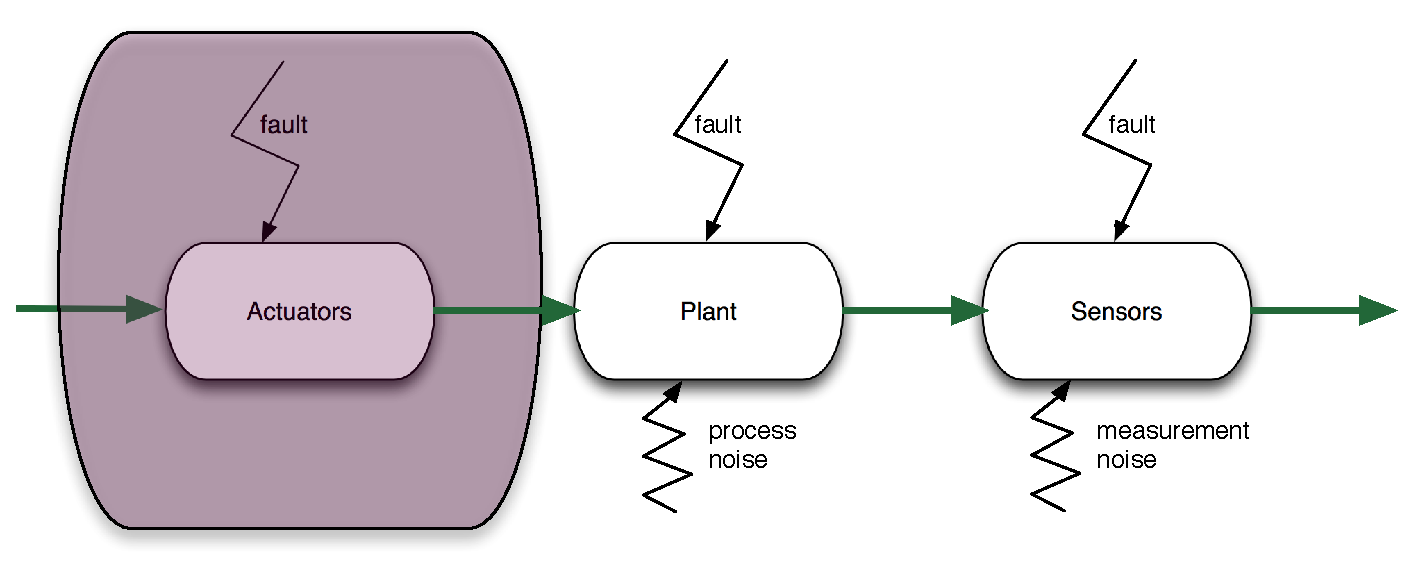
\includegraphics[width=15cm]{figures/faultsInTheSystem}    % The printed column width is 8.4 cm.
\caption{Faults altering the system } 
\label{fig:faultsInTheSystem}
\end{center}
\end{figure}


\section{Fault Tolerant Control Systems}

\subsection{Terminology}\label{ch2:terminology}

Since fault tolerant control is comprised of a set of different disciplines and a relatively 
new topic, the terminology is not solid. FDI could be a proper example to this ambiguity. 
In some works, it stands for Fault Detection and Isolation while in some other 
Fault Detection and Identification, which could also named after Fault Detection and Diagnosis, 
meaning that identification is added to Fault Detection and Isolation \cite{zhang2008bibliographical}.

One of the first attempts to unify the terminology is carried out by IFAC SAFEPROCESS 
technical committee in 1996 and published by \cite{isermann1997trends}. Fault, failure, 
and the methodology to handle those such as fault detection, fault isolation, fault identification, 
fault diagnosis and supervision terms explained separately to avoid the ongoing ambiguity 
in this field. Although fault detection methods are clearer in the work, difference between 
the methods for two steps of fault diagnosis, namely the fault isolation and fault 
identification is not very obvious

\subsection{Conventions for a Safe Flight}\label{ch2:conventions}

The widely used method to increase reliability is to use more reliable components 
and/or hardware redundancy. Both requires an increase in the cost of the UAS 
conflicting one of the main reasons of UAS design itself band consumer expectations 
\cite{angelov2012sense}. To offer solutions for all different foreseen categories of 
airspace, a variety of approaches should be considered. While hardware redundancy 
could cope with the failure situations of UAVs in the certified airspace, it may not be 
suitable for UAVs in open or some subsets of specific categories due to budget 
constraints. Analytical redundancy is another solution, may be not as effective and 
simple as hardware redundancy, but relies on the design of intelligent methods to 
utilize every bit of information onboard aircraft wisely to deal with the instances.  

There are three approaches to achieve safe FTC in standard flight conventions. 
First one is the fail operational systems which are made insensitive to any single 
point component failure. The second approach is the fail safe systems where a 
controlled shut down to a safe state is practiced whenever a critical fault is pointed 
out by a sensor. The level of degradation assures to switch to robust (alternate) or 
direct (minimal level of stability augmentation independent of the nature of the fault) mode. 
Switching from nominal mode to the robust and direct modes leads to a decrease 
in the available GNC functions. This causes a degradation in ease of piloting. And 
also some optimality conditions could have been compromised. The third approach 
is fault tolerant control systems in which redundancy in the plant and the automation 
system is employed to design software that monitors the components and takes in 
action whenever needed. The strategy is most probably to try to keep plant availability 
and accept reduced performance \cite{blanke2000fault}.

RECONFIGURE project of FP7 \cite{goupil2015overview} aims to attack at this 
problem of piloting degradation and optimality compromisation by attacking 
Flight Parameter Estimation (FPE) which is the online estimation of aircraft parameters, 
FDD and FTC in case of off-nominal events \cite{RECONFIGURE} They utilize a black 
box nonlinear model of aircraft and The project uses some outputs of a previous FP 7 
project ADDSAFE leaded by Deimos Space \cite{ADDSAFE}.

\subsection{Methods for Fault Tolerant Control Systems}\label{ch1:methodsFTCS}

Among different categorizations for the fault tolerance, there are options to handle 
faults on-line or off-line. Employing fault diagnosis schemes on-line is a way to 
achieve fault tolerance. In this case, as soon as a fault detected, a supervisory 
agent is informed via a discrete event signal. Then accommodation of the faults 
are handled either with the selection of a predetermined controller for the specific 
fault case, or by designing the action online with real-time analysis and optimization \cite{blanke2000fault}.

Another common categorization of FTCS is passive and active FTCS. In passive FTCS, 
the flight controller is designed in such a way to accommodate not only the 
disturbances but also the faults. Active FTCS first distinguishes the fault via fault detection 
and diagnosis module and then switch between the designed controllers specific to the 
fault case or design a new one online \cite{angelov2012sense}. While active FTCS 
requires more tools to handle faults as seen in Fig.~\ref{fig:FTCS}, for faults 
not predicted and not counted for during the design of the robust controller, this method 
most probably fails. 

\begin{figure}
\begin{center}
%\includegraphics[width=11.3cm]{figures/FTCmethods}    % The printed column width is 8.4 cm.
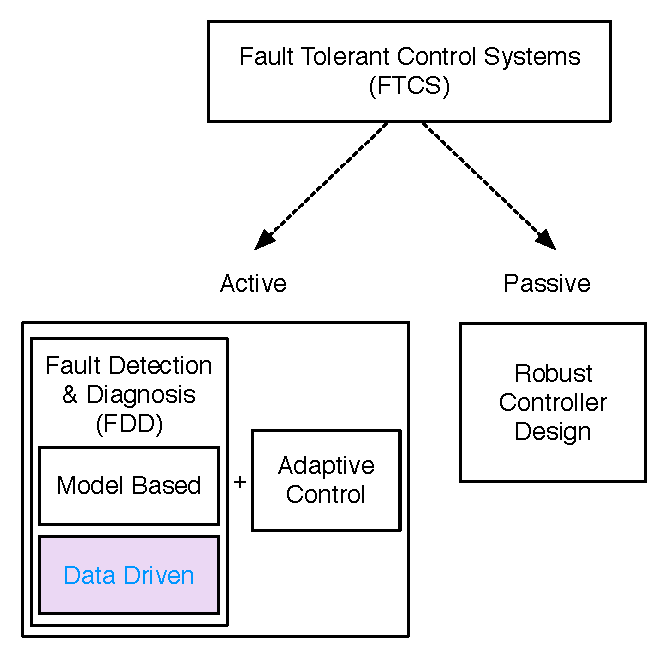
\includegraphics[width=11.3cm]{figures/FTCS}
\caption{Variations of fault tolerant control systems } 
\label{fig:FTCS}
\end{center}
\end{figure}


Even with a long list of available methods, aerospace industry has not implemented 
FTC widely, except some space systems, due to the evolving nature of the methods, 
the tricks coming with the nonlinear nature of the problem, design complexity and high 
possibility of wrong alarms in case of large disturbances and/or modeling uncertainties. 
So the already carried reliability measures concerning the hardware redundancy is 
now the preferred way because of its ease and maturity being implemented on various 
critical missions with considering human lives.

\subsection{Fault Detection and Diagnosis}

FDD is handled in two main steps; fault detection and fault diagnosis. Fault diagnosis 
encapsulates fault isolation and fault identification. The methods for detection and 
diagnosis are investigated for their frequency of utilization separately for sensor, 
actuator, process and controller faults in \cite{isermann1997trends}. FDD should 
not only be sensitive to the faults but also robust to the model uncertainties and 
external disturbances.

Two distinct options to proceed in analytical redundancy are the model based 
approaches and data-driven approaches. They form the two ends of a continuous 
solution set line, so utilizing them in a combination might end up with better solutions. 
Model based fault diagnosis highlights the components of a system and the connections 
in-between, and their corresponding fault modes. Data driven fault diagnosis rely on 
the observational data and prefers dense, redundant and with a  frequency larger than 
the failure rate. 

% This is an example of how you would use tgrind to include an example
% of source code; it is commented out in this template since the code
% example file does not exist.  To use it, you need to remove the '%' on the
% beginning of the line, and insert your own information in the call.
%
%\tagrind[htbp]{code/pmn.s.tex}{Post Multiply Normalization}{opt:pmn}

\subsubsection{Model Based Methods}

In model based approaches, relations between measurements and estimated 
states are exploited to detect possible dysfunction. The most common ways to 
implement a model based approach is to estimate the states, estimate the model 
parameters, or parity-space. The accuracy of the results depend on the type of 
faults (additive or multiplicative). Additive faults affects the variables of the process 
by a summation whereas the multiplicative faults by a multiplication.  When only 
output signal can be measured, signal model based methods can be employed for 
fault detection such as Bandpass filters, Spectral analysis(FFT) and maximum entropy estimation. 
For the case, both the input and output signals are available, the utilized methods 
for fault detection are called the process based methods: State and output 
observers(estimators), Parity equations and Identification and parameter estimation. 
They generate residuals for state variables or output variables. When previous works 
investigated, it is concluded that the most widely used technique for sensor and actuator 
faults is the state and output observers (estimators) and for process faults, identification 
and parameter estimation \cite{isermann1997trends}.

The output of the model based fault detection methods is the stochastic behaviour 
with mean values and variances. With the use of change detection methods, deviations 
from the normal behavior can be detected. For that purpose, three available methods 
considered are, mean and variance estimation, likelihood-ratio-test and Bayes decision, 
run-sum test andtwo-probe t-test. Fault detection is only supported by simple threshold 
logic or hypothesis testing in most of the applications \cite{isermann1997trends}.

A bunch of studies discovers the band of different approaches for model-based fault detection. 
Detecting sensor and actuator faults via state estimation, utilizing an EKF is applied to a 
F-16 model in \cite{hajiyev2005sensor}. Parameter identification via $H_{\infty}$ filter 
is used to indicate icing in \cite{melody2001h}.

A drawback of model-based approaches is that they require accurate model of the 
aircraft for successful detection. In a small UAV system susceptible to various 
uncertainties/disturbances and most of the cases does not have an accurate model, 
leading a model-based approach might fail. And also, a mathematical model of a UAV 
is constructed within the flight envelope, and does not necessarily describe the 
possible dynamics invoked by a failure on-board.

A way to handle that is to offer solutions to cope with the uncertainties. 
A fairly old study in 1984, investigates the design problem FDI systems robust to 
uncertainties within the models. One of the two steps of FDI, two steps being the 
residual generation and decision-making, is targeted. They offer to handle model 
uncertainties, by designing a robust residual generation process \cite{chow1984analytical}. 
Another study deals with model uncertainties by determining the threshold of the residual 
in a novel way with an application to detect aileron actuator fault \cite{rotstein2006fault}. 
\cite{sharma2007fault} utilize two cascade sliding mode observers state estimation and 
fault detection to guarantee staying in sliding manifold in the presence of unknown 
disturbances and faults. 
% This is an example of how you would use tgrind to include an example
% of source code; it is commented out in this template since the code
% example file does not exist.  To use it, you need to remove the '%' on the
% beginning of the line, and insert your own information in the call.
%
%\tgrind[htbp]{code/be.s.tex}{Block Exponent}{opt:be}

\subsubsection{Data-Driven Methods}

Model-based approaches had various successful applications until now, 
most of them assuming accurate model is available on-board. With the new 
era of UAVs, the airspace is expected to be populated by an abrupt increase 
in the number of UAVs. The variety of UAVs, expense of accurate modeling 
practices, the difficulty in modeling the behavior of UAV in case of failures, 
call for alternative approaches for the quite challenging problem of FDD. 
The increased efficiency of sensors on-board, the increase in the computational 
capabilities of autopilot processors, and the advances in machine learning 
techniques in the last decade may offer efficient data-driven solutions to FDD.

In data driven methods, a detailed knowledge about the internal dynamics 
of the system is not necessary. The data available is the source of information 
with regard to the behavior of the system. Supervised learning, which requires 
to label the fault cases previously in the training data, is usually utilized for 
data-centric inference of causes. In case of an unlabeled fault, the result is 
expected as a probability distribution of the available normal modes, identified 
fault labels and a probable unknown fault. What is needed at that point is to 
first detect and localize the fault and then to consult domain experts for labeling 
for further integration of this fault into the diagnosis scheme \cite{dataCentricDiagOffline}.

\cite{gui2002fault} argues artificial intelligent methods for fault detection of complex 
systems. Comparison between PCA and model based stochastic parity space 
approaches is given in \cite{hagenblad2004comparison}.
In \cite{li2016data}, the authors argues to use dynamic PCA since UAV flight 
controls is a dynamic system itself and DPCA can reflect unknown disturbances, 
while model-based approaches can only model typical disturbance.  


\section{Safe Integration of Drones into Airpace}
Air safety authorities are forced to develop regulations for UAS due to incidents 
disturbing public safety and demands from companies who desire to utilize them. 
There has been numerous studies, from both the FAA in US and EASA in Europe, 
but none of them decided on a regulations set for the UAVs to satisfy. Improvement 
of the reliability of the flight is considered to be one of the main obstacles for 
integrating UAVs into civil airspace. To achieve a safe flight is not an easy task 
considering the unknowns of the systems, environment and possible system faults 
and failures to emerge. To tackle the safety challenges and help the regulation 
development, NASA is currently carrying out a four years research program (up to 2019) 
to enable Unmanned aircraft traffic management solutions which are structured yet 
flexible when needed. To ensure safety, this integration needs to be achieved through 
airspace management and UAS reliability.

The preliminary airspace designs, like the one proposed by Amazon, identify different 
zones depending on the UAS capabilities, population density and altitude. Plus, 
different national rules and their progressive refinement pushes to cope with a variety 
of requirements. Open source and modular architectures are key to adapt these 
requirements. As a specific example, NASA's UTM builds, later to be refined by FAA, 
make modularity essential for UAS software to follow their evolution. 

Concerning reliability, current regulations focus on flight constraints but they might be 
expected to involve regulations on software and hardware components as well. 
In such case, the increased cost will be inevitable for the demands of certification. 
This could put too many constraints on UAS manufacturers who desire to access the G airspace. 

In Europe, Regulation (EC) No 216/2008 mandates the European Aviation Safety Agency 
to regulate Unmanned Aircraft Systems (UAS) and in particular Remotely Piloted Aircraft 
Systems (RPAS), when used for civil applications and with an operating mass of 150 Kg or more.

\section{UAVs populating airspace}\label{ch2:certificationOfAnalyticalApproaches}

The cost effectiveness and reachability of commercial off-the-shelf elements, and 
shrinking size of electronics serve as a perfect environment for small flying vehicles 
to emerge. Although inherited as military purposes in its infancy, nowadays \gls{uas} 
are becoming efficient platforms for scientific/commercial domains. They offer 
benefits in terms of cost, flexibility, endurance as well as realizing missions that 
would be impossible with a human onboard. 
Increasing usage of these vehicles for a variety of missions, such as defense, 
civilian tasks including transportation, communication, agriculture, disaster mitigation 
applications pushes demand on the airspace. Furthermore, this congestion is predicted 
to accelerate with the growing diversity of these systems. 

Commercial advantages, offered by these efficient systems, are already targeted by 
big companies worldwide, specifically in the US. The airspace regulatory authorities 
seem to be squeezed in between the companies, demanding a fast as possible 
access to airspace, and the concerns of the public about potential privacy breaches, 
safety and liability issues \cite{droneDisasters,droneImageProblem}. Even with today's 
strictly regulated airspace, reported occurrences show that there are hurdles to solve 
before a further integration of \gls{uas} to airspace.

Advent of the new era of \gls{uas} seems to be hold by an unseen barrier of lack of 
regulatory framework for now. Different institutions all over the world, specifically \gls{nasa} 
and faa in US, easa in Europe and international bases such as \gls{icao} are addressing 
safe integration of \gls{uas} in airspace. Although the approaches of regulatory bodies 
may vary, the aim remains the same: safe integration as soon as possible. 

The tackles of safety during integration of \gls{uas} to airspace refer to different technical 
and organizational aspects including but not limited to control of traffic in segregated and 
non-segregated airspace, reliable communication, robust control of the \gls{uav}, trajectory planning, detect\&avoid.


\section{Modularity}\label{ch2:modularity}

The current evolving nature of regulations and the variety of organizations in charge 
of the airspace rule making calls for flexible solutions to cope with these fruitful environments. 

\subsection{Airspace Categorization}
The \gls{uas} in the \gls{nas} project points to a performance-based routine access to 
all segments of the national airspace for all unmanned aircraft system classes, after the 
safety and technical issues are addressed thoroughly. As a start, \gls{nasa} and faa 
seem to have a short term goal to integrate \gls{uas} in low-altitude airspace as early 
as possible. They further aim to accommodate increased demand safely, efficiently in 
the long term. \gls{nasa} and faa seem to handle the airspace above 500 feet and the 
one below separately. easa, tasked by the European Union, is planning a risk based approach, 
accommodating the \gls{uas} in the airspace under three different categories, low risk, 
specific and high risk. Both regulators seem to categorize the airspace and scale regulatory 
needs according to some criteria. To answer different needs of different categories, flexibility 
given by the high level of modularity of open source autopilot systems will be a handy tool. 

\subsection{National Regulations}
Circulation of \gls{uas} internationally is somewhat prevented by the Chicago convention 
unless an agreement holds between Contracting States \cite{A_NPA_EASA2015}. \gls{icao} is aiming 
to develop international standards and recommended practices to which the member states 
could refer to when developing their national civil aviation regulations. Even though a similar 
base is aimed, national aviation legislations will not be the same because of the different 
expectations of nations about \gls{uas} aviation. 

\subsection{Accommodating evolution of regulations}
Prescriptive rules seem to cause some difficulties since the technical area on \gls{uas} 
systems develop rapidly \cite{A_NPA_EASA2015}. Innovations both on the aircraft and the operation 
type of \gls{uas} will accelerate especially after the regulations are set. Thus, regulatory 
bodies call for refinable operational requirements and system architectures to evolve into 
a safer and efficient integration of \gls{uas} into airspace. The systems to cope with the 
regulations should also be modular and flexible in order not to be superseded by the 
innovations in the area. 
Thus, the aviation regulatory bodies aim to achieve designs with flexibility where possible, 
structure where needed. Having flexible hardware and software points to modularity, which 
is pretty much best supported via open source systems.



\section{Congestion management}\label{ch2:congestion}

According to \textit{UAV Factory}, one of the large European \gls{uas} companies, 
``The future of the UAV industry is likely to be shaped by airspace congestion'' 
\cite{europe_report_civilian_drone}. Indeed, high level airspaces are getting crowded 
and large scale solutions, such as NextGen (US) or SESAR-JU (EU), are necessary to 
increase airspace capacity while maintaining the current safety levels. However, there is 
no such management solution existing for \gls{vll}. Yet, large projects like Amazon's 
Prime Air and Google's Project Wing are already waiting to populate the \gls{vll} airspace.	
	
Part of the congestion management problem is to avoid conflicts, and more importantly 
collisions, between \gls{uas} through strategic deconfliction and safety nets.
Another mission of the congestion management system is to make sure that \gls{uas} 
do not go where they are not supposed to go, thus requiring geofencing. In order to implement 
the previously mentioned systems, the \gls{uas} autopilot needs to be able to perform complex 
operations, e.g. static waypoints following is likely to be insufficient.

In the following, we divide these issues into four topics of interest: 4-D trajectory management, 
geofencing, safety nets, complex operations.
	
\subsection{4-D Trajectory Management}
As noted in \cite{erzberger_4D_2002}, 4-D trajectories will be central in future airspace 
management methods. The principle of 4-D trajectory management is to have every 
\gls{uas} broadcast its trajectory up to some time horizon and receive \gls{utm}'s 
clearances under the form of trajectories. The trajectory information contains a path, 
the series of points through which the \gls{uas} will pass, and times associated to each of these points. 
Thanks to this information, the idea is to perform pro-active deconfliction, as 
explained by Thomas et al. in \cite{thomas_4D_2015}. In clear, it implies that \gls{utm} 
detects future conflicts along the trajectories of all \gls{uas} and deconflicting them 
as safely and early as possible. 
				
\subsection{Safety Nets}
Trajectory deconfliction is the first step to manage congestion, however safety nets 
are also part of the congestion management. Indeed, safety nets such as self-separation 
and collision avoidance allow \gls{uas} to fly close to each other while preserving an 
acceptable safety level.
		
\subsection{Geofencing}
Keeping \gls{uas} away from each other is an important point. But keeping them 
out of forbidden areas is also crucial. Geofencing allows determining no-fly zones 
where the \gls{uas} should not enter.

To accommodate land owners while managing traffic and limiting congestion, Foina et al. 
\cite{foina_air_parcelle_2015} proposed a participative dynamical airspace management 
method: the air-parcel model. It allows land owners to authorize/forbid flights over their 
lands through a web interface. However, this type of approach asks from the \gls{uas}s 
to be able to handle dynamical geofencing. Plus, though initially this model considers only 
cuboid parcels, the need for more precise airspace shapes may emerge making 3-D geofencing a need.
	
\subsection{Complex Operations}
Having 4-D trajectory management, safety nets and geofencing is useless if the \gls{uas}s 
cannot follow the instruction from \gls{utm} regarding these tools. Indeed, new \gls{utm} 
paradigms imply being able to change flight plans dynamically to answer to \gls{utm} demands. 
In \cite{wargo_complex_2015} two types of complex operations examples are mentioned: 
space transition corridors and temporary flight restriction. Both these airspace management 
methods require from the \gls{uas} to be able to modify its flight plan according to new \gls{utm} instructions.
		

\section{Reliability}\label{ch2:reliability}

Improvement of the reliability of the flight is considered to be one of the main goals for 
integrating military \gls{uav}s into civil airspace according to Unmanned systems roadmap 
by US Office of the Secretary of Defense, DoD \cite{UnmannedSystemsRoadmapDoD}. 
Compared to manned counterparts, \gls{uav}s experienced failures with a frequency of two 
orders of magnitude more in the military domain.  Although this changed last years with 
the technological improvements, making the \gls{uav}s as reliable as early manned military 
aircraft, it seems not enough from the DoD perspective. This can be realized by checking 
the biggest chunk of control technologies budget for research and development, which is 
health management and adaptive control.

To achieve a safe flight is not an easy task considering the unknowns of the systems hardware, 
environment and possible system faults and failures to emerge. Also, increasing demand on 
cost effective systems, resulting in smaller sensors and actuators with less accuracy, 
impose the software to achieve even more. The expectation that \gls{uav}s should be less 
expensive than their manned counterparts might have a hit on reliability of the systems. 
Cost saving measures other than the need to support a pilot/crew onboard or decrement 
in size would probably lead to decrease in system reliability. 

\subsection{\gls{sme}s and Certification Costs}

Utilizing drones for quicker and cheaper deliveries could be rewarding for \gls{sme}s 
since cost per mile of a drone is less then 1 / 30 of the average diesel truck. Being an 
early bird might put the \gls{sme}s in an advantageous position, considering the increase 
in the capabilities of the drones with inevitable acceleration thrusted by research activities 
and their widened application areas. 

Nevertheless, the fairly cheap access to drones and their relatively cheap utilization cost 
does not seem to be enough to put them to air right now due to the heavy cost of certification 
and regulatory hurdles \cite{UAVreliabilityStudy}. In this concern, capable open source solutions 
could be a good way to loosen the tie.  Otherwise, \gls{sme}s, an important factor in drone 
business might not survive. Even worse, they might operate them without relevant permission, 
scarifying a substantial fine as reported by Civil Aviation Authority (CAA). This will compromise 
security in the system contradicting the hopes for reliable integration of drones into airspace. 

\subsection{Individuals and Education}

Individuals, as well as \gls{sme}s, suffer from the same budget constraints. Personal \gls{uav} 
usage counts for a substantial amount of the drone ecosystem.  Both US and European 
authorities mention the importance of individuals in utilizations of drones. There is a community 
with a passion of aviation and potential, but most probably not very experienced.  

\subsection{Flight Heritage for Risk Assessment}

Drone industry being extremely innovative, technical developments could supersede the 
prescriptive rules as regulations. Thus a solution might be to follow a risk based approach 
rather that to have strict rules to cope with. Predicted regulations in Europe seems to evolve 
under different categories dedicated to specific operation risks. Flight heritage and occurrence 
reporting is expected to be an inevitable part of safety risk assessment to achieve reliable flight. 

\subsection{Support for real time planning and onboard vehicle automation}
To access low-altitude airspace with the use of small unmanned aircraft safely, an important 
ability could be to implement real-time planning and on-board vehicle automation. Amazon 
offers that this approach will allow some flexibility to adapt to variable situations such as 
weather changes, severe winds or any other emergency needs.

To conclude, the introduction of \gls{uas}s in the \gls{vll} airspace comes with numerous challenges. 
Though various ways to address them have been proposed, there is still no certainty about how it will be done in the end.

One sure thing is that it will involve two main actors: \gls{utm} and \gls{uas}s. This work focused on the later.	

\section{Certification of analytical approaches NOT FINISHED }\label{ch2:certificationOfAnalyticalApproaches}


Due to the lack of the modeling for interaction in-between different FPE  (Flight Parameter Estimation), FDD and FTC modules in simulations, leaves them free from practical limitations, offering a long way to go for these analytical methods to be certified. 

[REF : certificationOfFDD]
[REF : clearanceOptimBased]


safety issues

http://www.techrepublic.com/article/12-drone-disasters-that-show-why-the-faa-hates-drones/

%FP7_RECONFIGURE REF : FP7RECONFIGUREgeneral page : 978 starting with 4 980 section 4. VERIFICATION AND VALIDATION

Regulations EU : https://easa.europa.eu/unmanned-aircraft-systems-uas-and-remotely-piloted-aircraft-systems-rpas

The increased cost will be inevitable for the demands of certification. REF : UAVreliabilityStudy

This increment could be even beyond expectations that it could lead to a cancellation of project:  REF : http://www.defenseindustrydaily.com/euro-hawk-program-cleared-for-takeoff-03051/

Regulations US : 

US Delivery Drones (News from Guardian http://www.theguardian.com/technology/2015/nov/06/alphabet-and-facebook-compete-with-secret-drone-plans)
--------------------
Even if the companies solve the technical challenges of keeping drones aloft for long periods, sharing data via lasers and serving city-sized areas, both Alphabet and Facebook still face regulatory hurdles. Neither company has been granted a waiver to the current FAA blanket ban on the commercial operation of unmanned aircraft.

Alphabet has applied for an exemption, called ?333? after a section of the FAA regulations, for its Project Wing delivery drones, but that is yet to be granted and in any case would only clear operation to a maximum height of 400ft. Google has also been testing its delivery drones in the US under a Certificate of Waiver or Authorization (COA) with Nasa, which permitted flights intended to help Nasa develop an automated air traffic control system for low-flying drones. This would not apply to drones flying far above other manned and unmanned aircraft.

?There?s not a lot to run into between 60,000 and 90,000 feet,? says Cummings. ?But I?m sure regulators would be deeply suspicious if Google and Facebook were flying these over the US.?

Facebook and Alphabet would not comment.

What's really standing in the way of drone delivery?
---------------------------------------------------------
http://www.theverge.com/2016/1/16/10777144/delivery-drones-regulations-safety-faa-autonomous-flight


 SORASORA SORA SORA Fig.~\ref{fig:sora_barriersSmallerVersion}
\begin{figure}
\begin{center}
\includegraphics[width=24cm,angle=90,origin=c]{figures/sora_barriersSmallerVersion}    % The printed column width is 8.4 cm.
\caption{SORA structure: threats, threat barriers, hazard, harm barriers, harms} 
\label{fig:sora_barriersSmallerVersion}
\end{center}
\end{figure}


%% This is an example first chapter.  You should put chapter/appendix that you
%% write into a separate file, and add a line \include{yourfilename} to
%% main.tex, where `yourfilename.tex' is the name of the chapter/appendix file.
%% You can process specific files by typing their names in at the 
%% \files=
%% prompt when you run the file main.tex through LaTeX.
\chapter{Nonlinear Aircraft Model}

The movement of any object can be represented by changes in its location (translation) or changes in its attitude (rotation) or a combination of both. 
Motion of an aircraft usually involves both translation and rotation. 
Studying aircraft motion is complicated since those two motions are coupled, e.g a rotation might cause a change in aerodynamic forces which affects the translation. 
Thus, to ease the process, the motion is broken into easier problems utilizing some assumptions. 
Such an assumption for the aircraft motion is to assume that the aircraft is a point mass, all its mass is collected at its center of gravity, so translates from one point to the other. 
Then, the aircraft's rotation is investigated by no longer assuming it as a point mass but a rigid body in space.
In this chapter, modeling both of these motions is presented in detail.
  
\section{Attitude motion modeling}

Rotation is a change in an object's attitude. 
A change in attitude is modeled using rotations about the center of gravity.  
This section derives the equations for rotation (attitude motion) in detail. 
For the reader who would like to skip the derivation of these equations, equations for attitude kinematics and attitude dynamics can be found in Equ.~\ref{eqn:compactKinematics} and Equ.~\ref{eqn:attitudeDynamics} respectively.

Rotations are directly affected by external torques and moments while translations are directly affected external forces. 
Also, attitude of an aircraft during translation affects the aerodynamic forces causing changes in translation.

A force applied at a distance from the center of mass causes a rotation.
A very common approach in aircraft control is to balance those rotations, by trimming the aircraft, such that the aircraft will not rotate.

In this section, attitude motion is represented with kinematic and dynamics equations. 
First different parametrization of attitude, such as Euler angles and quaternions, are discussed. 
Then, kinematic and dynamic equations of attitude motion are derived for a general rigid body. 
These equations are later specified for the aircraft as the rigid body of interest. 

\subsection{Attitude representations}
Let $\bm{b_1}, \bm{b_2}, \bm{b_3}$ be a triplet of unit vectors, representing an orthogonal coordinate system attached to a rigid body such that

\begin{equation}
\label{eqn:unitVectors}
\bm{b_1}\times \bm{b_2}= \bm{b_3}
\end{equation}

The rigid body is composed of points, which do not experience any distance change in between during motion of the body. 
The problem of representing attitude can simply be thought of specifying the orientation of this triplet with respect to some reference frame A such as in Fig.~\ref{fig:theTwoFrames}.

\begin{figure}
\begin{center}
%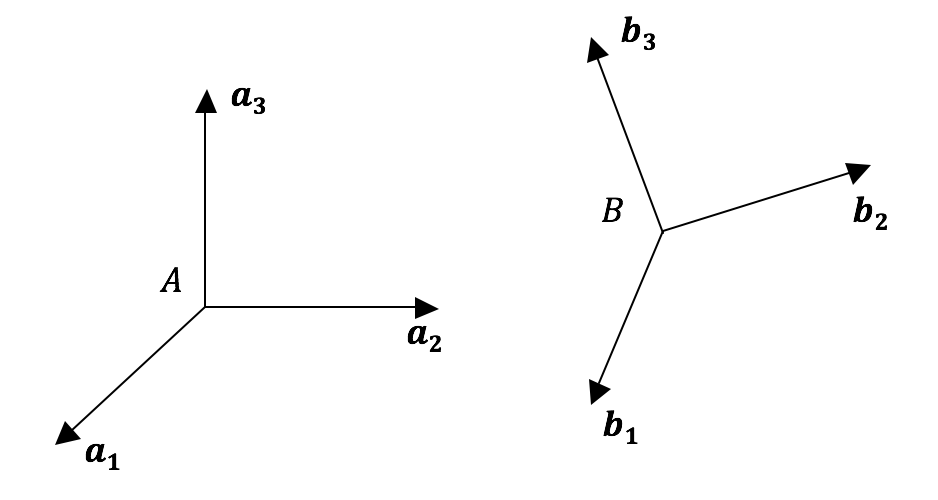
\includegraphics[width=8.3cm]{figures/theTwoFrames}    % The printed column width is 8.4 cm.
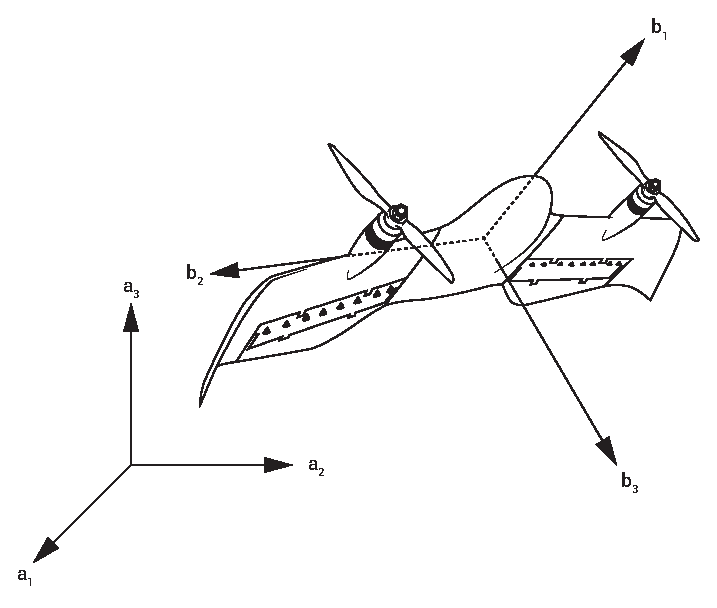
\includegraphics[width=13cm]{figures/DarkoAxesElgiz}    % The printed column width is 8.4 cm.
\caption{Attitude representation is simply specifying the orientation of 
aircraft body axes $\bm{b_1}, \bm{b_2}, \bm{b_3}$ in the reference frame A} 
\label{fig:theTwoFrames}
\end{center}
\end{figure}

Expressing the basis vectors $b_1, b_2, b_3$ of B in terms of basis vectors $a_1, a_2, a_3$ of A is given by :

\begin{align}
\label{eqn:C_B_A}
\begin{split}
\bm{b_1} = C_{11}\bm{a_1} + C_{12}\bm{a_2} + C_{13}\bm{a_3}  ,
\\
\bm{b_2} = C_{21}\bm{a_1} + C_{22}\bm{a_2} + C_{23}\bm{a_3}  ,
\\
\bm{b_3} = C_{33}\bm{a_1} + C_{32}\bm{a_2} + C_{33}\bm{a_3}  .
\end{split}
\end{align}

where $C_{ij} \equiv {\bm{b_i} \cdot \bm{a_j}} $  is called direction cosine as it corresponds to the cosine of the angle between  $\bm{b_i}$ and $\bm{a_j}$. 
When the previous equation set is written in matrix form, we have :

\begin{equation}{\label{eqn:C_B_Amatrix}}
\begin{bmatrix}
\bm{b_1}\\[0.3em]
\bm{b_2}\\[0.3em]
\bm{b_3}\\[0.3em]
\end{bmatrix}
=\,
\begin{bmatrix}
C_{11} & C_{12} & C_{13}\\[0.3em]
C_{11} & C_{12} & C_{13}\\[0.3em]
C_{11} & C_{12} & C_{13}\\[0.3em]
\end{bmatrix}
\,
\begin{bmatrix}
\bm{a_1}\\[0.3em]
\bm{a_2}\\[0.3em]
\bm{a_3}\\[0.3em]
\end{bmatrix}
=\,
\bm{C}^{B/A}
\,
\begin{bmatrix}
\bm{a_1}\\[0.3em]
\bm{a_2}\\[0.3em]
\bm{a_3}\\[0.3em]
\end{bmatrix}
\end{equation} 

Here $\bm{C}^{B/A}$ is called the \emph{direction cosine matrix}, also known as \emph{rotation matrix} or \emph{coordinate transformation matrix} from A to B\cite{wie2008space}.  
The direction cosines, the elements of the direction cosine matrix, are not all independent  \cite{wertz1978spacecraftAttitude}.

The direction cosine matrix is an orthonormal matrix as the basis vectors of each reference frames are orthogonal, so

\begin{equation}
\label{eqn:orthonormality}
\bm{C}^{-1} = \bm{C}^{\rm T}
\end{equation}

and

\begin{equation}
\label{eqn:orthonormality2}
\bm{C}\bm{C}^{\rm T} = \bm{C}^{\rm T}\bm{C} = \mathds{1}
\end{equation}

Where $\mathds{1}$ is the identity matrix.
When the orientation is preserved, an additional condition occurs

\begin{equation}
\label{eqn:noRotation}
\begin{vmatrix}
C\\[0.01em]
\end{vmatrix}
=\,
\mathds{1}
\end{equation}

Matrices satisfying the last two properties belong to special orthogonal group SO(3). 
The following relations are valid between $\bm{C}^{B/A}$ - the direction cosine matrix of B relative to A, or the direction cosine matrix from A to B - and $\bm{C}^{A/B}$ - the direction cosine matrix of A relative to B, or the direction cosine matrix from B to A -.

\begin{align}
\label{eqn:C_B_A_vs_C_A_B}
\begin{split}
[\bm{C}^{A/B}]^{-1} = [\bm{C}^{A/B}]^{\rm T} = \bm{C}^{B/A} 
\\
[\bm{C}^{B/A}]^{-1} = [\bm{C}^{B/A}]^{\rm T} = \bm{C}^{A/B}
\end{split}
\end{align}

The direction cosine maps the vectors from reference frame to body frame.  
Let us write an arbitrary vector $\bm{H}$ in the reference frame A and in the body frame B:

\begin{align}
\label{eqn:vectorInRefFrame}
\begin{split}
\bm{H} & = H_1 \bm{a_1} + H_2 \bm{a_2} + H_3 \bm{a_3}
\\
& = H_1^{'} \bm{b_1} + H_2^{'} \bm{b_2} + H_3^{'} \bm{b_3}
\end{split}
\end{align}

Using the direction cosine matrix in the following equation, components of the arbitrary vector $\bm{H}$ is transformed from A to B.

\begin{equation}{\label{transformVectorH}}
\begin{bmatrix}
H_1^{'}\\[0.3em]
H_2^{'}\\[0.3em]
H_3^{'}\\[0.3em]
\end{bmatrix}
=\,
\begin{bmatrix}
 \bm{b_1} \cdot \bm{a_1}  &  \bm{b_1} \cdot \bm{a_2}  &  \bm{b_1} \cdot \bm{a_3} \\[0.3em]
 \bm{b_2} \cdot \bm{a_1}  & \bm{b_2} \cdot \bm{a_2}  & \bm{b_2} \cdot \bm{a_3} \\[0.3em]
 \bm{b_3} \cdot \bm{a_1}  & \bm{b_3} \cdot \bm{a_2}  &  \bm{b_3} \cdot \bm{a_3} \\[0.3em]
\end{bmatrix}
\,
\begin{bmatrix}
 H_1\\[0.3em]
 H_2\\[0.3em]
 H_3\\[0.3em]
\end{bmatrix}
=\,
\bm{C}^{B/A}
\,
\begin{bmatrix}
H_1\\[0.3em]
H_2\\[0.3em]
H_3\\[0.3em]
\end{bmatrix}
\end{equation} 

\subsubsection{Euler Angles}

One of the approaches to represent the attitude is to use Euler angles. 
It is a procedure to rotate three times successively about one of the axis of the rotated body fixed reference frame. 
The first rotation is about any of the fixed body axes. 
The second one is about any of the other two axis which have not been used in the first rotation. 
The third one is about one of the axis which have not been used in the second rotation. 
The result is a combination of 12 sets of rotation types. 
A sequence of rotations about three different axes of reference frame A, describing the orientation of the body frame B with respect to reference frame A can be represented as

\begin{align}
\label{eqn:sequence}
\begin{split}
{\bm{C}}_3(\theta_{3}) & :      A^{'} \leftarrow A   ,
\\
{\bm{C}}_2(\theta_{2}) & :      A^{''} \leftarrow A^{'}   ,
\\
{\bm{C}}_1(\theta_{1}) & :      A^{'} \leftarrow A^{''}  .
\end{split}
\end{align}

The direction cosine matrix B relative to A can be given as;

\begin{equation}
\label{eqn:sequentialOrientation}
\bm{C}^{B/A}= \bm{C}_{1}(\theta_{1}) \bm{C}_{2}(\theta_{2}) \bm{C}_{3}(\theta_{3})
\end{equation}

where $\theta_{1}$, $\theta_{2}$, $\theta_{3}$ are the Euler angles. $\bm{C}_{i}(\theta_{i})$  
denotes a rotation of angle $\theta_{i}$, about the $i^{th}$ axis of the body frame. The orientation of B with respect to A is given as

\begin{align}{\label{eqn:C_B_AmatrixEuler}}
\begin{split}
\begin{bmatrix}
\bm{b_1}\\[0.3em]
\bm{b_2}\\[0.3em]
\bm{b_3}\\[0.3em]
\end{bmatrix}
& =\,
\bm{C}^{B/A}
\,
\begin{bmatrix}
\bm{a_1}\\[0.3em]
\bm{a_2}\\[0.3em]
\bm{a_3}\\[0.3em]
\end{bmatrix}
\\
& =\,
\begin{bmatrix}
1 & 0 & 0\\[0.3em]
0 & \cos\theta_1 & \sin\theta_1\\[0.3em]
0 & -\sin\theta_1 & \cos\theta_1\\[0.3em]
\end{bmatrix}
\,
\begin{bmatrix}
\cos\theta_2 & 0 & -\sin\theta_2\\[0.3em]
0 & 1 &0\\[0.3em]
\sin\theta_2 & 0 & \cos\theta_2\\[0.3em]
\end{bmatrix}
\,
\begin{bmatrix}
\cos\theta_3 & \sin\theta_3 & 0\\[0.3em]
-\sin\theta_3 & \cos\theta_3 & 0\\[0.3em]
0 & 0 & 1\\[0.3em]
\end{bmatrix}
\\
& =\,
\begin{bmatrix}
\cos\theta_2 \cos\theta_3 & \cos\theta_2 \sin\theta_3 & -\sin\theta_2\\[0.3em]
\sin\theta_1 \sin\theta_2 \cos\theta_3 - \cos\theta_1 \sin\theta_3 & \sin\theta_1 \sin\theta_2 \cos\theta_3 + \cos\theta_1 \cos\theta_1 \cos\theta_3 & \sin\theta_1 \cos\theta_2\\[0.3em]
\cos\theta_1 \sin\theta_2 \cos\theta_3 + \sin\theta_1 \sin\theta_3 & \cos\theta_1 \sin\theta_2 \sin\theta_3 - \sin\theta_1 \cos\theta_3 & \cos\theta_1 \cos\theta_2\\[0.3em]
\end{bmatrix}
\end{split}
\end{align}

Rotation sequence can be selected in different ways depending on the needs of the problem. 
An example would be selecting rotation sequence for a transitioning vehicle. The assumption that the pitch angle is constraint to $0<\theta<90^\circ$ for a conventional drone to avoid singularity, is not really feasible for a transitioning vehicle which encounters $-90<\theta<90$ pitch during whole flight envelope. So for such a problem, selecting the sequence as yaw-roll-pitch rather than the conventional yaw-pitch-roll sequence is useful. 

So for such a reason, if the set of rotations are selected in a different way, such as 

\begin{align}
\label{eqn:sequence2}
\begin{split}
{\bm{C}}_2(\theta_{2}) & :      A^{'} \leftarrow A   ,
\\
{\bm{C}}_3(\theta_{3}) & :      A^{''} \leftarrow A^{'}   ,
\\
{\bm{C}}_1(\theta_{1}) & :      A^{'} \leftarrow A^{''}  .
\end{split}
\end{align}

then the direction cosine matrix would differ from Eq.~\ref{eqn:C_B_AmatrixEuler}.

For aircrafts, the Euler angles are called pitch, yaw and roll and can be seen in Fig.~\ref{fig:eulerAngSequence}.

%\begin{figure}
%\begin{center}
%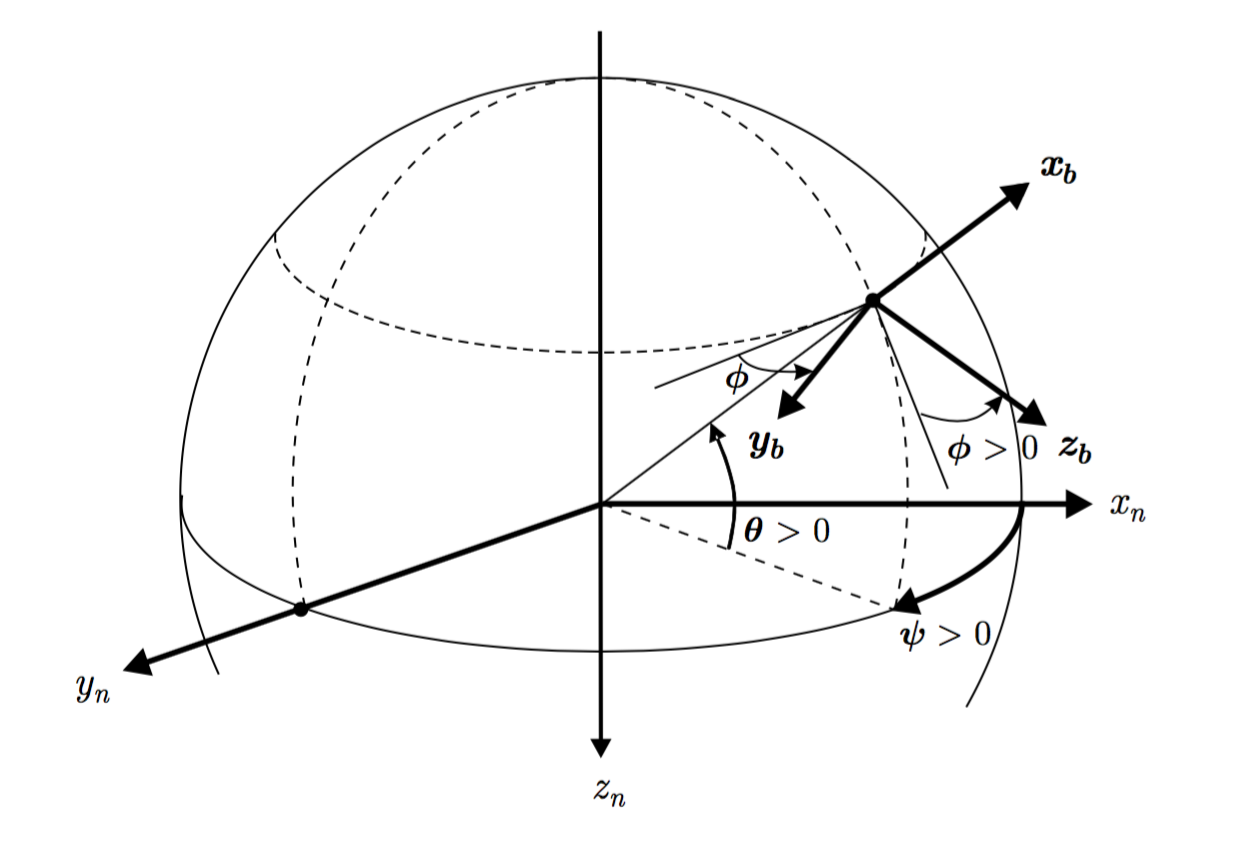
\includegraphics[width=11cm]{figures/eulerAnglesAircraft}    % The printed column width is 8.4 cm.
%\caption{Euler angle sequence \cite{ducard2009fault}} 
%\label{fig:eulerAnglesAircraft}
%\end{center}
%\end{figure}

\subsubsection{Quaternions}

The idea behind this representation is the Euler's \emph{eigen-axis rotation} theorem. 
According to Euler, \say{the most general displacement of a rigid body with one point fixed is a rotation about some axis.} In other words, it states that there exists a unit vector $\bm{e}$, with the property

\begin{equation}
\label{eqn:quat1}
\bm{C}\bm{e}= \bm{e}
\end{equation}

$\bm{e}$ vector has the same components in body and reference frames :

\begin{align}
\label{eqn:quat2}
\begin{split}
\bm{e} & = e_1 \bm{a_1} + e_2 \bm{a_2} + e_3 \bm{a_3}
\\
& = e_1 \bm{b_1} + e_2 \bm{b_2} + e_3 \bm{b_3}
\end{split}
\end{align}
 
Rotating a rigid body about this axis $\bm{e}$, a rotation from any given orientation to any other orientation can be achieved. 
Such an axis is called  \emph{Euler axis}, after the Swiss mathematician and theoretical physicist Leonard Euler (1707-1783).

\begin{landscape}
\begin{figure}
\begin{center}
%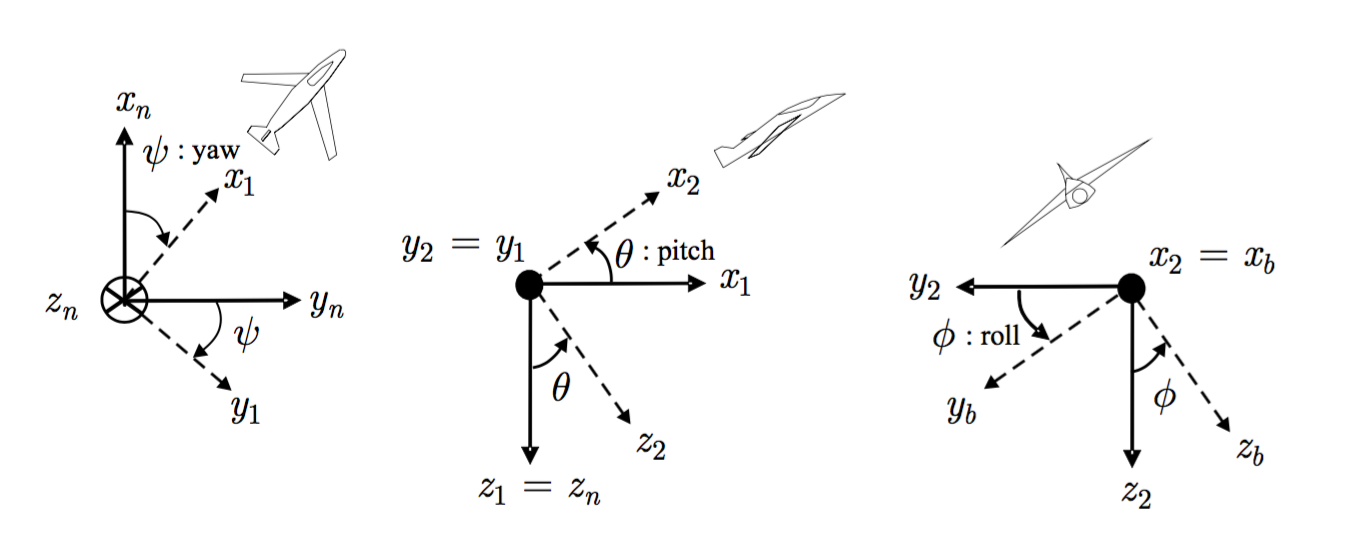
\includegraphics[width=11cm]{figures/eulerAngSequence}    % The printed column width is 8.4 cm.
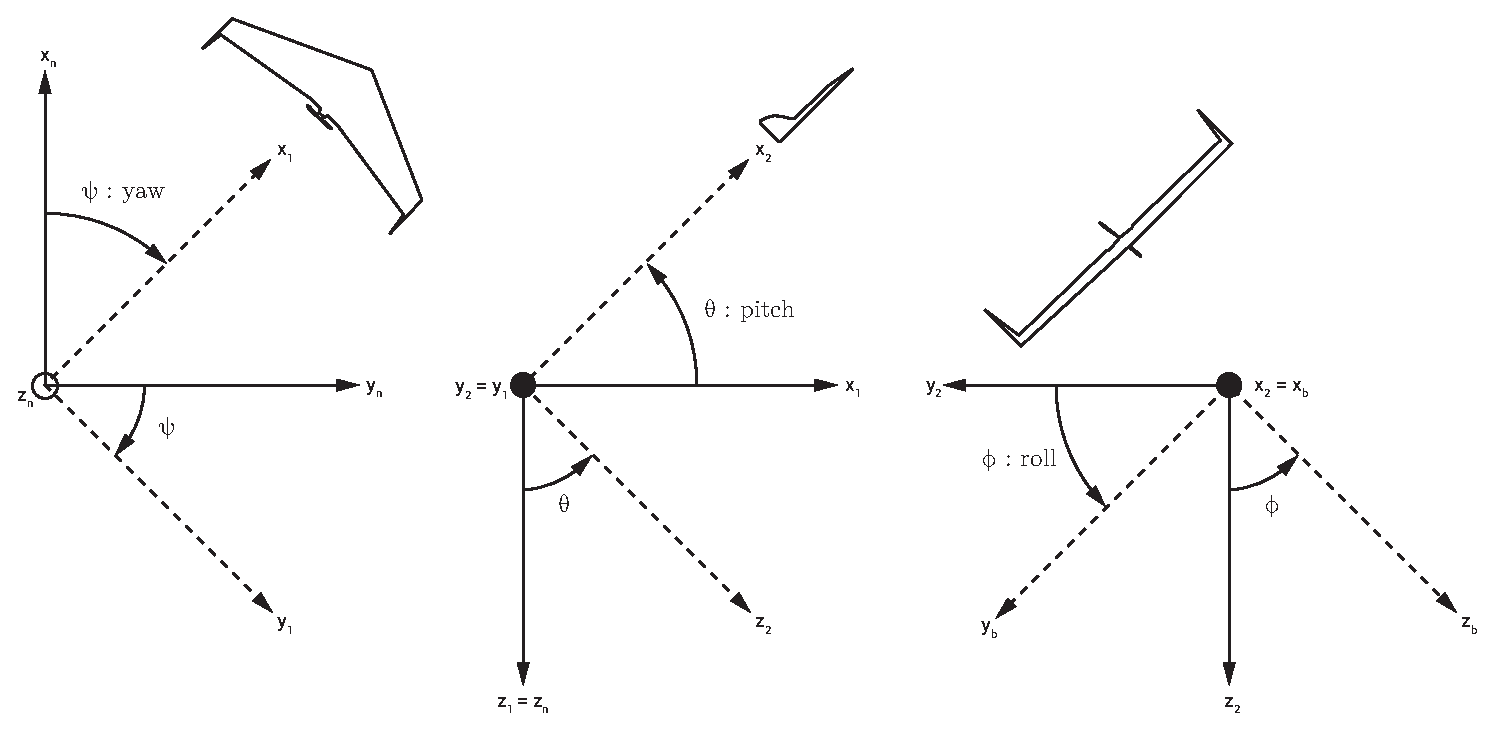
\includegraphics[width=23cm]{figures/ZagiEulerAngleSequence}
\caption{Euler angle sequence \cite{ducard2009fault}} 
\label{fig:eulerAngSequence}
\end{center}
\end{figure}
\end{landscape}

\emph{Euler symmetric parameters}, also known as \emph{quaternions}, are defined as:
 
 \begin{equation}
 \label{eqn:quat3}
\bm{q}
=\,
\begin{bmatrix}
q_0\\[0.3em]
q_1\\[0.3em]
q_2\\[0.3em]
q_3\\[0.3em]
\end{bmatrix}
=\,
\begin{bmatrix}
\cos(\phi/2)\\[0.3em]
e_1 \sin(\phi/2)\\[0.3em]
e_2 \sin(\phi/2)\\[0.3em]
e_3 \sin(\phi/2)\\[0.3em]
\end{bmatrix}
\end{equation}
 
Where $\phi$ is the \emph{Euler rotation angle}. 
Hamilton (1805-1865) is considered to be the first one to mention quaternions. 
For ease of the mathematical representations, we define a vector as :

\begin{equation}
\label{eqn:quat3}
\bm{q} = \bm{e}\sin{(\phi/2)}
\end{equation}

Euler symmetric parameters are not independent, and satisfy the constraint

\begin{equation}
\label{eqn:quatNormConstraint}
\bm{q}^{\rm T} \bm{q} + q_0^2 = q_0^2 + q_1^2 +q_1^2 +q_3^2 = 1
\end{equation}

The direction cosine matrix can also be written in terms of quaternions as below

\begin{align}\label{eqn:Cquat}
\begin{split}
C(\bm{q})
 & =\,
\begin{bmatrix}
q_0^2 + q_1^2 - q_2^2 - q_3^2 & 2(q_1 q_2 + q_3 q_0) & 2(q_1 q_3 - q_2 q_0)\\[0.3em]
2(q_1 q_2 - q_3 q_0) & q_0^2 - q_1^2 + q_2^2 - q_3^2 & 2(q_2 q_3 + q_1 q_0)\\[0.3em]
2(q_1 q_3 + q_2 q_0) & 2(q_2 q_3 - q_1 q_0) & -q_1^2 - q_2^2 + q_3^2 + q_0^2\\[0.3em]
\end{bmatrix}
\\
& = (q_0^2 - \bm{q}^{\rm T}\bm{q} )\mathds{1} + 2\bm{q}\bm{q}^{\rm T} - 2q_0\bm{Q}
\end{split}
\end{align}
 
where

\begin{equation}
\label{eqn:Qmatrix}
\bm{Q}
=\,
\begin{bmatrix}
0 & - q_3 & q_2 \\[0.3em]
q_3 & 0 & - q_1 \\[0.3em]
- q_2 & q_1 & 0\\[0.3em]
\end{bmatrix}
\end{equation}

Given the direction cosine matrix, quaternions can be calculated as

\begin{align}\label{eqn:quat4}
\begin{split}
\bm{q}
& =\,
\begin{bmatrix}
q_1\\[0.3em]
q_2\\[0.3em]
q_3\\[0.3em]
\end{bmatrix}
 =\,
\frac{1}{4q_0}
\begin{bmatrix}
C_{23} - C_{32}\\[0.3em]
C_{31} - C_{13}\\[0.3em]
C_{12} - C_{21}\\[0.3em]
\end{bmatrix}
\\
q_0
& =\,
\pm{\frac{1}{2}}{(1 + C_{11} + C_{22} + C_{33})}^{\frac{1}{2}}
\end{split}
\end{align}

\subsubsection{Attitude parametrization selection}

In 1776, Euler showed that SO(3) has three dimensions \cite{stuelpnagel1964parametrization}. 
Representations with more than three parameters are subject to constraints. 
Also, \cite{stuelpnagel1964parametrization} states that no parameter set 
can be both global and nonsingular. 
So, we are faced with choosing the representation parameters either singular or redundant. 
Euler angle representation has its advantages like having a clear physical interpretation and minimum parameter set achieving no redundancy. 
But due to their important disadvantage, the possibility of having singularities when describing motion, Euler angles are not selected to represent attitude in this study.
Another attitude parametrization, the Gibbs vector, is not very often used, and can be thought that it is an interval step on the way of quaternion parametrization. 
There are other representation types, which are not very often preferred, such as the axis-azimuth representation, which will not be mentioned in this thesis \cite{bak1999spacecraft}. 
Quaternion (Euler symmetric parameters) representation will be used in this study due to their advantageous in simulations, and having no singularities.
Another advantage of quaternions is that, the kinematic equations are linear in terms of quaternions. 
Also, quaternion multiplication offers a useful way of expressing composite rotations. 
With all these preferable properties, quaternions are the choice for attitude representations for many attitude control missions. Table~\ref{arm:attRepSelection} shows a brief comparison of attitude representations \cite{bak1999spacecraft}.\\
In the previous sections, a variety of parameters to represent rotations are identified and inherent properties of each technique have been examined. 
Now it is time to find out how to represent attitude depending on time, namely the equations of motion. 
Equations of motion are generally presented in two sections: the kinematic equations and dynamic equations. 
The kinematic equations provide the relations between the time derivative of the attitude representation and the angular velocity, while the dynamics (or kinetics) equations describe the development of angular velocities under influence of external moments.

\begin{table}
\caption{Attitude parametrizations of the rotation group SO(3) \cite{bak1999spacecraft}}
\label{arm:attRepSelection}
\begin{center}
 \begin{tabular}{||c || c | c ||}
 \hline
 &Number of  &  \\ [0.5ex] 
Representation &parameter set & Properties \\ [0.5ex] 
 \hline\hline
& & Minimal set\\ 
& & Clear physical interpretation\\ 
& & Often computed directly\\ 
 Euler angles   & 3 & Trigonometric functions in rotation matrix \\ 
& & No simple composition rule \\ 
& & Singular for certain rotations \\ 
& & Trigonometric functions in kinematic relation \\ 
 \hline
& & Easy orthogonality of rotation matrix\\ 
& & Bilinear composition rule\\ 
& & Not singular at any rotation\\ 
Quaternions   & 4 & Linear kinematic equations \\ 
& & No clear physical interpretation \\ 
& &One redundant parameter \\ 
& & Simple kinematic relation \\ 
 \hline
& & Minimal set\\ 
Gibbs vector   & 4 & Clear composition rule\\ 
& & Singular for certain rotations \\ 
& & Simple kinematic relation \\[1ex] 
 \hline
\end{tabular}
\end{center}
\end{table}

%\begin{table}
%\caption{Attitude representations comparison}
%\label{tab:attRepSelection}
%\begin{center}
%\begin{tabular}{||l|l||}\hline
%Representation & Number of parameter set & Properties \\\hline
%our	   & friends \\\hline
%\end{tabular}
%\end{center}
%\end{table}


%\begin{table}
%\caption{Armadillos}
%\label{arm:table}
%\begin{center}
%\begin{tabular}{||l|l||}\hline
%Armadillos & are \\\hline
%our	   & friends \\\hline
%\end{tabular}
%\end{center}
%\end{table}


\subsection{Attitude kinematics}

The time evolution of attitude is identified by a set of first order differential equations called the kinematic equations. 
The angular velocity of a reference frame B with respect to a reference frame A, given in the B frame can be written as follows

\begin{equation}\label{eqn:quaternion1}
\bm{\omega}_B^{B/A}
 =\,
\omega_1 \bm{b_1} + \omega_2 \bm{b_2} + \omega_3 \bm{b_3}
\end{equation}

Recalling Eq. ~\ref{eqn:C_B_Amatrix} and orthonomality property in Eq. ~\ref{eqn:orthonormality}

\begin{equation}{\label{eqn:kinematicsDerivation1}}
\begin{bmatrix}
\bm{a_1}\\[0.2em]
\bm{a_2}\\[0.2em]
\bm{a_3}\\[0.2em]
\end{bmatrix}
=\,
\Big[{\bm{C}_B^{B/A}}\Big]^{-1}
\,
\begin{bmatrix}
\bm{b_1}\\[0.2em]
\bm{b_2}\\[0.2em]
\bm{b_3}\\[0.2em]
\end{bmatrix}
=\,
\Big[{\bm{C}_B^{B/A}}\Big]^{\rm T}
\,
\begin{bmatrix}
\bm{b_1}\\[0.2em]
\bm{b_2}\\[0.2em]
\bm{b_3}\\[0.2em]
\end{bmatrix}
\end{equation} 

Taking the time derivative with respect to frame A

\begin{align}{\label{eqn:C_B_Amatrix_timeDerivative}}
\begin{split}
\frac{d}{dt}
\left.
\begin{bmatrix}
\bm{a_1}\\[0.2em]
\bm{a_2}\\[0.2em]
\bm{a_3}\\[0.2em]
\end{bmatrix}
\right|_A &=\,
\Big[{\dot{\bm{C}}_B^{B/A}}\Big]^{\rm T}
\,
\begin{bmatrix}
\bm{b_1}\\[0.2em]
\bm{b_2}\\[0.2em]
\bm{b_3}\\[0.2em]
\end{bmatrix}
+\,
\Big[{\bm{C}_B^{B/A}}\Big]^{\rm T}
\,
\begin{bmatrix}
\dot{\bm{b_1}}\\[0.2em]
\dot{\bm{b_2}}\\[0.2em]
\dot{\bm{b_3}}\\[0.2em]
\end{bmatrix}
=\,
\Big[{\dot{\bm{C}}_B^{B/A}}\Big]^{\rm T}
\,
\begin{bmatrix}
\bm{b_1}\\[0.2em]
\bm{b_2}\\[0.2em]
\bm{b_3}\\[0.2em]
\end{bmatrix}
+\,
\Big[{\bm{C}_B^{B/A}}\Big]^{\rm T}
\,
\begin{bmatrix}
\bm{\omega} \times \bm{b_1}\\[0.2em]
\bm{\omega} \times \bm{b_2}\\[0.2em]
\bm{\omega} \times \bm{b_3}\\[0.2em]
\end{bmatrix}
\\
& =\,
\Big[{\dot{\bm{C}}_B^{B/A}}\Big]^{\rm T}
\,
\begin{bmatrix}
\bm{b_1}\\[0.2em]
\bm{b_2}\\[0.2em]
\bm{b_3}\\[0.2em]
\end{bmatrix}
+\,
\Big[{\bm{C}_B^{B/A}}\Big]^{\rm T}
\,
\begin{bmatrix}
0 & - \omega_3 & \omega_2 \\[0.3em]
\omega_3 & 0 & - \omega_1 \\[0.3em]
- \omega_2 & \omega_1 & 0\\[0.3em]
\end{bmatrix}
\,
\begin{bmatrix}
\bm{b_1}\\[0.2em]
\bm{b_2}\\[0.2em]
\bm{b_3}\\[0.2em]
\end{bmatrix}
\end{split}
\end{align}

If the skew-symmetric matrix can be represented as $\bm{\Omega}$

\begin{equation}\label{eqn:Qmatrix}
\bm{\Omega}
=\,
\begin{bmatrix}
0 & - \omega_3 & \omega_2 \\[0.3em]
\omega_3 & 0 & - \omega_1 \\[0.3em]
- \omega_2 & \omega_1 & 0\\[0.3em]
\end{bmatrix}
\end{equation}

and rearrange the terms

\begin{equation}{\label{eqn:C_dot_T_C_T_Omega}}
\bigg[\Big[{\dot{\bm{C}}_B^{B/A}}\Big]^{\rm T} - \Big[{\bm{C}_B^{B/A}}\Big]^{\rm T} \bm{\Omega} \bigg]
\,
\begin{bmatrix}
\bm{b_1}\\[0.2em]
\bm{b_2}\\[0.2em]
\bm{b_3}\\[0.2em]
\end{bmatrix}
 =\,
\begin{bmatrix}
0\\[0.2em]
0\\[0.2em]
0\\[0.2em]
\end{bmatrix}
\end{equation}

implies

\begin{equation}{\label{eqn:C_dot_T_C_T_Omega2}}
\bigg[\Big[{\dot{\bm{C}}_B^{B/A}}\Big]^{\rm T} - \Big[{\bm{C}_B^{B/A}}\Big]^{\rm T} \bm{\Omega} \bigg]
 =\,
\bm{0}
\end{equation}

Taking the transpose and using the relationship $\Omega^{\rm T} = - \Omega$, the kinematic differential equation for the direction cosine matrix can be written as,

\begin{equation}{\label{eqn:kinematicEquDQM}}
{\dot{\bm{C}}_B^{B/A}} + \bm{\Omega} {\bm{C}_B^{B/A}}
 =\,
\bm{0}
\end{equation}

Angular velocity components, given in the B reference frame can be written as

\begin{align}{\label{eqn:angVelocityKinematics}}
\begin{split}
\omega_1 & = \dot{C}_{21} C_{31} + \dot{C}_{22} C_{32} + \dot{C}_{23} C_{33} \\
\omega_2 & = \dot{C}_{31} C_{11} + \dot{C}_{32} C_{12} + \dot{C}_{33} C_{13} \\
\omega_3 & = \dot{C}_{11} C_{21} + \dot{C}_{12} C_{22} + \dot{C}_{13} C_{23} \\
\end{split}
\end{align}

From that point, derivation depends on the attitude parameters used. 
When the direction cosines and their derivatives are substituted with their equivalents in terms of Euler angles, the result will give the time dependence of Euler angles. 
But in this study, due to the reasons discussed before, quaternions are selected to represent the attitude, so the direction cosines will be written in terms of quaternions,

\begin{align}{\label{eqn:angVelocityQuaternion}}
\begin{split}
\omega_1 & = 2 (\dot{q}_1 q_0 + \dot{q}_2 q_3 - \dot{q}_3 q_2 - \dot{q}_0 q_1) \\
\omega_2 & = 2 (\dot{q}_2 q_0 + \dot{q}_3 q_1 - \dot{q}_1 q_3 - \dot{q}_0 q_2) \\
\omega_3 & = 2 (\dot{q}_3 q_0 + \dot{q}_1 q_2 - \dot{q}_2 q_1 - \dot{q}_2 q_3)\\
\end{split}
\end{align}

Fourth equation comes from the differentiation of the quaternion norm constraint;

\begin{equation}{\label{eqn:kinematicEquDQM}}
0 = 2 (- \dot{q}_0 q_0 + \dot{q}_1 q_1 + \dot{q}_2 q_2 - \dot{q}_3 q_3)
\end{equation}

Writing in matrix form;

\begin{equation}{\label{eqn:kinematicEquAngVel}}
\begin{bmatrix}
0\\[0.2em]
\omega_1\\[0.2em]
\omega_2\\[0.2em]
\omega_3\\[0.2em]
\end{bmatrix}
 =\,
 2\,
\begin{bmatrix}
q_1 & q_2 & q_3 & q_0 \\[0.2em]
q_0 & q_3 & -q_2 & -q_1 \\[0.2em]
-q_3 & q_0 & q_1 & -q_2 \\[0.2em]
q_2 & -q_1 & q_0 & -q_3 \\[0.2em]
\end{bmatrix}
\,
\begin{bmatrix}
\dot{q}_0\\[0.2em]
\dot{q}_1\\[0.2em]
\dot{q}_2\\[0.2em]
\dot{q}_3\\[0.2em]
\end{bmatrix}
\end{equation}
 
As the matrix which is composed of quaternions is an orthonormal matrix, the kinematic equations of motion in terms of quaternions can be given as \cite{wie2008space}

\begin{align} \label{eqn:kinematicArrange}
\begin{split}
\begin{bmatrix}
\dot{q}_0\\[0.2em]
\dot{q}_1\\[0.2em]
\dot{q}_2\\[0.2em]
\dot{q}_3\\[0.2em]
\end{bmatrix}
& =\,
\frac{1}{2}
\,
\begin{bmatrix}
-q_1 & -q_2 & -q_3 & q_0 \\[0.2em]
q_4 & -q_3 & q_2 & q_1 \\[0.2em]
q_3 & q_4 & -q_1 & q_2 \\[0.2em]
-q_2 & -q_1 & q_4 & q_3 \\[0.2em]
\end{bmatrix}
\,
\begin{bmatrix}
0\\[0.2em]
\omega_1\\[0.2em]
\omega_2\\[0.2em]
\omega_3\\[0.2em]
\end{bmatrix} \\
& =\,
\frac{1}{2}
\,
\begin{bmatrix}
-\omega_1 & -\omega_2 & -\omega_3 & 0 \\[0.2em]
0 & \omega_3 & -\omega_2 & \omega_1 \\[0.2em]
-\omega_3 & 0 & \omega_1 & \omega_2 \\[0.2em]
\omega_2 & -\omega_1 & 0 & \omega_3 \\[0.2em]
\end{bmatrix}
\begin{bmatrix}
q_0\\[0.2em]
q_1\\[0.2em]
q_2\\[0.2em]
q_3\\[0.2em]
\end{bmatrix}
\end{split}
\end{align}

And in a more compact form;

\begin{empheq}[box=\fbox]{align}{\label{eqn:compactKinematics}}
\begin{split}
\dot{q}_0 &= -\frac{1}{2} \bm{q}_\nu^T \bm{\omega}_B^{B/A}\\
\dot{\bm{q}}_\nu &= \frac{1}{2}\Big(\bm{q}_\nu^\times + q_0 \bm{I}_3 \Big) \bm{\omega}_B^{B/A} \\
\end{split}
\end{empheq}

where

\begin{equation}\label{skew_symmetric}
\bm{x} ^ \times= \begin{bmatrix} 
0 & -x_3 & x_2 \\
x_3 & 0 & -x_1 \\
-x_2 & x_1 & 0 \\
 \end{bmatrix}
\end{equation}

The sequence of the transformation between frames, effects the final transformation matrix so does the attitude kinematic equations. In the course of this study, the sequence is assumed to be yaw - pitch - roll and the corresponding kinematic equations are given as in Equ.~\ref{eqn:kinematicArrangeYPR}.

And finally the kinematic equations of motion for the aircraft can be written as in Eq. \ref{eqn:kinematicArrangeYPR}
\begin{equation} \label{eqn:kinematicArrangeYPR}
\begin{bmatrix}
\dot{q}_0\\[0.2em]
\dot{q}_1\\[0.2em]
\dot{q}_2\\[0.2em]
\dot{q}_3\\[0.2em]
\end{bmatrix}
 =\,
\frac{1}{2}
\,
\begin{bmatrix}
-q_1 & -q_2 & -q_3 \\
q_0 & -q_3 & q_2 \\
q_3 & q_0 & -q_1 \\
-q_2 & q_1 & q_0\\
\end{bmatrix}
\,
\begin{bmatrix}
p\\[0.2em]
q\\[0.2em]
r\\[0.2em]
\end{bmatrix} 
\end{equation}

\subsection{Attitude dynamics}

The equation describing the rotational motion of a rigid body moving relative to an inertial frame can written as \cite{wie2008space}

\begin{equation}{\label{eqn:kinematicEquDQM}}
\int \bm{r} \times \ddot{\bm{R}} dm = \bm{M_0}
\end{equation}

Here, the rotation of the rigid body takes place about an arbitrary point O. 
Let us take an infinitesimal mass element $dm$. 
In Fig.\ref{fig:attDyn1}, $\bm{r}$ is the position vector of $dm$ relative to O, $\bm{R}$ is the position vector of $dm$ relative to the origin of the inertial frame, $\ddot{\bm{R}}$ is the acceleration of $dm$, $\bm{M_0}$ is the total external torque about point O.

\begin{figure}
\begin{center}
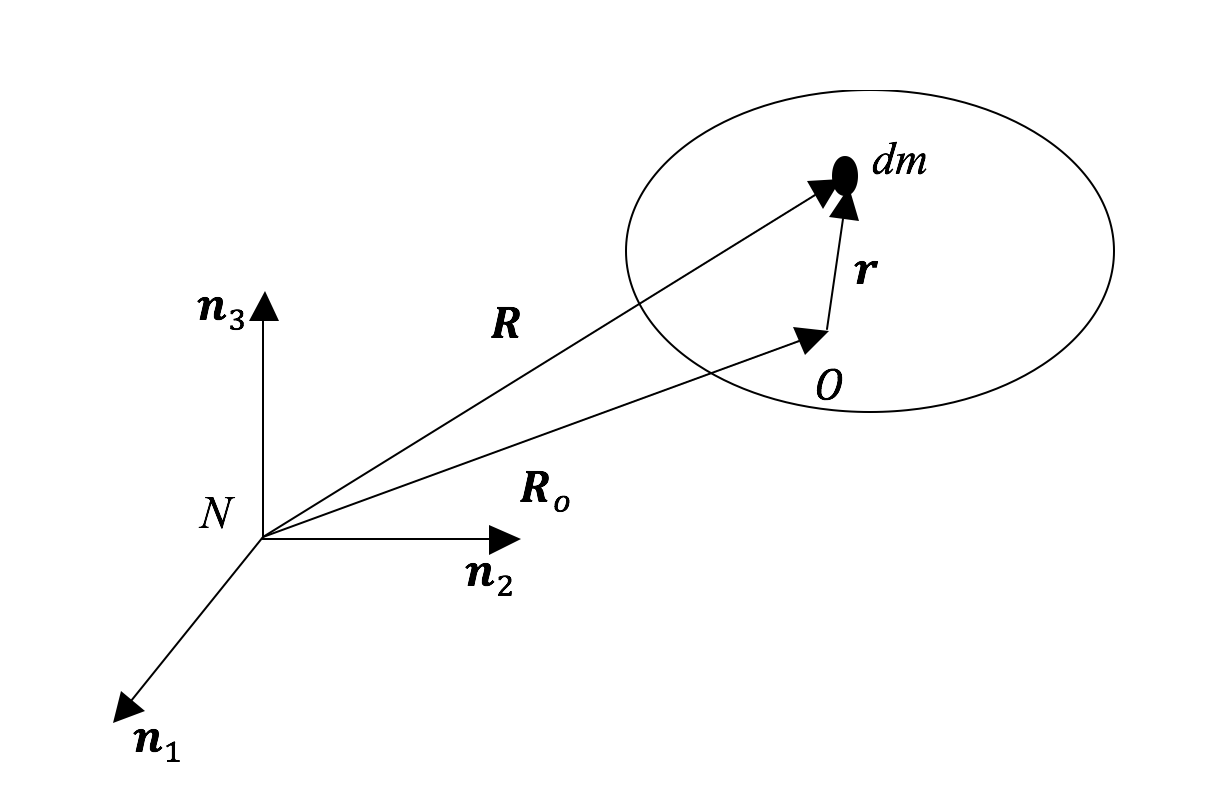
\includegraphics[width=9cm]{figures/attDyn1}    % The printed column width is 8.4 cm.
\caption{Rigid body rotating about an arbitrary point O, given in the N frame} 
\label{fig:attDyn1}
\end{center}
\end{figure}

\begin{figure}
\begin{center}
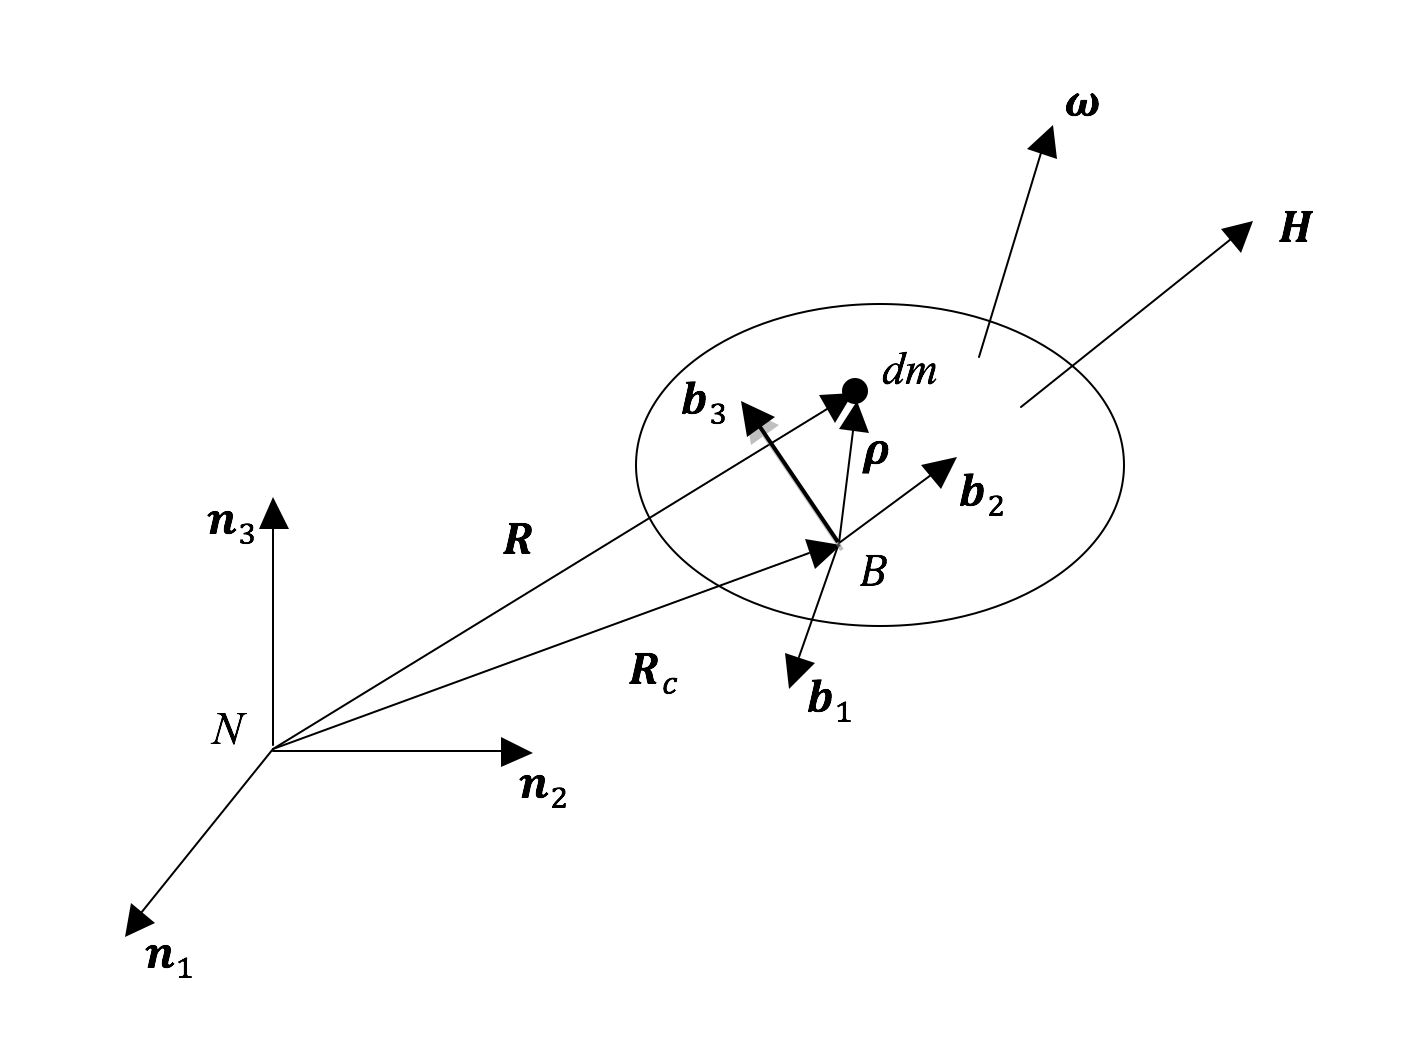
\includegraphics[width=10cm]{figures/attDyn2}    % The printed column width is 8.4 cm.
\caption{Body frame B attached to the rigid body, given in the inertial frame N} 
\label{fig:attDyn2}
\end{center}
\end{figure}

Now, let us take a body fixed frame B with origin at the center of mass of the rigid body as shown in Fig. \ref{fig:attDyn2}. 
In Fig. \ref{fig:attDyn2}, $\bm{\rho}$  is the position vector of $dm$ mass with respect to center of mass of the rigid body, $\bm{R}_c$ is the position vector of the center of mass of the rigid body with respect to the origin of the inertial frame N, and $\bm{R}$ is the position vector of $dm$ with respect to the origin of the inertial frame N. 

The angular velocity of the rigid body in the inertial frame N is denoted as $\bm{\omega} \equiv \bm{\omega}_B^{B/N}$. 
It represents the angular velocity of the body frame B with respect to inertial frame N given in the body frame B. 
Angular momentum vector $\bm{H}$ of a rigid body about its center of mass is given by :

\begin{equation}{\label{eqn:kinematicEquDQM}}
\bm{H} = \int \bm{\rho} \times \dot{\bm{R}} dm
\end{equation}

Since $\bm{R}_C$ is constant

\begin{equation}{\label{eqn:kinematicEquDQM}}
\dot{\bm{R}} = \dot{\bm{R}}_C + \dot{\bm{\rho}} = \dot{\bm{\rho}}
\end{equation}

And from rigidity of the body,

\begin{equation}{\label{eqn:kinematicEquDQM}}
\dot{\bm{\rho}} \equiv \bigg\{ \frac{d\bm{\rho}}{dt} \bigg\}_N = {\cancel{\bigg\{ \frac{d\bm{\rho}}{dt} \bigg\}}}_B + \bm{\omega} \times \bm{\rho} = \bm{\omega} \times \bm{\rho}
\end{equation}

Then, the angular momentum is given as :

\begin{equation}{\label{eqn:kinematicEquDQM}}
\bm{H} = \int \bm{\rho} \times \dot{\bm{R}} dm = \int \bm{\rho} \times \dot{\bm{\rho}} dm = \int \bm{\rho} \times  (\bm{\omega} \times \bm{\rho} )dm
\end{equation}

The components of $\bm{\rho}$ and $\bm{\omega}$ in the body frame B are written as;

\begin{align}{\label{eqn:omega_and_rho}}
\begin{split}
\bm{\rho} & = \rho_1 \bm{b}_1 + \rho_2 \bm{b}_2 + \rho_3 \bm{b}_3 \\
\bm{\omega} & = \omega_1 \bm{b}_1 + \omega_2 \bm{b}_2 + \omega_3 \bm{b}_3 \\
\end{split}
\end{align}

Then, the angular momentum can be written as;

\begin{equation}{\label{eqn:angMomentumComp}}
\bm{H} = H_1 \bm{b}_1 + H_2 \bm{b}_2 + H_3 \bm{b}_3 
\end{equation}

where

\begin{align}{\label{eqn:angularMomentum1}}
\begin{split}
H_1 & = I_{11} \omega_1 + I_{12} \omega_2 + I_{13} \omega_3 \\
H_2 & = I_{21} \omega_1 + I_{22} \omega_2 + I_{23} \omega_3 \\
H_3 & = I_{31} \omega_1 + I_{32} \omega_2 + I_{33} \omega_3 \\
\end{split}
\end{align}

Writing in matrix form gives,

\begin{equation}{\label{eqn:angularMomentumInMatrixForm}}
\begin{bmatrix}
H_1\\[0.2em]
H_2\\[0.2em]
H_3\\[0.2em]
\end{bmatrix}
 =\,
\begin{bmatrix}
I_{11} & I_{12} & I_{13} \\[0.2em]
I_{21} & I_{22} & I_{23} \\[0.2em]
I_{31} & I_{32} &I_{33} \\[0.2em]
\end{bmatrix}
\,
\begin{bmatrix}
\omega_1\\[0.2em]
\omega_2\\[0.2em]
\omega_3\\[0.2em]
\end{bmatrix}
\end{equation}

and in a compact form

\begin{equation}{\label{eqn:angMomentumComp2}}
\bm{H} = \bm{I} \bm{\omega}
\end{equation}

where $\bm{I}$  is called the inertia matrix of the rigid body about a body fixed reference frame B with origin at the center of mass of the rigid body.

Let us write a set of axes to achieve all the products of inertia, or all the elements of the inertia matrix except diagonal elements, are zero. 
This set is called the principal axes and the moments of inertia are called the principal moments of inertia. 
Assuming the axes of the body reference frame B are the principal axes, then the equation for the angular momentum becomes;

\begin{equation}{\label{eqn:angularMomentumInPrincipleAxes}}
\begin{bmatrix}
H_1\\[0.2em]
H_2\\[0.2em]
H_3\\[0.2em]
\end{bmatrix}
 =\,
\begin{bmatrix}
I_{11} & 0 & 0 \\[0.2em]
0 & I_{22} & 0 \\[0.2em]
0 & 0 &I_{33} \\[0.2em]
\end{bmatrix}
\,
\begin{bmatrix}
\omega_1\\[0.2em]
\omega_2\\[0.2em]
\omega_3\\[0.2em]
\end{bmatrix}
\end{equation}

Now, it is time to express the rotational equations of motion - also  known as Euler's equations of motion - for a rigid body.  Remember the angular momentum equation

\begin{equation}{\label{eqn:angMomentumComp}}
\bm{M} = \dot{\bm{H}} 
\end{equation}

where $\bm{H}$ is the angular momentum vector of the rigid body about its center of mass and  $\bm{M}$ is the external moment acting on the rigid body about its center of mass.  We can also write it as;

\begin{equation}{\label{eqn:attDynDerivation1}}
\dot{\bm{H}} = \bigg\{ \frac{d\bm{H}}{dt} \bigg\}_N 
=\,
\bigg\{ \frac{d\bm{H}}{dt} \bigg\}_B  + \bm{\omega}_B^{B/N} \times \bm{H}
 =\,
  \bm{M}
\end{equation}

By taking the time derivative of Eq. \ref{eqn:angMomentumComp2}, assuming the inertia is not dependent on time, and evaluating in  Eq. \ref{eqn:attDynDerivation1}, Euler's rotational equation of motion can be written as 

\begin{empheq}[box=\fbox]{equation}{\label{eqn:attitudeDynamics}}
\dot{\bm{\omega}}_B^{B/N}  = \bm{I}_B^{-1} (\bm{M}_B - \bm{\omega}_B^{B/N} \times \bm{I}_B \bm{\omega}_B^{B/N}) 
\end{empheq}

\section{Translation modeling}

The movement of any object can be represented by changes in its location (translation) or changes in its attitude (rotation) or a combination of both. 
Studying aircraft motion is complicated since those two motions are coupled, e.g a rotation might cause a change in aerodynamic forces which affects the translation. 
Thus, to ease the modeling process, the aircraft is assumed to be a point mass, all its mass collected at its center of gravity, while it translates from one point to the other.
Then, the motion of the that point, at its center of gravity, is described by Newton's laws of motion.
The translations are in direct response to external forces, namely the lift, drag, thrust and weight.
Unfortunately some of those forces depend on the attitude of the aircraft.

\subsection{Translational kinematics}

Time change of the position of the aircraft $\bm{x}_N$ expressed in the navigation frame can be written in terms of translational velocity $\bm{v}_B$ expressed in the body frame as

\begin{align}{\label{eqn:translationalKinematics1}}
\begin{split}
\dot{\bm{x}}_N & = \frac{d}{dt} \big( \bm{x}_N \big) \\
                        & = \frac{d}{dt} \big(\bm{C}_B^N \bm{x}_B \big) \\
                        & = \dot{\bm{C}}_B^N \bm{x}_B + \bm{C}_B^N  \dot{\bm{x}}_B \\
                        & = \bm{C}_B^N \bm{v}_B
\end{split}
\end{align}

using $\bm{x}_B=0$. Eq. \ref{eqn:translationalKinematics1} can also be written as : 

\begin{empheq}[box=\fbox]{equation}{\label{eqn:angularMomentumInPrincipleAxes}}
\begin{bmatrix}
\dot{x}_n\\[0.2em]
\dot{x}_e\\[0.2em]
\dot{x}_d\\[0.2em]
\end{bmatrix}
 =\,
\bm{C}_B^N
\,
\begin{bmatrix}
u\\[0.2em]
v\\[0.2em]
w\\[0.2em]
\end{bmatrix}
\end{empheq}

where, $\bm{v}_B = [u \quad v \quad w]^T$ is the inertial velocity of the center of mass of the body expressed in the body frame $B$ and $\dot{\bm{x}}_N = [\dot{x}_n \quad  \dot{x}_e \quad \dot{x}_d]^T$ is the ground speed vector expressed in the navigation frame $N$. $N$ is assumed to be a local inertial frame.
As mentioned before, the sequence of the transformation between frames effects the final transformation matrix so does the attitude kinematic equations. 
In the course of the study, the sequence is assumed to be yaw - pitch - roll and the corresponding transformation matrix from the navigation frame to body-fixed frame is given in Eq. ~\ref{eqn:C_NtoB}.

\begin{equation}{\label{eqn:C_NtoB}}
C_N^B
= \,
\begin{bmatrix}
1 - 2(q_2^2 + q_3^2) & 2(q_1 q_2 + q_0 q_3) & 2(q_1 q_3 - q_0 q_2)  \\[0.2em]
2(q_1 q_2 - q_0 q_3) & 1 - 2(q_1^2 + q_3^2) & 2(q_2 q_3 + q_0 q_1)\\[0.2em]
2(q_1 q_3 + q_0 q_2) & 2(q_2 q_3 - q_0 q_1) & 1 - 2(q_1^2 + q_2^2) \\[0.2em]
\end{bmatrix}
\end{equation}


\subsection{Translational dynamics}

The aircraft is assumed to be a point mass, all its mass collected at its center of gravity, while it translates from one point to an other.
Then, the motion of that point is described by Newton's laws of motion.
The translations are in direct response to external forces, namely the lift, drag, thrust and weight.
From now on, the aircraft will be assumed to be flying over a small region compared to size of the Earth so that the Earth is locally flat to neglect centripetal acceleration (due to Earth's curvature). 
Another assumption is that the frame attached to Earth being an inertial frame by ignoring Coriolis acceleration so that Newton's laws apply. 

\begin{equation}{\label{eqn:newtonsSecondLaw}}
\sum_j \bm{F}_j = \left. \frac{d}{dt} \big( m \bm{v} \big) \right|_I
\end{equation}

Unfortunately, those forces that directly effect the translation depend on the attitude of the aircraft, complicating the dynamics.

Here, the subscript $I$ represents the frame in which the time derivation occurs, which is an inertial frame in this case. 
To represent time derivation in the inertial frame in terms of time derivation in body frame, relative rotation of the body frame with respect to the inertial frame should be included such that


\begin{equation}{\label{eqn:newtonsDerivationFrameDependency}}
\left. \frac{d}{dt} \big( m \bm{v} \big) \right|_I = \left. \frac{d}{dt} \big( m \bm{v} \big) \right|_B + \bm{\omega}^{B/I} \times \big( m\bm{v} \big)
\end{equation}

Substituting Eq. ~\ref{eqn:newtonsDerivationFrameDependency} in Eq. ~\ref{eqn:newtonsSecondLaw} and then projecting the vector variables in the body frame as well as assuming mass is constant gives


 \begin{equation}{\label{eqn:newtonsSecondLaw2}}
\frac{1}{m} \bigg( \sum_j \bm{F}_{B_j} \bigg)= \left. \frac{d\big(\bm{v}_B \big)}{dt}  \right|_B + \bm{\omega}_B^{B/I} \times \bm{v}_B
\end{equation}

Writing the summation of forces in terms of the forces acting on the aircraft :

\begin{equation}{\label{eqn:dynamicsEquation1}}
\frac{1}{m} \Big( m \bm{g}_B + \bm{F}_{{thrust}_B} + \bm{F}_{{aero}_B} \Big)  =\,
\begin{bmatrix}
\dot{u}\\[0.2em]
\dot{v}\\[0.2em]
\dot{w}\\[0.2em]
\end{bmatrix}
+\,
\begin{bmatrix}
p\\[0.2em]
q\\[0.2em]
r\\[0.2em]
\end{bmatrix}
\times \,
\begin{bmatrix}
u\\[0.2em]
v\\[0.2em]
w\\[0.2em]
\end{bmatrix}
\end{equation}

Rearranging terms and writing the forces in more detail gives :

\begin{empheq}[box=\fbox]{equation}{\label{eqn:dynamicsEquation2}}
\begin{bmatrix}
\dot{u}\\[0.2em]
\dot{v}\\[0.2em]
\dot{w}\\[0.2em]
\end{bmatrix}
=\,
\begin{bmatrix}
{-g \sin{\theta}}\\[0.2em]
{g \sin{\phi} \cos{\theta} }\\[0.2em]
{g \cos{\phi} \cos{\theta}}\\[0.2em]
\end{bmatrix}
+\,
\frac{1}{m}
\,
\begin{bmatrix}
F_{thrust}\\[0.2em]
0\\[0.2em]
0\\[0.2em]
\end{bmatrix}
+\,
\frac{1}{m}
\,
\begin{bmatrix}
X^b\\[0.2em]
Y^b\\[0.2em]
Z^b\\[0.2em]
\end{bmatrix}
-\,
\begin{bmatrix}
qw-rv\\[0.2em]
ru-pw\\[0.2em]
pv-qu\\[0.2em]
\end{bmatrix}
\end{empheq}

which are the equations of motion of the aircraft. 

\section{Drone model}

The calculation of aerodynamic forces and moments that are necessary to solve the equations of motion of a drone will be given in this section. 
During the course of this PhD, two kind of drones have been simulated : a drone from ETH university \cite{ducard2009fault} and MAKO (used in drone lab) given in Fig.~\ref{figure:mako}. 
ETH drone has 2 ailerons, 2 elevators and a rudder as its control surfaces, while MAKO has only 2 control surfaces: elevons. 
An example of an elevon can be seen in the schematic of Zagi given in Fig.~\ref{fig:bodyNEDframes}. 
Changed in the same direction, elevons are used as an elevators (changes the pitch) while changed in reverse direction, they act as ailerons (changes the roll). 

\begin{figure}
\begin{center}
%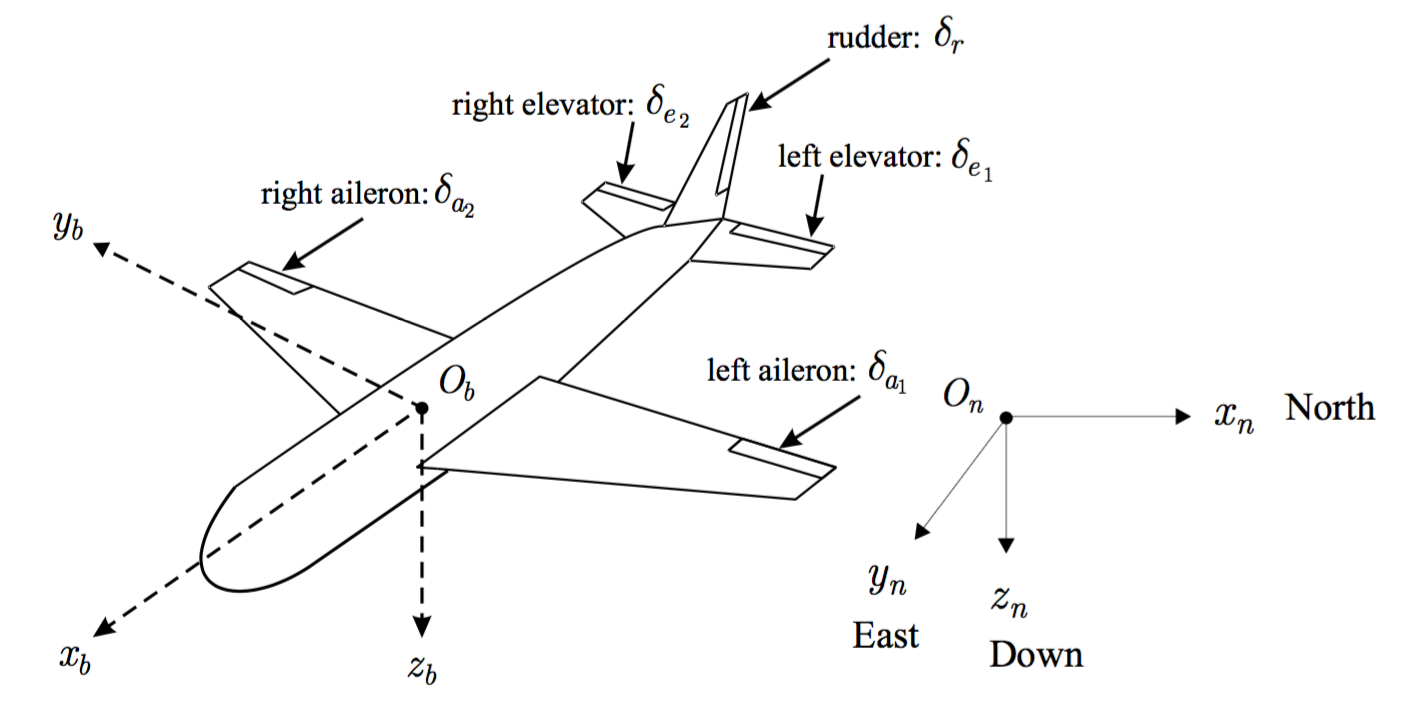
\includegraphics[width=11cm]{figures/bodyNEDframes}    % The printed column width is 8.4 cm.
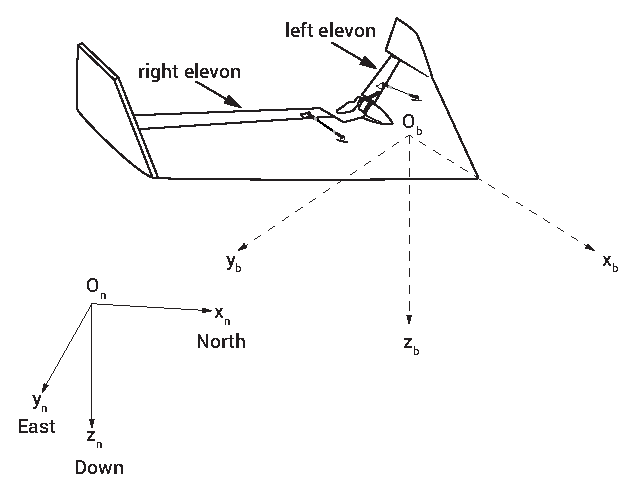
\includegraphics[width=13cm]{figures/ZagiElevon}    % The printed column width is 8.4 cm.
\caption{Body fixed frame and North East Down (NED) frame representations} 
\label{fig:bodyNEDframes}
\end{center}
\end{figure}

First, to calculate the moments of inertia of MAKO, it is hanged by two strings, at different orientations, as shown in Fig.~\ref{fig:inertia}, and measurements performed by timing the oscillation period for each axis. 
The resultant moment of inertias are given Table~\ref{arm:MAKOspecs}. 

\begin{figure}
\centering
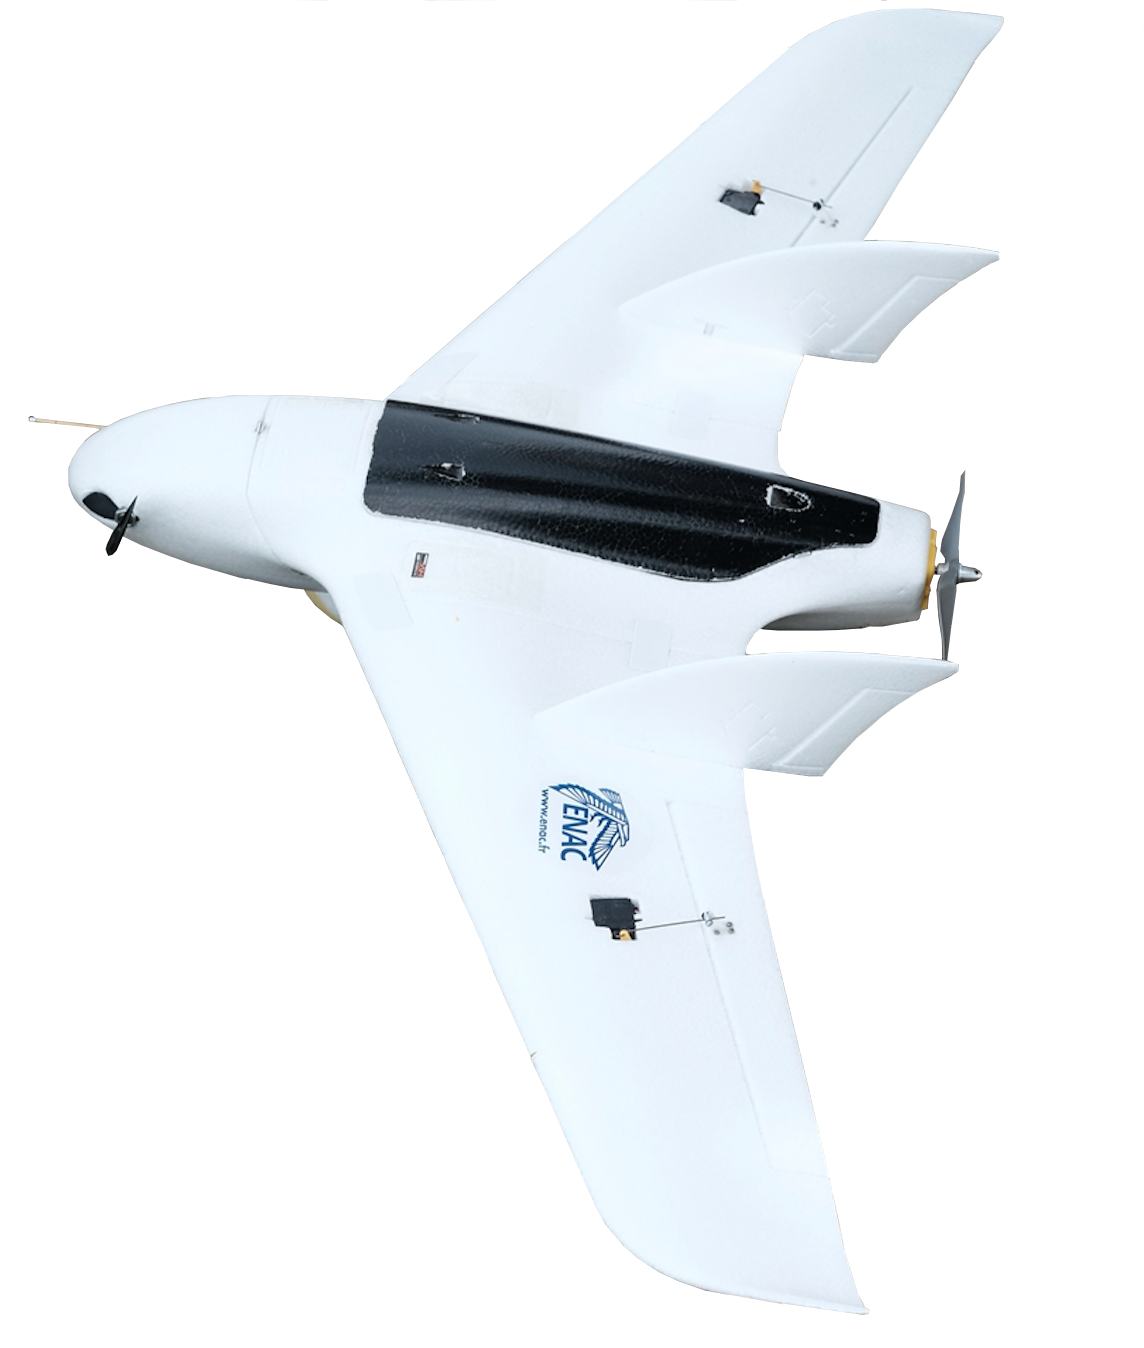
\includegraphics[width=0.7\columnwidth]{figures/makoEmptyBack}
\caption{MAKO}
\label{figure:mako}
\end{figure}

 \begin{figure*}
      \centering
      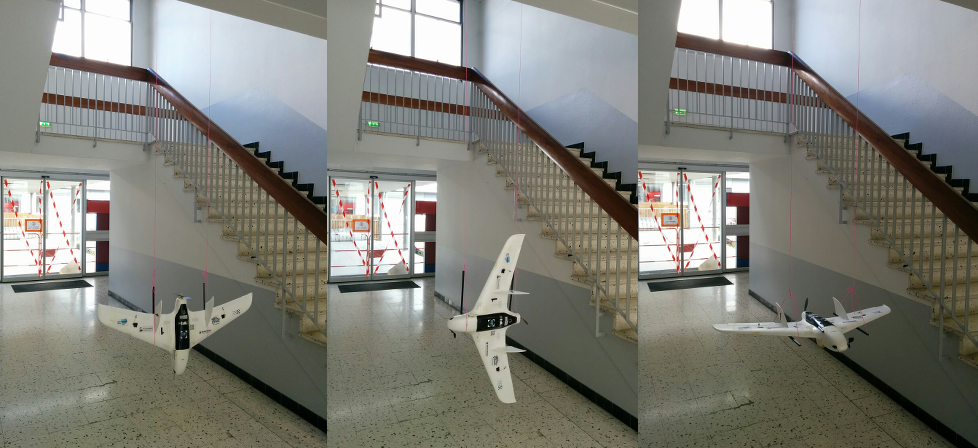
\includegraphics[width=0.9\textwidth]{figures/Mako_Inertia_combined_small.png}
      \caption{Moments of inertia measurements for each axis, $I_{xx} , I_{yy} , I_{zz} $.}
      \label{fig:inertia}
 \end{figure*}
 
 \begin{table}
\caption{General specifications of MAKO \cite{bronz2016aerodynamic}}
\label{arm:MAKOspecs}
\begin{center}
\begin{tabular}{ ||p{4cm}|p{3cm}|p{2cm}||}\hline
\textbf{Parameter} & \textbf{Value} & \textbf{Definition} \\\hline
Wing span (b)                  & $\ \ \, 1.288 $	   & $[m]$ \\\hline
Wing surface area (S)      & $ \ \ \, 0.27 $           &  $[m^2]$ \\\hline
Mean aero chord ($\bar{c}$)         & $\ \ \, 0.21$           & $[m]$ \\\hline
Take-off mass (m)             & $\ \ \, 0.7 - 2.0$       & $[kg]$ \\\hline
Flight velocity           & $\ \ \, 10 - 25$       & $[m/s]$ \\\hline
$I_{xx}$                         & $\ \ \, 0.02471284$   & $[kg \cdot m^2]$ \\\hline
$I_{yy}$                         & $\ \ \, 0.015835159$   & $[kg \cdot m^2]$ \\\hline
$I_{zz}$                         & $\ \ \, 0.037424499$   & $[kg \cdot m^2]$ \\\hline
\end{tabular}
\end{center}
\end{table}

 \begin{table}
\caption{Parameters of ETH drone \cite{bronz2016aerodynamic}}
\label{arm:ethDrone}
\begin{center}
\begin{tabular}{ ||p{6cm}|p{3cm}|p{2cm}||}\hline
\textbf{Parameter} & \textbf{Value} & \textbf{Definition} \\\hline
Wing span (b)                & $\ \ \, 3.1 $	   & $[m]$ \\\hline
Wing surface area (S)      & $ \ \ \, 1.80$           &  $[m^2]$ \\\hline
Mean aero chord ($\bar{c}$)          & $\ \ \, 0.58$           & $[m]$ \\\hline
Take-off mass (m)             & $\ \ \, 28$       & $[kg]$ \\\hline
Propeller diameter (D)           & $\ \ \, 28$       & $[m]$ \\\hline
time constant of the engine ($\tau_n$)           & $\ \ \, 28$       & $[m]$ \\\hline
$I_{xx}$                         & $\ \ \, 2.56$   & $[kg \cdot m^2]$ \\\hline
$I_{yy}$                         & $\ \ \, 10.9$   & $[kg \cdot m^2]$ \\\hline
$I_{zz}$                         & $\ \ \, 11.3$   & $[kg \cdot m^2]$ \\\hline
$I_{zx}$                         & $\ \ \, 0.5$   & $[kg \cdot m^2]$ \\\hline
$I_{xz}$                         & $\ \ \, 0.5$   & $[kg \cdot m^2]$ \\\hline
\end{tabular}
\end{center}
\end{table}

\subsection{Modeling of aerodynamic moments}

The attitude of the aircraft changes with the torques applied to the airframe. 

\begin{equation}{\label{eqn:torqueTotal}}
\bm{M}_B
= \,
\begin{bmatrix}
L_{b} \\
M_{b}\\
N_{b}\\
\end{bmatrix}
\end{equation}

Here, $L_b$ is the roll torque, $M_b$ is the pitch torque, and $N_b$ is the yaw torque given in body frame shown in Fig.~\ref{fig:bodyNEDframes}.

The stability derivatives required to calculate the moments are given under Table~\ref{arm:ethcraftStabilityDeriv} for ETH drone and under Table~\ref{arm:MAKOstabilityDeriv} for MAKO. 
Those values for ETH drone are taken from \cite{ducard2009fault} while for MAKO they are calculated via AVL. 
AVL is an open source program developed at MIT and uses vortex-lattice method for the aerodynamic and stability calculations.
The output of the program is linearized at a selected trim condition, therefore all the coefficients are calculated around the equilibrium point at $14m/s$ cruise flight condition.
The center of gravity is located at $X_{CG}= 0.295\,m$, which corresponds to a $8\,\%$ of positive static margin that has been flight tested. %FIXME we have to check if we used modified AVL with viscous add-on or not...

\subsubsection{Roll torque}

Roll torque is given as a multiplication of dynamic pressure $\bar{q}$, wing surface area $S$, wingspan $b$,  and dimensionless roll torque $C_L$ as :

\begin{equation}{\label{eqn:rollTorque}}
L_B = \bar{q} \, S \, b \, C_L
\end{equation}

Here, the dynamic pressure is calculated as :

\begin{equation}{\label{eqn:dynamicPressure}}
\bar{q}=\frac{\rho V_T^2}{2} 
\end{equation}

while the air density $\rho$ is given by the international standard atmosphere model for low altitude (<11000m) as :

\begin{equation}{\label{eqn:airDensityStandard}}
\rho = \frac{p_0 \Big[ 1+\frac{ah}{T_0} \Big]^{5.2561}}{R\,T}
\end{equation}

where the temperature $T$ is given as

\begin{equation}{\label{eqn:temperature}}
T=T_0\Big[ 1 + \frac{ah}{T_0} \Big]
\end{equation}

with $T_0=288.15K$, $a = -6.5 \times 10^{-3} \, K/m$, $R=287.3\;m^2K^{-1}s^{-2}$ and $p_0=1013 \times 10^2 \;Nm^{-2}$.

Next, is to calculate the dimensionless roll torque in Equ.~\ref{eqn:rollTorque}.
For ETH drone, it is given by \cite{stevens2015aircraft,ducard2009fault,mockli2006guidance} :

\begin{table}
\label{arm:momentsETHcraft}
\caption{Stability derivatives for ETH UAV \cite{ducard2009fault}}
\label{arm:ethcraftStabilityDeriv}
\begin{center}
\begin{tabular}{ ||p{3cm}|p{3cm}|p{3cm}||}\hline
\textbf{Parameter} & \textbf{Value} & \textbf{Definition} \\\hline
$C_{L_{a1}} = - C_{L_{a2}}$ & $-3.395 \times 10^{-2}$	   & roll derivative \\\hline
$C_{L_{e1}} = - C_{L_{e2}}$ & $-0.485 \times 10^{-2}$         & roll derivative \\\hline
$C_{L_{\tilde{p}}}$                 & $-1.92 \times 10^{-1}$	   & roll derivative \\\hline
$C_{L_{\tilde{r}}} $                 & $\ \ \, 3.61 \times 10^{-2}$     & roll derivative \\\hline
$C_{L_\beta}$                        & $-1.30 \times 10^{-2}$	   & roll derivative \\\hline
$ C_{M_{1}}$                          & $\ \ \, 2.08 \times 10^{-2}$	   & pitch derivative \\\hline
$C_{M_{a1}} = C_{M_{a2}} $ & $\ \ \, 0.389 \times 10^{-1}$  & pitch derivative \\\hline
$C_{M_{e1}} = C_{M_{e2}} $ & $\ \ \, 2.725 \times 10^{-1}$  &  pitch derivative \\\hline
$C_{M_{\tilde{q}}} $               & $-9.83$	                            & pitch derivative \\\hline
$C_{M_\alpha} $                    & $-9.03 \times 10^{-2}$ 	   & pitch derivative \\\hline
$C_{N_{\delta r}}$                  & $\ \ \, 5.34 \times 10^{-2}$ 	   & yaw derivative \\\hline
$ C_{N_{\tilde{r}}}$                 & $-2.14 \times 10^{-1}$	   & yaw derivative \\\hline
$C_{N_\beta} $                       & $\ \ \, 8.67 \times 10^{-2}$	     & yaw derivative \\\hline
\end{tabular}
\end{center}
\end{table}

\begin{table}
\label{arm:momentsMAKO}
\caption{Stability derivatives for MAKO extracted from AVL program at $14 m/s$ equilibrium cruise speed \cite{bronz2016aerodynamic}}
\label{arm:MAKOstabilityDeriv}
\begin{center}
\begin{tabular}{ ||p{3cm}|p{3cm}|p{3cm}||}\hline
\textbf{Parameter} & \textbf{Value} & \textbf{Definition} \\\hline
$C_{L_a}$                             & $-0.1956 \times 10^{-2}$	   & roll derivative \\\hline
$C_{L_{\tilde{p}}}$                 & $-4.095 \times 10^{-1}$	   & roll derivative \\\hline
$C_{L_{\tilde{r}}} $                 & $\ \ \, 6.203 \times 10^{-2}$     & roll derivative \\\hline
$C_{L_\beta}$                        & $\ \ \, 3.319 \times 10^{-2}$	   & roll derivative \\\hline
$C_{M_0}$ 			     & $\ \ \, 0$  &  pitch derivative \\\hline
$C_{M_e}$ 			     & $-0.076 \times 10^{-1}$  &  pitch derivative \\\hline
$C_{M_{\tilde{q}}} $               & $-1.6834$	                            & pitch derivative \\\hline
$C_{M_\alpha} $                    & $-32.34 \times 10^{-2}$ 	   & pitch derivative \\\hline
$C_{N_0}$                             & $\ \ \, 0$              	   & yaw derivative \\\hline
$C_{N_a}$                             & $-0.0126 \times 10^{-2}$	   & yaw derivative \\\hline
$C_{N_{\tilde{p}}}$                 & $-4.139 \times 10^{-2}$ 	   & yaw derivative \\\hline
$C_{N_{\tilde{r}}}$                 & $-0.1002 \times 10^{-1}$	   & yaw derivative \\\hline
$C_{N_\beta} $                      & $\ \ \, 2.28 \times 10^{-2}$	   & yaw derivative \\\hline
\end{tabular}
\end{center}
\end{table}

\begin{equation}{\label{eqn:bigCraftC_L}}
C_L = C_{L_{a1}} \, \delta_{a1} + C_{L_{a2}} \, \delta_{a2} + C_{L_{e1}} \, \delta_{e1} + C_{L_{e2}} \, \delta_{e2} + C_{L_{\tilde{p}}} \, \tilde{p} + C_{L_{\tilde{r}}} \, \tilde{r} +  C_{L_\beta} \, \beta 
\end{equation}

For MAKO, the dimensionless roll torque is given by :

\begin{equation}{\label{eqn:makoC_L}}
C_L = C_{L_{a}} \, \delta_{a} + C_{L_{\tilde{p}}} \, \tilde{p} + C_{L_{\tilde{r}}} \, \tilde{r} +  C_{L_\beta} \, \beta 
\end{equation}

where $\delta_{a1},\,\delta_{a2}$ are the aileron deflections, $\delta_{e1},\, \delta_{e2}$ are the elevator deflections, $\delta_a$ is the aileron deflection for MAKO, $\beta$ is the sideslip angle representing the angle between airspeed vector $\bm{V_T}$ and the projection of $\bm{V_T}$ onto $x_b-z_b$ plane as shown in Fig.~\ref{fig:windFrame} and given as :

\begin{equation}{\label{eqn:sideslipAngle}}
\beta = \arcsin{\frac{v_T}{V_T}}
\end{equation}

$\tilde{p}, \tilde{r}$ are dimensionless angular rates given by :

 \begin{equation}{\label{eqn:dimensionlessAngularVelocties}}
\tilde{p}=\frac{bp}{2V_T} \qquad \tilde{r}=\frac{br}{2V_T}
\end{equation}

Here, $b$ is the wingspan, $p,q$ are angular rates and $V_T$ is the norm of the airspeed vector such as :

\begin{equation}{\label{eqn:airspeedVector}}
V_T=\sqrt{u_T^2 + v_T^2 + w_T^2}
\end{equation}

Airflow acting on the aircraft is described by airspeed vector $\bm{V_T}$ (see Fig.~\ref{fig:windFrame}). The wind frame is shown in Fig.~\ref{fig:windFrame} with axes $(x_w, y_w, z_w)$ where $x_w$ points along the airspeed vector $\bm{V}_T$.
Airspeed vector in terms of its components in body frame, and in wind frame can be given as

\begin{figure}
\begin{center}
%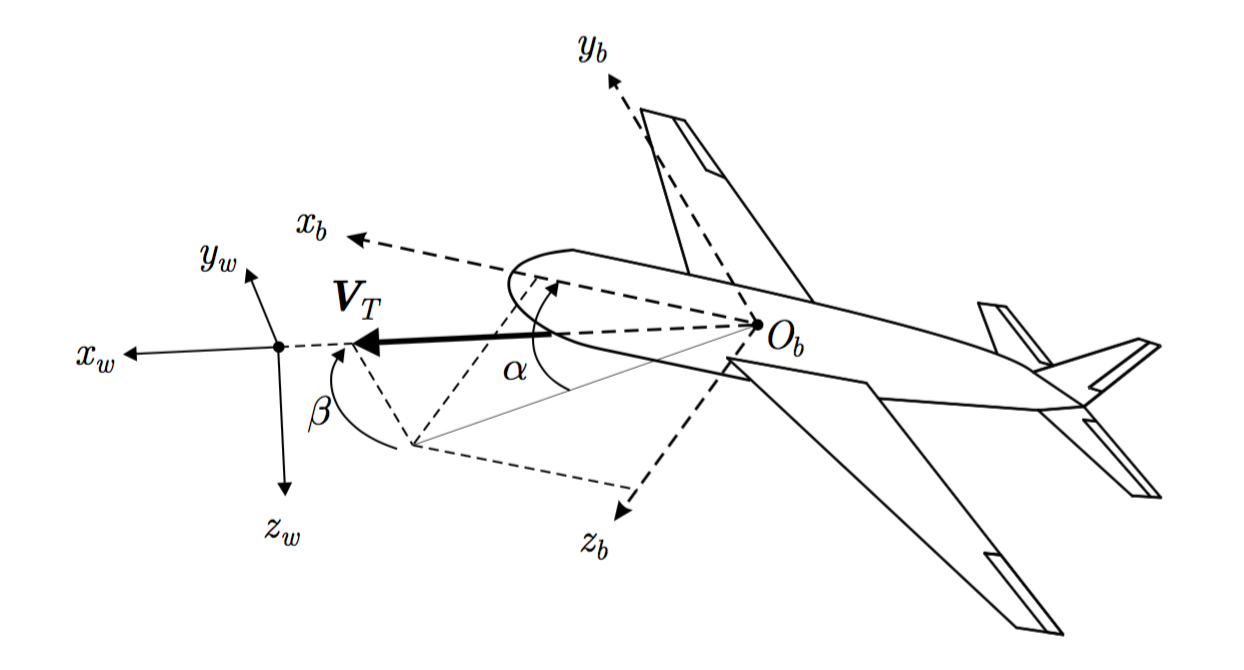
\includegraphics[width=11cm]{figures/windFrame}    % The printed column width is 8.4 cm.
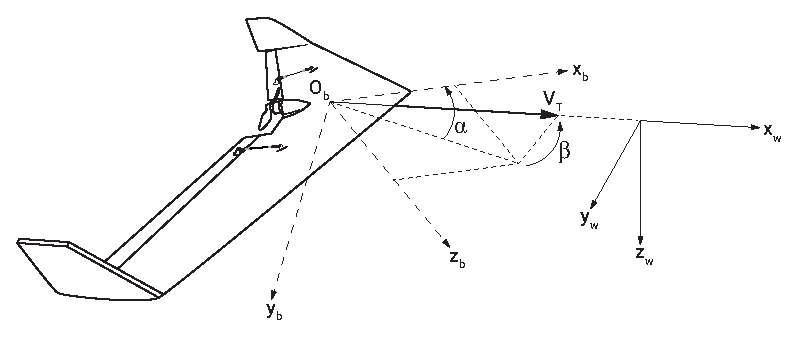
\includegraphics[width=15cm]{figures/ZagiWindframe}    % The printed column width is 8.4 cm.
\caption{Wind frame, airspeed vector $\bm{V}_T$, angle of attack $\alpha$ and side slip angle $\beta$ representation \cite{ducard2009fault}} 
\label{fig:windFrame}
\end{center}
\end{figure}

\begin{equation}{\label{eqn:airspeedComponents}}
\bm{V}_{\bm{T}_B}
=\,
\begin{bmatrix}
u_{T} \\
v_{T}\\
w_{T}\\
\end{bmatrix}
\qquad \,
\bm{V}_{\bm{T}_W}
=\,
\begin{bmatrix}
V_{T} \\
0\\
0\\
\end{bmatrix}
\end{equation}

The relationship between $\bm{V}_{\bm{T}_B}$ and $\bm{V}_{\bm{T}_W}$ can be written as \cite{ducard2009fault}:

\begin{equation}{\label{eqn:airspeedVectorTransformation}}
\bm{V}_{\bm{T}_B}=\bm{C_W^B}\bm{V}_{\bm{T}_W}
\end{equation}

Note that the inertial velocity of the aircraft $\bm{v}_B = {[u \quad v \quad w]}^T$ is different than airspeed vector $\bm{V}_{\bm{T}_B} = {[u_T \quad v_T \quad w_T ]}^T$. 
Those two vectors are related to wind velocity $\bm{W}$ by :

\begin{equation}{\label{eqn:inertialVelocityAirspeedVectorWind}}
\bm{v}=\bm{V_T} + \bm{W}
\end{equation}

When those vectors are projected on to body frame, the relation becomes

\begin{equation}{\label{eqn:inertialVelocityAirspeedVectorWind}}
\bm{v}_B=\bm{V}_{\bm{T}_B} + \bm{C_N^B} \bm{W}_N
\end{equation}

\begin{figure}
\begin{center}
%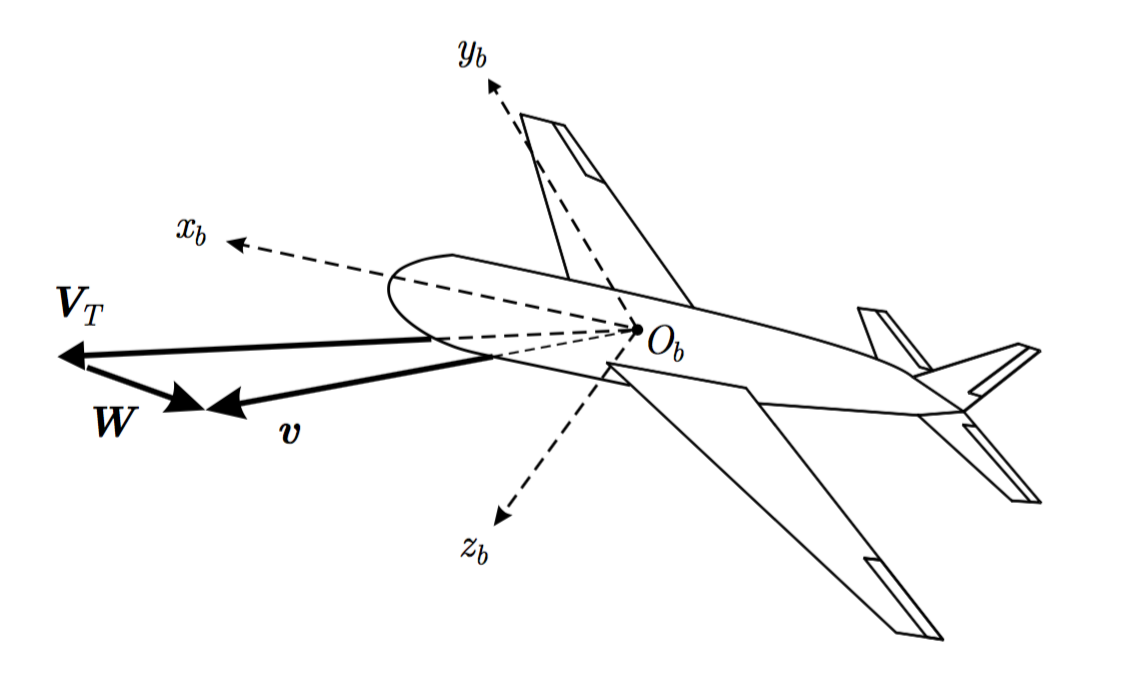
\includegraphics[width=11cm]{figures/windDisturbance}    % The printed column width is 8.4 cm.
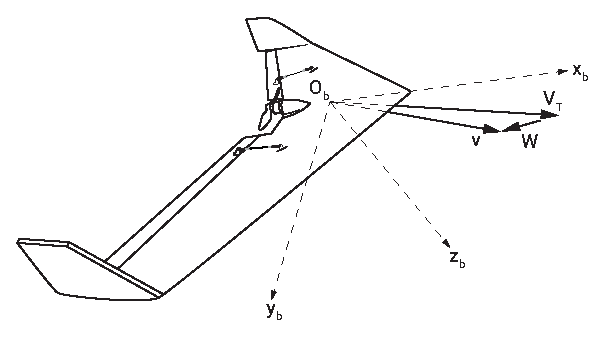
\includegraphics[width=13cm]{figures/ZagiWindDisturbance}    % The printed column width is 8.4 cm.
\caption{Relation revealed between the inertial velocity vector $\bm{v}$, airspeed vector $\bm{V}_T$ and wind disturbance $\bm{W}$ \cite{ducard2009fault}} 
\label{fig:windDisturbance}
\end{center}
\end{figure}

and with components :

\begin{equation}{\label{eqn:inertialVelocityAirspeedVectorWindComponents}}
\begin{bmatrix}
u \\
v\\
w\\
\end{bmatrix}
=\,
\begin{bmatrix}
u_{T} \\
v_{T}\\
w_{T}\\
\end{bmatrix}
+\,
\bm{C_N^B}
\begin{bmatrix}
W_n \\
W_e\\
W_d\\
\end{bmatrix}
\end{equation}


\subsubsection{Pitch torque}

Pitch torque is given as a multiplication of dynamic pressure $\bar{q}$, wing surface area $S$, mean aero chord $\bar{c}$,  and dimensionless pitch torque $C_M$ as :

\begin{equation}{\label{eqn:pitchTorque}}
M_B = \bar{q} \, S \, \bar{c} \, C_M
\end{equation}

where the dimensionless pitch torque is given as for ETH drone as :

\begin{equation}{\label{eqn:bigCraftC_M}}
C_M = C_{M_{1}} + C_{M_{a1}} \, \delta_{a1} + C_{M_{a2}} \, \delta_{a2} + C_{M_{e1}} \, \delta_{e1} + C_{M_{e2}} \, \delta_{e2} + C_{M_{\tilde{q}}} \, \tilde{q} +  C_{M_\alpha} \, \alpha 
\end{equation}

and for MAKO :

\begin{equation}{\label{eqn:makoC_M}}
C_M =  C_{M_{0}} + C_{M_{e}} \, \delta_{e} + C_{M_{\tilde{q}}} \, \tilde{q} +  C_{M_\alpha} \, \alpha 
\end{equation}

where the variables not introduced up to now are the dimensionless roll rate $\tilde{q}$, elevator deflection $\delta_{e}$ and angle of attack $\alpha$. Angle of attack $\alpha$ is defined as the angle between the projection of the airspeed vector $\bm{V_T}$ onto the $x_b-z_b$ plane and $x_b$ axis as can be seen in Fig.~\ref{fig:windFrame}, and calculated as :

\begin{equation}{\label{eqn:angleOfAttack}}
\alpha = \arctan{\Big( \frac{w_T}{u_T} \Big)}
\end{equation}

\subsubsection{Yaw torque}

Yaw torque can be given as

\begin{equation}{\label{eqn:yawTorque}}
N_B = \bar{q} \, S \, b \, C_N \\
\end{equation}

with a dimensionless yaw torque for the ETH drone : 

\begin{equation}{\label{eqn:bigCraftC_N}}
C_N= C_{N_{\delta r}} \, \delta_{r} + C_{N_{\tilde{r}}} \, \tilde{r} +  C_{N_\beta} \, \beta 
\end{equation}

and for the MAKO :

\begin{equation}{\label{eqn:makoC_N}}
C_N= C_{N_{0}} + C_{N_{a}} \, \delta_{a} + C_{N_{\tilde{p}}} \, \tilde{p} + C_{N_{\tilde{r}}} \, \tilde{r} +  C_{N_\beta} \, \beta 
\end{equation}

where $\bar{q}$ is the dynamic pressure, $V_T$ is the total airspeed of the aircraft, $\rho$ is the air density, $S$ is the wing total surface, $b$ is the wing span, and $\bar{c}$ mean aerodynamic wing chord. 


\subsection{Modeling of aerodynamic forces}

The position of the aircraft changes with the forces applied to the airframe. The calculation of aerodynamic forces, lift force, drag force, lateral force and thrust force are given below.

%%%% LIFT FORCE %%%%

\subsubsection{Lift force}

The lift force is given in the wind frame as : 

\begin{equation}{\label{eqn:liftForce}}
Z^w = \bar{q} \, S \,  C_Z(\alpha)
\end{equation}

where the dimensionless lift coefficient is calculated as below :

\begin{equation}{\label{eqn:liftCoef}}
C_Z(\alpha) = C_{Z_0} + C_{Z_{\alpha}} \alpha 
\end{equation}


%%%% DRAG FORCE %%%%

\subsubsection{Drag force}

Drag force in the wind frame is calculated as a multiplication of the dynamic pressure, wing surface area, and the drag coefficient as given in Equ.~\ref{eqn:dragForceETHcraft} :

\begin{equation}{\label{eqn:dragForceETHcraft}}
X^w = \bar{q} \, S \,  C_X(\alpha, \beta)
\end{equation}

where the dimensionless drag coefficient for ETH drone is given as :

\begin{equation}{\label{eqn:dragCoeffETHcraft}}
C_X(\alpha, \beta) = C_{X_1} + C_{X_{\alpha}} \alpha + C_{X_{\alpha 2}} {\alpha}^2 + C_{X_{\beta 2}} {\beta}^2 
\end{equation}

While for MAKO the drag force is given by \cite{bronz2016aerodynamic} :

\begin{equation}{\label{eqn:dragForceMAKO}}
X^w = \bar{q} \, S \, C_{Z}(\alpha, \beta)
\end{equation}

and the dimensionless drag coefficient for MAKO \cite{bronz2016aerodynamic} :

\begin{equation}{\label{eqn:dragCoeffMAKO}}
C_X(\alpha) = C_{X_0} + C_{X_k} \, C_Z^2 = C_{X_0} + C_{X_k} \, (C_{Z_0} + C_{Z_{\alpha}} \alpha )^2
\end{equation}

%%%% LATERAL FORCE %%%%

\subsubsection{Lateral force}

The lateral force is given as :

\begin{equation}{\label{eqn:lateralForceETHcraft}}
Y^w = \bar{q} \, S \,  C_Y(\beta)
\end{equation}

where the dimensionless lateral coefficient for ETH drone is given as :

\begin{equation}{\label{eqn:lateralCoeffETHcraft}}
C_Y(\beta) = C_{Y_\beta} \beta
\end{equation}

and for MAKO :

\begin{equation}{\label{eqn:lateralCoeffMAKO}}
C_Y(\beta, \, \tilde{p}, \, \tilde{r}, \, \delta_a) = C_{Y_\beta} \beta + C_{Y_{\tilde{p}}} \, \tilde{p} + C_{Y_{\tilde{r}}} \, \tilde{r} + C_{Y_a} \, \delta_a 
\end{equation}

where the coefficients can be seen in Tables~\ref{arm:forcesETHcraft} and~\ref{arm:forcesMAKO}.

\begin{table}
\caption{Aerodynamic force derivatives for ETH UAV \cite{ducard2009fault}}
\label{arm:forcesETHcraft}
\begin{center}
\begin{tabular}{ ||p{3cm}|p{3cm}|p{4cm}||}\hline
\textbf{Parameter} & \textbf{Value} & \textbf{Definition} \\\hline
$C_{Z_0}$                             & $\ \ \,1.29 \times 10^{-2}$	   & lift derivative \\\hline
$C_{Z_{\alpha}}$                   & $-3.25 $                                 & lift derivative \\\hline
$C_{X_1}$                             & $-2.12 \times 10^{-2}$	   & drag derivative \\\hline
$C_{X_{\alpha}}$                   & $-2.66 \times 10^{-2}$          & drag derivative \\\hline
$C_{X_{\alpha 2}}$                & $-1.55 $	                            & drag derivative \\\hline
$C_{X_{\beta 2}} $                 & $-4.01 \times 10^{-1}$	   & drag derivative \\\hline
$C_{Y_\beta} $                      & $-3.79 \times 10^{-1}$          & side force derivative \\\hline
\end{tabular}
\end{center}
\end{table}


\begin{table}
\caption{Aerodynamic force derivatives for MAKO extracted from AVL program at $14 m/s$ equilibrium cruise speed\cite{bronz2016aerodynamic}}
\label{arm:forcesMAKO}
\begin{center}
\begin{tabular}{ ||p{3cm}|p{3cm}|p{4cm}||}\hline
\textbf{Parameter} & \textbf{Value} & \textbf{Definition} \\\hline
$C_{Z_0}$                             & $-8.53 \times 10^{-2}$	         & lift derivative \\\hline
$C_{Z_{\alpha}}$                   & $\ \ \,3.9444$                               & lift derivative \\\hline
$C_{Z_q}$                             & $\ \ \,4.8198$	       		         & lift derivative \\\hline
$C_{Z_e}$                             & $\ \ \,1.6558 \times 10^{-2}$        & lift derivative \\\hline
$C_{X_0}$                             & $\ \ \, 2.313 \times 10^{-2}$	   & drag derivative \\\hline
$C_{X_k}$                              & $\ \ \, 1.897 \times 10^{-1}$          & drag derivative \\\hline
$C_{Y_\beta}$ 			     & $-2.708 \times 10^{-1}$             & side force derivative \\\hline
$C_{Y_{\tilde{p}}}$                 & $\ \ \, 1.695 \times 10^{-2}$	& side force derivative \\\hline
$C_{Y_{\tilde{r}}}$                  & $\ \ \, 5.003 \times 10^{-2}$ 	& side force derivative \\\hline
$C_{Y_a}$                             & $\ \ \, 0.0254 \times 10^{-2}$	& side force derivative \\\hline
\end{tabular}
\end{center}
\end{table}

%%%% THRUST FORCE %%%%

\subsubsection{Thrust force model}

The thrust generated by the propeller can be written as :

\begin{equation}{\label{eqn:thrustModel}}
F_T = \rho n^2 D^4 C_{F_T}
\end{equation}

where the dimensionless thrust coefficient for ETH drone is calculated as :

\begin{equation}{\label{eqn:thrustETHcraft}}
C_{F_T} = C_{F_{T1}} + C_{F_{T2}} J + C_{F_{T3}} J^2 
\end{equation}

Here, $J$ is the advance ratio, and for ETH drone, it is given by

\begin{equation}{\label{eqn:advRatETHcraft}}
J = \frac{V_T}{n \pi D}
\end{equation}

\begin{table}
\label{arm:ETHcraft}
\caption{Thrust force coefficients for propeller ETH UAV \cite{ducard2009fault}}
\label{arm:thrustForce}
\begin{center}
\begin{tabular}{ ||p{3cm}|p{3cm}|p{4cm}||}\hline
\textbf{Parameter} & \textbf{Value} & \textbf{Definition} \\\hline
$C_{F_{T1}} $                 & $\ \ \, 8.42 \times 10^{-2}$	   & thrust derivative \\\hline
$C_{F_{T2}} $                 & $-1.36 \times 10^{-1}$	           & thrust derivative \\\hline
$C_{F_{T3}} $                 & $-9.28 \times 10^{-1}$                 & thrust derivative \\\hline
$D$                                 & $\ \ \, 0.79 \, m$                           & propeller diameter \\\hline
\end{tabular}
\end{center}
\end{table}

%%%% TAken from 
The dimensionless thrust coefficient for MAKO is given by \cite{bronz2017flight} :

\begin{equation}{\label{eqn:thrustCoefMAKO}}
C_{F_T} = C_{F_{T1}} + C_{F_{T2}} \cdot J^\prime + C_{F_{T_{rpm}}} \cdot n \cdot 60 
\end{equation}

with advance ratio :

\begin{equation}{\label{eqn:advRatMAKO}}
J^\prime = \frac{V_T}{n D}
\end{equation}

\begin{table}
\label{arm:MAKO}
\caption{Thrust force coefficients for propeller APC SF $9 \times 6$ from wind tunnel experiments \cite{bronz2017flight}}
\label{arm:thrustForce}
\begin{center}
\begin{tabular}{ ||p{3cm}|p{3cm}|p{4cm}||}\hline
\textbf{Parameter} & \textbf{Value} & \textbf{Definition} \\\hline
$C_{F_{T1}}$                   & $\ \ \, 1.342 \times 10^{-1}$	   & thrust derivative \\\hline
$C_{F_{T2}}$                 & $-1.975 \times 10^{-1}$	          & thrust derivative \\\hline
$C_{F_{T_{rpm}}}  $           & $\ \ \, 7.048 \times 10^{-6}$    & thrust derivative \\\hline
$D$                              & $\ \ \, 0.228 \, m$                          & propeller diameter \\\hline
\end{tabular}
\end{center}
\end{table}

\subsection{Shortcut to modeling}

After the derivation of the aircraft flight kinematics \& dynamics for translational and attitude motion, the system of first order differential equations can be summarized as follows :

\begin{empheq}[box=\fbox]{align}{\label{eqn:compactEquOfMotion}}
\begin{split}
\dot{\bm{x}}_{N} &= \bm{C}_B^N \bm{v}_B\\
\dot{\bm{v}}_B &= \frac{1}{m} \big[ m \bm{g}_B + \bm{F}_{t_B} + \bm{F}_{a_B} \big] - {\big[ {\bm{\omega}^{B/N}_B} \big] }^\times \bm{v}_B  \\
\dot{q}_0 &= -\frac{1}{2} \bm{q}_\nu^T \bm{\omega}^{B/N}_B\\
\dot{\bm{q}}_\nu &= \frac{1}{2}\Big(\bm{q}_\nu^\times + q_0 \bm{I}_3 \Big) \bm{\omega}^{B/N}_B \\
\bm{J} \dot{\bm{\omega}}^{B/N}_B &= \bm{M}_B - { \big[ {\bm{\omega}^{B/N}_B} \big]}^\times \bm{J} \bm{\omega}^{B/N}_B\\
\end{split}
\end{empheq}

where $\bm{x}_{N} \in {\rm I\!R^3}  $ is the position of the center of mass of UAV in navigation frame $N$, $\bm{v}_B$ is the velocity of the center of mass of UAV in body frame $B$,  $\bm{q} = [q_0, \bm{q}_v^T] ^T \in {\rm I\!R^3} \times {\rm I\!R}$ is the unit quaternion representing the attitude of the body frame $B$ with respect to navigation frame $N$ expressed in the body frame $B$, $\bm{\omega}^{B/N}_B$ is the angular velocity of the body frame $B$ with respect to navigation frame $N$ expressed in the body frame $B$, $ \bm{J} \in {\rm I\!R^{3\times3}}  $ is the positive definite inertia matrix of the drone, $\bm{M}_B \in {\rm I\!R^3}$ represents the moments acting on the drone, $ \bm{C}_B^N$ is the direction cosine matrix which transforms a vector expressed in the body frame to its equivalent expressed in the navigation frame $N$, $\bm{I}_3  \in {\rm I\!R^{3\times3}}$ is the identity matrix, $\bm{F}_{t_B} \in {\rm I\!R^3}$ is the thrust force expressed in the body frame,  $\bm{F}_{a_B} \in {\rm I\!R^3}$ are the aerodynamic forces given in the body frame $B$. 
The navigation frame is assumed to be a local inertial frame in which Newton's Laws apply. 
The notation $\bm{x} ^{\times} $ for a vector $x = [x_1 \quad x_2 \quad x_3]^ {\rm{T}}$ represents the skew-symmetric matrix as given in Equ.~\ref{skew_symmetric}.

\subsection{Verification with Matlab Simulink 6DOF block}

To validate the written translational and attitude motion dynamics and kinematics, MATLAB Simulink \textit{6DOF} block has been used.
This block accepts inputs as the forces and moments and outputs the states of aircraft motion (Fig.~\ref{figure:validationSimulink}).
To compare the generated model and Simulink \textit{6DOF} block, forces and moments have been calculated via equations and constants given in Appendix A and Appendix B.
The simulated states from the model script have been saved in advance and called from Simulink by \textit{From Workspace} blocks then compared with the \textit{6DOF} outputs.
The difference has been found to be negligible indicating the validity of the model. 


\begin{figure*}
\center
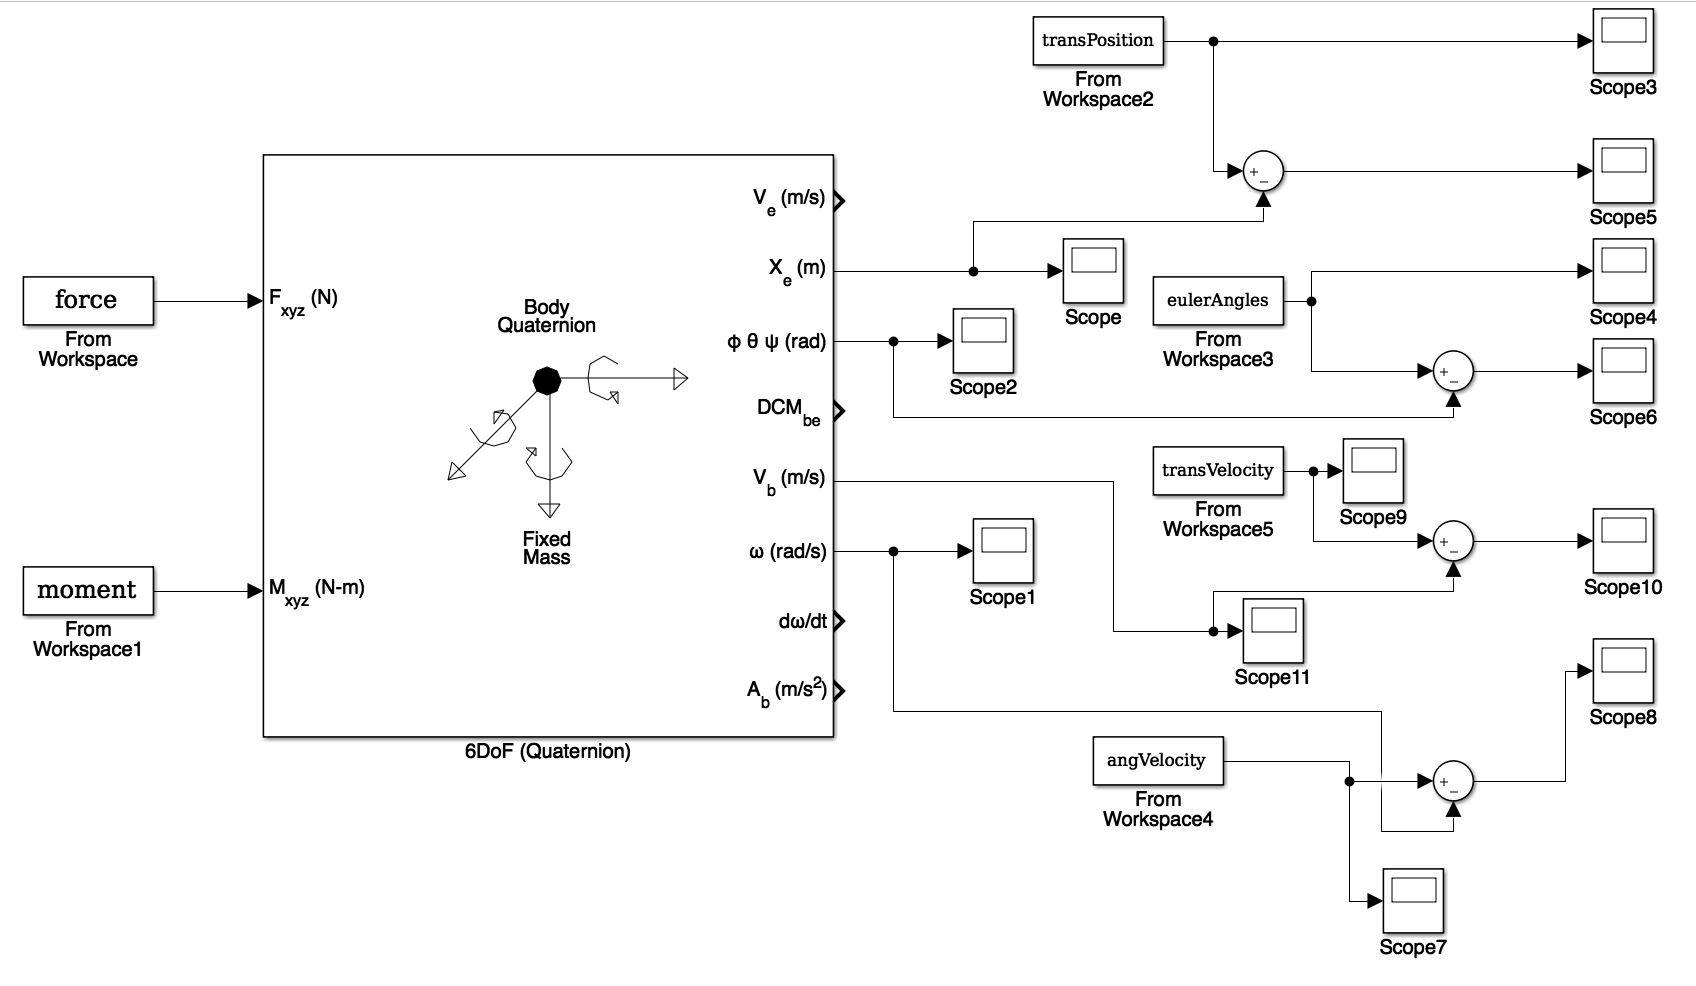
\includegraphics[width=1.1\columnwidth]{figures/validationViaSimulink}
\caption{Validation with Simulink 6DOF aircraft model. The scripted equations of motion and numeric integration are validated via Simulink's 6DOF Block. Forces and moments are directly given to the 6DOF block and the calculated states are compared with the ones calculated by the script in Matlab.}
\label{figure:validationSimulink}
\end{figure*}

\subsection{Sensor Models}

Accelerometer and gyro measurements are simulated using the angular velocity $\bm{\omega}^{B/N}_B$ and translational acceleration $\dot{\bm{v}}_B$ given by the system of equations of drone summarized in Equ.~\ref{eqn:compactEquOfMotion} and the specifications of the hardware used in \emph{Apogee Autopilot} of \emph{Paparazzi Autopilot System}.
The sensor suit simulated is the InvenSense MPU-9250 Nine-axis (Gyro + Accelerometer + Compass) MEMS MotionTracking Device.
 
The accelerometer and gyro data is simulated as 
 
 \begin{align}
\bm{z}_{gyro} &= \bm{k}_{gyro} \bm{\omega}_{B/I}^B + \bm{\beta}_{gyro} + \bm{\eta}_{gyro}\\
\bm{z}_{acc} &= \bm{k}_{acc} \bm{\omega}_{B/I}^B + \bm{\beta}_{acc} + \bm{\eta}_{acc}
% hic bir sey yazmazsan esitlikleri alt alta hizaliyor canim benim&=alo \\
% $ tek dolar arasi $ inline denklem
% $$ cift dolar arasi $$ satir atlayarak ortada denklem
\end{align}

where $\bm{\beta}$ is the bias, and $\bm{\eta}$ is the zero mean Gaussian process with $\bm{\sigma}^2$ variance with values given in Table ~\ref{arm:sensorSpecs}.

\begin{table}[!htbp]
\caption{Specifications of the sensor suit InvenSense MPU-9250 Nine-axis (Gyro + Accelerometer + Compass) MEMS MotionTracking Device\cite{condomines2015developpement}}
\label{arm:sensorSpecs}
\begin{center}
\begin{tabular}{ ||p{3cm}|p{2cm}|p{1.5cm}||}\hline
\textbf{Measurement} & $ \bm{\beta}$ &  $ \bm{\sigma}$ \\\hline
${\bm{z}_{acc}}_x$                  & $\ \ \, 0.142 $	   & $\ \ \, 0.0319$ \\\hline
${\bm{z}_{acc}}_y$       & $ -0.3 $           &  $\ \ \, 0.0985$ \\\hline
${\bm{z}_{acc}}_z$           & $\ \ \, 0.19$           & $\ \ \, 0.049$ \\\hline
${\bm{z}_{gyro}}_x$                  & $-1.55 $	   & $\ \ \, 0.0825$ \\\hline
${\bm{z}_{gyro}}_y$       & $ -1.13 $           &  $\ \ \, 0.1673$ \\\hline
${\bm{z}_{gyro}}_z$           & $-1.7$           & $\ \ \, 0.2214$ \\\hline
\end{tabular}
\end{center}
\end{table}


\subsection{Fault Models}

Probable faults in the control surfaces can be mainly grouped under two main categories \cite{zhong2014contribution}: 

\begin{itemize}
\item{A total control loss of the control surface actuators. The actuator does not respond to the control signals at all. Lock-in-place, hard-over and floating around trim are such failures (see Fig.~\ref{fig:actuatorFaults}).}
\item{A partial control loss of the control surface actuators. The actuator does respond to the control signals but does so in an abnormal way. Loss of effectiveness failure is shown in Fig.~\ref{fig:actuatorFaults}.}
\end{itemize}

When the actuators are healthy, actual control input signal will be equal to the given input signal.
In case of a fault the actual signal can be modeled as

\begin{equation}
\bm{u}\left(t\right)= \bm{E}\bm{u}_c + \bm{u}_f
\end{equation}

where $\bm{u}_c $ is the desired control signal, $\bm{E} = diag(e_1, e_2, e_3)$ is the effectiveness of the actuators where $0 \leq e_i \leq 1 $ with $(i = 1, 2 ,3)$ and $\bm{u_f}$ additive actuator fault. This model makes it possible to simulate all four types of actuator faults shown in Fig.~\ref{fig:actuatorFaults}.

%\begin{equation}
%\bm{u}\left(t\right)= \begin{bmatrix} {\delta}_{a}\ {\delta}_{e}\ n \end{bmatrix}^{\rm T}
%\end{equation}

%Here $ \delta_{a}$ aileron deflection angle in degrees, $ \delta_{e}$ elevator deflection angle in degrees, $n$ engine speed in rev/s. 


%\begin{figure}
%\begin{center}
%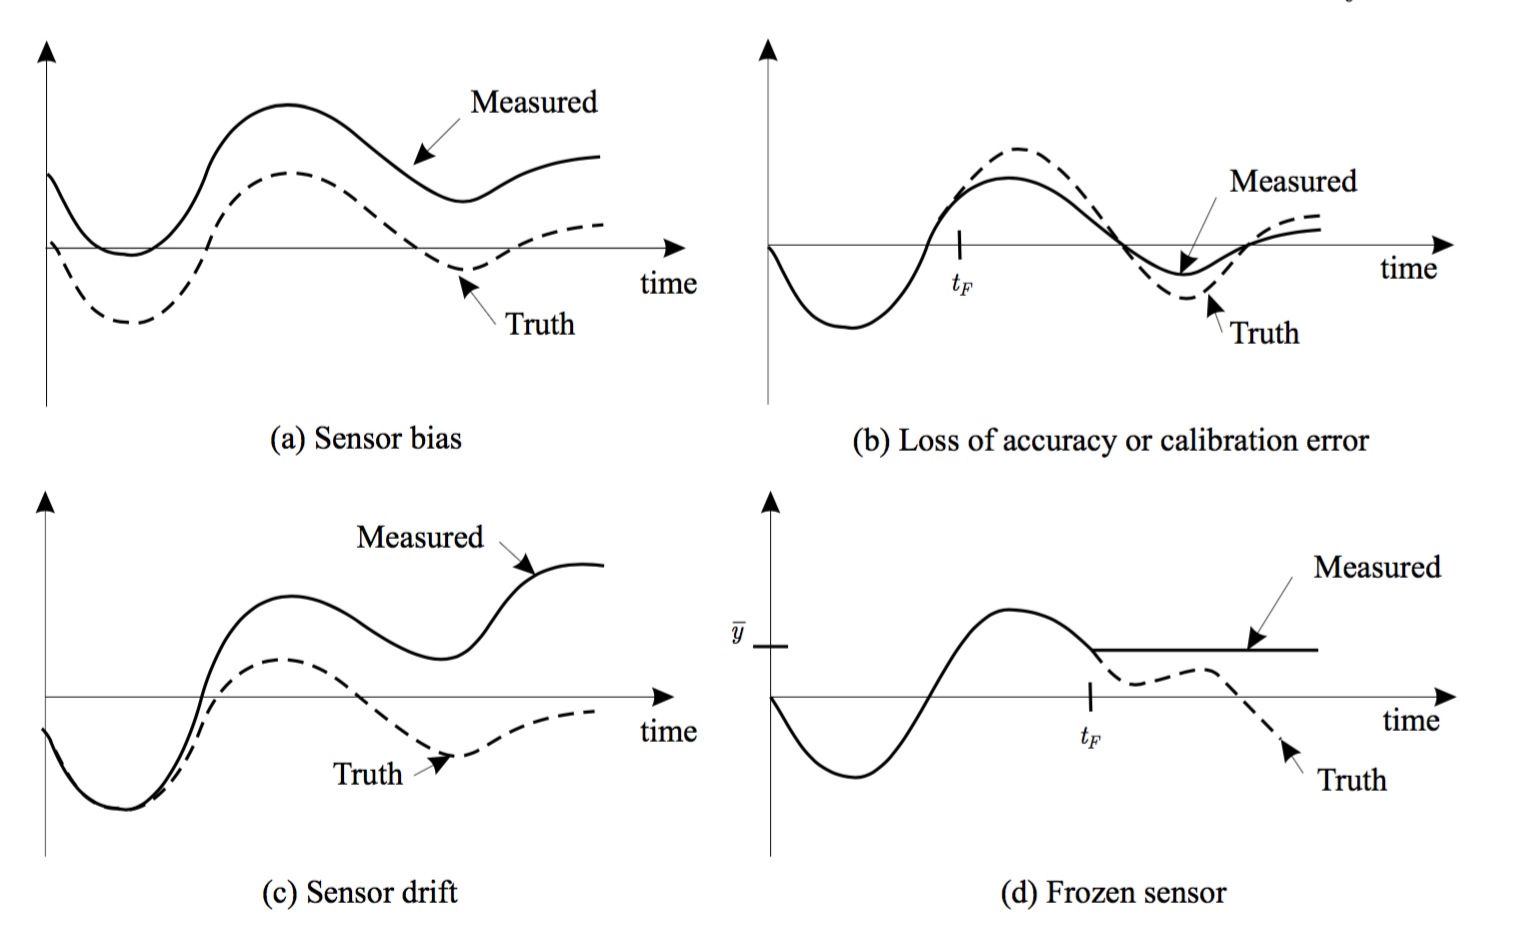
\includegraphics[width=11cm]{figures/sensorFaults}    % The printed column width is 8.4 cm.
%\caption{Probable sensor faults \cite{ducard2009fault}} 
%\label{fig:sensorFaults}
%\end{center}
%\end{figure}

\begin{figure}
\begin{center}
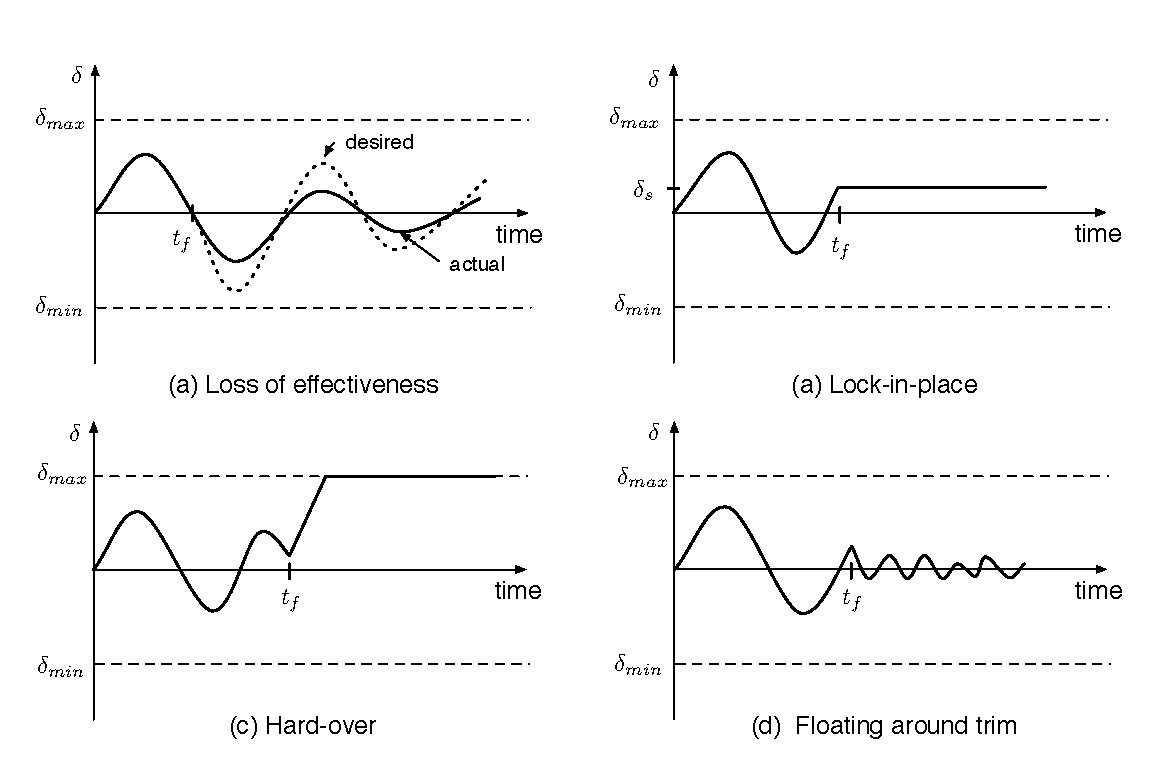
\includegraphics[width=14cm]{figures/actuatorFaults}    % The printed column width is 8.4 cm.
\caption{Probable actuator faults \cite{ducard2009fault}. (a) Loss of effectiveness: The actuator does respond to the control signals but does so in an abnormal way such as low actuation level or low response time. (b) Lock-in-place: A total control loss of the control surface actuators. The actuator freezes at a particular position. (c) Hard-over: A total control loss of the control surface actuators. The actuator freezes at the minimum or maximum position limit. (d) A total control loss of the control surface actuators. Actuator does not contribute to the control.} 
\label{fig:actuatorFaults}
\end{center}
\end{figure}




%\begin{equation}
%\bm{\dot{x}}\left(t\right) = \bm{f}\left(\bm{x}\left(t\right) , \bm{u}\left(t\right) \right) 
%\end{equation}


%\begin{align}
%{{\mu }_{nf}}\frac{{{\partial }^{2}}u}{\partial {{y}^{2}}}+{{\left( \rho \beta  \right)}_{nf}}g\sin \phi \left( T-{{T}_{w2}} \right)-{{\sigma }_{nf}}B_{0}^{2} \sin^{2}\left( \alpha + \phi \right) u&=\frac{\partial p}{\partial x}  \label{equ1} \\
%\frac{{{\partial }^{2}}T}{\partial {{y}^{2}}}+\frac{{{\mu }_{nf}}}{{{k}_{nf}}}{{\left( \frac{\partial u}{\partial y} \right)}^{2}}+\frac{{{\sigma }_{nf}}}{{{k}_{nf}}}B_{0}^{2} \sin^{2}\left( \alpha + \phi \right){{u}^{2}}&=0 \label{equ2} \ 
% hic bir sey yazmazsan esitlikleri alt alta hizaliyor canim benim&=alo \\
% $ tek dolar arasi $ inline denklem
% $$ cift dolar arasi $$ satir atlayarak ortada denklem
%\end{align}
%%%%% End of Eq 1 & Eq 2 %%%%%
%The system of equations in  Eq (1-2) is subject to boundary conditions given in (3-4)
%%%%%% Eq 3 & Eq 4 %%%%%%
%\begin{align}
%u(H / 2)&=0   & u(-H / 2)&=0\\
%T(H / 2)&= {T}_{w1} & T(- H / 2)&= {T}_{w2}0
%\end{align}

%\begin{figure}
%\begin{center}
%\includegraphics[width=8.3cm]{FTCmethods}    % The printed column width is 8.4 cm.
%\caption{Variations of fault tolerant control systems } 
%\label{fig:FTCmethods}
%\end{center}
%\end{figure}

%\begin{table}
%\caption{Attitude representations comparison}
%\label{tab:attRepSelection}
%\begin{center}
%\begin{tabular}{||l|l||}\hline
%Representation & Number of parameter set & Properties \\\hline
%our	   & friends \\\hline
%\end{tabular}
%\end{center}
%\end{table}

\section{Conclusion}
In this chapter, equations of motion of an aircraft are given. 
Motion of an aircraft usually involves both translation and rotation. 
Here, equations for translational and rotational motion are discussed separately in detail.
After the equations are derived for a generic aircraft, calculation of forces and moments which are specific to an individual drone is presented (Aerodynamic force derivatives and stability derivatives are specific for each drone). For two different drone examples, a drone from ETH Zurich and MAKO (used in ENAC UAV LAB), calculation of forces and moments are given.
Those forces and moments are inputs to the dynamic equations of motion. 

The models derived here are not used in detection and diagnosis algorithms. 
The detection and diagnosis algorithms used in this thesis use only data. 
The need for data is the driving factor to simulate the drone motion. 
Thus, data is simulated using MAKO drone model and specifications of IMU \emph{InvenSense MPU-9250 Nine-axis} used in \emph{Paparazzi Autopilot Apogee} onboard. 
 
%To clarify, machine learning methods also train a model. 
%But in that case, the model is not the equations of motion of an aircraft but rather a simpler model and may not explicitly describe the physical . 
%The only exception to not using physical models in this work for diagnosis, is the part that the diagnosis is realized using spinors as features. To calculate the spinors, kinematic equations are numerically. But still, our idea to generalize by having no models holds since only kinematic equations are used. 

In this thesis, the diagnosis is implemented on two types of data: 1. Simulated data, 2.
Flight data. 
If the reader is not interested in detection and diagnosis via simulated data, s/he can skip this chapter since this chapter explains the models that are used to simulate measurements.
Even then, having a background information on the physics of the system might help to have a grasp on the features (translational acceleration and angular velocities) used in both model-based and data-driven fault diagnosis.

Since the data is generated and available now for implementations, the methodology used in this thesis to diagnose faults are discussed in the next chapter. 
In this thesis, \emph{Support Vector Machines} (SVM) are used as a classification method to diagnose faults onboard a drone. 
Since SVM is a machine learning method, an introduction to machine learning methods have been given from an implementation perspective. 
It starts with an introduction to terminology for machine learning methods, gives general explanations to prepare the inputs to the machine learning algorithm. 
Then many application details are discussed that would help to user to apply those methods to their own problems. 
Finally, SVM is introduced and three phases encountered during its implementation, \emph{training}, \emph{tuning} and \emph{evaluation} is explained.



%% This is an example first chapter.  You should put chapter/appendix that you
%% write into a separate file, and add a line \include{yourfilename} to
%% main.tex, where `yourfilename.tex' is the name of the chapter/appendix file.
%% You can process specific files by typing their names in at the 
%% \files=
%% prompt when you run the file main.tex through LaTeX.
\chapter{Methodology}

In this chapter, an introduction to machine learning methods is presented. 
Machine learning methods have been discusses with a focus on applications rather then the theory.
Finally, a supervised learning method, Support Vector Machines (SVM) is explained since it is the method used for classification in this thesis.

\section{Machine Learning}

The aim of machine learning methods is to train a model with a given data set in order to predict the output values corresponding to a new input. 
According to Arthur Samuel, name father of machine learning, "Machine learning is the field of study that gives computers the ability to learn without being explicitly programmed". 
A rather more to the point but complicated definition offered by Tom Mitchell in 1998, quite new compared to Samuel\textquotesingle s in 1959, "A computer program is said to learn from experience E with respect to some task T and some performance measure P, if its performance on T, as measured by P, improves with experience E".

\subsection{Introduction}
Machine learning methods are mainly handled under two main categories: supervised and unsupervised learning as shown in Fig.~\ref{fig:machineLearningMethods}. 

\begin{figure}
\begin{center}
\includegraphics[width=14cm]{figures/machineLearningMethods}    % The printed column width is 8.4 cm.
\caption{Common machine learning methodologies} 
\label{fig:machineLearningMethods}
\end{center}
\end{figure}

In supervised learning, \textit{"right answers"} are available for each training input in the data set.
Supervised learning methods are comprised of two phases, the learning and the prediction as shown in Fig.~\ref{fig:supervisedLearningBasics}.
The first phase is comprised of learning from the available data to understand how the system behaves. 
In the second phase, the idea is to predict what will be the output of the system for a given input, depending on the knowledge about the system that you gained via learning phase. 

\begin{figure}
\begin{center}
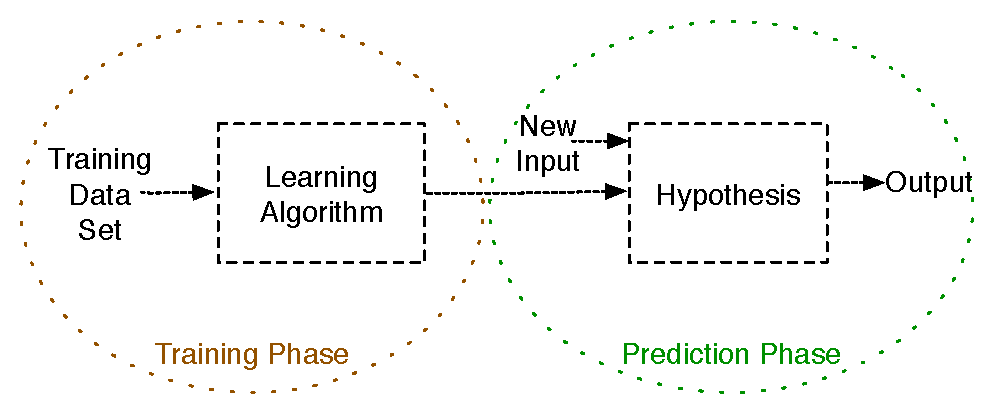
\includegraphics[width=14cm]{figures/supervisedLearningBasics}    % The printed column width is 8.4 cm.
% For the old picture 
% \includegraphics[width=12cm]{figures/machineLearningBasics}   
\caption{Supervised learning basics } 
\label{fig:supervisedLearningBasics}
\end{center}
\end{figure}
 
The most common types of supervised leaning is the regression and classification problems. 
Since these are both of supervised learning types, the \textit{"right answer"} (right values of the output $y$) for each example is assumed to be known. 

In unsupervised learning, the \textit{"right answers"} corresponding to the training input are not available. 
There are other machine learning algorithms, such as reinforcement learning, that is a combination of supervised and unsupervised learning. 

\subsection{Terminology}

A basic introduction to frequently used terms in machine learning is given in this section.  
Table~\ref{arm:machineLearningTerminology} shows representations of commonly used variables in machine learning. 
Although representations could differ from one reference to the other, throughout this thesis, one coherent representation given in Table~\ref{arm:machineLearningTerminology} is followed. 

\begin{table}
\caption{Machine learning terminology}
\label{arm:machineLearningTerminology}
\begin{center}
\begin{tabular}{||l|l||}\hline
x & input variable or feature \\\hline
y & output variable or target variable \\\hline
\textbf{X} & input variable vector or feature vector \\\hline
\textbf{y} & output variable vector or target variable vector \\\hline
m & number of training examples \\\hline
n & number of features \\\hline
i & index of training examples \\\hline
j & index of features \\\hline
$\textbf{x}_j^{(i)}$ & $i^{th}$ training example for feature $j$ \\\hline
$\textbf{y}^{(i)}$ & $i^{th}$ training output  \\\hline
$\textbf{h}_{\bm{\theta}}(\textbf{x})$ &hypothesis function (model)\\\hline
$\bm{\theta}$ &parameter set\\\hline
$\textbf{J}({\bm{\theta}})$ &cost function  \\\hline

\end{tabular}
\end{center}
\end{table}

Many of the machine learning tools, such as \emph{MATLAB Statistics and Machine Learning Toolbox} or \emph{Tensorflow}, have defaults settings and are easy to be used by beginners. 
Although they would most probably not achieve optimized results which would be the case in the hands of an experienced user, a beginner can easily start using those tools by sending input and output vectors as arguments to the machine learning functions. 

The configurations of input and output vectors to feed the learning algorithms might change from one to other but still there is a common convention that would be compatible with many. 
In this representation, each instance is given in different rows of the input vector. 
An example of predicting housing prices taken from Ref.~\cite{andrewNgMachLearning} is given to show the way to constitute the input and output matrix. 
Table~\ref{arm:exampHousingPrices} uses a supervised learning regression example to show input and output vector representations. 
The aim of the problem in this example is to predict price of houses for given surface area. 
For that, known examples of houses with surface area and corresponding price have been given. 
Since the aim of the problem is to predict the price of a house given the surface area, price of house is the output of the problem. 
And to predict the price, the available information that is known to effect the price of a house is the surface area of the house, making it the input variable. 
So, in Table~\ref{arm:exampHousingPrices} each row corresponds to a different house, second column (surface area of house) constitute the input vector and the last row (price in 1000s) corresponds to the output vector. 

\begin{table}
\caption{Training set $(\textbf{x},\textbf{y})$ of housing prices - one-feature example}
\label{arm:exampHousingPrices}
\begin{center}
\begin{tabular}{ || c | c | c ||}\hline
\textbf{training example index} $(i)$ & \textbf{Size in $feet^2$} ($\textbf{x}$) & \textbf{Price in $1000 \$ s$} ($\textbf{y}$) \\\hline
1 & 2104	   & 460 \\\hline
2 & 1416	   & 232 \\\hline
3 & 1534	   & 315 \\\hline
4 & 852	   & 178 \\\hline
$\vdots$ & $x^{(i)}$   & $y^{(i)}$ \\\hline
m & $x^{(m)}$   & $y^{(m)}$ \\\hline
\end{tabular}
\end{center}
\end{table}

In this problem, there is an assumption that the price of a house is only dependent on the surface area which would not hold in the real case. 
In real problems, it is more common that the output would depend not only one variable but more, or many. 
For that reason, the input vector in a realistic example would rather be an input matrix having different features in its columns as given in Table~\ref{arm:exampleMultiFeatures}. 
Here in this example, the output is still the price of house, but now the features which corresponds to each column of an input matrix (or sometimes called the feature matrix) are surface area, number of bedrooms, and can be enlarged until n features. 
It should be kept in mind that the selection of features that would lead to a better prediction of the output is a challenging problem and usually requires experience on the system of interest. 

\begin{table}
\caption{Training set $(\textbf{x},\textbf{y})$ of housing prices - multi-feature example}
\label{arm:exampleMultiFeatures}
\begin{center}
\begin{tabular}{ ||p{2cm}|p{2cm}|p{2cm}|p{2cm}|p{2cm}|p{2cm}||}\hline
\textbf{training example index} $(i)$ & \textbf{Size in $feet^2$} ($\textbf{x}_1^{(i)}$) & \textbf{Number of bedrooms} ($\textbf{x}_2^{(i)}$) & \textbf{Feature j} ($\textbf{x}_j^{(i)}$) & \textbf{Feature n} ($\textbf{x}_n^{(i)}$) &\textbf{Price in $1000 \$ s$} ($\textbf{y}$) \\\hline
1 & 2104	& 5  & $\textbf{x}_j^{(1)}$ & $\textbf{x}_n^{(1)}$ & 460 \\\hline
2 & 1416 & 3 & $\textbf{x}_j^{(2)}$ & $\textbf{x}_n^{(2)}$ & 232 \\\hline
3 & 1534 & 3 & $\textbf{x}_j^{(3)}$ & $\textbf{x}_n^{(3)}$ & 315 \\\hline
4 & 852 & 2 & $\textbf{x}_j^{(4)}$ & $\textbf{x}_n^{(4)}$ & 178 \\\hline
$\vdots$ & $\textbf{x}_1^{(i)}$  & $\textbf{x}_2^{(i)}$  & $\textbf{x}_j^{(i)}$   & $\textbf{x}_n^{(i)}$ & $\textbf{y}^{(i)}$ \\\hline
m & $\textbf{x}_1^{(m)}$  & $\textbf{x}_2^{(m)}$  & $\textbf{x}_2j^{(m)}$   & $\textbf{x}_n^{(m)}$ & $\textbf{y}^{(m)}$ \\\hline
\end{tabular}
\end{center}
\end{table}


%\clearpage
%\newpage


\subsection{Steps towards the learning machine}

\subsubsection{Visualizing the data}

Having a preliminary glance at data might give the designer an idea about the ways to tackle the problem since it is the designer to select the features, the model, and the type of cost function. 
It is true that the algorithms are optimizing some parameters of the model and the cost function but still the structure itself is usually supplied by a human. 
Although there are tricks to select those in a better sense, machines still have a way to go towards Skynet\footnote{From movie Terminator: ``Skynet is a fictional neural net-based conscious group mind and artificial general intelligence (see also superintelligence) system that features centrally in the Terminator franchise and serves as the franchise's true main antagonist.''}.

Fig.~\ref{fig:housingPrices} shows the housing price depending on the surface area corresponding to the data given in Table~\ref{arm:exampHousingPrices}.
In this example, price of the houses are the output (target) variable given in y-axis and size (surface area in $feet^2$) is the feature (input) variable given in x-axis. 
Since output y is price which is a continuous value (thus not a label representing a class) this problem is called a regression problem. Plotting the data given shows that the problem could to be modeled by a linear model (a linear line to fit the data given). Then linear regression can be applied.

\begin{figure}
\begin{center}
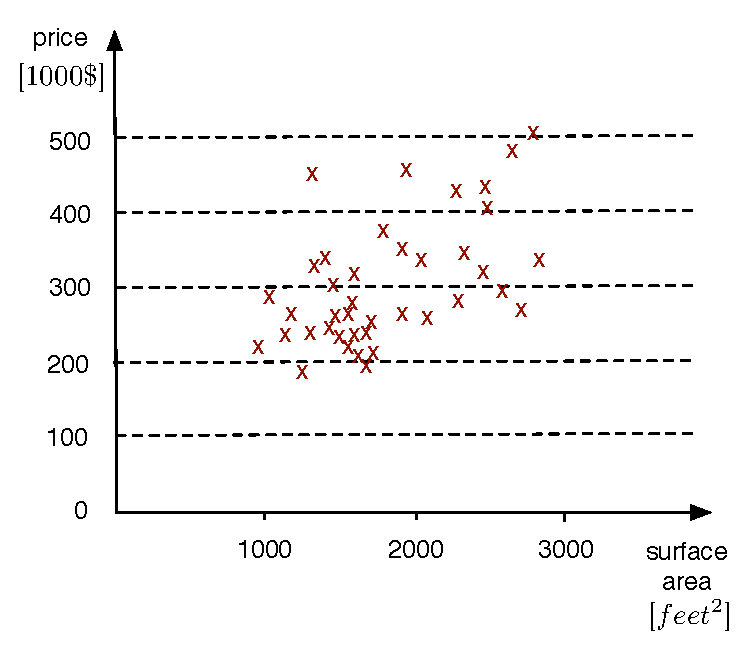
\includegraphics[width=11cm]{figures/linearRegressionExamp}    % The printed column width is 8.4 cm.
\caption{Regression example - Housing prices as a function of surface area of the house \cite{andrewNg_MachLearning}} 
\label{fig:housingPrices}
\end{center}
\end{figure}

\begin{figure}
\begin{center}
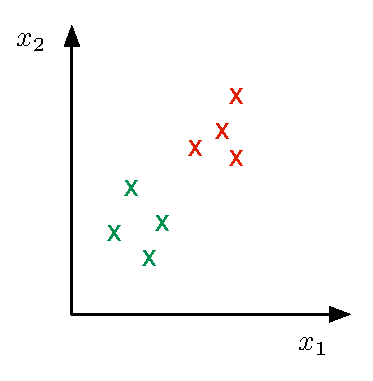
\includegraphics[width=5cm]{figures/classificationEx2}    % The printed column width is 8.4 cm.
\caption{Classification example} 
\label{fig:classificationEx2}
\end{center}
\end{figure}

Since an example for regression problem has been given, now a preliminary look at classification problem will be presented. 
Fig.~\ref{fig:classificationEx2} is a classification problem since the aim is to distinguish the class that a new input instance will belong to. 
Here the vertical dimension is not the output as in the previous example of linear regression but is another feature ($x_2$ in this example). 

And the information about the output is represented with the colors of the samples in the feature space.
Fig.~\ref{fig:classificationEx1} shows the output vs. inputs of a classification problem. 
This is just to show the difference between regression and classification problem figures. 
Usually in regression problems the y-axis represents the output. 
Here, there is a direct analogy by representing a classification problem just as a regression problem, x-axis representing the input whereas y-axis representing the output. 
But usually in classification problems, value of y (which class it corresponds to) is represented with different colors as in Fig.~\ref{fig:classificationEx2} or with different signs such as O and X.

By just plotting the samples, in this example, it seems that logistic regression could yield satisfactory results since the data seems to be separated by a linear decision boundary. 
A decision boundary is a curve which separates the training data examples which belongs to different classes. 

It is possible to choose the model structure that would represent the problem satisfactorily via visualizing the data set when the number of features are not large.
With an increasing number of feature set, determining the degree of the polynomial via visualizing the data to represent the input output relationship could be more complicated. 
In that case, the user should refer to model selection techniques rather than the insights gained by data visualization. 


\begin{figure}
\begin{center}
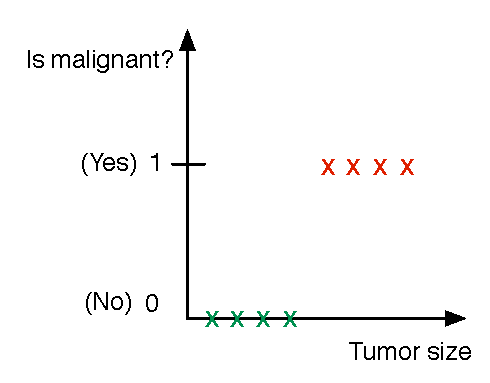
\includegraphics[width=7cm]{figures/classificationEx1}    % The printed column width is 8.4 cm.
\caption{Classification example - output vs input} 
\label{fig:classificationEx1}
\end{center}
\end{figure}

In case the number of feature set is small but yet the visualization gives that the model for regression or classification problem can not be represented by a linear model (or linear decision boundary), feature mapping could be applied. 
Then linear regression or logistic regression (can only fit linear models unless features are mapped) could be applied to nonlinear systems with mapped features.  

\subsubsection{Feature Mapping}

This section applies to problems with smaller feature sets and to fit a nonlinear model with linear or logistic regression.
Depending on the results from visualizing data, it might be necessary to map the features since a straightforward implementation of linear / logistic regression might result in linear model, linear decision boundary respectively. 
So for the cases that a linear model will not be satisfactory enough to describe the training data, feature mapping should be applied.

The housing price prediction problem can be revisited here to give an example on feature mapping.
The data given in Table~\ref{arm:exampHousingPrices} and plotted in Fig.~\ref{fig:housingPrices} is a regression problem with one feature (surface area of house).
To fit more accurately to the training data given, new features can be artificially added to the system as below, where the new features will be functions of the original feature.

\begin{align}
\label{eqn:costFuncExamp1}
\begin{split}
h_{\theta}(\bm{x}) & = \theta_0 + \theta_1 x_1 + \theta_2 x_2 + \theta_3 x_3
\\
& = \theta_0 + \theta_1 (size) + \theta_2 {(size)}^2 + \theta_3 {(size)}^3
\end{split}
\end{align}

where

\begin{align}
\label{eqn:featureMapping1}
\begin{split}
x_1 & = size
\\
x_2 & = size^2
\\
x_3 & = size^3
\end{split}
\end{align}

\begin{figure}
\begin{center}
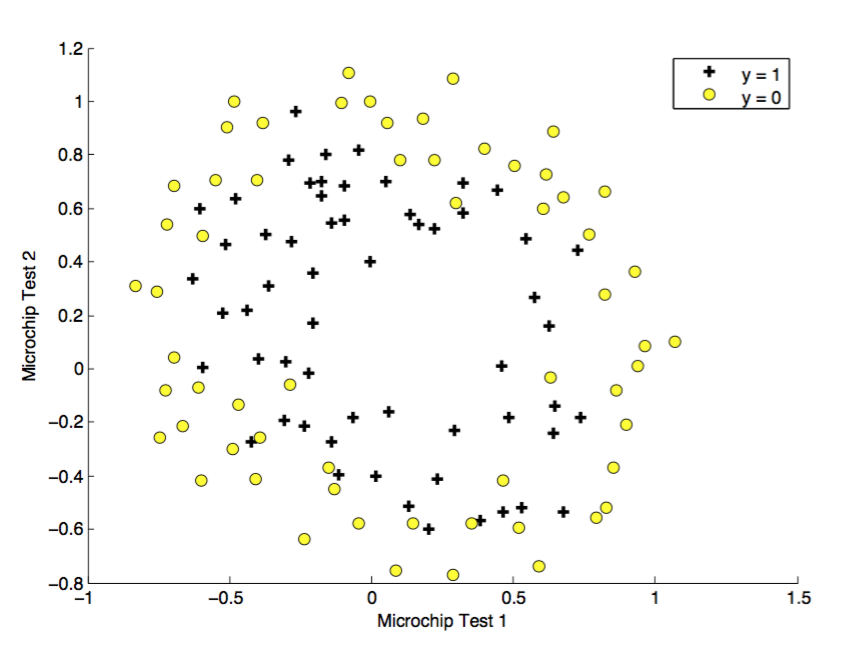
\includegraphics[width=13cm]{figures/classificationMicrochip}    % The printed column width is 8.4 cm.
\caption{Classification example - complex decision boundaries \cite{andrewNg_MachLearning}} 
\label{fig:classificationEx3}
\end{center}
\end{figure}

By changing the model via adding features, now it is possible to fit a nonlinear curve to the training data as given in Fig.~\ref{fig:underOverFit}.

Another example that requires a nonlinear model to fit the data set is microchip assessment problem.
This example is also taken from the lecture notes of machine learning course by Andrew Ng \cite{andrewNgMachLearning}. 
This is a two class classification problem, where one class of microchips is faulty while the other class is functional.
It is seen from the Fig.~\ref{fig:classificationEx3} that a linear decision boundary will not serve appropriately to classify the data. 
So, in order to apply logistic regression for this problem, feature mapping is necessary. 
An example of a mapped feature vector that could give a satisfactory decision boundary to classify the two classes could be given as

\begin{equation}{\label{eqn:featureMapping2}}
\bm{x_{mapped}}
=\,
\begin{bmatrix}
1 & x_1 & x_2 & x_1^2 & x_1x_2 & x_2^2 & x_1^3 \cdots & x_1x_2^5 & x_2^6 
\end{bmatrix}
\,^ T
\end{equation} 

Mapping of the features could be done in various ways. 
Let's take another example of binary (two-class) classification problem with 100 features, which needs a nonlinear decision boundary to achieve a satisfactory classification.
One way to map the feature set could be such that only the quadratic terms are taken into account, which would result in a new feature set such as
 
\begin{equation}{\label{eqn:featureMapping3}}
\bm{x_{mapped}}
=\,
\begin{bmatrix}
x_1^2 & x_1x_2 & x_1x_3 & \cdots & x_1x_{100} & x_2^2 & x_2x_3 & \cdots & x_3^2 & x_3x_4  \cdots  
\end{bmatrix}
\,^ T
\end{equation} 

with a complexity $O(n^2) \sim \frac{n^2}{2}$

If 3rd order terms are considered, the new feature set becomes

\begin{equation}{\label{eqn:featureMapping4}}
\bm{x_{mapped}}
=\,
\begin{bmatrix}
x_1^3 & x_1x_2x_3 & x_1^2x_2 & \cdots  & x_{11}x_{13}x_{17} & \cdots  
\end{bmatrix}
\,^ T
\end{equation} 

\begin{figure}
\begin{center}
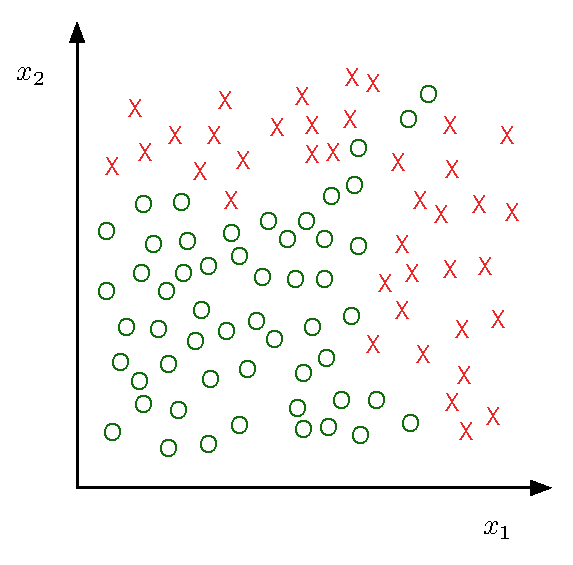
\includegraphics[width=6cm]{figures/complexDecisionBoundary}    % The printed column width is 8.4 cm.
\caption{Classification example - complex decision boundaries} 
\label{fig:complexBoundary}
\end{center}
\end{figure}

\begin{figure}
\begin{center}
\includegraphics[width=14.1cm]{figures/ml_followChart}    % The printed column width is 8.4 cm.
\caption{Simplified guide for feature mapping} 
\label{fig:ml_followChart}
\end{center}
\end{figure}


It is important to point out that, with a higher dimensional feature vector, the model will tend to fit more accurately to the training set but might be poor to generalize for a new input. 
This is called overfitting which is a common problem for many machine learning applications. 
More explanations about overfitting and ways to overcome it will be explained in regularization section. 
Increasing the dimensionality of the features, the model might become more computationally expensive as well.

To fit a model or decision boundary of a circular or elliptical shape, only a subset of features can be considered such as

\begin{equation}{\label{eqn:featureMappin54}}
\bm{x_{mapped}}
=\,
\begin{bmatrix}
x_1^2 & x_2^2 & x_3^2 & \cdots & x_N^2  
\end{bmatrix}
\,^ T
\end{equation} 

Finally, when the number of features are small, but it can not fit complex models or boundaries such as in Fig.~\ref{fig:complexBoundary}, then addition of higher terms such as given in 
Equ.~\ref{eqn:featureMapping3} or using Neural Networks should be considered.
A scheme to help select the strategy for mapping is given in  Fig.~\ref{fig:ml_followChart}. 

\subsubsection{Vectorized form of the problem}

The model can be written in a vectorized form to accommodate larger feature sets in a more compact form.
To write in the compact form, and an extra feature $\bm{x}_0 = 1$ is added to the feature vector such as

\begin{equation}{\label{eqn:featureVector}}
\bm{x}
=\,
\begin{bmatrix}
x_0 \quad x_1 \quad x_2 \quad \cdots \quad x_n 
\end{bmatrix}
^T
\end{equation} 

 Fig.~\ref{fig:addArtificialFeature} shows the addition of the artificial feature in the feature matrix.

\begin{figure}
\begin{center}
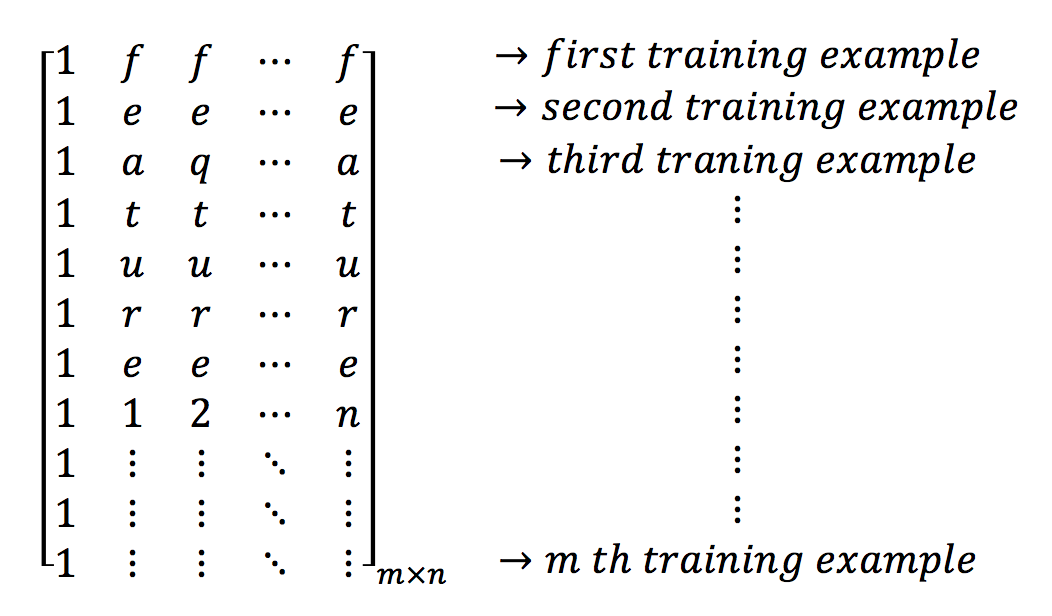
\includegraphics[width=9cm]{figures/addArtificialFeature}    % The printed column width is 8.4 cm.
\caption{Adding an artificial feature of 1s.} 
\label{fig:addArtificialFeature}
\end{center}
\end{figure}

Also parameters of the model is given in vectorial form such as

\begin{equation}{\label{eqn:parameterVector}}
\bm{\theta}
=\,
\begin{bmatrix}
\theta_0\quad \theta_1 \quad  \theta_2 \quad \cdots \quad \theta_n 
\end{bmatrix}
^T
\end{equation} 

So for the linear regression problem with a single feature, the model is given as

\begin{equation}{\label{eqn:costFuncOneFeature}}
h_{{\bm{\theta}}}(x) = \theta_0 + \theta_1 x_1
\end{equation} 

and the model for $n$ features

\begin{equation}{\label{eqn:costFuncMltplFeature}}
h_{{\bm{\theta}}}(x) = \theta_0 + \theta_1 x_1 + \theta_2 x_2 + \cdots+ \theta_n x_n
\end{equation}

Introducing the vectorial forms of $\bm{x}$ and $\bm{\theta}$ enables the model to be written in compact generic form such as 

\begin{equation}{\label{eqn:costFuncMltplFeature}}
h_{{\bm{\theta}}}(x) = {\bm{\theta}}^\intercal \bm{x}
\end{equation}

\subsubsection{Cost Function}

To calculate $\bm{\theta}$ that will fit a better model to the training data, optimization algorithms are used to minimize the cost function $J({\bm{\theta}})$.
Usually, cost function and its gradient are given to the optimization algorithm as an input. 
Here, widely used cost functions for linear regression (regression problem) and logistic regression (classification problem) are given. 

Cost function for linear regression can be given as

\begin{equation}{\label{eqn:costFuncLinearRegression}}
J({\bm{\theta}})
=\,
\frac{1}{2m} \sum\limits_{i=1}^{m} \Big(h_{\bm{\theta}}(x^{(i)}) - (y^{(i)})\Big)^2  
\end{equation} 

and the cost function for logistic regression (classification) is given for two class classification problem (e.g $y \in \{0,1\}$) as 

\begin{equation}{\label{eqn:costFuncLogisticRegression}}
J({\bm{\theta}})
=\,
\frac{1}{m} \sum\limits_{i=1}^{m} \Big[-y^{(i)}log(h_{\bm{\theta}}(x^{(i)})) - (1-(y^{(i)}))log(1-h_{\bm{\theta}}(x^{(i)}))\Big]
\end{equation} 


\subsubsection{Selecting the model}

With a larger set of features, it might be difficult to have a sense of which model would be a better fit to the problem via visualizing the data. 
In this cases, model selection techniques could be applied to decide which model will yield to a better accuracy.

To explain the procedure, first assume a model structure is already selected or given. 
In such a problem, during training, training data is used to calculate the best model parameter vector $\bm{\theta}$ that would minimize the objective function, $J_{tranining}(\bm{\theta)}$.
Then trained model is assesses with a new data set $J_{test}$, since the evaluation would be biased in favor of the training data that the model is trained for. 
That could lead to an optimistic view of the abilities of the learning algorithm. 

In model selection technique, each model is given a number $d$ to represent the model as shown below.

\begin{alignat*}{6}
\label{eqn:exampCostFunc}
d &= 1, \quad h_{{\bm{\theta}}}(x) \ && = \theta_0 + \theta_1 x\ \ && \longrightarrow \theta^{(1)}\ \ && \quad \longrightarrow J_{cv}(\theta^{(1)})\
\\
d &= 2, \quad h_{{\bm{\theta}}}(x) \ && = \theta_0 + \theta_1 x + \theta_2 x^2 \ \ && \longrightarrow \theta^{(2)}\ \ && \quad \longrightarrow J_{cv}(\theta^{(2)})\
\\
d &= 3, \quad h_{{\bm{\theta}}}(x) \ && = \theta_0 + \theta_1 x + \theta_2 x^2 + \theta_3 x^3\ \ && \longrightarrow \theta^{(3)}\ \ && \quad \longrightarrow J_{cv}(\theta^{(3)})\
\\
& \ &&\ \vdots \ &&\ \ &&\ 
\\
d &= k, \quad h_{{\bm{\theta}}}(x) \ && = \theta_0 + \theta_1 x_1 + \cdots+ \theta_k x^k\ \ && \longrightarrow \theta^{(k)}\ \ && \quad \longrightarrow J_{cv}(\theta^{(k)})\
\end{alignat*}

In the previous problem of a given model structure, only model parameter vector $\bm{\theta}$ is calculated to minimize cost function $J_{training}(\bm{\theta)}$.
Now, since the best model is not known, it is also necessary to find the best $d$ to minimize the cost function. 
Since now the parameters to fit for is two, $\bm{\theta}$ and $d$, three different sets of data is necessary to evaluate, in order to avoid overfitting.
As for the case of training and evaluating with the same data in the previous paragraph for a given model, using only two data sets and calculating the test set error with the same data that is used for selecting the model, might lead to selecting a model biased towards the data that is used selecting the model.
 
So, the idea is to have different subsets of data to train the model (calculating ${\bm{\theta}}$), to select the model structure and to evaluate the selected model structure and its corresponding parameter set. 
In order to do that, 3 distinct data sets are needed as shown in Fig.~\ref{fig:modelSelection}, to train parameters ${\bm{\theta}}$, to select the model structure $d$, and associate an error value to the chosen model. 
Then, the model structure coined by number $d$ which makes $J_{cv}({\bm{\theta}}^{(d)})$ minimum is selected and its generalization is error is calculated with the test set $J_{test}({\bm{\theta}}^{(d)})$.

Fig.~\ref{fig:modelSelection} summarizes the steps to be followed which are explained in more detail as

\begin{enumerate}
  \item Train the model for each model structure (d = 1,2,3 .. k) by using the training set (60\% of whole data, randomly selected) which will output the parameters ${\bm{\theta}}^{(d)}$ for the corresponding model $(d)$.
  This phase is explained with more details in section \emph{Calculating parameters ${\bm{\theta}}$}. But the general idea is to calculate the ${\bm{\theta}}$ that will minimize the cost function $J_{training}$ given as

\begin{equation}{\label{eqn:costFuncTraining}}
J_{training}({\bm{\theta}})
=\,
\frac{1}{2m_{training}} \sum\limits_{i=1}^{m_{training}} \Big(h_{\bm{\theta}}(x_{training}^{(i)}) - (y_{training}^{(i)})\Big)^2  
\end{equation}   
  
  \item Then by using the cross validation data set (20\% of whole data, randomly selected) calculate cross validation error for each model and select the model with the smallest cross validation error.

\begin{equation}{\label{eqn:costFuncCrossVal}}
J_{cv}({\bm{\theta}})
=\,
\frac{1}{2m_{cv}} \sum\limits_{i=1}^{m_{cv}} \Big(h_{\bm{\theta}}(x_{cv}^{(i)}) - (y_{cv}^{(i)})\Big)^2  
\end{equation} 

  \item Then by using the test set (20\% of whole data, randomly selected) estimate generalization error for the selected model.
  
\begin{equation}{\label{eqn:costFuncTest}}
J_{test}({\bm{\theta}})
=\,
\frac{1}{2m_{test}} \sum\limits_{i=1}^{m_{test}} \Big(h_{\bm{\theta}}(x_{test}^{(i)}) - (y_{test}^{(i)})\Big)^2  
\end{equation} 

\end{enumerate}

\subsubsection{Normalization (Scaling)}

The next step is to normalize the data in order to constrain the values of features change within the same order of magnitude. 
This helps to improve the convergence rate of the optimization algorithm during the calculation of the model parameters $\bm{\theta}$.  
Although there are different methods for normalization, a common way is

\begin{equation}{\label{eqn:scalingFeatures}}
\bar{x}_j = \frac{x_j - \mu_j}{s_j} 
\end{equation} 

where the mean $\mu_j$ and range $s_j$ is given as

\begin{landscape}
\begin{figure}
\begin{center}
%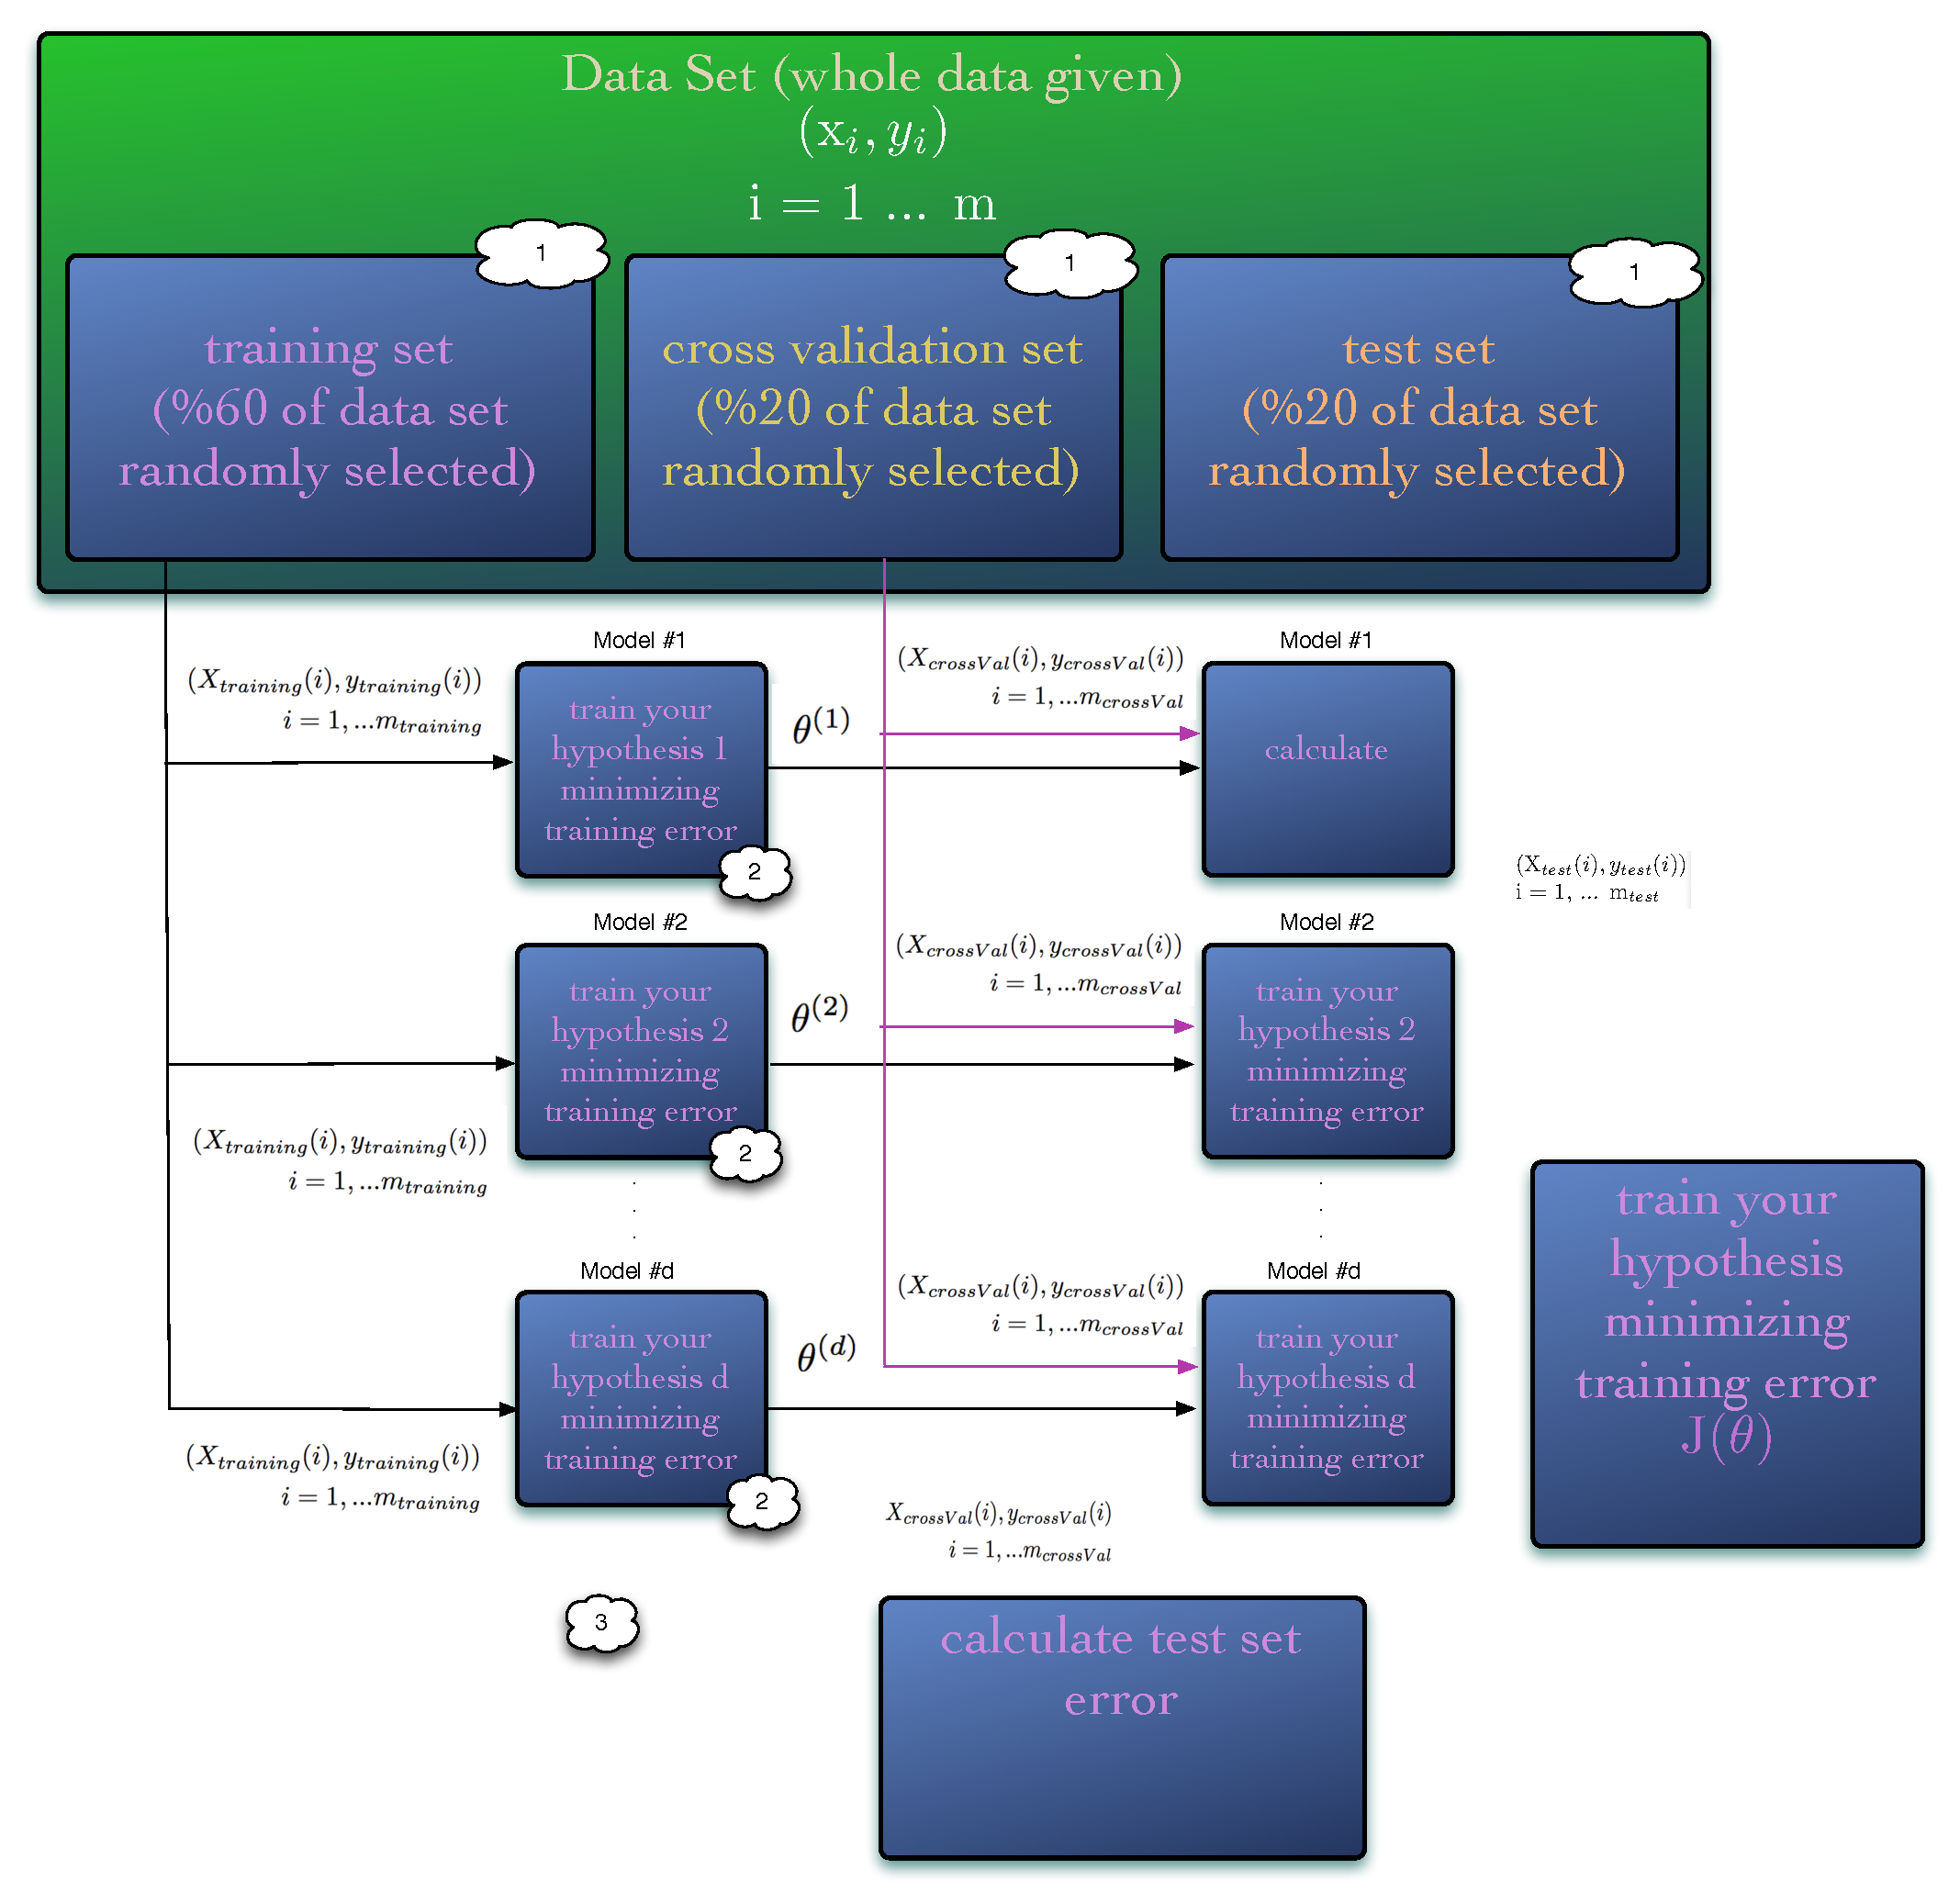
\includegraphics[width=16cm]{figures/modelSelection}    % The printed column width is 8.4 cm.
\includegraphics[width=23cm]{figures/modelSelectionNonVisualizableData}    % The printed column width is 8.4 cm.
\caption{model selection guide} 
\label{fig:modelSelection}
\end{center}
\end{figure}
\end{landscape}



\begin{align}
\label{eqn:meandAndRange}
\begin{split}
\mu_j & = \frac{\sum\limits_{i=1}^m {x_j^i} }{m}
\\
s_j & = max(x_j) - min(x_j)
\end{split}
\end{align}

An important point is to keep that values $\mu_j$ and $s_j$ (or standard deviation in cases it is preferred instead of range $s_j$). 
Those values are saved since they will also be used to scale the new inputs during the prediction phase.


\subsubsection{Training and Evaluating of the classifier}

Here, it is assumed that we have selected one model and train the parameters of only this model selected. 
If multiple models are going to be evaluated, this training phase will be applied to all different models. 
Then, the selection of the best model should be done as already explained under \emph{Selecting the model} section.  

Before the training phase, the data should be split into two parts: training and test sets.
Then, the parameters $\bm{\theta}$ is learnt using the training data. 
Finally, the classifier trained is evaluated calculating the test set error using the test set.
Those steps are given in more detail as follows:
 
 \begin{enumerate}
 
  \item Split the data set to two parts (30\% for the test set - 70\% for the training set). 
  Note that if the data set is randomly ordered, than the first 70\% can be used for training and the rest for test, but if the data is not randomly ordered (data set is dependent on time or any kind of pattern in between the data set) 70\% - 30\% should be selected randomly.
  
  \item Learn parameters $\bm{\theta}$ from the new training set (70\% of the whole data set). This step is further explained under \emph{Calculating parameters ${\bm{\theta}}$} section.

  \item Calculate the test set error by using test set (30\% of whole data) with the parameters learnt by utilizing training set (70\% of the whole data).\\
  For linear regression the test set error is the cost function evaluated by the test set $(x_{test}(i), y_{test}(i))$ pairs and the parameters trained by utilizing the training set $(x_{train}(i), y_{train}(i))$ and can be given as
	
	\begin{equation}{\label{eqn:costFuncTest}}
	J_{test}({\bm{\theta}})
	=\,
	\frac{1}{2m_{test}} \sum\limits_{i=1}^{m_{test}} \Big(h_{\bm{\theta}}(x_{test}^{(i)}) - (y_{test}^{(i)})\Big)^2  
	\end{equation} 
	
	For logistic regression, the test set error given as
	
	\begin{equation}{\label{eqn:costFuncLogisticRegressionModified}}
	J_{test}({\bm{\theta}})
	=\,
	-\frac{1}{m_{test}} \sum\limits_{i=1}^{m_{test}} \Big[y_{test}^{(i)}\,log(\ h_{\bm{\theta}}(\ x_{test}^{(i)})) + (1-(y_{test}^{(i)}))\,log(\ h_{\bm{\theta}}(\ x_{test}^{(i)}))\Big]
	\end{equation} 
	
	Sometimes misclassification error (0/1 misclassification error), given in \ref{eqn:errorMisclassificationError}, is used instead of \ref{eqn:costFuncLogisticRegressionModified}
	
	\begin{equation}{\label{eqn:errorMisclassificationError}}
	 test\ error
	=\,
	\frac{1}{m_{test}} \sum\limits_{i=1}^{m_{test}} \Big(err(\ h_{\bm{\theta}}(\ x_{test}^{(i)}), (y_{test}^{(i)})\Big)  
	\end{equation}
	
	where the error function is given as

	\begin{equation}{\label{eqn:misclassificationError}}
	  err(h_{theta}(x),y)=\begin{cases}
               1 \qquad if\ h_{{\bm{\theta}}}\geq0.5,\ y=0 \ or\ if \ h_{{\bm{\theta}}} < 0.5, \ y=1\\
               0 \qquad otherwise\\
            \end{cases}
	\end{equation} 

\end{enumerate}

Fig.~\ref{fig:trainingAndEvaluation} visualizes and summarizes the procedure explained above.

\begin{landscape}
\begin{figure}
\begin{center}
\includegraphics[width=17cm]{figures/overfittingRealization}    % The printed column width is 8.4 cm.
\caption{Training and evaluating the classifier} 
\label{fig:trainingAndEvaluation}
\end{center}
\end{figure}
\end{landscape}


\subsubsection{Calculating parameters $\bm{\theta}$}

The cost function is minimized to calculate the best $\bm{\theta}$ with the use of optimization algorithms. To fit the parameters $\bm{\theta}$, we will try to find parameters $\bm{\theta}$ that minimize the cost function $J({\bm{\theta}})$

\begin{equation}{\label{eqn:optimizationGoal}}
\underaccent{{\displaystyle \bm{\theta}}}{min} \ J(\bm{\theta})
\end{equation} 

For the case of a simplified one feature example, the minimization problem can be written as

\begin{equation}{\label{eqn:optimizationGoalSimplified}}
\underaccent{{\displaystyle \theta_0, \theta_1}}{min} \ J(\theta_0,\theta_1)
\end{equation} 

To achieve this minimization problem, there are a variety of algorithms available. 
One of the most common is gradient descent method which is selected to be mentioned here due to its simplicity.  
Others include but not limited to conjugate gradient, BFGS (Broyden-Fletcher-Goldfarb-Shannon) algorithm, and L-BFGS (Limited-memory BFGS). 
They usually require the cost function and its gradient in order to calculate the best $\bm{\theta}$ values.

\textbf{Gradient Descent}

The gradient descent will be presented for one feature problem due to its simplicity. Here a linear regression problem is considered, where its hypothesis (model) and cost function is given in Equ.~\ref{eqn:linearRegressionTwoFeaturesSummary}

\begin{align}
\label{eqn:linearRegressionTwoFeaturesSummary}
\begin{split}
h_{{\bm{\theta}}}(x) & = \theta_0 + \theta_1 x_1 
\\
J(\theta_1,\theta_2)
 & =\,
\frac{1}{2m} \sum\limits_{i=1}^{m} \Big(h_{\bm{\theta}}(x^{(i)}) - (y^{(i)})\Big)^2  
\end{split}
\end{align}

\clearpage

The gradient descent algorithm for one feature is given as 

 \begin{algorithm}
   \caption{Gradient Descent for one feature only}
    \begin{algorithmic}[1]
      \Function{GradDesOneFeat}{$X, y, theta\_init, alpha, num\_iters$}       
      
      \Comment{Inputs: X - training inputs, y - training outputs, theta - parameters,\\ alpha - learning rate, num\_iters - 		number of iterations(termination condition)}

        \State $theta0 = theta(1))$  
        \State $theta1 = theta(2))$  
        \State $m = length(y)$ \Comment Number of training examples
%        \State Let $L[1 \ldots {n_1} + 1]$ and $R[1 \ldots {n_2} + 1]$ be new arrays

        \For{$j = 1$ to ${iter\_num}$} \Comment Do until satisfied
                \For{$j = 1$ to ${m}$}     \Comment Do for all training examples
                         \State initialize each grad to zero
           	 	\State $grad0 \leftarrow grad0 + (costFunc(x) - y)$
		         \State $grad1 \leftarrow grad1 + (costFunc(x) - y) * x$
                    \EndFor
                    \State $theta0 \leftarrow theta0 - alpha * grad0$
                    \State $theta1 \leftarrow theta1 - alpha * grad1$
        \EndFor
       \EndFunction

\end{algorithmic}
\end{algorithm}
 
A conventional approach to assign initial value to ${\bm{\theta}}$ is initialization by zero ($\theta_{init} = 0$).
It is important to know that for different initial values, ${\bm{\theta}}$ might converge to different values (local minima but not the global one) as in Fig.~\ref{fig:localOrGlobalMinimaGD}. 
But for linear regression, it is shown that the cost function shown above is convex, meaning that it has no local minima but only one global minima. An example for cost function converging to different solutions depending on initialization is given in Fig.\ref{fig:localOrGlobalMinimaGD} (slightly different choice of $\theta_{init}$ might converge to the local minima, which is $J(\bm{\theta})$ smaller compared to surrounding regions, but does not converge to the smallest $J(\bm{\theta})$.

\begin{figure}
\begin{center}
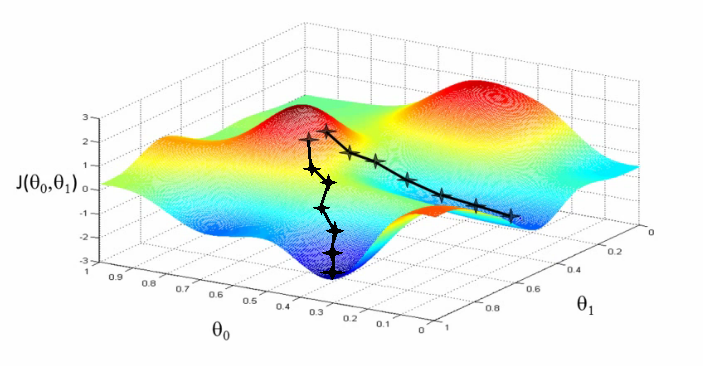
\includegraphics[width=11cm]{figures/localOrGlobalMinimaGD}    % The printed column width is 8.4 cm.
\caption{Gradient descent convergence dependance on $\theta_{init}$. Two different but close choice of $\theta_{init}$ might converge to local or global minima \cite{andrewNg_MachLearning}} 
\label{fig:localOrGlobalMinimaGD}
\end{center}
\end{figure}
 
Learning rate,  $\alpha$, gives the gradient descent its step size, so a bigger value means a faster convergence. 
But keep in mind for a bigger alpha, solution might not converge or even diverge while too small values might lead the optimization to converge very slowly.
A set of $\alpha$ should be tried and evaluated by their performances. A usual set to choose from would be $\alpha = [0.001, 0.01, 0.1, 0.003, 0.03, 0.3]$.
  
Number of iterations, $num\_iter$ is also a parameter to be chosen. 
As a start, conventionally it can be selected as $num\_iter = 1000$ and then, convergence of the cost function should be checked. 
If it has not yet converged but decreasing, a larger value for $num\_iter$ should be selected.

An important point in the algorithm is to update the $\bm{\theta}$ simultaneously. 
So during one iteration, the same $\bm{\theta}$ values should be substituted into $h_\theta(x)$, in order to calculate next values of $\theta_0, \theta_1$.
 
Convergence of gradient descent can be debugged by plotting the cost function as a function of iterations of the optimization.
In the preferred case, the cost function should decrease in each iteration, never increase, and should converge to a steady value at the end of the optimization algorithm. 
Fig.~\ref{fig:visualizeCostFunc} shows two poor and one successful optimization by plotting the cost function versus iteration. 

\begin{figure}[hbt]
\begin{center}
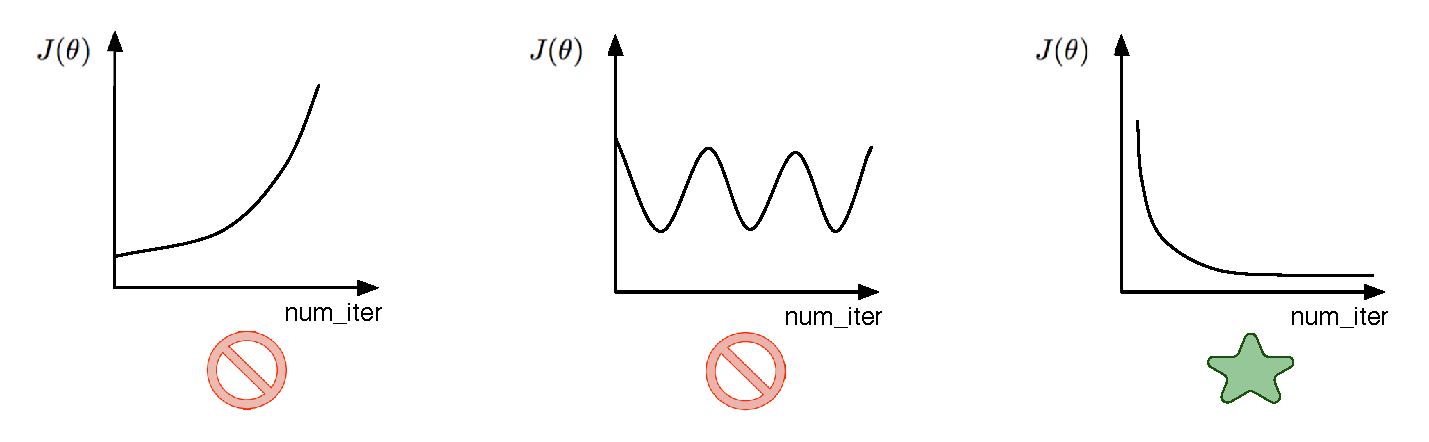
\includegraphics[width=15cm]{figures/visualizeCostFunc}    % The printed column width is 8.4 cm.
\caption{Evolution of $J(\theta)$ with respect to number of iterations. Left two figures showing that the optimization problem is not converging. The figure in the far right is the $J(\theta)$ evolution expected} 
\label{fig:visualizeCostFunc}
\end{center}
\end{figure}

Usually, it is a good practice to declare convergence when $J(\theta)$ decreases by less than $10^{-3}$ in one iteration. 
In case, gradient descent is not converging, a smaller $\alpha$ should be tried. 
But too small values of $\alpha$ could result in a slow convergence. 

And finally, generic gradient descent algorithm for multiple features can be given as below.

 \begin{algorithm}
   \caption{Gradient Descent}
    \begin{algorithmic}[1]
     \Function{GradDes}{$X, y, theta\_init, alpha, num\_iters$}    
           \State \textbf{Inputs:} X - training inputs, \\
           \qquad \qquad y - training outputs, \\
           \qquad \qquad theta\_init - initial guess for the optimized parameter theta,\\ 
           \qquad \qquad alpha - learning rate, \\
           \qquad \qquad num\_iters - number of iterations to find the optimized theta
           \State \textbf{Outputs:} theta - theta\_optimized/ theta vector that minimizes the cost function \\
           \qquad \qquad J - the values of the cost function calculated during the course of iterations
    \State repeat until convergence {
    \State $\theta_j \leftarrow \theta_j - \alpha \frac{\partial}{\partial \theta_j}J(\theta_0, \theta_1, \cdots)$
    	 \State For correct implementation, update simultaneously e.g
	 \State 	\qquad  $temp0 = \theta_0 - \alpha \frac{\partial}{\partial \theta_0}J(\theta_0, \theta_1, \cdots)$
	 \State 	\qquad  $temp1 = \theta_1 - \alpha \frac{\partial}{\partial \theta_1}J(\theta_0, \theta_1, \cdots)$
          \State 	\qquad  \qquad $\vdots$
          \State 	\qquad  $\theta_0 = temp0$
	 \State 	\qquad  $\theta_1 = temp1$
	 \State 	\qquad  \qquad $\vdots$
		 }
       \EndFunction
\end{algorithmic}
\end{algorithm}

\subsubsection{Overfitting}

Overfitting is common for complicated models or decision boundaries with high order polynomial terms as

\begin{equation}{\label{eqn:featureMapping2}}
\bm{x_{mapped}}
=\,
\begin{bmatrix}
1 & x_1 & x_2 & x_1^2 & x_1x_2 & x_2^2 & x_1^3 \cdots & x_1x_2^5 & x_2^6 
\end{bmatrix}
\,^ T
\end{equation} 

If the model is suffering from overfitting, the learnt model might end up fitting very well to the training set, but fail to generalize to the new data during the prediction phase. 
This means that the training set error is not a good predictor for how well the model would predict on new examples.

\begin{figure}
\begin{center}
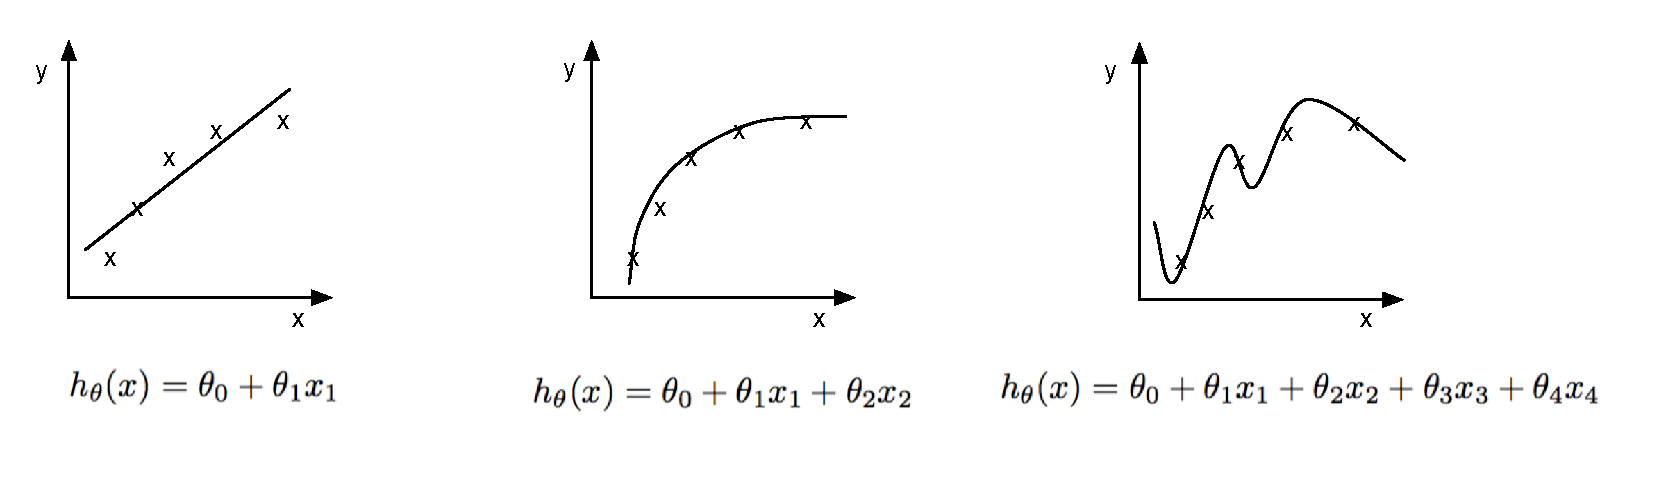
\includegraphics[width=16cm]{figures/underOverFit}    % The printed column width is 8.4 cm.
\caption{Underfitting, just right or overfitting examples - left to right} 
\label{fig:underOverFit}
\end{center}
\end{figure}

Fig.~\ref{fig:underOverFit} show three models where it is easy to realize that the model is underfit, just right or overfit by visualizing the hypothesis. 
But for problems with more features it might not be that obvious. Sometimes it might not even be possible to plot the model to realize if it is overfit or not.
For such cases, methods to detect overfitting should be used. 
To avoid overfitting, regularization parameter is used as explained in the next section.

\textbf{Regularization}

Regularization is practiced to avoid overfitting.
In regularization, a term is added to the cost function in order to penalize parameters $\vec{\bm{\theta}}$ for being large (i.e to make $\vec{\bm{\theta}}$ as small as possible), except ${\theta}_0$ (is not penalized by convention). Cost function for linear regression with the added term for regularization is given as

\begin{equation}{\label{eqn:costFuncRegularized}}
J(\theta)
=\,
\frac{1}{2m} \bigg[ \sum\limits_{i=1}^{m} \Big(h_\theta(x^{(i)}) - (y^{(i)})\Big)^2 +\lambda \sum\limits_{j=1}^{n} \theta_j^2 \bigg] 
\end{equation} 

For logistic regression the regularized cost function can be written as (for two class e.g $y \in \{0,1\}$)

\begin{equation}{\label{eqn:costFuncLogisticRegression}}
J(\theta)
=\,
\frac{1}{m} \sum\limits_{i=1}^{m} \Big[-y^{(i)}log(h_\theta(x^{(i)})) - (1-(y^{(i)}))log(1-h_\theta(x^{(i)}))\Big] +\frac{\lambda}{2m} \sum\limits_{j=1}^{n} \theta_j^2
\end{equation} 

Here, the challenge is to find the appropriate value for $\lambda$ which serves like a weight between the original part of the cost function and the second part, which penalizes $\bm{\theta}$ for being large. 
So it tends to decrease the values of $\theta$. But if this lambda is too big than it then the model converges to  

\begin{equation}{\label{eqn:costFuncRegularizedTooMuch}}
h_\theta(x)
=\,
\theta_0 
\end{equation} 

since all terms are penalized except $\theta_0$ (which is not penalized by convention) such that

\begin{equation}{\label{eqn:costFuncRegularizedTooMuchHow}}
h_\theta(x)
=\,
\theta_0 + \xcancel{\theta_1 x}  + \xcancel{\theta_2 x^2}  + \xcancel{\theta_2 x^3}  + \cdots + \xcancel{\theta_n x^n}
\end{equation} 

Thus the model becomes underfit for large values of $\lambda$, thus should be tuned to acquire the optimal value.


\subsubsection{Visualizing error to diagnose over-fit/under-fit problems}

To further debug the model, a guide is given in Fig.~\ref{fig:debuggingHypothesis}. 
Here, the errors for training and cross validation sets have to be calculated for a variety of polynomial degree or regularization parameter. 
When training and cross-validation errors are plotted as a function of polynomial degree (or complexity of model), a larger training and cross-validation error point toward a under-fit (high bias) model while a large cross-validation and low training error point an over-fit model (high variance) where training and cross validation errors are calculated as in Equ.~\ref{eqn:costFuncTraining} and Equ.~\ref{eqn:costFuncCrossVal}. 
Here, it is assumed that there is no regularization term in the cost function. The training and cross validation errors are calculated in the same way as the cost function since cost function itself is a measure of error.


\iffalse
\begin{equation}{\label{eqn:trainingError}}
J_{training}(\theta)
=\,
\frac{1}{2m} \sum\limits_{i=1}^{m} \Big(h_\theta(x^{(i)}) - y^{(i)}\Big)^2  
\end{equation} 

\begin{equation}{\label{eqn:crossvalError}}
J_{cv}(\theta)
=\,
\frac{1}{2m_{cv}} \sum\limits_{i=1}^{m_{cv}} \Big(h_\theta(x_{cv}^{(i)}) - (y_{cv}^{(i)})\Big)^2  
\end{equation} 
\fi

In the case of the cost function is regularized as given in Equ.~\ref{eqn:costFuncRegularized}, the training and cross validation errors are calculated ignoring the regularization term so they are defined exactly the same as given in Eq. \ref{eqn:costFuncTraining} and Eq. \ref{eqn:costFuncCrossVal} respectively.


Another way to diagnose learning problems is to plot training and cross validation errors with respect to training set size, also named as the learning curves (2 rightmost curves in Fig.~\ref{fig:debuggingHypothesis}). 
Although normally the training set size is constant, here we artificially reduce the number of training examples and calculate the training and cross validation errors. 
For that, the model parameters $\bm{\theta}$ are fit to this reduced training set and then the training and cross validation errors are also calculated over this reduced training data set. 
For the cases where the resulting curves give a low training error and a high cross validation error for smaller training set sizes and also high training and cross validation errors for larger training sizes, the problem is most likely to be suffering from under-fit (high bias). 
Another signature of an under-fit problem is that the training and cross validation errors are similar in magnitude. 
If the learning curves give a low training error and a high cross validation error for the smaller training set size and also training error is increasing with training set size while cross validation error decreasing without leveling off, the problem is more likely to be suffering from overfitting (high variance). 
Another important signature of an over-fit model is that the training error will be less then the cross validation error and the difference in between would remain significant. 

\begin{landscape}
\begin{figure}
\begin{center}
%\includegraphics[width=20cm,angle=90,origin=c]{figures/debuggingHypothesis}    % The printed column width is 8.4 cm.
\includegraphics[width=22cm]{figures/debuggingHypothesis}    % The printed column width is 8.4 cm.
\caption{Diagnosing machine learning problem by plotting training and cross-validation errors} 
\label{fig:debuggingHypothesis}
\end{center}
\end{figure}
\end{landscape}

\subsubsection{Best practices}

After diagnosing the problem is an over-fit or under-fit, those practices is helpful to know. 

To fix a under-fit model, it would help to try 

\begin{itemize}

\item{Adding features}
\item{Adding polynomial features}
\item{Decreasing the regularization term}

\end{itemize}

To fix a over-fit model, it would help to try 

\begin{itemize}

\item{Adding more training examples}
\item{Decreasing the number of features}
\item{Increasing the regularization term}

\end{itemize}

\subsubsection{Prediction}

Finally, for a new set of input data, now output can be predicted using the model/classifier trained. 
One point to remember is that if scaling applied to training set, new data should be scaled as well before being fed to the model/classifier using the same mean and standard deviation values previously calculated from the training set. 
After that, $h(\theta)$ could be evaluated utilizing optimized $\theta$ and scaled new data set $x\_new\_scaled$. 
So $h_\theta(x\_new\_scaled)$ gives

\begin{equation}{\label{eqn:prediction}
h_{\theta}(x\_new\_scaled})
=\,
P\Big(y=1 \, | \, x; \, \theta \Big)
\end{equation} 


which is the probability that $y = 1$ given $x\_new\_scaled$ parametrized by $\bm{\theta}$. 
But still it is important to keep in mind, some other learning methods, the output of the problem could differ, such as the output of an SVM (Support Vector Method) classifier would be directly the class label.


\section{Support Vector Machines}

\subsection{Introduction}

\iffalse Let $ E = \Big\{ \big( \vec{\bm{x}}_1, y_1 \big),\big( \vec{\bm{x}}_2, y_2, 
		\cdots, \big( \vec{\bm{x}}_m, y_m \big) \big) \Big\}$, 
		where $\vec{\bm{x}}_i \in {\rm I\!R}^n$ and $y_i \in \big\{0, 1\big\}$ 
		be a training example set. Assuming the training data linearly separable, 
\fi		

SVM is a relatively new approach for classification offering better generalization property thanks to its foundations on the structural risk minimization principle while other classifiers (such as logistic regression) usually only minimizes the empirical risk \cite{gunn1998support,yin2014study}. This advances the capacity of generalization even with a small number of instances by reducing the risk of overfitting for a nicely tuned parameters setting. It can be applied to nonlinear systems and problems offering a vast number of features. Furthermore, taking advantage of convex optimization problems in the solution of SVM models, another attractive reason to use SVM rises as avoidance of local minimas, while Neural Networks is inherently prone to local minimas.


The aim of SVM is to find an optimal hyperplane maximizing the margin, which is the distance in between the boundaries, by extending them until hitting the first data point as in Fig.~\ref{fig:svmHyperplane}. The points closest to the hyperplane (decision boundary) are called the support vectors and are the representatives of the data sets to be used for the decision process. This helps to decrease the data to handle abruptly, enhancing the ability to cope with the curse of dimensionality and reducing the computational complexity.

\begin{figure}
\begin{center}
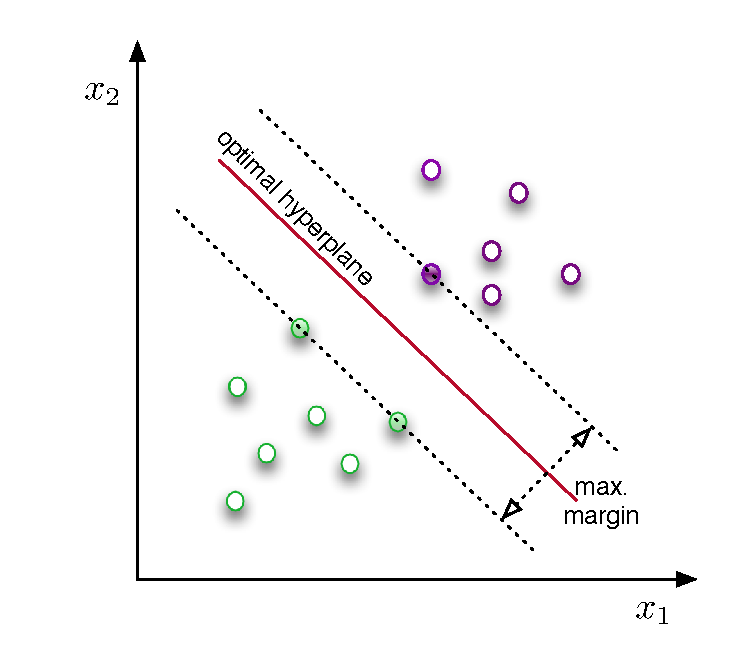
\includegraphics[width=9cm]{figures/svmHyperplane}    % The printed column width is 8.4 cm.
\caption{SVM working principle} 
\label{fig:svmHyperplane}
\end{center}
\end{figure}

SVM implements the idea of having a confidence in the prediction by using the concept of separating data with large margin. 
Some other classification methods, such as logistic regression, output the probability of a new instance's belonging to a particular class, thus inherently give the confidence of the prediction as an output. 
On the other hand, SVM does only output if the new instance's probability of belonging to a particular class, so do not give its confidence on this decision explicitly. 
Rather than including this confidence information as an output in terms of probabilities, this information is introduced with the functional and geometric margins. 
There also exist methods which can be used to calculate the posterior probabilities, which is the probability that the new measurements belongs to its predicted class\cite{platt1999probabilistic}. 
An example of posterior probabilities showing new measurements' probabilities to belong to faulty class is given Fig.~\ref{fig:post_prob}. 

Training data set includes labeled data where the label can belong to one of two possible cases. This data set is saved in a matrix $\bm{X} \in {\rm I\!R^{m \times n}}  $ where $m,n$ correspond to number of instances and features respectively. The label information corresponding to the measurement instances is also fed to the SVM algorithm during the training phase as output vector $\bm{y} \in \{-1,1\}$. The aim of SVM is to find an optimal hyperplane maximizing the margin by solving the optimization problem for non-linearly separable datasets

\begin{align}
min_{\gamma,\omega,b} \quad & \frac{1}{2} \norm{\omega}^2 + C \sum\limits_{i = 1}^m \xi_i \\
s.t. \quad & y^{i}(\omega^T x^(i) + b) \geq 1 - \xi_i, \ i = 1, \cdots, m\\
 & \xi_i \geq 0, \ i = 1, \cdots, m
% hic bir sey yazmazsan esitlikleri alt alta hizaliyor canim benim&=alo \\
% $ tek dolar arasi $ inline denklem
% $$ cift dolar arasi $$ satir atlayarak ortada denklem
\end{align}


Introducing the Lagrange duality to obtain the dual form of the optimization problem, use of kernels, to work efficiently in higher dimensional spaces, is eased. 
The dual form also allows to utilize efficient optimization solvers such as Sequential Minimal Optimization (SMO)  \cite{platt1998sequential} which is the solver used in this work as well. Conventionally, training phase of SVM requires to solve a large quadratic programming (QP) problem. Especially for large training set, computational heaviness of this phase might limit the applicability of SVM to specific problems sets. To overcome this constraint, SMO breaks the QP problem into a series of smaller QP problems which can be solved analytically. 

%Tolerance for the gradient difference between upper and lower violators obtained by Sequential Minimal Optimization (SMO) or Iterative Single Data Algorithm (ISDA), specified as the comma-separated pair consisting of 'DeltaGradientTolerance' and a nonnegative scalar.
% The default values are: 1e-3 if the solver is SMO (for example, you set 'Solver','SMO')

SVM has other tricks to deal with not linearly separable problems such as using kernels to map data into higher dimensional feature spaces where they can be separated with a linear hyperplane. Kernels are at the core of efficient SVM classifiers. A kernel, in general is defined as

\begin{equation}
K (x,z) = {\phi(x)}^T \phi(z)
\end{equation}

where $\phi$ represents the feature mapping. Usually the original features of the systems are named as attributes while the mapped set are called the features. In other words, $\phi$ maps the attributes to the features. Kernels offer various elegant properties such as computational efficiency. 
Cleverly selected, SVM classifiers can learn in high dimensional spaces represented by $\phi$ without the need to explicitly find or represent $\phi$, but instead calculating $K(x,z)$, which might be computationally more efficient. 

 
\subsection{Application}


A binary classifier is used in this work to classify two classes, faulty and nominal. 
SVM being a supervised classification algorithm has two main phases as shown in Fig.~\ref{fig:supervisedLearning}: training and prediction. 


In the training phase, the model is learned to fit the labeled data that is fed to the SVM algorithm. The labeled data set is first divided to two portions with a percentage of 20\%, 80\% where the bigger chunk is the training set and the remaining is the test set. 

This phase is usually followed with a tuning phase where some of the parameters of SVM are changed. Further, the training set is divided as cross-validation and training sets. The idea to split data is to avoid overfitting. When a model is overfit, it fits very accurately to the data it is trained with, but fails to generalize to new data. This results in a poor prediction performance. To avoid overfitting, which is the main problem of parametric discrimination approaches such as neural networks, parameter $C$ is tuned to result in an optimal fit with the cross validation set. Tuning $C$ also gives the user the ability to change the classifier's sensitivity to outliers, since sometimes finding a hyperplane separating all data perfectly is not the favorable option (might cause overfitting). Then the final performance of the classifier is tested on the test set. 

Results are compared to have the best fit via cross validation to avoid overfitting. The last phase is the prediction, where for a new instance, the classifier predicts if it corresponds to a faulty or nominal condition.


The classifier with the best performance is selected and then used in the prediction phase.  
For a new data input, the classifier is used to predict which class the new data belongs to.



\subsubsection{Training of the classifier}

The first step is to normalize the features of the data in order to make the values of features change with the same order of magnitude. 
The reason is due to its benefits to the calculation of parameters of the model via an optimization algorithm and its convergence rate.  
An important point is to keep that values $\mu_j, s_j$ and may be standard deviation if it is used instead of range $s_j$. 
During prediction phase, the data first should be scaled with these values attained from learning data.
If in the model artificial feature  $x_0 = 1$ is added to the features, do not apply scaling to the artificial feature, but this does not apply to SVM classification.

Default settings for SVM binary classification, included in Matlab Statistics and Machine Learning Toolbox, utilizes SMO for optimization if outlier fractions has not been specified during the function call. 

Default settings of Matlab's binary SVM classifier fits a linear model, which results in a linear decision boundary. 
If the system of interest requires a more complicated decision boundary to effectively classify the training data, mapping the original features might be necessary. 

In this study, Gaussian Kernel, which corresponds to an infinite dimensional feature mapping, is utilized to map the attributes.

\begin{equation}
K (x,z) = exp \bigg(-\frac{\Vert x - z \Vert ^ 2}{2 \sigma^2} \bigg)
\end{equation}


\subsubsection{Tuning of the classifier}
% HIGH VARIANCE = OVERFIT =   LARGE C = SMALL sigma^2
% HIGH BIAS = UNDERFIT = SMALL C =  LARGE sigma^2
% sigma^2 LARGE = HIGH BIAS 

Training phase is usually followed by a tuning phase where some of the parameters of SVM are tuned and results are compared in order to have the best fit via cross validation set. This is the phase where the parameters of the classifier are fixed to be used in the last phase, prediction.

\begin{figure}
\begin{center}
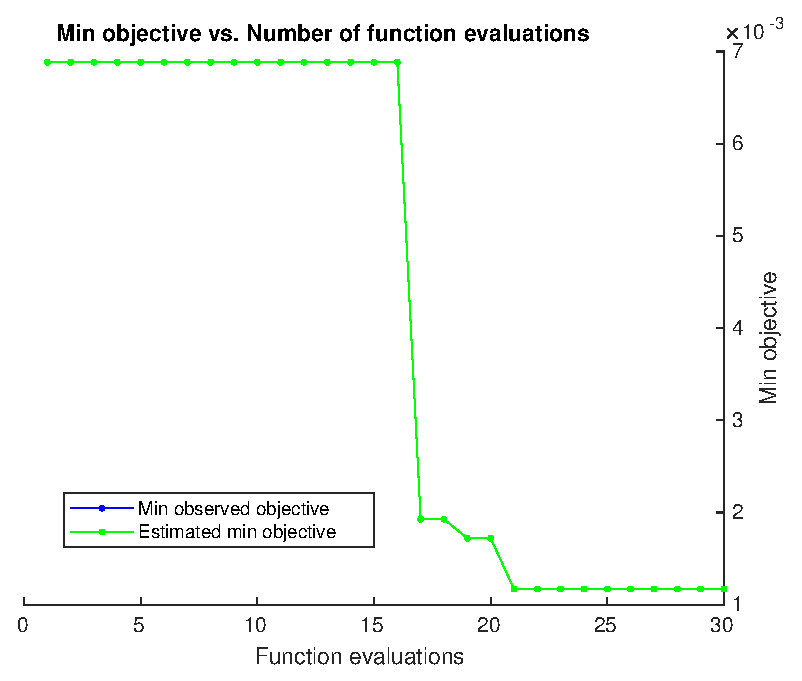
\includegraphics[width=0.7\textwidth]{figures/objectiveFuncEval}    % The printed column width is 8.4 cm.
\caption{Convergence of the objective function} 
\label{fig:objectiveFuncEval}
\end{center}
\end{figure}

To avoiding overfitting, which is the main problem of parametric discrimination approaches such as neural networks, $C$ (box constraint) and the kernel scale (sigma), are tuned.
The classifier is trained with the training set and tuned via cross validation set, and then the selected classifier is evaluated with the test set. Cross-validation set selection of Matlab utilizes a random selection over the data set. 
To compare different methodologies for tuning and also the untuned classifiers, the script has been revised to generate random values from the same seed value to be consistent in comparisons.
Box constraint (C) and kernel scale (sigma) are tuned considering the presence of the outliers to generalize the distribution of the data rather than resulting in fine fits for each individual data in the training set. 

Two different ways are utilized to tune the classifier, heuristic and Bayesian optimization. In heuristic optimization, the strategy is to try a geometric sequence of the kernel scale (sigma parameter) scaled at the original kernel scale.  
Also a geometric sequence of the box constraint parameter, 11 values, from 1e-5 to 1e5 by a factor of 10 have been tried. Increasing box constraint might decrease the number of support vectors, but also might increase training time. 
Usually, increasing box constraint too much induces overfitting (high variance). 

\begin{figure}
\begin{center}
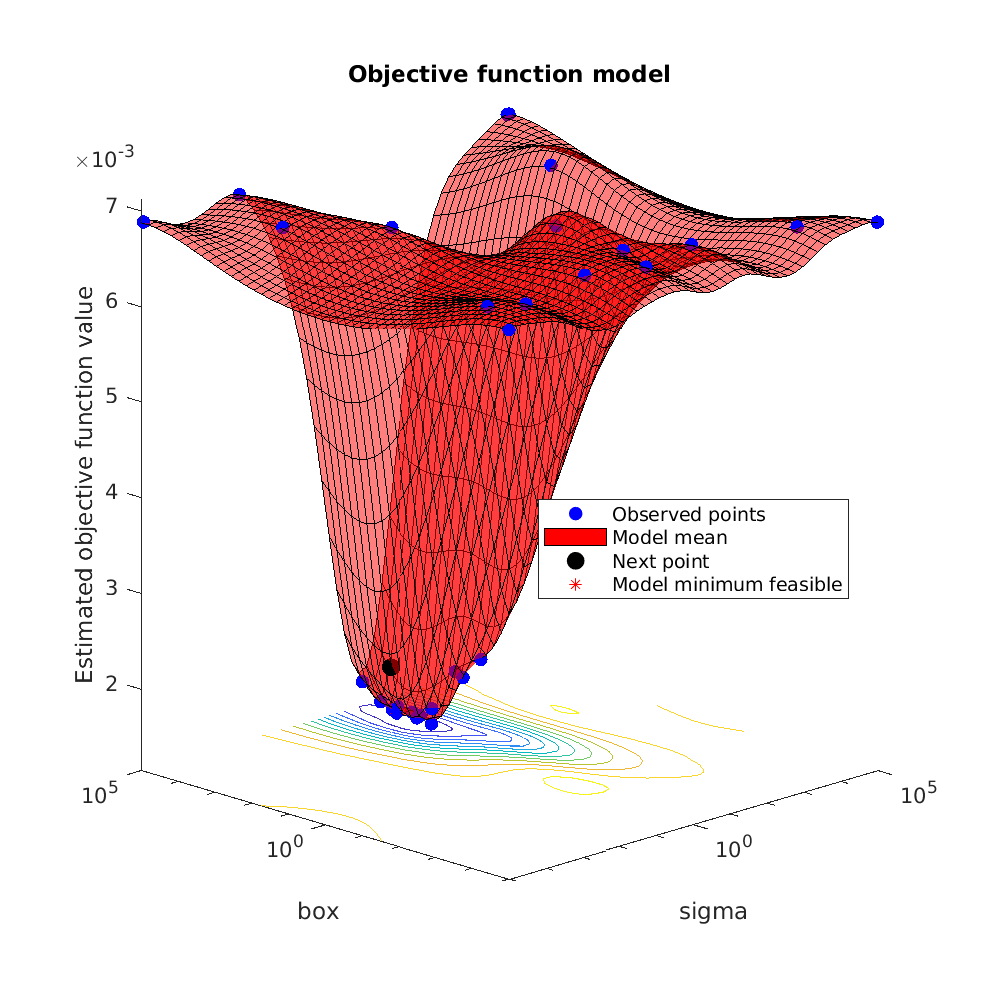
\includegraphics[width=0.7\textwidth]{figures/objFuncModel}    % The printed column width is 8.4 cm.
\caption{Objective function values for different box parameter and sigma values} 
\label{fig:objFuncModel}
\end{center}
\end{figure}


Bayesian optimization tool from Matlab can be used in conjunction with the classification tool to optimize box constraint and the kernel scale. 
This tool outputs minimum objective value as a function of number of function evaluations (max. number of function evaluations can be changed by passing arguments to the function) as shown in Fig. ~\ref{fig:objectiveFuncEval}. 
Fig. ~\ref{fig:objFuncModel} shows the objective function values for a variety of box constraint and kernel scale values. 
The optimized values for box constraint and kernel scale in each iteration are also presented as a table as given in Fig. ~\ref{fig:optBayesianSteps}. 
Also a summary of Bayesian optimization showing the calculated and estimated best values for sigma and box constraint is given at the end of optimization such as Fig. ~\ref{fig:optimBayesianResults}.
With a satisfactory result of the training \& tuning is followed by the prediction where the classifier predicts if the new measurement data belongs to the faulty or nominal class. 

\begin{figure}
\begin{center}
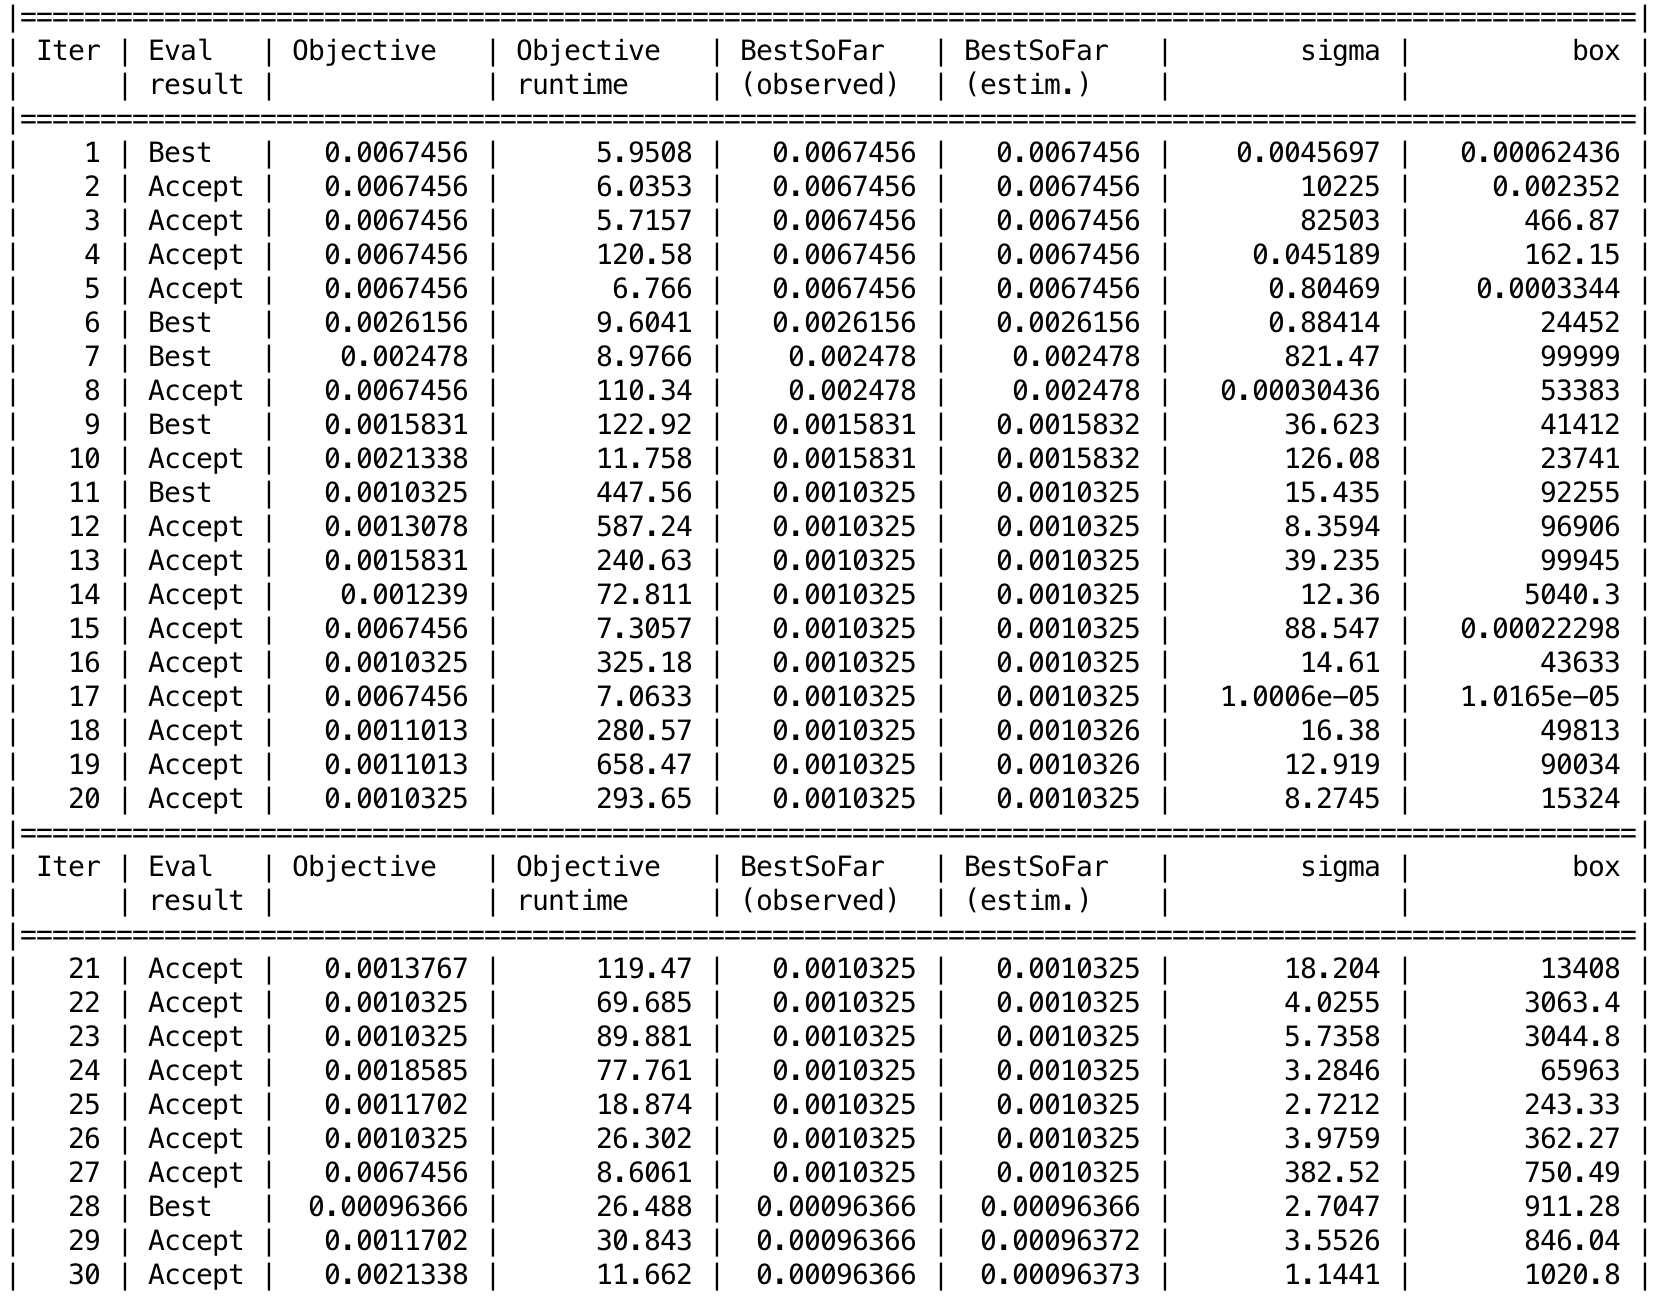
\includegraphics[width=1.13\textwidth]{figures/optimizationSummaryStuckFault}    % The printed column width is 8.4 cm.
\caption{The optimized values for box constraint and kernel scale in each iteration and corresponding value of objective function} 
\label{fig:optBayesianSteps}
\end{center}
\end{figure}

\begin{figure}
\begin{center}
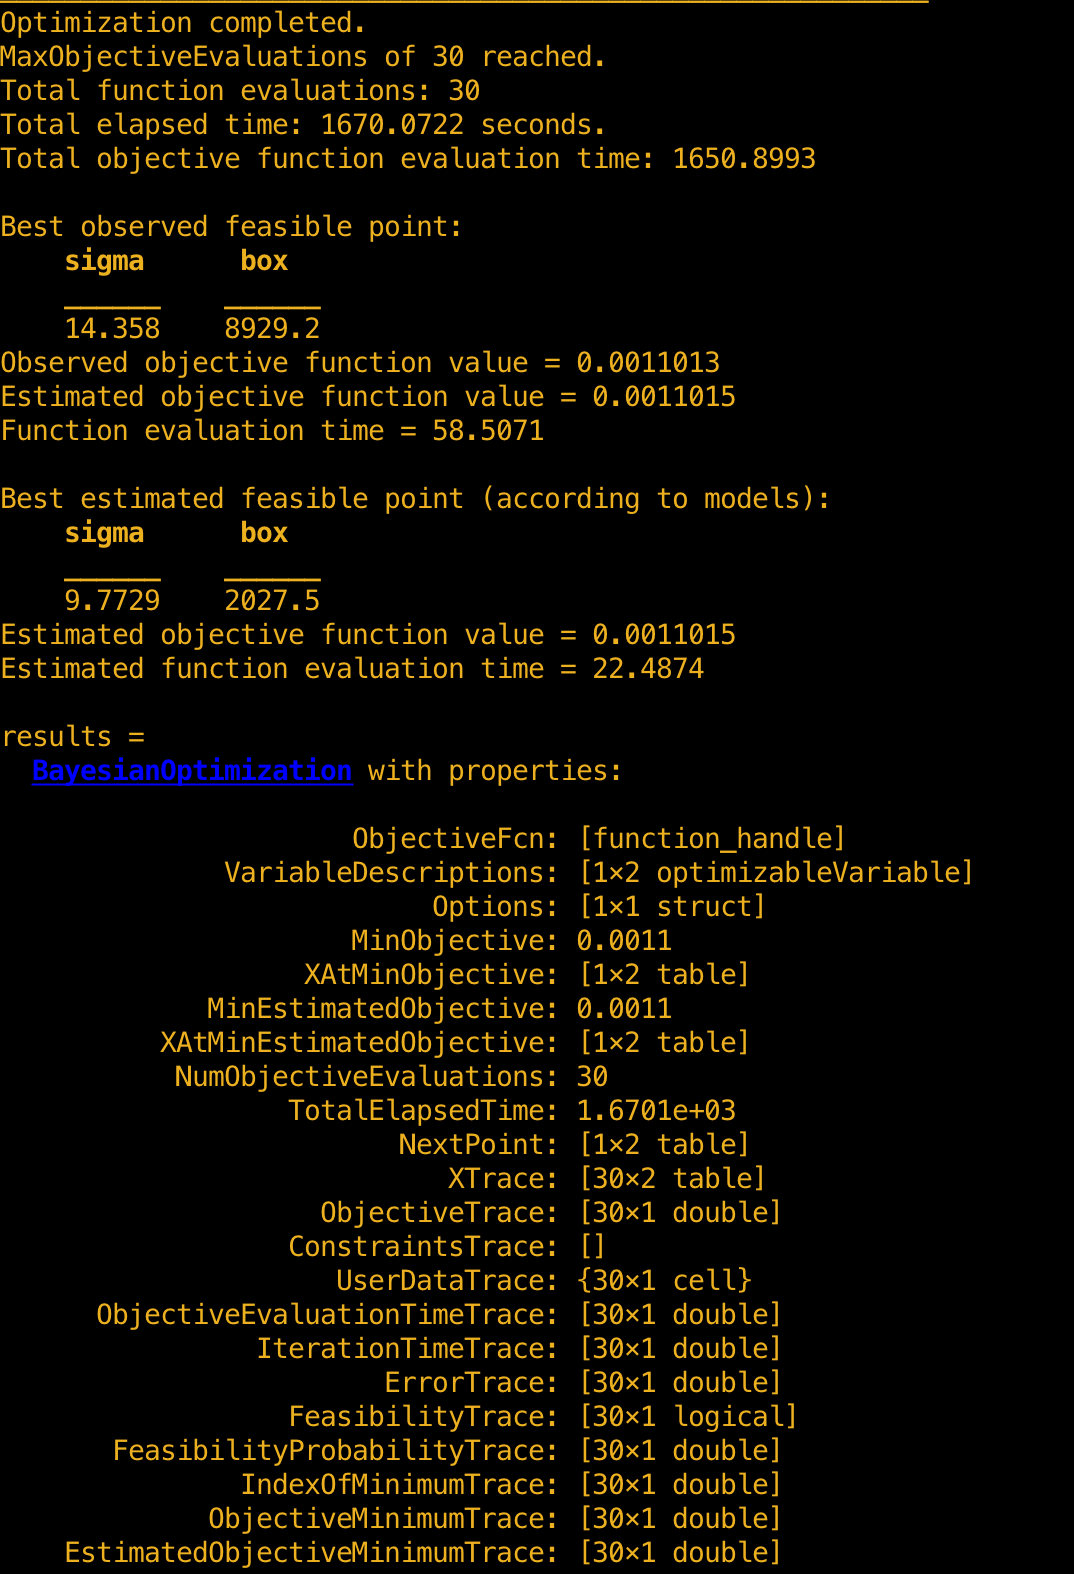
\includegraphics[width=0.6\textwidth]{figures/optimizationResultsStuckFault}    % The printed column width is 8.4 cm.
\caption{Final results for the optimization, time of execution, optimal values of box constraint and sigma values} 
\label{fig:optimBayesianResults}
\end{center}
\end{figure}

\subsubsection{Evaluating the classifier}
\label{evalClassifier}

The performance of the classifier is first quantified by \emph{loss of classification} as indicated with \emph{kFoldLoss} in this work. 
The training data set is  separated to 10 folds. For each fold, the \emph{loss of classification} computed for in-fold observations with a model trained on out-of-fold observations. 
Finally the \emph{loss of classification} is calculated as the \emph{classification error} averaged over all folds.
The idea to split and evaluate the performance of classifiers on different data sets is to avoid overfitting since the fitted classifier would give better results on the data set that it learnt from, but might not generalize well to new data. 
For that reason, both for evaluating the classifiers during tuning phase and finally evaluating the final classifier possessing the tuned parameters, were realized with different data sets.

Another means to evaluate performance of a classifier, available under Matlab Statistics and Machine Learning Toolbox, is via observing the \emph{classification edge}. 
The \emph{edge} is the weighted mean of the \emph{classification margins}. 
Here, the \emph{classification margin} for a binary classifier is defined, for each observation, as the difference between the \emph{classification score} for the \emph{true class} (faulty measurements in the considered problem) and the \emph{classification score} for the \emph{false class} (nominal measurements in the considered problem). 
In this definition, \emph{classification score} is considered as the signed distance from each observation to the decision boundary.

While all these variables would be satisfactory for performance analysis of classifiers, due to the skewed-class nature of the problem, another means of evaluations is necessary.
When the number of instances for different classes in a data set has a big difference, it is named as a skewed-class problem. 
The inherent trickiness to evaluate classifiers for such problems lies on the fact that, predicting only the more frequent class might lead to a misunderstanding that the classifier gives superior performance although it might not be even learning at all. 
For the problem of fault detection of a control surface would serve as a good example to clarify more. 
Since nominal data is not difficult to generate in real flight while it is difficult to fly faulty, the nominal data is much vast compared to the faulty data 

For such problems, in order to define a single metric to evaluate the abilities of classification, \emph{precision} and \emph{recall} should be defined.   
Fig.~\ref{fig:confusionMatrix} shows the confusion matrix which is used to calculate the precision and recall. 
Here, in general, the class indicated by 1 is the skewed class, corresponding to the fault class in this study. 
True positive refers to the number of instances that are predicted faulty and are actually faulty, false positive refers to the number of nominal instances which are miscalculated or predicted as faulty, false negative is the number of instances that are actually faulty but the classifier predicted that they are nominal, and finally the true negative is the number of instances that are predicted as nominal and are actually nominal.
Precision gives a measure on the fraction that was actually faulty of all the measurements that was predicted as faulty. 
Precision can be related to number of false alarms which is cautiously avoided in flight control systems. Precision is defined as 

\begin{figure}
\begin{center}
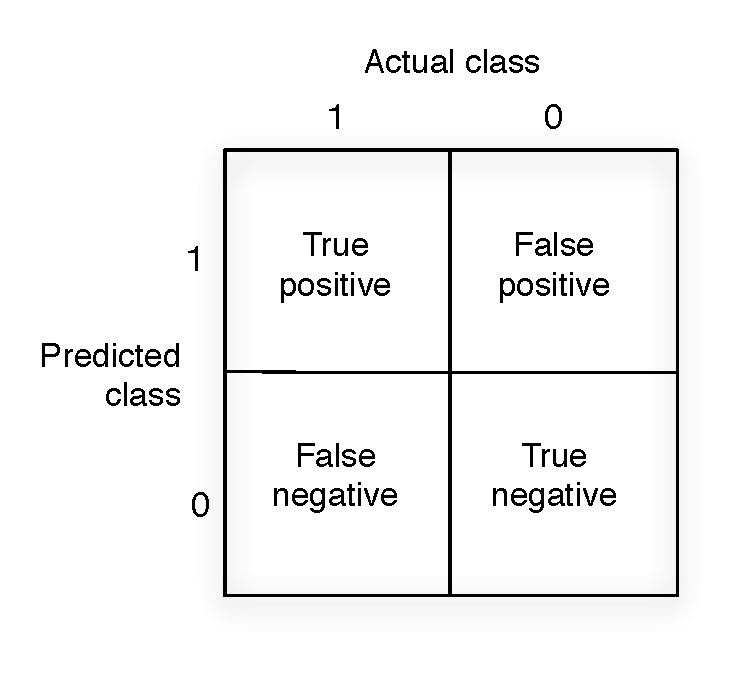
\includegraphics[width=0.5\textwidth]{figures/confusionMatrix}    % The printed column width is 8.4 cm.
\caption{Confusion matrix} 
\label{fig:confusionMatrix}
\end{center}
\end{figure}


\begin{equation}
precision = \frac{true \ positives}{true \ positives + false \ positives}
\end{equation}

Recall refers to the fraction of correctly detected faults of all the situations that was actually faulty. 
Recall can be related to the sensitivity of diagnostic systems. 
Actually an ideal health monitoring system is the one which accomplishes a reasonable balance between the false alarm rate and ability to detect reasonably small faults. 

\begin{equation}
recall = \frac{true \ positives}{true \ positives + false \ negatives}
\end{equation}

Finally as a single metric to evaluate the performance of the classification, F1 score is defined as

\begin{equation}
f1Score = \frac{2 * precision * recall}{precision + recall}
\end{equation}

F1 score, indicated as f1Score in the tables throughout this study is used as the main parameter to evaluate classifiers.

\section{Conclusion}
In this chapter, an introduction to machine learning algorithms is presented. 
Two main branches of machine learning, supervised and unsupervised learning are introduced. 
Terminology and construction of input and output vectors are presented using easy examples of regression and classification. 
Regression and classification are two common problems discussed under supervised learning problem. 
The problems that are frequently encountered during machine learning applications are discussed and best practices to achieve more accurate results are presented. 

After this generic introduction to machine learning implementations, \emph{Support Vector Machines} (SVM) is discussed.  
A very brief section explains its mathematical background and then application procedures are presented.

Next chapter will explain the simulation results by applying SVM to drone flight data. First, results from application of SVM to simulated measurements are presented. Then, SVM is applied to flight data. To be precise on how the data generated, the injection of faults during flight and the modifications to the \emph{Paparazzi} autopilot in order to realize the faults are explained in detail.
%% This is an example first chapter.  You should put chapter/appendix that you
%% write into a separate file, and add a line \include{yourfilename} to
%% main.tex, where `yourfilename.tex' is the name of the chapter/appendix file.
%% You can process specific files by typing their names in at the 
%% \files=
%% prompt when you run the file main.tex through LaTeX.
\chapter{Simulation Results}

This chapter focuses on the results of fault classification simulations under two main sections: classification of faults based on simulated flight measurements and classification of faults based on real flight data. 
In the first part, flight data simulation uses the mathematical equations explained under mathematical modeling chapter of this thesis. 
The second part starts with the explanations on the path to generate faults in real flight thoroughly for two reasons, the importance of having knowledge on data, how it is generated/labeled, and also constructing a guide for researches to realize their own faulty flight campaigns. 
After that, classification for control surface stuck and loss of effectiveness faults have been investigated separately. 

\section{Fault detection from simulated flight data}

In this section, model of an aircraft is simulated in Matlab using the equations of motion given Equ.~\ref{eqn:compactEquOfMotion}. 
This drone model, will not be used for the design of FDD algorithms, but to generate data that will be used by the FDD algorithms. 
After the equations of motion of drone have been solved numerically, accelerometer and gyro measurements have been simulated based on the statistics of the sensors onboard. 
This part of the study uses the model of a MAKO drone to simulate the measurements while the real flights that will be explained in the forthcoming section uses a ZAGI drone.

For MAKO simulation, the stability and aerodynamic force coefficients are generated by AVL. The input vector can be written as $\bm{u}\left(t\right) \in {\rm I\!R} ^3 $
\begin{equation}
\bm{u}\left(t\right)= \begin{bmatrix} {\delta}_{a}\ {\delta}_{e}\ n \end{bmatrix}^{\rm T}
\end{equation}

Here $ \delta_{a}$ aileron deflection angle in degrees, $ \delta_{e}$ elevator deflection angle in degrees, $n$ engine speed in rev/s. 

When the actuators are healthy, actual control input signal will be equal to the given input signal. In case of a fault the actual signal can be modeled as

\begin{equation}
\bm{u}\left(t\right)= \bm{E}\bm{u}_c + u_f
\end{equation}

where $\bm{u}_c $ is the desired control signal, $E = diag(e_1, e_2, e_3)$ is the effectiveness of the actuators where $0 \leq e_i \leq 1 $ with $(i = 1, 2 ,3)$ and $u_f$ additive actuator fault. 
This model makes it possible to simulate all four types of actuator faults shown in Fig.~\ref{fig:actuatorFaults}.

\begin{figure}
\begin{center}
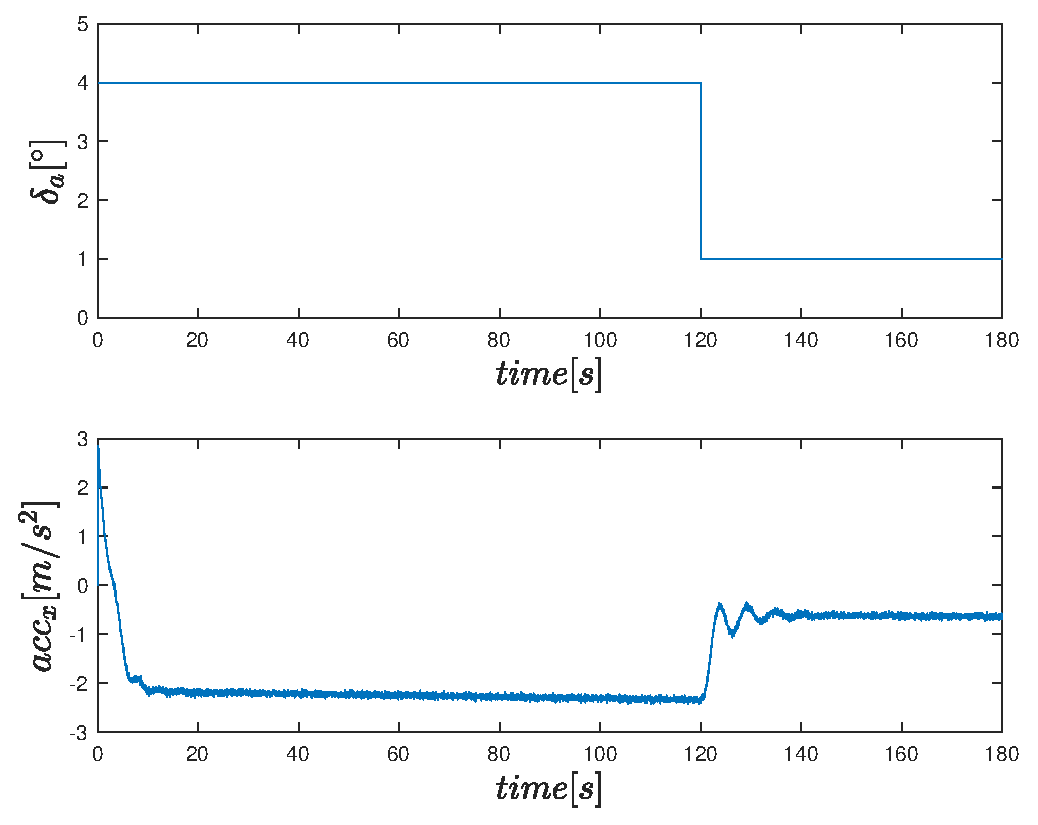
\includegraphics[width=12cm]{figures/control_input_acc_x}    % The printed column width is 8.4 cm.
\caption{Loss of effectiveness fault simulation in aileron command and corresponding accelerometer x axis measurement} 
\label{fig:faultSimulation}
\end{center}
\end{figure}

Most of the FDD algorithms are implemented to open-loop systems, ignoring the probable influences of the controller might cause on the detection performance \cite{pandita2013closed}. Throughout this first section, the system is open-loop as well.  
Here, a step by step approach is followed. In this first section the effect of controller is ignored while in the next section, in which real flight data is utilized, diagnosis is achieved aside a functioning controller.

The code for simulations in this section can be reached in \emph{Github}\footnote{https://github.com/benelgiz/curedRone}. 
First, the measurements are simulated for faulty and nominal flight conditions. 
An example control input in case of loss of efficiency condition could be an actual aileron command of $\delta_{a}^a=1^\circ$ corresponding to a desired $\delta_{a}^d=4^\circ$. In the simulation, the fault is introduced after 120 s. Actual aileron command and corresponding simulated accelerometer $x-axis$ readings can be seen in Fig.~\ref{fig:faultSimulation}. 
The measurements are labeled, and an example plot showing simulated measurements in two-dimensional feature space, $a_x$ - $a_y$, is given as in Fig.~\ref{fig:feat1vsfeat2}. 

\begin{figure}
\begin{center}
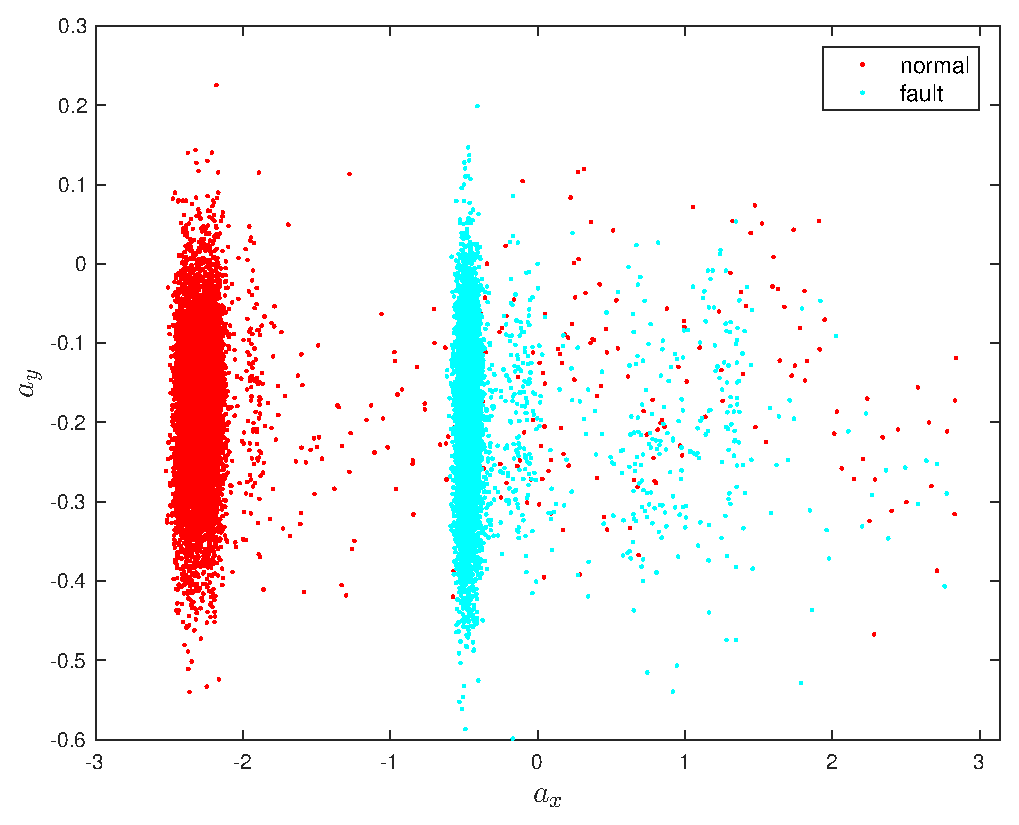
\includegraphics[width=12cm]{figures/feat1vsfeat2}    % The printed column width is 8.4 cm.
\caption{Accelerometer simulation $a_x$ vs $a_y$ } 
\label{fig:feat1vsfeat2}
\end{center}
\end{figure}

%\begin{figure}
%\begin{center}
%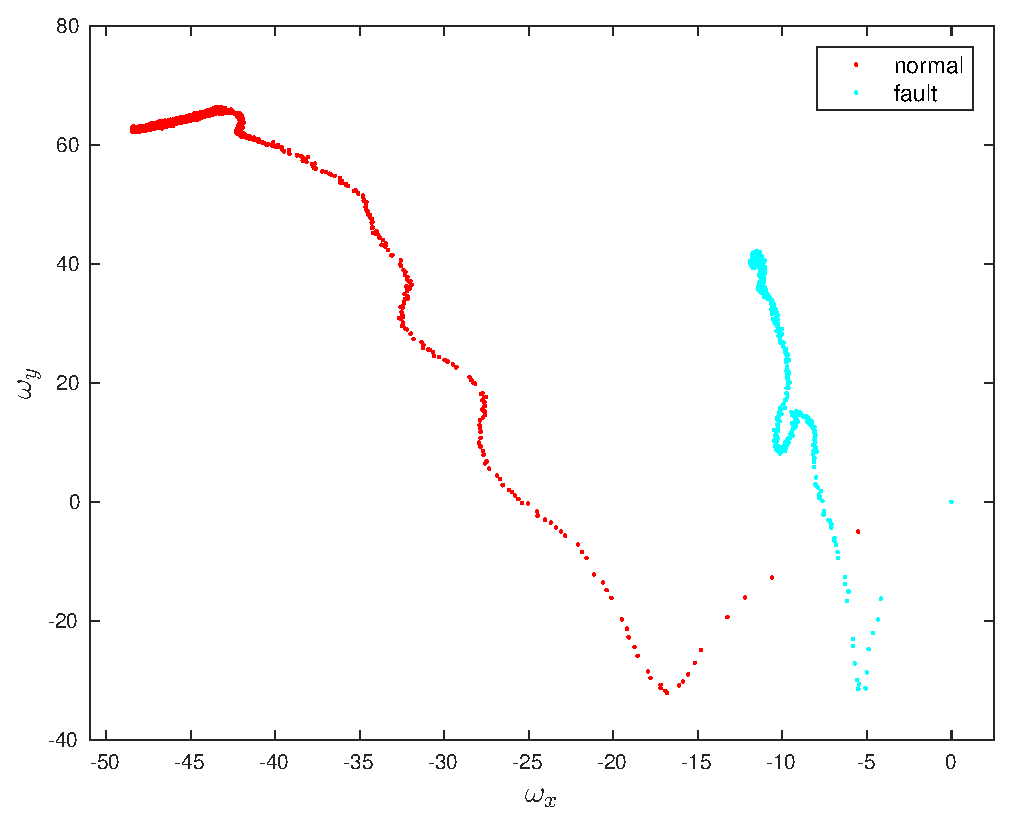
\includegraphics[width=12cm]{figures/feat4vsfeat5}    % The printed column width is 8.4 cm.
%\caption{Accelerometer simulation $a_x$ vs $a_y$ } 
%\label{fig:feat4vsfeat5}
%\end{center}
%\end{figure}

It is always important to visualize the features to have a grasp of data structure before applying machine learning algorithms. 
For that reason, available observations forms the 6-dimensional pattern space,  $\vec{\bm{y}} = \begin{bmatrix} {a_x} & {a_y} & {a_z} & {\omega_x} & {\omega_y} & {\omega_z}  \end{bmatrix}^T$ can be visualized in pairs such as Fig.~\ref{fig:feat1vsfeat2}. 
There are further methods to visualize multidimensional data such as \emph{Tours}\cite{asimov1985grand,cook1997manual,cook1995grand} and \emph{GGobi} data visualization system \cite{cook2007interactive}. In this work, dimensionality reduction technique, Principle Component Analysis (PCA), is utilized for visualization. If very briefly explained, the feature vector $\bm{x}\in{\rm I\!R}^{n}$ is mapped to a lower dimensional space where the 
new feature set will be represented by $\bm{z}\in{\rm I\!R}^{k}$. The final two dimensional feature set can be plotted to give an idea about faulty and nominal measurements' distribution in feature space as shown in Fig.~\ref{fig:z1_vs_z2}.

\begin{figure}
\begin{center}
\includegraphics[width=12cm]{figures/reduceDimMeasurements}    % The printed column width is 8.4 cm.
\caption{Reduced dimensional space features $z_1$ vs $z_2$ } 
\label{fig:z1_vs_z2}
\end{center}
\end{figure}

\begin{figure}
\begin{center}
\includegraphics[width=12cm]{figures/supervisedLearningBasics}    % The printed column width is 8.4 cm.
% For the old picture 
% \includegraphics[width=12cm]{figures/machineLearningBasics}   
\caption{Supervised learning is achieved in two steps: \emph{Training Phase} in which the model parameters are calculated given labeled data and \emph{Prediction Phase} in which the label is predicted for a new input using the trained model.} 
\label{fig:supervisedLearning}
\end{center}
\end{figure}

The aim of machine learning methods is to train a model with a given data set in order to predict the output values corresponding to a new input.
A binary classifier is used in this work to classify two classes, faulty and nominal. 
The fault considered in this study is the loss of effectiveness of the control surfaces. 
SVM being a supervised classification algorithm has two main phases as shown in Fig.~\ref{fig:supervisedLearning}. 
In the training phase, the model is learned as a fit to the labeled data that is fed to the SVM algorithm. 
This phase is usually followed with a tuning phase where some of the parameters of SVM is changed and results are compared to have the best fit via cross validation to avoid overfitting. 
The last phase is the prediction, where for a new instance the classifier predicts if it corresponds to a faulty or nominal condition.

Training data is comprised of labeled data where the label can belong to one of two possible cases. 
This data set is saved in $\bm{X} \in {\rm I\!R^{m \times n}}  $ where $m,n$ correspond to number of instances and features respectively. 
The label information corresponding to the measurement instances is also fed to the SVM algorithm during the training phase as output vector $\bm{y} \in \{-1,1\}$. 
The aim of SVM is to find an optimal hyperplane maximizing the margin by solving the optimization problem for non-linearly separable datasets. For further details on SVM and machine learning in general, the reader could refer to the methodology chapter of this thesis.

\begin{figure}
\begin{center}
\includegraphics[width=11cm]{figures/post_prob}    % The printed column width is 8.4 cm.
\caption{Posterior probability of loss in effectiveness fault for test set when a fault is injected at t = 120s.} 
\label{fig:post_prob}
\end{center}
\end{figure}

To avoiding overfitting, which is the main problem of parametric discrimination approaches such as neural networks, parameter $C$ (box constraint) is tuned to result in the optimal fit for the cross validation set. Box constraint $C$ controls the values of the parameters learnt during the training phase, and further explained under methodology chapter.
The data set available is first divided into two portions with a percentage of \%20, \%80 where the bigger chunk is the training set and the remaining is the test set. 
Further, the training set is divided as cross-validation and training sets. 
The idea to split data is to avoid overfitting. 
Overfitting means that the models trained being very accurate fit for the data they are trained to but fail to generalize with new inputs resulting in bad prediction performance for the new data. 
To improve the performance of the classifier trained with the training data, it is tuned with the cross validation data. 
And finally, ability of the classifier is tested on the test set. 
This parameter also tuned for the outliers to generalize the distribution of the data rather than resulting in fine fits for each individual data in the training set. 
With a satisfactory result of the training \& tuning is followed by the prediction where the classifier predicts if the new measurement data belongs to the faulty or nominal class. 
The output of the SVM classification is not the probability that the new measurement belongs to one class as is in the traditional classification problems, but directly the class information it belongs to. 
For investigating the performance of the classifier on the test set, a method \cite{platt1999probabilistic} is used to calculate the posterior probabilities giving the probability that the new measurements belongs to faulty mode. 
Results shows as in  Fig.~\ref{fig:post_prob} that proper tuning achieves very accurate and instant detection for the drone fault. 
   
%\begin{figure*}
%\begin{center}
%\includegraphics[width=14cm]{modelSelectionNonVisualizableData}    % The printed column width is 8.4 cm.
%\caption{Supervised learning basics } 
%\label{fig:supervisedLearning}
%\end{center}
%\end{figure*}



\section{Fault detection from real flight data}

This second section of the chapter discusses the classification results using real flight data. First, the injection of faults to the flights have been explained throughly. The Paparazzi GCS has been altered to inject real-time faults, controllers in some of flight modes have been changed to accommodate faults. After, the selection of the faults and nominal phases and also labeling data have been presented. Finally, the labeled data have been used to train classifiers for elevon stuck and loss of efficiency faults separately and the classifiers have been evaluated. A variety of techniques implemented to improve the performance such as feature engineering and tuning the classifiers. 

\subsection{Injecting faults in flight from Paparazzi GCS}

For the faulty flight data gathering, some modifications to the \emph{Paparazzi} autopilot was necessary in two main parts: Injecting the faults real-time from GCS, and editing the controller onboard so that the sent faulty input values configures the servos as manipulated from the GCS. 

\begin{figure}
\begin{center}
\includegraphics[width=22cm,angle=90,origin=c]{figures/groundStationFaultInj}    % The printed column width is 8.4 cm.
\caption{View of fault injection tool in Paparazzi ground control station view of in during flight} 
\label{fig:groundStationFaultInj}
\end{center}
\end{figure}

For the former part, a slider is added to the ground station to set the fault during flight and set it back to normal flight conditions if necessary. 
Fig.~\ref{fig:groundStationFaultInj} shows the GCS view with the fault settings open. 
This pane can be found under  \emph{Settings} $>$  \emph{FAULT} as highlighted in pink in Fig.~\ref{fig:groundStationFaultInj}. 
The four row configuration represents from top to bottom, the multiplicative error in the right elevon, the multiplicative error in the left elevon, additive error in the right elevon, and finally the additive error in the left elevon. 
The nominal condition where there is no fault, is given by $[\begin{matrix}right & left & right\_offset &left\_offset\end{matrix}] = [\begin{matrix} 1.0 & 1.0 & 0 & 0\end{matrix}]$. \\
This configuration lets the user to realize all types of actuator faults, such as control surface inefficiency or stuck. 
To generate the fault of right elevon stuck at its nominal position, setting the first slider ($right$) to zero is enough. 
The generate stuck fault at other positions, $right\_offset$ slider should be changed to desired stuck position while keeping the first slider at zero. 

\subsection{Modifications to \emph{Paparazzi} autopilot controls to inject faults during flight}

\begin{figure}
\begin{center}
%\includegraphics[width=17cm]{figures/paparazziControlModes}    % The printed column width is 8.4 cm.
\includegraphics[width=0.9\textwidth]{figures/pprzControlModes}    % The printed column width is 8.4 cm.
\caption{Paparazzi autonomy modes} 
\label{fig:paparazziControlModes}
\end{center}
\end{figure}


For the second part, which is to modify the servo command from the autopilot to the servos, a look at the \emph{Paparazzi} flight modes is necessary. 
Most of the times, there are three modes for fixed-wings from control perspective:  \emph{Auto 1},  \emph{Auto 2},  \emph{Manual}. 
In  \emph{Auto 1}, the pilot is still in the loop and gives the desired pitch and roll values to the controller and the desired elevator and aileron commands are calculated by the autopilot and passed to control allocation where the final desired servo commands are sent to servos as highlighted  \emph{Auto 1} in Fig.~\ref{fig:paparazziControlModes}. 
In the  \emph{Auto 2} mode, there is no need for the pilot since the navigation is also held by the autopilot for a given flight plan. 
This mode is also given as  \emph{Auto 2} in Fig.~\ref{fig:paparazziControlModes}.
In  \emph{Manual} mode, the pilot gives the desired elevator and aileron commands and desired servo commands are calculated in the autopilot's control allocation phase. So still there is a very low sense of autonomy in the manual phase. 

Flying with faults is a challenge. 
The risk to crash is increased on purpose, so a back up plan is necessary to recover from faulty situations if the drone seems to be out of control and/or about to crash. 
For that purpose, the faults are only injected to \emph{Auto} modes and \emph{Manual} mode is always free of faults even a fault is given from the ground station. 
So, when the pilot sees a safety problem during the faulty operation, s/he can switch to \emph{Manual} mode from the remote controller and have the control of the control surfaces free from faults. 
Depending on the nature of the fault injected, such as for some severe stuck control surface fault data gatherings, this might be a game changer since the drone would crash unless an action taken.  
This is shown in Fig. ~\ref{fig:faultInjectionPaparazzi} with a switch initiated by the pilot's remote control. 
This figure shows that during the control allocation phase, which is the calculation of the desired servo commands from given desired elevator/aileron commands, faults are injected if the mode is \emph{Auto 1} and \emph{Auto 2} when fault multiplicative or fault additive values are changed from the GCS by the operator.  When switched to \emph{Manual} mode, the control allocation do not consider the injected faults. 

The modifications in the control allocation code by adding additive and multiplicative faults as well as extracting  \emph{Manual} mode from those injected faults can be seen in the \emph{Paparazzi} code given below. 


\begin{figure}
\begin{center}
\includegraphics[width=0.9\textwidth]{figures/faultInjectionPprz}    % The printed column width is 8.4 cm.
%\includegraphics[width=19cm,angle=90,origin=c]{figures/faultInjectionPaparazzi}    % The printed column width is 8.4 cm.
\caption{Modifications on the control modes of \emph{Paparazzi} autopilot} 
\label{fig:faultInjectionPaparazzi}
\end{center}
\end{figure}


\lstset{language=C}
\begin{lstlisting}

  <command_laws>
    <let var="aileron" value="@ROLL  * AILEVON_AILERON_RATE"/>
    <let var="elevator" value="@PITCH * AILEVON_ELEVATOR_RATE"/>
    <let var="manual" value="(fbw_mode==FBW_MODE_MANUAL)"/>
    <let var="vfault_left" value="100 * ($manual ? 1 : fault_left)"/>
    <let var="vfault_right" value="100 * ($manual ? 1 : fault_right)"/>
    <let var="vfault_offset_left" value="($manual ? 0 : fault_offset_left)"/>
    <let var="vfault_offset_right" value="($manual ? 0 : fault_offset_right)"/>
    <set servo="MOTOR" value="@THROTTLE"/>
    <set servo="AILEVON_LEFT" value="(($elevator - $aileron) * $vfault_left) / 100 + $vfault_offset_left"/>
    <set servo="AILEVON_RIGHT" value="(($elevator + $aileron) * $vfault_right) / 100 + $vfault_offset_right"/>
  </command_laws>
  
\end{lstlisting}


\subsection{Reading \& labeling flight data}


Flight data saved to the SD card onboard should be converted to \emph{.data} format by using the \textit{sd2log} program of \emph{Paparazzi}. For that purpose, from the terminal, browse into the folder including  the .LOG file, which is the file format for the onboard data saved in Paparazzi. 

\begin{figure}[h]
\begin{center}
\includegraphics[width=15cm]{figures/dataManip}    % The printed column width is 8.4 cm.
\caption{Conversion of raw flight data saved to SD card onboard to .data file to be used in further calculations} 
\label{fig:dataManip}
\end{center}
\end{figure}

Run the program under paparazzi/sw/logalize/sd2log and specify the file is to be converted to \emph{.data} file and where to export it as shown in Fig.~\ref{fig:dataManip} ('.' means extract to current folder). 

An example of a part of the flight data\footnote{17\_07\_06\_\_10\_21\_07\_SD.data} is given in Fig.~\ref{fig:dataSettingsNominalFault} and whole file is available in \emph{Github}\footnote{https://github.com/benelgiz/cureDDrone/tree/master/ \\ data/v4\_multiplicativeAdditive\_MURET\_06\_07\_2017}. 
The UAV used to realize the faulty flights in order to generate labeled data is given in Fig.~\ref{fig:zagi}. 

\begin{figure}[h]
\begin{center}
\includegraphics[width=0.87\textwidth]{figures/zagi}    % The printed column width is 8.4 cm.
\caption{The flying-wing: \emph{ZAGI}} 
\label{fig:zagi}
\end{center}
\end{figure}

The duration of the flight was around an hour. 
The flight has been practiced under strong wind. 
34 different faults are injected.
During the flight, the effect of the faults on the drone was sometimes visible to human eye and sometimes not. 
For the control surface stuck faults, even for one control surface was stuck case, it immediately gets out of control and safety pilot takes the initiative. 
Thanks to the piloting skills, no crashes occurred. 
For ineffectiveness of control surface faults, where the controller has still an effect but not as efficient as before, error in navigation was observed.  

\begin{figure}
\begin{center}
\includegraphics[width=11.9cm]{figures/dataSettingsNominalFault}    % The printed column width is 8.4 cm.
\caption{A small part of the flight data corresponding to nominal and two different fault phases of the flight. \emph{Settings} message exists only if there is a change in the multiplicative and additive fault parameters via GCS} 
\label{fig:dataSettingsNominalFault}
\end{center}
\end{figure}


Now that the \emph{.data} file is ready, next is to detect the time stamps at which the faults are injected and then label all the data corresponding to this fault interval as designated with different colors in Fig.~\ref{fig:dataSettingsNominalFault}. 
Since, most of the times, there has been more than one fault type generated during flights, another step in data manipulation is to choose the faults to investigate. 

The fault injection or change from fault condition to nominal mode is done via the GCS and there is a corresponding message saved to SD card onboard in \emph{Paparazzi} \emph{Messages} indicated via \emph{Settings}. 
\emph{Settings} gives multiplicative fault and additive fault values and only appears in the flight data when one of the control surface effectiveness values is changed. 
The value of the \emph{Settings} for nominal phase is [1.0 1.0 0.0 0.0] and a corresponding example line in the data corresponding to a command to revert to nominal condition can be seen in Fig.~\ref{fig:flightDataSettings}. 

\begin{figure}[h]
\begin{center}
\includegraphics[width=13cm]{figures/flightDataSettings}    % The printed column width is 8.4 cm.
\caption{\emph{SETTINGS} \emph{Message} saves the multiplicative and additive fault values inserted from the GCS.  [1.0 1.0 0.0 0.0] corresponds a command from the GCS to revert back to nominal phase} 
\label{fig:flightDataSettings}
\end{center}
\end{figure}

It means to multiply the value given by the controller by 1 and add 0, so does not change the values given by the autopilot. 
As soon as any of control surface effectiveness values is changed in the GCS, a new \emph{Settings} value is saved to the file (Shown with arrows in Fig.~\ref{fig:dataSettingsNominalFault}). 

To find the indexes where the nominal and faulty data starts and ends, the values of the  \emph{Settings} message is investigated. 
So when there is a  \emph{Settings} message in the flight, it should be either a fault generation or going back to nominal condition after a fault. 
If the message contains the  \emph{Settings} message equal to [1.0 1.0 0.0 0.0], this data index is selected as the nominal condition start index and a previous index before next  \emph{Settings} message is the last index of this nominal phase. 
The matrix holding the start and end index for the nominal phases are saved as \textit{nominal\_start\_stop} shown in Table~\ref{arm:tableNominalindexes} where the first row corresponds to start index of each nominal set and second row corresponds to the last index of the corresponding as nominal phase. 

\newcolumntype{M}[1]{>{\centering\arraybackslash}m{#1}}

\begin{table}
\caption{Nominal phase start stop indexes of the flight}
\label{arm:tableNominalindexes}
\begin{center}
\begin{tabular}{ ||m{4.7cm}|m{1.3cm}|m{1.3cm}|m{1.3cm}|m{1.3cm}|m{1.3cm}|m{1.3cm}|m{1.3cm}|m{1.3cm}|m{1.3cm}|m{1.3cm}|m{1.3cm}||}\hline
\textbf{nominal phase number} & 2 & 3 & 4 & 5 & $\cdots$ & 12 \\\hline
\vtop{\hbox{\strut \textbf{nominal start }}\hbox{\strut \textbf{nominal\_start\_stop(1,:)}}} & 516919 & 551627 & 755227	& 824545	& $\cdots$ & 1048055 \\\hline
\vtop{\hbox{\strut \textbf{nominal stop}}\hbox{\strut \textbf{nominal\_start\_stop(2,:)}}} & 521965 & 622015 & 782580 & 924704 & $\cdots$ & 1065548 \\\hline
\end{tabular}
\end{center}
\end{table}

For the fault indexes a similar approach is followed except that  \emph{Settings} messages selected are the ones which is different than  [1.0 1.0 0.0 0.0]. 
An example is Fault \#23 in Fig.~\ref{fig:settingsStuckFault} and its corresponding start and end indexes given in Table~\ref{arm:tableFaultyindexes}.

\begin{figure}[h]
\begin{center}
\includegraphics[width=11cm]{figures/settingsStuckFault}    % The printed column width is 8.4 cm.
\caption{SETTINGS message corresponding to stuck of right control surface} 
\label{fig:settingsStuckFault}
\end{center}
\end{figure}

\newcolumntype{M}[1]{>{\centering\arraybackslash}m{#1}}

\begin{table}[h]
\caption{Faulty phase start stop indexes of the flight}
\label{arm:tableFaultyindexes}
\begin{center}
\begin{tabular}{ ||m{4.7cm}|m{1.3cm}|m{1.3cm}|m{1.3cm}|m{1.3cm}|m{1.3cm}|m{1.3cm}|m{1.3cm}|m{1.3cm}|m{1.3cm}|m{1.3cm}|m{1.3cm}||}\hline
\textbf{fault phase number} & 1 & 2 &  $\cdots$ & 23 & $\cdots$ & 34 \\\hline
\vtop{\hbox{\strut \textbf{fault start }}\hbox{\strut \textbf{fault\_start\_stop(1,:)}}} & 456888 & 473827 & $\cdots$	& 924705	& $\cdots$ & 1076847 \\\hline
\vtop{\hbox{\strut \textbf{fault stop}}\hbox{\strut \textbf{fault\_start\_stop(2,:)}}} & 473826 & 485762 & $\cdots$ & 925390 & $\cdots$ & 1077117 \\\hline
\end{tabular}
\end{center}
\end{table}


Next step is to choose the phases of the flight to work with. 
As an example, a phase of the flight where there is enough nominal data and followed with an extreme fault injection is selected. 
This corresponds to the 4th nominal phase of the flight followed by the 23th fault is selected. Fault \#23 corresponds to right control surface stuck and can be seen in  Fig.~\ref{fig:dataSettingsNominalFault}. 
The next is to select the measurement corresponding the these selected time intervals and this is done by AND ing the indexes of interest, such as the indexes of fault and gyro data measurements as shown in Fig.~\ref{fig:labelingGyroAccel}. 
The script for labeling the nominal and faulty measurements is the \emph{selectDataToInvest.m} file given in Appendix B.2. 
The output of this file is the accelerometer and gyro measurements corresponding to selected phases of the flight.

\begin{figure}[h]
\begin{center}
\includegraphics[width=15cm]{figures/labelingGyroAccel}    % The printed column width is 8.4 cm.
\caption{Indexing SETTINGS, to find fault and nominal flight intervals, indexing GYRO measurements to AND with FAULT indexes to find the indexes of faulty gyro measurements} 
\label{fig:labelingGyroAccel}
\end{center}
\end{figure}

SVM classifier has been trained and tuned with the flight data, generated by following the steps covered above, in order to classify the faulty and nominal classes.
The simulations have been developed under Matlab coding environment. 
Some tools, such as calculation of \emph{f1Score}, were written as Matlab scripts rather than changing some arguments of toolbox functions, since they were not found available in the toolbox either it does not exist or was difficult to obtain.
 
 The simulations have been executed on HP Z820 Workstation with 3.1 GHz, 32 cores. 
 
This work investigates only binary classification, not multi-class classification considering multiple different faults.  
But different faulty cases have been studied to further attack the problem of multi-class classification in the future studies. 
The classifier's abilities in different fault conditions have been investigated. 
The main two types of faults of interest in this study were control surface stuck and LOE. 
The flight data\footnote{https://github.com/benelgiz/cureDDrone/tree/master/ \\ data/v4\_multiplicativeAdditive\_MURET\_06\_07\_2017} and code\footnote{https://github.com/benelgiz/cureDDrone/tree/master} that has been developed are publicly available under \emph{Github}.

All three steps (training, tuning and evaluation), explained thoroughly under SVM application section have been applied and the results are given below.

\subsection{Control surface stuck fault}

During the flights, the most challenging fault to realize was the control surface stuck. 
The drone reacted very fast with an uncontrollable dive towards the ground and the safety pilot initiated manual recovery by triggering the safety switch shown in Fig.~\ref{fig:faultInjectionPaparazzi}. 
So the time past starting from the ignition of the control surface stuck fault until the manual pilot's intervention is very short ($\sim$2 seconds) which can be seen from the accelerometer x-direction readings in Fig.~\ref{fig:acc_x}. 


\begin{figure}[h]
\begin{center}
\includegraphics[width=0.7\textwidth]{figures/acc_x}    % The printed column width is 8.4 cm.
\caption{Accelerometer readings along $x$-direction during flight interval just before control surface stuck (nominal, represented with blue) and during control surface stuck at $\SI{0}{\degree}$ until the safety pilot's intervention} 
\label{fig:acc_x}
\end{center}
\end{figure}

This causes the problem of skew-class classification where there is a big difference between the number of instances belonging to different classes and requires some special treatment as explained above under section ~\ref{evalClassifier}.

First problem considered for classification is the right elevon stuck at $\SI{0}{\degree}$.
Gyro and accelerometer measurements are saved to SD card onboard at 60 Hz. 
Nominal class involves $\sim$5 minutes of accelerometer and gyro data while the faulty class comprised of $\sim$2 seconds of data, thus the problem is treated as skew-class classification. 

Having knowledge about data is critical for machine learning applications. 
Usually, the performance of the learning algorithms are quite dependent on the level of the engineer's experience since some of the critical decision are handled by her/him such as selection of features (not for all machine learning methods).
Fig.~\ref{fig:acc_x} shows accelerometer x-axis measurements for a duration of $\sim$20 seconds. 
Measurements plotted in blue indicates the part of the flight where elevon works correctly while red part of the plot corresponds to the faulty phase. 
It can be interpreted from the Fig.~\ref{fig:acc_x} that the fault injected shows a distinct change in the x-axis accelerometer measurements when the fault is injected. 

%\begin{figure}
%\begin{center}
%\includegraphics[width=11cm]{figures/acc_y}    % The printed column width is 8.4 cm.
%\caption{$a_x$ vs $a_y$ feature space for faulty nominal flight data} 
%\label{fig:acc_y}
%\end{center}
%\end{figure}

%\begin{figure}
%\begin{center}
%\includegraphics[width=11cm]{figures/acc_y_longNominal}    % The printed column width is 8.4 cm.
%\caption{$a_x$ vs $a_y$ feature space for faulty nominal flight data} 
%\label{fig:acc_y_longNominal}
%\end{center}
%\end{figure}

\begin{figure}
\begin{center}
\includegraphics[width=0.66\textwidth]{figures/acc_x_evenLongerNominal}    % The printed column width is 8.4 cm.
\caption{Accelerometer readings along $x$-direction during flight interval before control surface stuck (nominal, represented with blue) and during control surface stuck at  $\SI{0}{\degree}$ until the safety pilot's intervention} 
\label{fig:acc_x_evenLongerNominal}
\end{center}
\end{figure}


To investigate further, measurements have been plotted during a larger time scale involving $\sim$70 seconds of measurements as shown in Fig.~\ref{fig:acc_x_evenLongerNominal}. 
Here, it is seen that the accelerometer measurements corresponding to faulty phase could be observed during the nominal flight phase as well, thus it might be necessary to check the time change of translational acceleration to catch a difference in behavior. 

\begin{figure}[!h]
\begin{center}
\includegraphics[width=0.66\textwidth]{figures/acc_z}    % The printed column width is 8.4 cm.
\caption{Accelerometer measurements along z direction $a_z$ for faulty and nominal flight data} 
\label{fig:acc_z}
\end{center}
\end{figure}

\begin{figure}[h]
\begin{center}
\includegraphics[width=0.65\textwidth]{figures/gyro_x}    % The printed column width is 8.4 cm.
\caption{Angular velocity $w_x$  for faulty nominal flight data} 
\label{fig:gyro_x}
\end{center}
\end{figure}

Fig.~\ref{fig:acc_z} and Fig.~\ref{fig:gyro_x} show the accelerometer measurements along z-direction and angular velocities along x-direction during a short time interval. 
Here, although an average of faulty measurements would result in an obvious difference, individual measures might correspond to nominal phase of the flight as well.

\begin{figure}[!h]
\begin{center}
\includegraphics[width=0.65\textwidth]{figures/feat1vsfeat3FaultStuck}    % The printed column width is 8.4 cm.
\caption{$a_x$ vs $a_z$ feature space for faulty nominal flight data} 
\label{fig:feat1vsfeat3FaultStuck}
\end{center}
\end{figure}

\begin{figure}[h]
\begin{center}
\includegraphics[width=0.65\textwidth]{figures/feat1vsfeat2FaultStuck}    % The printed column width is 8.4 cm.
\caption{$a_x$ vs $a_y$ feature space for faulty nominal flight data} 
\label{fig:feat1vsfeat2FaultStuck}
\end{center}
\end{figure}

%\begin{figure}
%\begin{center}
%\includegraphics[width=11cm]{figures/acc_z_longNominal}    % The printed column width is 8.4 cm.
%\caption{$a_x$ vs $a_y$ feature space for faulty nominal flight data} 
%\label{fig:acc_z_longNominal}
%\end{center}
%\end{figure}

The measurements are also plotted in feature spaces $a_x$-$a_z$ and $a_x$-$a_y$ as shown in Fig.~\ref{fig:feat1vsfeat3FaultStuck} and Fig.~\ref{fig:feat1vsfeat2FaultStuck}. 
It shows $a_x$-$a_z$ space gives a distribution that would be easier to classify the faulty and nominal phases while in $a_x$-$a_y$ feature space, the measures are quite similar and difficult to classify.

\begin{table}[!ht]
	\centering
% table caption is above the table
\caption{Untuned and tuned via heuristic approach and tuned via Bayesian optimization SVM classification evaluations}
\label{tab:stuck}       % Give a unique label
% For LaTeX tables use
\begin{tabular}{p{2.7cm}p{2.0cm}p{2.3cm}p{3cm}p{3cm}}
\hline\noalign{\smallskip}
 & Untuned linear kernel & Untuned Gaussian kernel & Tuned heuristic Gaussian kernel & Tuned Bayesian Gaussian kernel\\
\noalign{\smallskip}\hline\noalign{\smallskip}
kernel scale & 1 & 1 & 2.1187 & 10.3581 \\
box constraint & 1 & 1 & 1 & 1323.1 \\
margin & 10.5927 & 2.0248 & 2.4763 & 5.3004 \\
edge & 10.5875 & 2.0245 & 2.4761 & 5.3004 \\
kFoldLoss & 0.2 x $10^{-2}$ & 1.2 x $10^{-3}$& 7.571 x $10^{-4}$ & 1.2 x $10^{-3}$ \\
precision & 0.76 & 1 & 1 & 0.913 \\
recall & 0.8261 & 0.8696 & 0.913 & 0.913\\
\textbf{f1Score} & 0.7917 & 0.9302 &0.9545 & 0.913 \\
comp. time & 3.75s & 3.4s & 5917.5s & 1784.7s \\
\noalign{\smallskip}\hline
\end{tabular}
\end{table}

%\begin{figure}
%\begin{center}
%\includegraphics[width=11cm]{figures/gyro_x_longNominal}    % The printed column width is 8.4 cm.
%\caption{$a_x$ vs $a_y$ feature space for faulty nominal flight data} 
%\label{fig:gyro_x_longNominal}
%\end{center}
%\end{figure}

%\begin{figure}
%\begin{center}
%\includegraphics[width=11cm]{figures/gyro_y}    % The printed column width is 8.4 cm.
%\caption{$a_x$ vs $a_y$ feature space for faulty nominal flight data} 
%\label{fig:gyro_y}
%\end{center}
%\end{figure}

%\begin{figure}
%\begin{center}
%\includegraphics[width=11cm]{figures/gyro_y_longNominal}    % The printed column width is 8.4 cm.
%\caption{$a_x$ vs $a_y$ feature space for faulty nominal flight data} 
%\label{fig:gyro_y_longNominal}
%\end{center}
%\end{figure}

%\begin{figure}
%\begin{center}
%\includegraphics[width=11cm]{figures/gyro_z}    % The printed column width is 8.4 cm.
%\caption{$a_x$ vs $a_y$ feature space for faulty nominal flight data} 
%\label{fig:gyro_z}
%\end{center}
%\end{figure}

%\begin{figure}
%\begin{center}
%\includegraphics[width=11cm]{figures/gyro_z_longNominal}    % The printed column width is 8.4 cm.
%\caption{$a_x$ vs $a_y$ feature space for faulty nominal flight data} 
%\label{fig:funcEval1}
%\end{center}
%\end{figure}


Table~\ref{tab:stuck} shows the results of SVM classification for untuned linear kernel, untuned Gaussian kernel, and tuned Gaussian kernel via two methods (heuristic and Bayesian) respectively in its columns.  
Although a variety of variables used in the evaluation of classifiers have been presented to the reader for completeness, f1Score will be the main variable of concern for this study for the reasons explained before. 
The classifier with a \emph{box constraint} $= 2.11$ and a \emph{kernel scale} $ = 1$ have been found to give the highest \emph{f1Score} (\emph{f1Score} $= 0.9545$). 

Due to previous observations on data, feature set have been widened via additions of data from past measurements for each attribute. 
The idea is to introduce the time change behavior of data to be represented in each instance. 
The number of features have been increased to 24 in Table~\ref{tab:contSurfStuckAddedFeat}, which means only 3 previous measures for each different attribute have been added to the feature set ((3 past + 1 instant) * 6 axis).
This addition to the feature set, in general, deteriorated the performance of the classifier, especially the classifier with an untuned Gaussian kernel (\emph{f1Score}= $0.4167$) ($\Delta f1Score = -0.5135$). 
For the classifiers with tuned Gaussian kernels, \emph{f1Score} decreases by a small amount for the classifier tuned with heuristic method (\emph{f1Score} $= 0.9444$) and increases by an even smaller amount(\emph{f1Score} $= 0.9143$) hence the effect is not really obvious. 


% For tables use
\begin{table*}[h]
	\centering
% table caption is above the table
\caption{Untuned and tuned via heuristic approach and tuned via Bayesian optimization SVM classification evaluations}
\label{tab:contSurfStuckAddedFeat}       % Give a unique label
% For LaTeX tables use
\begin{tabular}{p{2.6cm}p{2cm}p{2.5cm}p{2.7cm}}
\hline\noalign{\smallskip}
 & Untuned \ 24 features & Tuned Heuristic 24 features & Tuned Bayesian Opt. 24 features\\
\noalign{\smallskip}\hline\noalign{\smallskip}
kernel scale & 1 & 6.0609 & 67.33 \\
box constraint & 1 & 10 &  47330\\
margin & 1.9733 & 3.6353 & 5.6484 \\
edge & 1.9678 & 3.6317 & 5.6404 \\
kFoldLoss & 5.6 x $10^{-3}$ & 3.44 x $10^{-4}$ & 6.19 x $10^{-4}$ \\
precision & 1 & 1 & 1 \\
recall & 0.2632 & 0.8947 & 0.8421\\
\textbf{f1Score} & 0.4167 & 0.9444 & 0.9143 \\
comp. time & 12.4s & 5581.9s &1205.2s \\
\noalign{\smallskip}\hline
\end{tabular}
\end{table*}

% Second trial for the same number of features
% For tables use
\begin{sidewaystable*}
	\centering
% table caption is above the table
\caption{Untuned and tuned via heuristic approach and tuned via Bayesian optimization SVM classification evaluations}
\label{tab:contSurfStuckAddedFeatDiffPercentage}       % Give a unique label
% For LaTeX tables use
\begin{tabular}{p{1.5cm}p{2cm}p{2.3cm}p{2.3cm}p{2.3cm}p{2.3cm}p{2.4cm}}
\hline\noalign{\smallskip}
 & Untuned  24 features & Tuned Heuristic 24 features & Tuned Bayesian 24 features & Untuned Heuristic 24 features \%60 test/training & Tuned Heuristic 24 features \%60 test/training & Tuned Bayesian 24 features \%60 test/training\\
\noalign{\smallskip}\hline\noalign{\smallskip}
kernel scale & 1 & 5.5154 & 24.9026 & 1 & 4.7577 & 24.9769\\
box constraint & 1 & 10 & 9172.9 & 1 & 10 & 85.3263\\
margin & 1.9697 & 4.0001 & 5.8651& 1.9685 & 3.7267 & 4.7728\\
edge & 1.9680 & 3.99 & 5.8651 & 1.9691 & 3.7270 & 4.7734\\
kFoldLoss & 5.5 x $10^{-3}$ & 4.8 x $10^{-4}$ & 6.8 x $10^{-4}$ & 5.4 x $10^{-3}$ & 5.5 x $10^{-4}$ & 7.3421 x $10^{-4}$\\
precision & 1 & 1 & 1 & 1 & 1 & 0.92\\
recall & 0.1739 & 1 & 1 & 0.22 & 0.96 & 0.92\\
\textbf{f1Score} & 0.2963 & 1 & 1 & 0.3607 & 0.9796 & 0.92\\
comp. time & 11.3s & 5853.3s & 1061s & 8.5s & 2924.3s & 235.671s\\
\noalign{\smallskip}\hline
\end{tabular}
\end{sidewaystable*}


Table~\ref{tab:contSurfStuckAddedFeat} and first 3 columns of Table~\ref{tab:contSurfStuckAddedFeatDiffPercentage} are the results of the same algorithm with same number of features and percentage of training/test set ratio. 
Due to usage of random functions, the seed value has been set to a constant value for reproducibility. 
Stratified sampling has been implemented to assure fair amount of data from both classes in both sets (training and test). 
Finally, it has been discovered that even with the selection of same number of data for the training and test sets for both classes (faulty and nominal), some combinations of possible training/test set selections result in more precise classifiers than others. 
This can be seen by observing the tuned \emph{f1Scores} (\emph{f1Scores}=$0.9444$ in and \emph{f1Score}$=0.9143$) in Table~\ref{tab:contSurfStuckAddedFeat} increasing to the \emph{f1Score} (\emph{f1Score}$=1$) in Table~\ref{tab:contSurfStuckAddedFeatDiffPercentage}.


Table~\ref{tab:contSurfStuckAddedFeatDiffPercentage} shows the evaluation results of SVM classifiers trained with different percentage of training and test sets. 
First 3 columns present the results for a test to training set ratio of $1/4$ while the last 3 columns present the ratio of $2/3$. \emph{f1Score} trained and tuned with $\%80$ training data implies that this percentage is a good choice for this problem (with an \emph{f1Score} of 1 for tuned classifiers). 

\iffalse

\begin{figure}
\begin{center}
\includegraphics[width=15cm]{figures/optimizationSummaryStuckFault}    % The printed column width is 8.4 cm.
\caption{Optimization summary} 
\label{fig:optimizationSummaryStuckFault}
\end{center}
\end{figure}

\begin{figure}
\begin{center}
\includegraphics[width=15cm]{figures/optimizationResultsStuckFault}    % The printed column width is 8.4 cm.
\caption{Optimization results} 
\label{fig:optimizationResultsStuckFault}
\end{center}
\end{figure}

\begin{figure}
\begin{center}
\includegraphics[width=11cm]{figures/funcEval2}    % The printed column width is 8.4 cm.
\caption{Function evaluations during optimization} 
\label{fig:funcEval1}
\end{center}
\end{figure}

\begin{figure}
\begin{center}
\includegraphics[width=11cm]{figures/objFunc2}    % The printed column width is 8.4 cm.
\caption{Objective function for different box parameter and sigma values} 
\label{fig:objFunc1}
\end{center}
\end{figure}

\fi

\subsection{Control surface loss of efficiency fault}


Loss of efficiency fault was generally more difficult to diagnose. 
First, a fault of \%10 loss of efficiency on the left elevon has been investigated (SETTINGS 1.0 0.9 0.0 0.0). 
This fault was the first injected fault in the course of the flight so the corresponding nominal phase is quite long. 
During those first minutes of the flight, the nominal mode kept quite long to gather more nominal data from the flight before initiating the fault sequences. 
The results showed the insufficiency of the method to diagnose the fault (see Table~\ref{tab:loe10_40} noted as LOE1) even with a Gaussian kernel which resulted in exceptional results for stuck control surface diagnostics. 
One of the explanations for that might be, since the control surfaces is not moving in a wide range during the nominal course of action, \%10 degradation in the movement of the elevon does not really change the dynamic behavior of the drone yet not easy to pinpoint from the measurements.
Another reason, likely to be the main driver, could be the compensation of the fault via the controller.
The aim of the controller onboard is to minimize the error to track a given reference trajectory and corresponding attitude references. 
Hence, when this error is not minimized, for one reason or another, the controller re-computes the control signal to minimize this error. 
So either an error due to a different wind condition or a fault in the control surface, the controller's duty is to minimize this error, so a well designed controller might handle that especially for the condition where the effect of disturbance is not catastrophic. 
This controller's compensation for the fault could be known by observing output of the controller and feeding this information as well in the set of instances. 
But, during the course of this study, the abilities of a classifier without the information from the controller is investigated. 
The main reason behind is to challenge the abilities of a small and cheap set of health monitoring system that does not rely on the information from the autopilot. 

The loss of efficiency of the left elevon is increased to \%40 degradation to investigate if this time the SVM classifier will be able to classify the fault. This fault is coined as LOE2 in the Table~\ref{tab:loe10_40}. The results show no recuperation in the classification results for neither untuned nor tuned classifiers with \emph{f1Score}$=0.0032$ and \emph{f1Score}$=0.2$ respectively.


% For tables use
\begin{table*}
% table caption is above the table
\caption{\%10 and \%40 Loss of efficiency fault in left elevon classification results with Gaussian kernel}
\label{tab:loe10_40}       % Give a unique label
% For LaTeX tables use
\begin{tabular}{p{1.65cm}p{2cm}p{2cm}p{2cm}p{2cm}p{2cm}p{2cm}}
\hline\noalign{\smallskip}
 & Untuned LOE1 & Tuned Heuristic LOE1 & Tuned Bayesian Opt. LOE1& Untuned LOE2 & Tuned Heuristic LOE2 & Tuned Bayesian Opt. LOE2\\
\noalign{\smallskip}\hline\noalign{\smallskip}
\textbf{f1Score} & NaN & 0.1235 & 0.0111 & 0.2716 & 0.2756 & NaN\\
kFoldLoss & 5.32 x $10^{-2}$ &  5.19 x $10^{-2} $&  5.33 x $10^{-2}$ & 3.84 x $10^{-2}$ &  3.7 x $10^{-2} $&  5.33 x $10^{-2}$ \\
precision & 1 & 0.66 & NaN & 1 & 0.66 & NaN\\
recall & 0.0016 & 0.119 & 0  & 0.0016 & 0.119 & 0 \\
\noalign{\smallskip}\hline
\end{tabular}
\end{table*}	


% For tables use
\begin{table*}
	\centering
% table caption is above the table
\caption{\%40 Loss of efficiency fault in both elevon classification results with Gaussian kernel for two different number of nominal data sets}
\label{tab:loe40_decreasedNumNomMeas}       % Give a unique label
% For LaTeX tables use
\begin{tabular}{p{1.65cm}p{2cm}p{2cm}p{2cm}p{2.2cm}p{2.2cm}p{2.2cm}}
\hline\noalign{\smallskip}
 & Untuned & Tuned Heuristic  & Tuned Bayesian Opt. & Untuned& Tuned Heuristic  & Tuned Bayesian Opt. \\
 & $\sim$15min & $\sim$15min & $\sim$15min &  $\sim$3min & $\sim$3min & $\sim$3min\\
\noalign{\smallskip}\hline\noalign{\smallskip}
\textbf{f1Score} & NaN & 0.1235 & 0.0111 & 0.2712 & 0.2756 & NaN\\
kFoldLoss & 4.76 x $10^{-2}$ &  4.62 x $10^{-2} $&  4.73 x $10^{-2}$ & 19.01 x $10^{-2}$ &  18.87 x $10^{-2} $&  20.61 x $10^{-2}$ \\
precision & NaN & 0.66 & 0.27 & 0.7109 & 0.6992 & NaN\\
recall & 0 & 0.0681 & 0.0057  & 0.1679 & 0.1716 & 0 \\
\noalign{\smallskip}\hline
\end{tabular}
\end{table*}

Since the results were very poor in terms of classifying faults, the faults have been increased to have \%40 degradation in both elevon. 
The idea is to see at which level the result of classification will improve and also to search for any reasons behind this ineffectiveness except controller's compensation. 
Another issue to investigate was the effect of number of instances for the larger datasets (nominal class) to classification. 
For that purpose, three different size for nominal data set ($\sim$15min, $\sim$6min, $\sim$3min) was investigated in terms of their effects to classification performance for a faulty measurement data set of $\sim$1min. 
Classification results for two of the situations ($\sim$15min, $\sim$3min) are given in Table~\ref{tab:loe40_decreasedNumNomMeas}. 
The reduction of the nominal data set was not random selection throughout the complete set, but only the last part of the nominal data set that is closer to the faulty data in terms of flight time instance was selected. 
The first simulation involved $\sim$15min nominal measurements, hence the most skewed classification. 
An untuned SVM classifier with a Gaussian kernel was not able to classify (\emph{f1Score}$ = NaN$) the fault. 
Even when tuned, the classification performance was too poor to be used for predicting faults (\emph{f1Score}$ = 0.12$) as shown in Table~\ref{tab:loe40_decreasedNumNomMeas}. 
Reducing the number of the larger class, gyro and accelerometer measurements during nominal phase, an untuned SVM classifier with Gaussian kernel still results poorly in classification (\emph{f1Score}$ = 0.0073$) and tuning does not help much (\emph{f1Score}$ = 0.13$). 
Compared to the larger nominal class measurements case, it gives the idea that reducing the number of instances of the bigger class might help to improve classification performance ($\Delta f1Score = 0.01$).
A further reduction in the number of instances of the nominal class ($\sim$3min) still gives poor classification results with an untuned SVM classifier with a Gaussian kernel (\emph{f1Score} $= 0.2712$) although an improvement observed compared to the wider nominal data set ($\Delta f1Score = 0.2616$). 
Tuning the classifier did not enhance the classification result noticeably (\emph{f1Score} $= 0.2756$).


% For tables use
\begin{table*}
	\centering
% table caption is above the table
\caption{\%40 Loss of efficiency fault in left elevon classification results with Gaussian kernel for 24 - 120 - 300 features cases}
\label{tab:loe40_featureAddition}       % Give a unique label
% For LaTeX tables use
\begin{tabular}{l m{1.6cm} m{1.6 cm} m{1.6 cm} m{1.6 cm} m{1.6 cm} m{1.6 cm}}
\hline\noalign{\smallskip}
 & Untuned & Tuned Heuristic  & Untuned & Tuned Heuristic  & Untuned & Tuned Heuristic \\
 & 24 & 24 & 120 & 120 &  300 &  300 \\
\noalign{\smallskip}\hline\noalign{\smallskip}
\textbf{f1Score} & 0.1375 & 0.6414 & NaN & 0.9635 & NaN & 0.9896\\
kFoldLoss & 0.1898 & 0.1194 &  0.2075 & 0.0308 & 0.2071 & 0.0091\\
precision & 0.9545 & 0.7254 & NaN & 0.9804 & NaN & 0.9981\\
recall & 0.0741 & 0.5732 & 0 & 0.9471 & 0 & 0.9812 \\
\noalign{\smallskip}\hline
\end{tabular}
\end{table*}


Since reducing the number of instances of the larger class (nominal phase measurements) in the classification does help but not result in satisfactory results for classification, adding new attributes to the feature set is considered. 
For that, the previous measurements of the same attribute is added to the input matrix to have the time dependent change in the behavior of the observed physical variable. Results for a set of total number of 24, 100 and 300 features has been given in Table~\ref{tab:loe40_featureAddition}. 
To start with the discussion of the effect of adding previous measurements as separate features to the feature set, previous 3 measurements have been added to the input data set, resulting in 4 x 6 = 24 features. 
Adding 3 previous instance in time for each sensor measurement decreased the performance of the untuned classifier with a Gaussian kernel \emph{f1Score} $= 0.1375$ which is an classification performance decrease of $\Delta f1Score = 0.1341$. 
Adding more features the classifier still not able to classify when untuned but by tuning the \emph{f1Score} can be improved heavily producing a classifier with an \emph{f1Score} of 0.9635 for 120 feature case and can be even more fined to a \emph{f1Score} of 0.9896 for 300 features in total.
 So adding features advances the classification but only with proper tuning is achieved. Otherwise, untuned, the results are even worse than before adding features.


\subsection{Use of spinors as attributes}
In this study, until now, use of feature engineering to ameliorate the classification performance has been performed mainly utilizing the addition of new features to include previous measurements in all instances. The idea was to include the time evolution of the signal as well as the instantaneous measurements in the instances. Here another idea has been applied as feature engineering: to replace angular velocity measurements from gyros with spinors. For that, the kinematics equation, presented here again as a reminder, has to be solved numerically to attain quaternions from angular velocities.

For that, kinematics equations Eq. \ref{eqn:angVelocityKinematics} have been solved numerically.

\begin{align}{\label{eqn:angVelocityKinematics}}
\begin{split}
 \dot{q}_0 &= -\frac{1}{2} \bm{q}_\nu^T \bm{\omega}\\
 \dot{\bm{q}}_\nu &= \frac{1}{2}\Big(\bm{q}_\nu^\times + q_0 \bm{I}_3 \Big) \bm{\omega} \\
\end{split}
\end{align}

\begin{equation}{\label{quaternionDefinition}}
\bm{q} = \begin{bmatrix} 
cos\Big(\frac{\theta}{2}\Big) & sin(\frac{\theta}{2}) \bm{e} \\
\end{bmatrix}
\end{equation}

Given the quaternion definition in  Eq. \ref{quaternionDefinition} 

\begin{equation}{\label{spinorDefinition}}
log(\bm{q}) = \begin{bmatrix} 
0 & \frac{\theta}{2} \bm{e} \\
\end{bmatrix}
\end{equation}

spinor are calculated with taking the logarithm of quaternion described as in Eq. \ref{spinorDefinition}.

\begin{table}[hbt!]
\caption{\label{tab:spinorsGaussian} Results for untuned, tuned SVM classifiers with spinors as attributes}
\centering
\begin{tabular}{lcccc}
\hline
%& Transition& & \multicolumn{2}{c}{}\\\cline{2-2}
& \makecell{Untuned \\ Gaussian kernel} & \makecell{Untuned \\ linear kernel} & \makecell{Tuned heuristic \\ Gaussian kernel}& \makecell{Tuned Bayesian \\ Gaussian Kernel}\\\hline
f1Score& 0.9555 & 0.6878 & 0.9795 & 0.9915\\
kFoldLoss & 0.0213 & 0.1047 & 0.0098 & 0037 \\
precision& 0.9618 & 0.9758 & 0.9704 & 0.9925\\
recall& 0.9492 & 0.5311 & 0.9887 & 0.9906\\
boxConstraint& 1 & 1 & $10^{5}$ & 9.6 x $10^{4}$ \\
kernelScale& 1 & 1 & 5.6611 & 3.8346 \\
compTime & 5.17s& 5.47s &11470.03s& 11373.91\\
\hline
\end{tabular}
\end{table}

Result given in Table~\ref{tab:spinorsGaussian} shows an apparent increase in classification with \emph{f1Score} reaching up to 0.9915.

\subsubsection{Untuned classification superiority}

The first promising result by using spinors for classification is its advantage in untuned classifiers. This can be seen by checking from Table~\ref{tab:GaussianUntuned} the \emph{f1Score} of the SVM classifier without tuning. As mentioned before, untuned classifier for added features results poorly although increasing the classification accuracy when tuned properly. Untuned SVM classifier with spinors as attributes results in an increased classification performance with an \emph{f1Score} of 0.6878. Using a Gaussian Kernel which is mathematically represented as in Eq. \ref{eqn:gaussianKernel}, \emph{f1Score} even increases up to 0.9555.

\begin{equation}{\label{eqn:gaussianKernel}}
K (x,z) = exp \bigg(-\frac{\Vert x - z \Vert ^ 2}{2 \sigma^2} \bigg)
\end{equation}


\begin{table}[hbt!]
\caption{\label{tab:GaussianUntuned} Results for untuned SVM classifiers with added features, original features and spinors as attributes}
\centering
\begin{tabular}{lccccc}
\hline
%& Transition& & \multicolumn{2}{c}{}\\\cline{2-2}
& \makecell{Untuned \\ Gaussian kernel \\ 300 feat.} & \makecell{Untuned \\ Gaussian kernel \\ 24 feat.} & \makecell{Untuned \\ Gaussian kernel \\ original feat.} & \makecell{Untuned \\ Linear kernel \\ spinors}& \makecell{Untuned \\ Gaussian kernel \\ spinors }\\\hline
f1Score& NaN & 0.1375 & 0.2712 & 0.6878 & 0.9555\\
\hline
\end{tabular}
\end{table}

\subsubsection{Tuned classification Bayesian optimization efficiency}

Table~\ref{tab:GaussianTuned} shows the results except the simulations using spinors, the heuristic optimization gives a better performance for tuning the classifier while the Bayesian optimization is likely to converge to a local minima. But when spinors used, Bayesian optimization results in a better performance in tuning the classifier as shown under Table~\ref{tab:GaussianTuned} in Tuned Gaussian Kernel spinors row.  

\begin{table}[hbt!]
\caption{\label{tab:GaussianTuned} Results for tuned SVM classifiers with added features, original features and spinors as attributes}
\centering
\begin{tabular}{lcc}
\hline
%& Transition& & \multicolumn{2}{c}{}\\\cline{2-2}
& \makecell{ Heuristic\\ tuning} & \makecell{ Bayesian\\ tuning}\\\hline
 \makecell{Tuned Gaussian kernel \\ 300 feat.} & 0.98 & 0.92 \\
 \makecell{Tuned Gaussian kernel \\ 24 feat.} & 0.64 & 0.35 \\
 \makecell{Tuned Gaussian kernel \\ original feat.}  & 0.2756 & NaN\\
  \makecell{Tuned Gaussian kernel \\ spinors} & 0.97 & 0.99 \\
\hline
\end{tabular}
\end{table}



\chapter{Conclusion}

The integration of drones into the airspace demands the introduction of innovative designs to provide safe solutions for drones. One aspect of this issue is to ensure safe flight by designing fault detection and diagnosis systems with less expensive avionics, common in a vast number of drones.
This work aims to design a classifier via SVM to solve FDD for drones with actuator faults.
For that purpose, we introduce an end-to-end design to achieve data-driven fault diagnosis for the control surface faults in drones.
All the data and the software code are available in the code sharing and versioning system \emph{Github}. 

In this thesis, fault classification simulations are investigated under two main sections: first, the classification of faults based on simulated flight measurements; and second, the classification of faults based on real flight data. We started with the easier problem: classification of faults based on simulated flight measurements.

For the classification problem using data generated by simulations, a model of a MAKO Unmanned Aerial Vehicle (UAV) is simulated.
Sensor measurements (accelerometer and gyro data) are simulated using the information on the drone's motion and the specifications of the real sensors. 
Generated data is usually more structured compared to real flight data.
There are no flight control loops involved in the model: discarding the controller's effect eases the diagnosis. 
The results show that the SVM classifier is accurate and fast in diagnosing the fault on the control surfaces, with a classification accuracy of $10^{-5}$.

Next, fault detection with real flight data is investigated. 
Since SVM is a supervised classification method, labeled data is necessary in order to train the algorithm. For this reason, real flights are arranged to generate faulty flight data by manipulating the open source autopilot, \emph{Paparazzi}.  
Training is held offline due to the need for labeled data and the computational burden of the tuning phase of the classifiers. 
Two types of faults are the focus of the investigation: a stuck elevon fault and the loss of effectiveness of the elevon. 
Results indicate that the control surface stuck fault can be detected relatively easily with three gyros and three accelerometer measurements, compared to the loss of effectiveness fault. 
The results show that over the flight data, tuned SVM yields an F1 score of 0.98 for the classification of control surface faults. 
The addition of features to accommodate the previous measurements improves the classification performance for tuned classifiers, while the untuned classification performance deteriorates. 
Classification performs poorly for the loss of efficiency faults, especially for small losses of effectiveness. 
For the loss of efficiency fault, some feature engineering --- involving the addition of past measurements --- is needed in order to attain similar classification performance. 

A very promising result is discovered when \emph{spinors} are used as features instead of angular velocities. Thus, the kinematic equations have been solved so as to calculate the \emph{quaternions} using angular velocity measurements. Then \emph{spinors} are calculated as a function of \emph{quaternions}. Results show that by using spinors for classification, there is a vast improvement in classification accuracy, especially when the classifiers are untuned. Using spinors and a Gaussian Kernel, the untuned classifiers give an F1 score of 0.9555 which was 0.2712 when the gyro measurements were used as features. 

This work thus shows that SVM yields a satisfactory performance levels for the classification of faults on the control surfaces of a drone using real flight data. The FDD algorithm designed here is a first step towards safer drone flights. The next section introduces possible future steps. 

\section{Future Work}

For each failure type - jammed elevon or ineffective elevon - this thesis applies a two class classification problem: faulty data and nominal data. 
Future work should consider multi-class classification since it will lead to a more realistic application of fault diagnosis for drones; but the problem could be very complicated due to the vast number of possible faults. 
For such a problem, methods such as deep learning could be selected instead of SVM, since deep learning offers appealing performance on classification problems with a large number of classes. 
Another possible workaround could be to label the faults as severe, moderate and mild. Then, rather than determining the exact  \emph{nature} of the fault, at least an awareness of the  \emph{severity} of the fault could be gained.
Fault Detection and Diagnosis should also be complemented by recovery. The abilities of a drone after a fault should be assessed and a control action should be taken to mitigate the faulty situation. If recovery is not a viable option, a ditching maneuver could be undertaken to reduce the harm on the ground. Knowledge of the fault's severity could be used to choose an adequate mitigation measure.

\chapter{Conclusion}

% From DASC 2017

Integration of drones into airspace needs the introduction of indigenous designs that will serve safe solutions for drones. One of the aspects of the problem is to assure a safe flight by designing fault detection and diagnosis with cheaper avionics common in a vast number of drones projected.
This work aims to design a classifier via SVM to solve FDD of drones with actuator faults. This problem possess various challenges. This work focuses on a loss of effectiveness fault which is more difficult than a stuck fault to diagnose, but easier to mitigate. 

A model of a MAKO UAV is simulated to generate data and test the designed algorithms. The simulated data of gyro and accelerometer measurements are given to classifier to train for the two class labeled data set. A supervised classification method, SVM (Support Vector Machines) is used to classify the faulty and nominal flight conditions. Principle component analysis is used to investigate the data by reducing the feature space dimension. The training is held offline due to the need of labeled data but prediction is envisioned be held real time. The results show that for simulated measurements, SVM gives very accurate results on the classification of loss of effectiveness fault on the control surfaces.

Further study is envisaged to deal with the controller diagnosis interaction and classification of multiple faults. Also discussion of SVM for online training might be addressed since SVM is in need for labeled data which requires generating the labeled data during flight. 


% From Journal 2018

This work is an end-to-end design to achieve data-driven fault diagnosis for control surface faults on drones. A short survey on fault detection and diagnosis initiates the study and is followed by an introduction to SVM, the method used to classify the faults in this study. Since SVM is a supervised classification method, labeled data is necessary to train the algorithm. For that reason, an open-source autopilot \emph{Paparazzi} has been modified to realize faulty flights to save faulty and nominal flight data to train on. Two types of faults have been mainly investigated, the control surface stuck and loss of effectiveness of the elevon. Results indicate that the control surface stuck can be detected relatively easily with 3 gyros and 3 accelerometers data. Addition of features to accommodate previous measurements improve classification performance for tuned classifiers while the untuned classification performance deteriorates. Classification performs poorly for loss of efficiency faults especially for smaller ineffectiveness values. Addition of features and decreasing the number of instances from larger set improves the performance. This work shows that SVM gives satisfactory performance for classification of faults on control surfaces of a drone using flight data.

\appendix
\chapter{Codes for FD from simulated data}

\lstset{frame=tb,
  language=Matlab,
  aboveskip=3mm,
  belowskip=3mm,
  showstringspaces=false,
  columns=flexible,
  basicstyle={\small\ttfamily},
  numbers=none,
  numberstyle=\tiny\color{gray},
  keywordstyle=\color{blue},
  commentstyle=\color{dkgreen},
  stringstyle=\color{mauve},
  breaklines=true,
  breakatwhitespace=true,
  tabsize=3
}

\section{Read Me file for the aircraft simulation codes in Matlab}

HOW TO: 
\begin{enumerate}
  \item run simDrone.m 
  \item If you want to change aircraft parameters, change them from configDrone.m.
  \item If you want to change simulation time, change $sim\_duration\_min$ in simDrone.m
\end{enumerate}

ASSUMPTIONS: 

\begin{enumerate}
  \item NED (North East Down) navigation frame is inertial where Newton's law apply.
  \item Attitude sequence considered is Yaw-Pitch-Roll. And yes sequence matters!
\end{enumerate}


INFO FOR BEGINNERS: 
Sequential Euler angle rotations relate the orientation of the aircrafts body-fixed frame to the navigation frame. For simulations quaternion preferred due to singularity issues of Euler angles. It is proven that attitude representations will either have a redundant component (4 components) as in quaternions or singularity (Euler angles have 3 components resulting in singularity for \\
pitch (theta) = 90 degrees - devision by 0). Quaternion representation used here has the scalar component as the first component: q = q0 + q1 * i + q2 * j + q3 k

w $\triangleq$ angular velocity vector with components p, q, r w = [p q r]' in detail, w describes the angular motion of the body frame b with respect to navigation frame n (NED), expressed in body frame.

Attitude transformation matrix (Direction Cosine Matrix) is used to change the frame of interest that the vector or points expressed in. Lets say that we have a vector A fixed in inertial frame. Its representation in two frames will differ even it is the same vector. The frame to express it could be changed utilizing a direction cosine matrix. In this work, to express vectors in different frames is necessary which makes the use of DCM essential. $C_n^b$ transforms the vector A expressed in the navigation frame $A^n$ into $A^b$, a vector expressed in the drone body-fixed frame. $A^b = C_n^b * A^n$ -----> in the code : $c\_n\_to\_b$ Likewise a direction cosine matrix $C_b^n$, changes the representation of vector A expressed in drone body-fixed frame $A^b$, to a representation of the same vector $A$ in navigation frame(NED) $A^n$. $A^n = C_b^n * A^b$ and beware the relationship between these to transformation: $C_b^n = inverse(C_n^b) = transpose(C_n^b)$

TIPS AND TRICKS: Forces and Moments in the dynamical equations of motion for the attitude and translational motion, are calculated in modelDrone. During the numerical integration of dynamic and kinematic equations (more specifically during the function evaluations for calculating k1 k2 k3 k4), modelDrone is evaluated with different states (due to the nature of RK4). Since forces and moments are calculated in this model, beware that they are evaluated with different state values, since they are modeled as a function of states, ending up the change of forces and moments during one time step of numerical integration.

\clearpage
\newpage

\section{configDrone.m}
\begin{lstlisting}
% Copyright 2016 Elgiz Baskaya

% This file is part of curedRone.

% curedRone is free software: you can redistribute it and/or modify
% it under the terms of the GNU General Public License as published by
% the Free Software Foundation, either version 3 of the License, or
% (at your option) any later version.
% 
% curedRone is distributed in the hope that it will be useful,
% but WITHOUT ANY WARRANTY; without even the implied warranty of
% MERCHANTABILITY or FITNESS FOR A PARTICULAR PURPOSE.  See the
% GNU General Public License for more details.
% 
% You should have received a copy of the GNU General Public License
% along with curedRone.  If not, see <http://www.gnu.org/licenses/>.
clear all;
clc;

global g_e mass inert wing_tot_surf wing_span m_wing_chord prop_dia nc tho_n cl_alpha1 cl_ele1 cl_p 
global cl_r cl_beta cm_1 cm_alpha1 cm_ele1 cm_q cm_alpha cn_rud_contr cn_r_tilda cn_beta cx1 
global cx_alpha cx_alpha2 cx_beta2 cz_alpha cz1 cy1 cft1 cft2 cft3

% Earth gravitational constant
g_e = 9.81;

% UAV mass [kg]
mass = 28;

% UAV inertia matrix [kg*m^2]
inert = [2.56 0 0.5; 0 10.9 0; 0.5 0 11.3];

% wing total surface S [m^2]
wing_tot_surf = 1.8;

% wing span b [m]
wing_span = 3.1;

% mean aerodynamic wing chord c [m]
m_wing_chord = 0.58;

% diameter of the propeller prop_dia [m]
prop_dia = 0.79;

% engine speed reference signal nc 
nc = 80;

% time constant of the engine tho_n [s]
tho_n = 0.4;

% roll derivatives 
cl_alpha1 = - 3.395e-2;% cl_alpha2 = - clalpha1
cl_ele1 = - 0.485e-2;% cl_ele2   = - clele1
cl_p = - 1.92e-1;
cl_r = 3.61e-2;
cl_beta = - 1.3e-2;

% pitch derivatives
cm_1 = 2.08e-2;
cm_alpha1 = 0.389e-1;% cmalpha2 = cmalpha1
cm_ele1 = 2.725e-1;% cmele2 = cmele1
cm_q = -9.83;
cm_alpha = -9.03e-2;

% yaw derivatives
cn_rud_contr = 5.34e-2;
cn_r_tilda = -2.14e-1;
cn_beta = 8.67e-2;

% lift, drag, side force derivatives
cx1 = -2.12e-2;
cx_alpha = -2.66e-2;
cx_alpha2 = -1.55;
cx_beta2 = -4.01e-1;
cz_alpha = -3.25;
cz1 = 1.29e-2;
cy1 = -3.79e-1;

% thrust derivatives 
cft1 = 8.42e-2;
cft2 = -1.36e-1;
cft3 = -9.28e-1;

\end{lstlisting}

\clearpage
\newpage

\section{modelDrone.m}
\begin{lstlisting}
% Copyright 2016 Elgiz Baskaya

% This file is part of curedRone.

% curedRone is free software: you can redistribute it and/or modify
% it under the terms of the GNU General Public License as published by
% the Free Software Foundation, either version 3 of the License, or
% (at your option) any later version.
% 
% curedRone is distributed in the hope that it will be useful,
% but WITHOUT ANY WARRANTY; without even the implied warranty of
% MERCHANTABILITY or FITNESS FOR A PARTICULAR PURPOSE.  See the
% GNU General Public License for more details.
% 
% You should have received a copy of the GNU General Public License
% along with curedRone.  If not, see <http://www.gnu.org/licenses/>.

% inputs : stateInitial .:. States from the previous time t - 1. 
%          VT .:. total airspeed of the aircraft
%          conAil1, conAil2, conEle1,conEle2, conRud .:. controlTorques 

% Attitude kinematic and dynamic equations of motion
% Translational Motion 

function state_dot = modelDrone(state_prev, contr_deflect, wind_ned)

global g_e inert mass wing_tot_surf wing_span m_wing_chord prop_dia cl_alpha1 cl_ele1 cl_p 
global cl_r cl_beta cm_1 cm_alpha1 cm_ele1 cm_q cm_alpha cn_rud_contr cn_r_tilda cn_beta cx1 
global cx_alpha cx_alpha2 cx_beta2 cz_alpha cz1 cy1 cft1 cft2 cft3 tho_n nc

quat_normalize_gain = 1;

% q .:. quaternion
% q = q0 + q1 * i + q2 * j + q3 * k;  
q0 = state_prev(1);
q1 = state_prev(2);
q2 = state_prev(3);
q3 = state_prev(4);

% w .:. angular velocity vector with components p, q, r
% w = [p q r]' 
% w describes the angular motion of the body frame b with respect to
% navigation frame ned, expressed in body frame.
p = state_prev(5);
q = state_prev(6);
r = state_prev(7);

% x .:. position of the drone in North East Down reference frame
% x = [x_n y_e z_d]';
% x_n = state_prev(8);
% y_e = state_prev(9);
% z_d = state_prev(10);

% v .:. translational velocity of the drone
% v = [u_b v_b w_b]
u_b = state_prev(11);
v_b = state_prev(12);
w_b = state_prev(13);

% Engine speed
eng_speed = state_prev(14);

% Flight altitude
altitude = state_prev(10);

% Control surface deflections
con_ail1 = contr_deflect(1);
con_ail2 = contr_deflect(2);
con_ele1 = contr_deflect(3);
con_ele2 = contr_deflect(4);
con_rud  = contr_deflect(5);

% If A is any vector
% A^n = C^n_b * A^b = c_b_to_n * A^b = inv(c_n_to_b) * A^b = c_n_to_b' * A^b
% Direction cosine matrix C^b_n representing the transformation from
% the navigation frame to the body frame
c_n_to_b = [1 - 2 * (q2^2 + q3^2) 2 * (q1 * q2 + q0 * q3) 2 * (q1 * q3 - q0 * q2); ...
2 * (q1 * q2 - q0 * q3) 1 - 2 * (q1^2 + q3^2) 2 * (q2 * q3 + q0 * q1); ...
2 * (q1 * q3 + q0 * q2) 2 * (q2 * q3 - q0 * q1) 1 - 2 * (q1^2 + q2^2)];

vel_t = [u_b; v_b; w_b] - c_n_to_b * wind_ned;

% Total airspeed of drone
vt = sqrt(vel_t(1)^2 + vel_t(2)^2 + vel_t(3)^2);

% alph .:. angle of attack
alph = atan2(vel_t(3),vel_t(1));

% bet .:. side slip angle
bet  = asin(vel_t(2)/vt);

% Low altitude atmosphere model (valid up to 11 km)
% t0 = 288.15; % Temperature [K]
% a_ = - 6.5e-3; % [K/m]
% r_ = 287.3; % [m^2/K/s^2] 
% p0 = 1013e2; %[N/m^2]
% t_= t0 * (1 + a_ * altitude / t0);
% ro = p0 * (1 + a_ * altitute /t0)^5.2561 / r_ / t_;
t_ = 288.15 * (1 - 6.5e-3 * altitude / 288.15);
ro = 1013e2 * (1 - 6.5e-3 * altitude / 288.15)^5.2561 / 287.3 / t_;
dyn_pressure = ro * vt^2 / 2;

p_tilda = wing_span * p / 2 / vt;
r_tilda = wing_span * r / 2 / vt;
q_tilda = m_wing_chord * q / 2 / vt;

% calculation of aerodynamic derivatives
% (In the equations % CLalpha2 = - CLalpha1 and so on used not to inject new names to namespace)
cl = cl_alpha1 * con_ail1 - cl_alpha1 * con_ail2 + cl_ele1 * con_ele1 - cl_ele1 * con_ele2 ...
+ cl_p * p_tilda + cl_r * r_tilda + cl_beta * bet;
cm = cm_1 + cm_alpha1 * con_ail1 + cm_alpha1 * con_ail2 + cm_ele1 * con_ele1 + cm_ele1 * con_ele2 ...
+ cm_q * q_tilda + cm_alpha * alph;
cn = cn_rud_contr * con_rud + cn_r_tilda * r_tilda + cn_beta * bet;

l = dyn_pressure * wing_tot_surf * wing_span * cl;
m = dyn_pressure * wing_tot_surf * m_wing_chord * cm;
n = dyn_pressure * wing_tot_surf * wing_span * cn;

moment = [l m n]';

% tilda is to ignore output of the quat2angle function, since it is not
% used, a warning appears otherwise
[~, teta fi] = quat2angle([q0 q1 q2 q3]);

% ft .:. thrust force 
ft = ro * eng_speed^2 * prop_dia^4 * (cft1 + cft2 * vt / prop_dia / pi / eng_speed + ...
									  cft3 * vt^2 / prop_dia^2 / pi^2 / eng_speed^2);
% Model of the aerodynamic forces in wind frame
% xf_w .:. drag force in wind frame
xf_w = dyn_pressure * wing_tot_surf * (cx1 + cx_alpha * alph + cx_alpha2 * alph^2 + ...
									   cx_beta2 * bet^2);
% yf_w .:. lateral force in wind frame
yf_w = dyn_pressure * wing_tot_surf * (cy1 * bet);
% zf_w .:. lift force in wind frame
zf_w = dyn_pressure * wing_tot_surf * (cz1 + cz_alpha * alph);

% describe forces in body frame utilizing rotation matrix c^w_b
% A^w = C^w_b * A^b     OR     A^b = C^b_w * A^w = (C^w_b)' * A^w  here
% c_b_to_w = C^w_b
c_b_to_w = [cos(alph)* cos(bet) sin(bet) sin(alph) * cos(bet);...
-sin(bet) * cos(alph) cos(bet) -sin(alph) * sin(bet); -sin(alph) 0 cos(alph)];

force = mass * [- g_e * sin(teta); g_e * sin(fi) * cos(teta); g_e * cos(fi) * cos(teta)] +...
    ([ft; 0; 0] + c_b_to_w' * [xf_w; yf_w; zf_w]);

% Kinematic and dynamic equations of motion of the drone

% Attitude dynamics of drone
% Skew symmetric matrix is used for cross product
pqr_dot = inert \ (moment - [ 0 -r q; r 0 -p; -q p 0] * (inert * [p q r]'));

% Attitude kinematics of drone
q_dot = 1 / 2 * [-q1 -q2 -q3; q0 -q3 q2; q3 q0 -q1; -q2 q1 q0] * [p q r]' ...
    + quat_normalize_gain * (1 - (q0^2 + q1^2 + q2^2 + q3^2)) * [q0 q1 q2 q3]';

% x_dot is in NED frame. So a change in expression of v is needed.
x_dot = c_n_to_b' * [u_b v_b w_b]';

% dynamics for translational motion of the center of mass of the drone
v_dot = force / mass - [(q * w_b - r * v_b); (r * u_b - p * w_b); (p * v_b - q * u_b)];

% dynamics for engine speed
eng_speed_dot = - 1 / tho_n * eng_speed + 1 / tho_n * nc;

state_dot = [q_dot; pqr_dot; x_dot; v_dot; eng_speed_dot];
\end{lstlisting}

\clearpage
\newpage

\section{quat\_to\_euler.m}
\begin{lstlisting}
% Copyright 2016 Elgiz Baskaya

% This file is part of curedRone.

% curedRone is free software: you can redistribute it and/or modify
% it under the terms of the GNU General Public License as published by
% the Free Software Foundation, either version 3 of the License, or
% (at your option) any later version.
% 
% curedRone is distributed in the hope that it will be useful,
% but WITHOUT ANY WARRANTY; without even the implied warranty of
% MERCHANTABILITY or FITNESS FOR A PARTICULAR PURPOSE.  See the
% GNU General Public License for more details.
% 
% You should have received a copy of the GNU General Public License
% along with curedRone.  If not, see <http://www.gnu.org/licenses/>.

function euler_ang = quat_to_euler(quater)

euler_ang = [atan2(2 .* (quater(3,:) .* quater(4,:) - quater(1,:) .* quater(2,:)), ...
    2 * ((quater(1,:)).^2  - 1 + (quater(4,:)).^2));...
    - atan((2 * (quater(2,:) .* quater(4,:) + quater(1,:) .* quater(3,:))) ./ sqrt(1 - (2 * (quater(2,:) .* quater(4,:) + quater(1,:) .* quater(3,:))).^2)); ...
    atan2(2 * (quater(2,:) .* quater(3,:) - quater(1,:) .* quater(4,:)), ...
    2 * ((quater(1,:)).^2 - 1 + 2 * (quater(2,:)).^2))];
    
 \end{lstlisting}
 
\clearpage
\newpage

\section{rungeKutta4.m}
\begin{lstlisting}
% Copyright 2016 Elgiz Baskaya

% This file is part of curedRone.

% curedRone is free software: you can redistribute it and/or modify
% it under the terms of the GNU General Public License as published by
% the Free Software Foundation, either version 3 of the License, or
% (at your option) any later version.
% 
% curedRone is distributed in the hope that it will be useful,
% but WITHOUT ANY WARRANTY; without even the implied warranty of
% MERCHANTABILITY or FITNESS FOR A PARTICULAR PURPOSE.  See the
% GNU General Public License for more details.
% 
% You should have received a copy of the GNU General Public License
% along with curedRone.  If not, see <http://www.gnu.org/licenses/>.

function xn = rungeKutta4(func, xo, cntrl, wind_ned, h)

k1 = feval(func, xo, cntrl, wind_ned);
k2 = feval(func, xo + 1/2 * h * k1, cntrl, wind_ned);
k3 = feval(func, xo + 1/2 * h * k2, cntrl, wind_ned);
k4 = feval(func, xo + h * k3, cntrl, wind_ned);

xn = xo + 1/6 * h * (k1 + 2 * k2 + 2 * k3 + k4);
end
 \end{lstlisting}
 
\clearpage
\newpage

\section{simDrone.m}
\begin{lstlisting}

% Copyright 2016 Elgiz Baskaya

% This file is part of curedRone.

% curedRone is free software: you can redistribute it and/or modify
% it under the terms of the GNU General Public License as published by
% the Free Software Foundation, either version 3 of the License, or
% (at your option) any later version.
% 
% curedRone is distributed in the hope that it will be useful,
% but WITHOUT ANY WARRANTY; without even the implied warranty of
% MERCHANTABILITY or FITNESS FOR A PARTICULAR PURPOSE.  See the
% GNU General Public License for more details.
% 
% You should have received a copy of the GNU General Public License
% along with curedRone.  If not, see <http://www.gnu.org/licenses/>.

% DRONE DYNAMICS SIMULATION

configDrone;

ti = 0.1;
sim_duration_min = 10;
tf = 60 * sim_duration_min;
t_s = 0 : ti : tf;

x_real = zeros(14,length(t_s));

% initial condition for the states
% xReal = [q0 q1 q2 q3 p q r x_n y_e z_d u_b v_b w_b eng_speed]';
x_real(:,1) = [1 0 0 0 0 0 0 0 0 0 1e-5 1e-5 1e-5 1e-2]';

control_deflections = [0 0 0 0 0]';
% controlTorque = [contAileron1 contAileron2 contElevator1 contElevator2
% contRudder]'

wind_ned = [0 0 0]';
% wind_ned .:. [wind_n wind_e wind_d]'

for i=1:length(t_s)-1
  % Nonlinear attitude propagation
  % Integration via Runge - Kutta integration Algorithm
  x_real(:,i+1) = rungeKutta4('modelDrone', x_real(:,i), control_deflections, wind_ned, ti); 
end

 \end{lstlisting}
\chapter{Codes for FD from flight data}

\lstset{frame=tb,
  language=Matlab,
  aboveskip=3mm,
  belowskip=3mm,
  showstringspaces=false,
  columns=flexible,
  basicstyle={\small\ttfamily},
  numbers=none,
  numberstyle=\tiny\color{gray},
  keywordstyle=\color{blue},
  commentstyle=\color{dkgreen},
  stringstyle=\color{mauve},
  breaklines=true,
  breakatwhitespace=true,
  tabsize=3
}

\section{dataRead.m}
\begin{lstlisting}
% Written by Ewoud Smeur 
% Modified by Elgiz Baskaya

%%%%%%% This part from Ewoud %%%%%%%%%
% filename = '17_04_20__14_22_51_SD.data'; % Mulitplicative fault only
filename = '17_07_06__10_21_07_SD.data'; % Muret with Michel
% filename = '17_09_07__10_07_55_SD.data'; 

formatSpec = '%f%f%s%f%s%f%f%f%f%f%f%f%f%f%f%f%f%f%f%f%f%f';

formatSpecHeader = '%s%s%s%s%s%s%s%s%s%s%s%s%s%s%s%s%s%s%s%[^\n\r]';
delimiter = ' ,';
startRow = 1;
fileID = fopen(filename,'r');
header = textscan(fileID, formatSpecHeader,1, 'Delimiter', delimiter, 'EmptyValue' ,NaN);
dataArray = textscan(fileID, formatSpec, 'Delimiter', delimiter, 'EmptyValue' ,NaN,'HeaderLines' ,startRow, 'ReturnOnError', false);
fclose(fileID);
 
N = length(dataArray{1, 1})-1;

%%%%%%% This part from Elgiz %%%%%%%%%

% Selecting the drone with whose data you want to work with
index_drone_select = find(dataArray{1,2}==52);
drone_select_id = zeros(length(dataArray{1,1}),1);
% Set indexes to 1s if it is the drone of interest
drone_select_id(index_drone_select) = 1;

% Finding flight interval
index_altitude = find(dataArray{1,8}>190000);
altitude_limit_id = zeros(length(dataArray{1,8}),1);
% Sets indexes to 1s if the altitude is greater than the given limit
altitude_limit_id(index_altitude) = 1;

% dataArray{1,8} can be something else then GPS data so select the GPS 
% indexed as well
gps_id = strcmp(dataArray{1,3},'GPS');

% find out the first time of pass of the altitude limit of drone of interest
% and last time of pass of the altitude limit of the drone of interest
% And indexes i. if it is GPS data
%            ii. if it is greater than the altitude of interest
%           iii. if it is drone of interest

index_drone_gps_alt = altitude_limit_id & gps_id & drone_select_id;
first_altPass = find(index_drone_gps_alt, 1, 'first');
last_altPass = find(index_drone_gps_alt, 1, 'last');

% All the times in between the first passing of altitude limit and last
% passing of the altitude limit are assumed to be the flight duration
flight_duration_id = zeros(length(dataArray{1,1}),1);
flight_duration_id(first_altPass:last_altPass) = 1;

%%%%%%%%% Ewoud again ! %%%%%%%%%%%%%
array_col_5 = zeros(length(dataArray{1, 5}),1);
for i = 1:length(dataArray{1, 5})
    try
        array_col_5(i) = str2num(dataArray{1,5}{i});
    end
end

%%%%%%%% Here we welcome Elgiz %%%%%%%
% The idea is to AND all the required indexes

gyro_id_only = strcmp(dataArray{1,3},'IMU_GYRO');
gyro_id = gyro_id_only & drone_select_id & flight_duration_id;
gyro(:,1) = dataArray{1, 4}(gyro_id);
gyro(:,2) = array_col_5(gyro_id);
gyro(:,3) = dataArray{1, 6}(gyro_id);
t_gyro = dataArray{1, 1}(gyro_id);

accel_id_only = strcmp(dataArray{1,3},'IMU_ACCEL');
accel_id = accel_id_only & drone_select_id & flight_duration_id;
accel(:,1) = dataArray{1, 4}(accel_id);
accel(:,2) = array_col_5(accel_id);
accel(:,3) = dataArray{1, 6}(accel_id);
t_accel = dataArray{1, 1}(accel_id);

commands_id_only = strcmp(dataArray{1,3},'COMMANDS');
commands_id = drone_select_id & commands_id_only & flight_duration_id;
commands_index = find(commands_id == 1);
commands(:,1) = dataArray{1, 7}(commands_id);
commands(:,2) = dataArray{1, 8}(commands_id);
t_commands = dataArray{1, 1}(commands_id);

gps_id = drone_select_id & gps_id & flight_duration_id;
altitude(:,1) = dataArray{1, 8}(gps_id)/1000;
t_altitude = dataArray{1, 1}(gps_id);

% Labeling outputs (Fault, Normal)

% FAULT (Here different faults are all labeled under one category which is fault) 
% Finding the faulty command indexes
% SETTINGS give the multiplication factor that is used to inject the fault
% to control surfaces. 

% Each time a fault is injected from the ground station, there
% appears a SETTINGS message, with the information on the fault signal.
% An example : 535.8420 18 SETTINGS 1.000000 0.500000
%              [time  droneNum typeMass leftContSurfaceEfficiency
%              rightContSurfaceEfficiency]
% The values 1.000000 and 0.500000 are manual inputs from GCS by operator.

settings_id = strcmp(dataArray{1,3},'SETTINGS');
settings_index = find(settings_id == 1);

% Indexes of setting command where drone set to nominal control surface
% condition (1.00 1.00 for multiplicative fault)
set_nominal = settings_index((dataArray{1,4}(settings_index)==1)&...
(array_col_5(settings_index)==1)&(dataArray{1,6}(settings_index)==0)&...
(dataArray{1,7}(settings_index)==0));

% number of fault sets 
num_fault_set = length(settings_index) - length(set_nominal);

% Initialization fault_start_stop and nominal_start_stop vectors
fault_start_stop = zeros(2, num_fault_set);
% adding the intervals before any fault injected (after an certain altitude
% to first fault anf after the last fault finishes to a certain altitude)
nominal_start_stop = zeros(2, length(set_nominal) + 1);
j = 1;
k = 2;
for i = 1 : (length(settings_index) - 1)
    if ~any(set_nominal==settings_index(i))
        % fault_start_stop  rows : starting_index end_index
        %                   coloum : each coloumn is for a different fault
        %                   injected
        fault_start_stop(1:2,j) = [settings_index(i) (settings_index(i + 1) - 1)]';
        j = j + 1;
        
    else
        nominal_start_stop(1:2,k) = [settings_index(i) (settings_index(i + 1) - 1)]';
        k = k + 1;
    end
end
% Adding the nominal intervals starting from passing an altitude to the
% first falut injected (at start of the flight) and starting after the last
% fault finishes until it descents until the same altitude limit (at the 
% end of the flight) 
nominal_start_stop(1:2,1) = [first_altPass (fault_start_stop(1,1) - 1)]';
nominal_start_stop(1:2,length(set_nominal) + 1) = [fault_start_stop(2,num_fault_set)+1 last_altPass]';

%%%%%%%%%  Hello Ewoud %%%%%%%%%%
% act_id = strcmp(dataArray{1,3},'ROTORCRAFT_CMD');
% u_in(:,1) = dataArray{1, 4}(act_id);
% u_in(:,2) = array_col_5(act_id);
% u_in(:,3) = dataArray{1, 6}(act_id);
% u_in(:,4) = dataArray{1,  7}(act_id);
% t_act = dataArray{1, 1}(act_id);
% 
% gps_id = strcmp(dataArray{1,3},'GPS_INT');
% ecefv(:,1) = dataArray{1, 11}(gps_id)/100;
% ecefv(:,2) = dataArray{1, 12}(gps_id)/100;
% ecefv(:,3) = dataArray{1, 13}(gps_id)/100;
% t_gps = dataArray{1, 1}(gps_id);
 \end{lstlisting}
 
\section{selectDataToInvest.m}
\begin{lstlisting}
% Copyright 2017 Elgiz Baskaya

% This file is part of cureDDrone.

% cureDDrone is free software: you can redistribute it and/or modify
% it under the terms of the GNU General Public License as published by
% the Free Software Foundation, either version 3 of the License, or
% (at your option) any later version.
% 
% curedRone is distributed in the hope that it will be useful,
% but WITHOUT ANY WARRANTY; without even the implied warranty of
% MERCHANTABILITY or FITNESS FOR A PARTICULAR PURPOSE.  See the
% GNU General Public License for more details.
% 
% You should have received a copy of the GNU General Public License
% along with curedRone.  If not, see <http://www.gnu.org/licenses/>.

% FAULT DETECTION VIA SVM
% This code assumes that you already have a data set of normal and faulty 
% situation sensor outputs.

%% FAULT SELECTION
% to check available fault indexes (the index when they are set by
% operator) setdiff(settings_index,set_nominal)
% and their corresponding start_index end_index, check fault_start_stop

fault_id = zeros(length(dataArray{1,1}),1);
% Select which fault interval you would like to investigate
% fault_id(fault_start_stop(1,FAULT_NUM_YOU_WANTTO_SIMULATE):...
% fault_start_stop(2,FAULT_NUM_YOU_WANTTO_SIMULATE)) = 1;

% % One surface stuck at zero fault
% fault_id(fault_start_stop(1,23):fault_start_stop(2,23)) = 1;

% One surface loss if efficiency fault
fault_id(fault_start_stop(1,3):fault_start_stop(2,3)) = 1;

% All faulty phase indexes
% for i = 1 : length(fault_start_stop)
%     fault_id(fault_start_stop(1,i):fault_start_stop(2,i)) = 1;
% end

gyro_fault_cond_id = fault_id & gyro_id_only;

gyro_fault_cond(:,1) = dataArray{1, 4}(gyro_fault_cond_id);
gyro_fault_cond(:,2) = array_col_5(gyro_fault_cond_id);
gyro_fault_cond(:,3) = dataArray{1, 6}(gyro_fault_cond_id);
t_gyro_fault_cond = dataArray{1, 1}(gyro_fault_cond_id);

accel_fault_cond_id = fault_id & accel_id_only;

accel_fault_cond(:,1) = dataArray{1, 4}(accel_fault_cond_id);
accel_fault_cond(:,2) = array_col_5(accel_fault_cond_id);
accel_fault_cond(:,3) = dataArray{1, 6}(accel_fault_cond_id);
t_accel_fault_cond = dataArray{1, 1}(accel_fault_cond_id);

% Selection of nominal condition
% to check available fault indexes (the index when they are set by
% operator) : see variable set_nominal
% and their corresponding start_index end_index, check nominal_start_stop

nominal_id = zeros(length(dataArray{1,1}),1);
% Select which nominal phase interval you would like to investigate
% nominal_id(nominal_start_stop(1,NOMINAL_COND_NUM_YOU_WANTTO_SIMULATE):...
% nominal_start_stop(2,NOMINAL_COND_NUM_YOU_WANTTO_SIMULATE)) = 1;

% % One surface stuck at zero fault
% nominal_id(nominal_start_stop(1,5):nominal_start_stop(2,5)) = 1;

% One surface loss if efficiency fault
nominal_id(nominal_start_stop(1,1):nominal_start_stop(2,1)) = 1;

% All nominal phase indexes
% for i = 1 : length(nominal_start_stop)
%     nominal_id(nominal_start_stop(1,i):nominal_start_stop(2,i)) = 1;
% end

gyro_nominal_cond_id = nominal_id & gyro_id_only;

gyro_nominal_cond(:,1) = dataArray{1, 4}(gyro_nominal_cond_id);
gyro_nominal_cond(:,2) = array_col_5(gyro_nominal_cond_id);
gyro_nominal_cond(:,3) = dataArray{1, 6}(gyro_nominal_cond_id);
t_gyro_nominal_cond = dataArray{1, 1}(gyro_nominal_cond_id);

accel_nominal_cond_id = nominal_id & accel_id_only;

accel_nominal_cond(:,1) = dataArray{1, 4}(accel_nominal_cond_id);
accel_nominal_cond(:,2) = array_col_5(accel_nominal_cond_id);
accel_nominal_cond(:,3) = dataArray{1, 6}(accel_nominal_cond_id);
t_accel_nominal_cond = dataArray{1, 1}(accel_nominal_cond_id);

% Forming the feature and output vectors to apply classification.
% Here we form the matrix as 
% feature_vector = [acc_x_nominal acc_y_nom   acc_z_nom   gyro_x_nom  gyro_y_nom   gyro_z_nom
%                   acc_x_fault   acc_y_fault acc_z_fault gyro_x_faul gyro_y_fault gyro_z_fault]
feature_vector = [accel_nominal_cond gyro_nominal_cond; accel_fault_cond gyro_fault_cond];
% Assuming the time steps for the gyro and the accelerometers are sync.
t_features = [t_accel_nominal_cond; t_accel_fault_cond];
% Assuming same number of gyro and accelerometer data
% Labelling data

% nominal_label = cell(length(gyro_nominal_cond),1);
% nominal_label(:) = {'nominal'};
% fault_label = cell(length(gyro_fault_cond),1);
% fault_label(:) = {'fault'};
% label = [nominal_label; fault_label];
% output_vector = label;

nominal_label = zeros(length(gyro_nominal_cond),1);
fault_label = ones(length(gyro_fault_cond),1);
output_vector = [nominal_label; fault_label];

%% ADD FEATURES OF CONSEQUENT MEASUREMENTS

% % Number of next (and previous) measurements to add to the feature vector : N
% feature_vector_original = feature_vector;
% clear feature_vector;
% N = 3;
% [row,col] = size(feature_vector_original);
% 
% addedFeat = zeros(row, N + 1);

% for i = 1 : col
%     % If features added before the current time measurement
%     addedFeat = addFeaturesBefore(feature_vector_original(:,i),N);
%     feature_vector(:,((i-1)*(N+1)+1):((i-1)*(N+1)+1+N)) = addedFeat;
%     
%     % If features added both before and after the current time measurement
%     addedFeat = addFeaturesBeforeAfter(feature_vector_original(:,i),N);
%     feature_vector(:,((i-1)*(2*N+1)+1):((i-1)*(2*N+1)+1+2*N)) = addedFeat;
% end

% Figures to visualize data
% feature = [accel_nominal_cond;accel_fault_cond];
gscatter(feature_vector(:,1),feature_vector(:,3),output_vector,'gr')
legend('normal','fault')
set(legend,'FontSize',11);
xlabel({'$a_x$'},...
'FontUnits','points',...
'interpreter','latex',...
'FontSize',15,...
'FontName','Times')
ylabel({'$a_y$'},...
'FontUnits','points',...
'interpreter','latex',...
'FontSize',15,...
'FontName','Times')
print -depsc2 feat1vsfeat3.eps
 \end{lstlisting}
 
\section{arrangeDataSet.m}
\begin{lstlisting}
% Copyright 2017 Elgiz Baskaya

% This file is part of cureDDrone.

% cureDDrone is free software: you can redistribute it and/or modify
% it under the terms of the GNU General Public License as published by
% the Free Software Foundation, either version 3 of the License, or
% (at your option) any later version.
% 
% curedRone is distributed in the hope that it will be useful,
% but WITHOUT ANY WARRANTY; without even the implied warranty of
% MERCHANTABILITY or FITNESS FOR A PARTICULAR PURPOSE.  See the
% GNU General Public License for more details.
% 
% You should have received a copy of the GNU General Public License
% along with curedRone.  If not, see <http://www.gnu.org/licenses/>.

% FAULT DETECTION VIA SVM
% This code assumes that you already have a data set of normal and faulty 
% situation sensor outputs.

%% Arrange training/test sets

feature_vec = feature_vector;
output_vec = output_vector;

% training set (around %80 percent of whole data set)
trainingDataExNum = ceil(80 / 100 * (length(feature_vec)));

% Select %80 of data for training and leave the rest for testing
randomSelectionColoumnNum = randperm(length(feature_vec),trainingDataExNum);

% Training set for feature and output
% feature_vec_training .:. feature matrix for training
% output_vec_training .:. output vector for training
feature_vec_training = feature_vec(randomSelectionColoumnNum, :);
output_vec_training = output_vec(randomSelectionColoumnNum, :);

% Test set for feature and output
feature_vec_test = feature_vec;
feature_vec_test(randomSelectionColoumnNum, :) = [];

output_vec_test = output_vec;
output_vec_test(randomSelectionColoumnNum, :) = [];

test_set_time = t_features;
test_set_time(randomSelectionColoumnNum) = [];

% To have same partions for cross-validations 
rng(1);
cFold = cvpartition(length(feature_vec_training),'KFold',10);
 \end{lstlisting}

 
 \section{svmFD.m}
\begin{lstlisting}
% Copyright 2017 Elgiz Baskaya

% This file is part of cureDDrone.

% cureDDrone is free software: you can redistribute it and/or modify
% it under the terms of the GNU General Public License as published by
% the Free Software Foundation, either version 3 of the License, or
% (at your option) any later version.
% 
% curedRone is distributed in the hope that it will be useful,
% but WITHOUT ANY WARRANTY; without even the implied warranty of
% MERCHANTABILITY or FITNESS FOR A PARTICULAR PURPOSE.  See the
% GNU General Public License for more details.
% 
% You should have received a copy of the GNU General Public License
% along with curedRone.  If not, see <http://www.gnu.org/licenses/>.

% FAULT DETECTION VIA SVM
% This code assumes that you already have a data set of normal and faulty 
% situation sensor outputs.

%% TRAINING PHASE
tic
% SVMModel is a trained ClassificationSVM classifier.
SVMModel = fitcsvm(feature_vec_training,output_vec_training, 'KernelFunction','rbf','Standardize',true,'ClassNames',{'0','1'});
toc

% Support vectors
sv = SVMModel.SupportVectors;

%% CROSS VALIDATION
% 10-fold cross validation on the training data
% inputs : trained SVM classifier (which also stores the training data)
% outputs : cross-validated (partitioned) SVM classifier from a trained SVM
% classifier

% CVSVMModel is a ClassificationPartitionedModel cross-validated classifier.
% ClassificationPartitionedModel is a set of classification models trained 
% on cross-validated folds.

CVSVMModel = crossval(SVMModel,'CVPartition',cFold);

% To assess predictive performance of SVMModel on cross-validated data 
% "kfold" methods and properties of CVSVMModel, such as kfoldLoss is used

% Evaluate 10-fold cross-validation error.
% (Estimate the out-of-sample misclassification rate.)
crossValClassificErr = kfoldLoss(CVSVMModel);

% Predict response for observations not used for training
% Estimate cross-validation predicted labels and scores.
[elabelUntuned,escoreUntuned] = kfoldPredict(CVSVMModel);

max(escoreUntuned)
min(escoreUntuned)

% FIT POSTERIOR PROBABILITES fitPosterior(SVMModel) / fitSVMPosterior(CVSVMModel)
% [ScoreCVSVMModel,ScoreParameters] = fitSVMPosterior(CVSVMModel);
% Predict does not work here?


%% PREDICTION PHASE

[labelUntuned,scoreUntuned] = predict(SVMModel,feature_vec_test);

% %% FIT POSTERIOR PROBABILITES fitPosterior(SVMModel) / fitSVMPosterior(CVSVMModel)
% % "The transformation function computes the posterior probability 
% % that an observation is classified into the positive class (SVMModel.Classnames(2)).
% % The software fits the appropriate score-to-posterior-probability 
% % transformation function using the SVM classifier SVMModel, and 
% % by conducting 10-fold cross validation using the stored predictor data (SVMModel.X) 
% % and the class labels (SVMModel.Y) as outlined in REF : Platt, J. 
% % "Probabilistic outputs for support vector machines and comparisons 
% % to regularized likelihood methods". In: Advances in Large Margin Classifiers. 
% % Cambridge, MA: The MIT Press, 2000, pp. 61-74"
% ScoreSVMModel = fitPosterior(SVMModel);
% [~,postProbability] = predict(ScoreSVMModel,feature_vec_test);

%% EVALUATING THE PERFORMANCE OF CLASSIFICATION WITH NEW DATA

% Evaluating the prediction performance of classification via
% CompactClassificationSVM class methods (e.g compareHoldout, edge, loss, margin, 
% predict)

eUntuned = edge(SVMModel, feature_vec_test, output_vec_test);
mUntuned = margin(SVMModel, feature_vec_test, output_vec_test);

% Evaluating the prediction performance of classification via confusion matrix

[f1scoreUntuned, precisionUntuned, recallUntuned] = calcF1score(output_vec_test, str2double(labelUntuned));
%% Plot results
figure
gscatter(feature_vec_training(:,1),feature_vec_training(:,2),output_vec_training)
hold on
plot(sv(:,1),sv(:,2),'ko','MarkerSize',10)
legend('normal','fault','Support Vector')
legend('normal','fault')
hold off
set(legend,'FontSize',11);
xlabel({'$a_x$'},...
'FontUnits','points',...
'interpreter','latex',...
'FontSize',15,...
'FontName','Times')
ylabel({'$a_y$'},...
'FontUnits','points',...
'interpreter','latex',...
'FontSize',15,...
'FontName','Times')
print -depsc2 feat1vsfeat2.eps

 \end{lstlisting}
 
 \section{svmFDtuningViaHeuristic.m}
\begin{lstlisting}
% Copyright 2017 Elgiz Baskaya

% This file is part of cureDDrone.

% cureDDrone is free software: you can redistribute it and/or modify
% it under the terms of the GNU General Public License as published by
% the Free Software Foundation, either version 3 of the License, or
% (at your option) any later version.
% 
% curedRone is distributed in the hope that it will be useful,
% but WITHOUT ANY WARRANTY; without even the implied warranty of
% MERCHANTABILITY or FITNESS FOR A PARTICULAR PURPOSE.  See the
% GNU General Public License for more details.
% 
% You should have received a copy of the GNU General Public License
% along with curedRone.  If not, see <http://www.gnu.org/licenses/>.

% FAULT DETECTION VIA SVM
% This code assumes that you already have a data set of normal and faulty 
% situation sensor outputs.

%% TUNING THE SVM CLASSIFIER using heuristic approach to select kernel scale

tic
% SVMModelTune is a trained ClassificationSVM classifier 
% By passing 'KernelScale','auto' the software utilizes a heuristic
% approach to select kernel scale
SVMModelTune1 = fitcsvm(feature_vec_training,output_vec_training, 'KernelFunction','rbf', 'KernelScale','auto','Standardize',true,'ClassNames',{'0','1'});

%% CROSS VALIDATION
% 10-fold cross validation on the training data
% inputs : trained SVM classifier (which also stores the training data)
% outputs : cross-validated (partitioned) SVM classifier from a trained SVM
% classifier

% CVSVMModelTune is a ClassificationPartitionedModel cross-validated classifier.
% ClassificationPartitionedModel is a set of classification models trained 
% on cross-validated folds.
CVSVMModelTune1 = crossval(SVMModelTune1,'CVPartition',cFold);

% To assess predictive performance of SVMModelTune on cross-validated data 
% "kfold" methods and properties of CVSVMModelTune, such as kfoldLoss is used

% Evaluate 10-fold cross-validation error.
% (Estimate the out-of-sample misclassification rate.)
crossValClassificErrTuning1 = kfoldLoss(CVSVMModelTune1);

% Predict response for observations not used for training
% Estimate cross-validation predicted labels and scores.
[elabelTune1,escoreTune1] = kfoldPredict(CVSVMModelTune1);

max(escoreTune1)
min(escoreTune1)

%% RETRAIN SVM CLASSIFIER
% Retrain for different values of BoxConstraint and KernelScale
% This KernelScale is the KernelScale found by the heuristic approach
sampleSpace = 11;
kernelScaleFactor = zeros(1,sampleSpace + 1);
boxConstraint = zeros(1,sampleSpace + 1);
crossValClassificErrTuning2 = zeros(sampleSpace,sampleSpace);

ks = SVMModelTune1.KernelParameters.Scale;
boxConstraint(1) = 1e-5;
kernelScaleFactor(1) = 1e-5;
minCrossValClassificError = 100;

for i = 1 : sampleSpace
    for j = 1 : sampleSpace
        
        SVMModelTune2 = fitcsvm(feature_vec_training,output_vec_training, 'KernelFunction','rbf', 'KernelScale',ks * kernelScaleFactor(j),'BoxConstraint',boxConstraint(i),...
        'Standardize',true,'ClassNames',{'0','1'});
        
        % CrossValidate
        CVSVMModelTune2 = crossval(SVMModelTune2,'CVPartition',cFold);
        crossValClassificErrTuning2(i,j) = kfoldLoss(CVSVMModelTune2);
        if crossValClassificErrTuning2(i,j) < minCrossValClassificError
            minCrossValClassificError = crossValClassificErrTuning2(i,j);
            kernelScaleOptim = SVMModelTune2.KernelParameters.Scale;
            boxConstraintOptim = SVMModelTune2.ModelParameters.BoxConstraint;
        end
        kernelScaleFactor(j + 1) = kernelScaleFactor(j) * 10;
    end
    boxConstraint(i + 1) = boxConstraint(i) * 10;
end

toc

%% TRAIN AGAIN WITH THE TUNED KernelScale and BoxConstraint
SVMModelTune = fitcsvm(feature_vec_training,output_vec_training, 'KernelFunction','rbf', 'KernelScale',kernelScaleOptim,'BoxConstraint',boxConstraintOptim,...
'Standardize',true,'ClassNames',{'0','1'});

%% PREDICTION PHASE

[labelTune,scoreTune] = predict(SVMModelTune,feature_vec_test);

%% EVALUATING THE PERFORMANCE OF CLASSIFICATION WITH NEW DATA

% Evaluating the prediction performance of classification via
% CompactClassificationSVM class methods (e.g compareHoldout, edge, loss, margin, 
% predict)

eTune = edge(SVMModelTune, feature_vec_test, output_vec_test);
mTune = margin(SVMModelTune, feature_vec_test, output_vec_test);

% Evaluating the prediction performance of classification via confusion matrix

[f1scoreTune, precisionTune, recallTune] = calcF1score(output_vec_test, str2double(labelTune));
 \end{lstlisting}
 
 
  \section{svmFDtuningViaOptim.m}
\begin{lstlisting}
% Copyright 2017 Elgiz Baskaya

% This file is part of cureDDrone.

% cureDDrone is free software: you can redistribute it and/or modify
% it under the terms of the GNU General Public License as published by
% the Free Software Foundation, either version 3 of the License, or
% (at your option) any later version.
% 
% curedRone is distributed in the hope that it will be useful,
% but WITHOUT ANY WARRANTY; without even the implied warranty of
% MERCHANTABILITY or FITNESS FOR A PARTICULAR PURPOSE.  See the
% GNU General Public License for more details.
% 
% You should have received a copy of the GNU General Public License
% along with curedRone.  If not, see <http://www.gnu.org/licenses/>.

% FAULT DETECTION VIA SVM
% This code assumes that you already have a data set of normal and faulty 
% situation sensor outputs.

%% TUNING THE SVM CLASSIFIER using Bayesian Optimization
sigma = optimizableVariable('sigma',[1e-5,1e5],'Transform','log');
box = optimizableVariable('box',[1e-5,1e5],'Transform','log');

minfn = @(z)kfoldLoss(fitcsvm(feature_vec_training,output_vec_training,...
    'CVPartition',cFold,'KernelFunction','rbf','BoxConstraint',z.box,...
    'KernelScale',z.sigma));

results = bayesopt(minfn,[sigma,box],'IsObjectiveDeterministic',true,...
    'AcquisitionFunctionName','expected-improvement-plus')

z(1) = results.XAtMinObjective.sigma;
z(2) = results.XAtMinObjective.box;
SVMModelTuned = fitcsvm(feature_vec_training,output_vec_training,...
'KernelFunction','rbf','KernelScale',z(1),'BoxConstraint',z(2));

%% CROSS VALIDATION
% 10-fold cross validation on the training data
% inputs : trained SVM classifier (which also stores the training data)
% outputs : cross-validated (partitioned) SVM classifier from a trained SVM
% classifier

% CVSVMModel is a ClassificationPartitionedModel cross-validated classifier.
% ClassificationPartitionedModel is a set of classification models trained 
% on cross-validated folds.

CVSVMModelTuned = crossval(SVMModelTuned,'CVPartition',cFold);

% To assess predictive performance of SVMModel on cross-validated data 
% "kfold" methods and properties of CVSVMModel, such as kfoldLoss is used

% Evaluate 10-fold cross-validation error.
% (Estimate the out-of-sample misclassification rate.)
crossValClassificErrTuned = kfoldLoss(CVSVMModelTuned);

%% PREDICTION PHASE
[labelTuned,scoreTuned] = predict(SVMModelTuned,feature_vec_test);

%% EVALUATING THE PERFORMANCE OF CLASSIFICATION WITH NEW DATA

% Evaluating the prediction performance of classification via
% CompactClassificationSVM class methods (e.g compareHoldout, edge, loss, margin, 
% predict)

eTuned = edge(SVMModelTuned, feature_vec_test, output_vec_test);
mTuned = margin(SVMModelTuned, feature_vec_test, output_vec_test);

% Evaluating the prediction performance of classification via confusion matrix

[f1scoreTuned, precisionTuned, recallTuned] = calcF1score(output_vec_test, labelTuned);
 \end{lstlisting}
 
 
 
  \section{calcF1score.m}
\begin{lstlisting}
function [f1Score,precision,recall] = calcF1score(labelActual, labelPredicted)

truePositive = sum(labelPredicted & labelActual);
falsePositive = sum(~((~labelPredicted)|labelActual));
falseNegative = sum((~labelPredicted) & labelActual);
% trueNegative = sum(~(labelPredicted|labelActual));

precision = truePositive / (truePositive + falsePositive);
recall = truePositive / (truePositive + falseNegative);
f1Score = 2 * precision * recall / (precision + recall);
end
 \end{lstlisting}
 
 
   \section{addFeaturesBefore.m}
\begin{lstlisting}
% Copyright 2017 Elgiz Baskaya

% This file is part of cureDDrone.

% cureDDrone is free software: you can redistribute it and/or modify
% it under the terms of the GNU General Public License as published by
% the Free Software Foundation, either version 3 of the License, or
% (at your option) any later version.
% 
% curedRone is distributed in the hope that it will be useful,
% but WITHOUT ANY WARRANTY; without even the implied warranty of
% MERCHANTABILITY or FITNESS FOR A PARTICULAR PURPOSE.  See the
% GNU General Public License for more details.
% 
% You should have received a copy of the GNU General Public License
% along with curedRone.  If not, see <http://www.gnu.org/licenses/>.

% FAULT DETECTION VIA SVM
% This code assumes that you already have a data set of normal and faulty 
% situation sensor outputs.

%% FEATURE ADDITION
% Add features (measurements) of up to N - 1 measurements before
% An example : Lets say N = 3
% Before adding the features the feature vector 
% v = [v1 
%      v2
%      v3 
%      v4
%      v5
%      v6
%       .
%       .
%      v_m]     where m is the number of measurements

% For a given feature matrix above this file outputs 
% REMINDER the number of measurements before and after you want to add to
% the feature vector is N - 1 both sides of the original feature vector.
% So this file will add N - 1 coloumns before and N - 1 coloumns after 
% the original feature vector. And the indexes for the resulting matrix will be: 
% m is the number of measurements and also the number of rows in the
% feature vector
% Coloumn marked with * is the original feature vector
%                                           *    
% v_(2-N)     ...      v_(-1)     v_0      v_1  
% v_(2-N+1)   ...        v_0      v_1      v_2 
% v_(2-N+2)   ...        v_1      v_2      v_3
% v_(2-N+3)   ...        v_2      v_3      v_4
%     .       ...         .        .        . 
%     .       ...         .        .        .
% v_(m-N)     ...     v_(m-2)   v_(m-1)    v_m

function [vNew] = addFeaturesBefore(v,N) 

N = N + 1;
v_b = v;
vNew(:,N) = v;

for i = 1 : N - 1
    v_b(2:end,:) = v_b(1:end-1,:);
    vNew(:,N - i) = v_b;
end
 \end{lstlisting}


%% This defines the bibliography file (main.bib) and the bibliography style.
%% If you want to create a bibliography file by hand, change the contents of
%% this file to a `thebibliography' environment.  For more information 
%% see section 4.3 of the LaTeX manual.
\begin{singlespace}
\bibliography{main}
\bibliographystyle{plain}
\end{singlespace}

\end{document}

